\documentclass{../course_template/lectureClass}
\makeglossaries
\author{Oliver Wallscheid}
\title[Electrical Machines and Drives]{Electrical Machines and Drives}
\date{}

\begin{document}

%%%%%%%%%%%%%%%%%%%%%%%%%%%%%%%%%%%%%%%%%%%%%%%%%%%%%%%%%%%%%
%% Cover slide %%
%%%%%%%%%%%%%%%%%%%%%%%%%%%%%%%%%%%%%%%%%%%%%%%%%%%%%%%%%%%%%

\begin{frame}[plain]
    \titlepage
\end{frame}

%%%%%%%%%%%%%%%%%%%%%%%%%%%%%%%%%%%%%%%%%%%%%%%%%%%%%%%%%%%%%
%% Outline / table of content %%
%%%%%%%%%%%%%%%%%%%%%%%%%%%%%%%%%%%%%%%%%%%%%%%%%%%%%%%%%%%%%
\begin{frame}{Content}
    \tableofcontents
\end{frame}

%%%%%%%%%%%%%%%%%%%%%%%%%%%%%%%%%%%%%%%%%%%%%%%%%%%%%%%%%%%%%
%% Lecture sections %%
%%%%%%%%%%%%%%%%%%%%%%%%%%%%%%%%%%%%%%%%%%%%%%%%%%%%%%%%%%%%%

\section{An initial overview of electrical machines and drives}

%%%%%%%%%%%%%%%%%%%%%%%%%%%%%%%%%%%%%%%%%%%%%%%%%%%%%%%%%%%%%
\subsection{Fundamental terms and concepts}
%%%%%%%%%%%%%%%%%%%%%%%%%%%%%%%%%%%%%%%%%%%%%%%%%%%%%%%%%%%%%

%%%%%%%%%%%%%%%%%%%%%%%%%%%%%%%%%%%%%%%%%%%%%%%%%%%%%%%%%%%%%
%% What is an electrical machine? %%
%%%%%%%%%%%%%%%%%%%%%%%%%%%%%%%%%%%%%%%%%%%%%%%%%%%%%%%%%%%%%
\begin{frame}
	\frametitle{What is an electrical machine?}
	\begin{columns}
		\begin{column}{0.5\textwidth}
			\begin{varblock}{Electrical machine}
				An electrical machine is a device that converts electrical energy into  mechanical energy or vice versa.
			\end{varblock}
			\vspace{0.25cm}
			\begin{itemize}
				\item<2-> Electrical energy is routed via machine's external wiring connected to the terminal box.
				\item<3-> Mechanical energy is transferred via the shaft (if it is a rotatory machine).
				\item<4-> Historic timetable of the electrical machine development: \href{https://www.eti.kit.edu/english/1376.php}{KIT article (by M.~Doppelbauer)}
			\end{itemize}
		\end{column}
		\begin{column}{0.5\textwidth}
			\begin{figure}
				\centering
				\includegraphics[width=0.95\textwidth]{fig/lec01/Induction_machine_opened.pdf}
				\caption{Example of an electrical machine (source: derived from \href{https://commons.wikimedia.org/wiki/File:TMW_50906_Schnittmodell_einer_Drehstrommaschine_(Asynchronmaschine).jpg}{Wikimedia Commons}, public domain)}
			\end{figure}
		\end{column}
		\end{columns}
\end{frame}

%%%%%%%%%%%%%%%%%%%%%%%%%%%%%%%%%%%%%%%%%%%%%%%%%%%%%%%%%%%%%
%% Some exemplary electrical machines %%
%%%%%%%%%%%%%%%%%%%%%%%%%%%%%%%%%%%%%%%%%%%%%%%%%%%%%%%%%%%%%
\begin{frame}
	\frametitle{Some exemplary electrical machines}
	\begin{figure}
		\centering
		\begin{subfigure}[b]{0.49\textwidth}
			\centering
			\includegraphics[width=0.5\textwidth]{fig/lec01/Universalmotor.JPG}
			\caption{DC machine (source: \href{https://commons.wikimedia.org/wiki/File:Universalmotor_3.JPG}{Wikimedia Commons}, Marrci, \href{https://creativecommons.org/licenses/by-sa/3.0/deed.en}{CC BY-SA 3.0})}
		\end{subfigure}
		\hfill
		\begin{subfigure}[b]{0.49\textwidth}
			\centering
			\includegraphics[width=0.5\textwidth]{fig/lec01/Induction_motor_stator_rotor.JPG}
			\caption{Induction machine (source: \href{https://commons.wikimedia.org/wiki/File:Stator_and_rotor_by_Zureks.JPG}{Wikimedia Commons}, Zureks, \href{https://creativecommons.org/licenses/by-sa/4.0/deed.en}{CC BY-SA 4.0})}
		\end{subfigure}
		\\
		\begin{subfigure}[b]{0.49\textwidth}
			\centering
			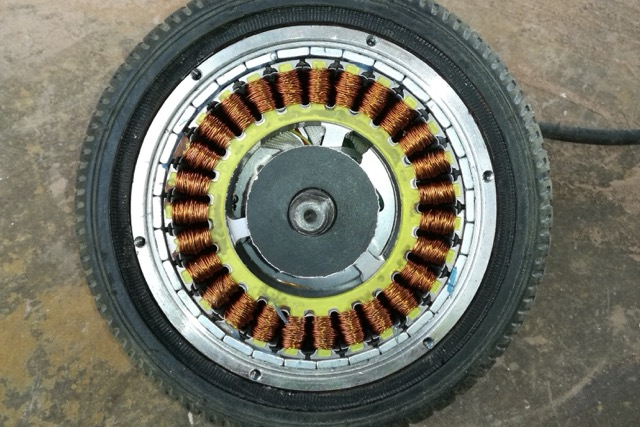
\includegraphics[width=0.5\textwidth]{fig/lec01/Wheel_hub_PMSM.jpg}
			\caption{Permanent magnet machine (source: \href{https://commons.wikimedia.org/wiki/File:Wheel_hub_motor_of_an_electric_kick_scooter,_sidepanel_removed_(2022).jpg}{Wikimedia Commons}, Andrez, \href{https://creativecommons.org/licenses/by-sa/4.0/deed.en}{CC BY-SA 4.0})}
		\end{subfigure}
		\hfill
		\begin{subfigure}[b]{0.49\textwidth}
			\centering
			\includegraphics[width=0.5\textwidth]{fig/lec01/Linear_motor.jpg}
			\caption{Linear permanent magnet machine (source: \href{https://commons.wikimedia.org/wiki/File:Linear_motor_by_Zureks.jpg}{Wikimedia Commons}, Zureks, \href{https://creativecommons.org/licenses/by-sa/4.0/n}{CC BY-SA 4.0})}
		\end{subfigure}
		\caption*{Some exemplary electrical machines} 
        \label{fig:examples_machine_drives_00}
	\end{figure}
\end{frame}


%%%%%%%%%%%%%%%%%%%%%%%%%%%%%%%%%%%%%%%%%%%%%%%%%%%%%%%%%%%%%
%% The machine as an electrical-mechanical converter %%
%%%%%%%%%%%%%%%%%%%%%%%%%%%%%%%%%%%%%%%%%%%%%%%%%%%%%%%%%%%%%
\begin{frame}
	\frametitle{The machine as an electrical-mechanical converter}
	\begin{figure}
		\centering
		\begin{subfigure}[b]{0.49\textwidth}
			\centering
			\includegraphics[width=0.9\textwidth]{fig/lec01/Block_diagram_rotational_converter.pdf}
			\caption{Rotational converter}
		\end{subfigure}
		\hfill
		\begin{subfigure}[b]{0.49\textwidth}
			\centering
			\includegraphics[width=0.9\textwidth]{fig/lec01/Block_diagram_translational_converter.pdf}
			\caption{Translational converter}
		\end{subfigure}
		\caption{Electrically and mechanically free body diagrams of motors as energy converters  with variable notation: time $t$, voltage $u$, current $i$, force $F$, displacement $x$, torque $T$ and rational speed $\omega$ (adapted from J.~B\"ocker, \textit{Elektrische Antriebstechnik}, Paderborn University, 2020)} 
        \label{fig:free_body_diagrams_motor}
	\end{figure}
\end{frame}

%%%%%%%%%%%%%%%%%%%%%%%%%%%%%%%%%%%%%%%%%%%%%%%%%%%%%%%%%%%%%
%% Some basic mechanical terms (recap) %%
%%%%%%%%%%%%%%%%%%%%%%%%%%%%%%%%%%%%%%%%%%%%%%%%%%%%%%%%%%%%%
\begin{frame}
	\frametitle{Some basic mechanical terms (recap)}
	\vspace{-0.15cm}
	\begin{table}
		\centering
		\begin{tabular}{lll}
			& Translational converter & Rotational converter \\
			\toprule
			Kinematic quantities & & \\
			Displacement / angle & $x$ & $\varepsilon$ \\
			Velocity & $v=\dot{x}$ & $\omega=\dot{\varepsilon}$ \\
			Acceleration & $a=\dot{v}=\ddot{x}$ & $\alpha=\dot{\omega}=\ddot{\varepsilon}$ \\
			Jerk & $j=\dot{a}=\ddot{v}=\dddot{x}$ & $\rho=\dot{\alpha}=\ddot{\omega}=\dddot{\varepsilon}$ \onslide<2-> \\
			\midrule
			Dynamical quantities & & \\
			Force / torque & $F$ & $T$ \\
			Mass / inertia & $m$ & $J$ \onslide<3-> \\
			\midrule
			Mechanical power & $P_\mathrm{me}=F v$ & $P_\mathrm{me}=T \omega$ \onslide<4-> \\
			Work & $W[t_0,t]=\int_{t_0}^t P_\mathrm{me}(\tau)\,\mathrm{d}\tau$ & $W[t_0,t]=\int_{t_0}^t P_\mathrm{me}(\tau)\,\mathrm{d}\tau$ \onslide<5-> \\
			Momentum / rotational momentum & $p = m v$ & $L = \omega J$ \onslide<6-> \\
			Kinetic energy & $E_\mathrm{kin} = \frac{1}{2} m v^2$ & $E_\mathrm{kin} = \frac{1}{2} J \omega^2$\\
			\bottomrule
		\end{tabular}
		\caption{Basic mechanical terms for translational and rotational converters}
		\label{tab:basic_mechanical_terms}
	\end{table}
\end{frame}

%%%%%%%%%%%%%%%%%%%%%%%%%%%%%%%%%%%%%%%%%%%%%%%%%%%%%%%%%%%%%
%% Work vs. energy (recap) %%
%%%%%%%%%%%%%%%%%%%%%%%%%%%%%%%%%%%%%%%%%%%%%%%%%%%%%%%%%%%%%
\begin{frame}
	\frametitle{Work vs. energy (recap)}
	\begin{columns}
		\begin{column}{0.5\textwidth}
			\begin{varblock}{Work}
				Work is the integral of the power over a time integral (or force over distance) and is a measure of the energy transfer.
			\end{varblock}
		\end{column}
		\begin{column}{0.5\textwidth}
			\begin{varblock}{Energy}
				Energy is the capacity to do work, that is, a quantity depending on the state of a system at a given point of time.				
			\end{varblock}
		\end{column}
		\end{columns}
		\vspace{0.5cm}
		\begin{figure}
			\centering
			\includegraphics[width=0.6\textwidth]{fig/lec01/Work_Energy.pdf}
			\caption{Illustration addressing the work vs. energy terminology (simplified Sankey diagram)}
			\label{fig:work_vs_energy}
		\end{figure}
\end{frame}

%%%%%%%%%%%%%%%%%%%%%%%%%%%%%%%%%%%%%%%%%%%%%%%%%%%%%%%%%%%%%
%% Power balance of an electrical machine %%
%%%%%%%%%%%%%%%%%%%%%%%%%%%%%%%%%%%%%%%%%%%%%%%%%%%%%%%%%%%%%
\begin{frame}
	\frametitle{Power balance of an electrical machine}
	\begin{figure}
		\centering
		\includegraphics[width=0.45\textwidth]{fig/lec01/Power_balance_machine.pdf}
		\caption{Power balance of an electrical machine (illustrated in motoric operation)}
		\label{fig:power_balance_machine}
	\end{figure}
	The power balance
	\begin{equation}
		P_\mathrm{el}(t) = P_\mathrm{me}(t) + P_\mathrm{l}(t) + \frac{\mathrm{d}}{\mathrm{d}t}E_\mathrm{i}(t)
	\end{equation}
	must hold for any point in time as energy is conserved, that is, not created or destroyed.
\end{frame}

%%%%%%%%%%%%%%%%%%%%%%%%%%%%%%%%%%%%%%%%%%%%%%%%%%%%%%%%%%%%%
%% Four quadrants of machine operation %%
%%%%%%%%%%%%%%%%%%%%%%%%%%%%%%%%%%%%%%%%%%%%%%%%%%%%%%%%%%%%%
\begin{frame}
	\frametitle{Four quadrants of machine operation}
	\begin{columns}
		\begin{column}{0.5\textwidth}
			For the steady state ($\dot{E}_{\mathrm{i}}(t)=0$), we define the \hl{machine efficiency} as the ratio of the converted energy to the input energy:
			\begin{align}
				\eta_\mathrm{mot} &= \frac{P_{\mathrm{me}}}{P_{\mathrm{el}}} = 1- \frac{P_{\mathrm{l}}}{P_{\mathrm{el}}},  \\[0.5em] 
				\onslide<2->{\eta_\mathrm{gen} &= \frac{P_{\mathrm{el}}}{P_{\mathrm{me}}} = 1- \frac{P_{\mathrm{l}}}{P_{\mathrm{me}}}.}
			\end{align}
			\onslide<3->{Hence, we need to consider in which \hl{quadrant} the machine operates as this will influence the power flow direction.}
		\end{column}
		\begin{column}{0.5\textwidth}
			\onslide<3->\begin{figure}
				\centering
				\includegraphics[width=0.75\textwidth]{fig/lec01/Machine_quadrants.pdf}
				\caption{Machine quadrants (derived from \href{https://de.wikipedia.org/wiki/Datei:Vierquadranten.svg}{Wikimedia Commons}, K. Pitter, \href{https://creativecommons.org/licenses/by-sa/3.0/deed.de}{CC BY-SA 3.0})}
				\label{fig:machine_quadrants}
			\end{figure}
		\end{column}
		\end{columns}
\end{frame}


%%%%%%%%%%%%%%%%%%%%%%%%%%%%%%%%%%%%%%%%%%%%%%%%%%%%%%%%%%%%%
%% What is an electrical drive ? %%
%%%%%%%%%%%%%%%%%%%%%%%%%%%%%%%%%%%%%%%%%%%%%%%%%%%%%%%%%%%%%
\begin{frame}
	\frametitle{What is an electrical drive ?}
	\begin{columns}
		\begin{column}{0.4\textwidth}
			\begin{varblock}{Electrical drive}
			   An electrical drive is a system that controls the torque, speed or position of an electrical machine connected to some mechanical process.
			\end{varblock}
			\vspace{0.25cm}
			\begin{itemize}
				\item<2-> Integrates the 'stupid' electrical machine into an 'intelligent' controlled system.
				\item<3-> The energy source and mechanical process ('load') are not part of the drive system.
			\end{itemize}
		\end{column}
		\begin{column}{0.6\textwidth}
			\begin{figure}
				\centering
				\includegraphics[width=0.95\textwidth]{fig/lec01/Electrical_Drive_Block_Overview.pdf}
				\caption{Block diagram of an electrical drive (adapted from J.~B\"ocker, \textit{Elektrische Antriebstechnik}, Paderborn University, 2020)}
			\end{figure}
		\end{column}
	\end{columns}
\end{frame}

%%%%%%%%%%%%%%%%%%%%%%%%%%%%%%%%%%%%%%%%%%%%%%%%%%%%%%%%%%%%%
%% Examples of electrical machine and drive applications (1) %%
%%%%%%%%%%%%%%%%%%%%%%%%%%%%%%%%%%%%%%%%%%%%%%%%%%%%%%%%%%%%%
\begin{frame}
	\frametitle{Examples of electrical machine and drive applications (1)}
	\begin{figure}
		\centering
		\begin{subfigure}[b]{0.49\textwidth}
			\centering
			\includegraphics[width=0.5\textwidth]{fig/lec01/Electric_Car_recharging.jpg}
			\caption{Electric cars (source: \href{https://commons.wikimedia.org/wiki/File:Electric_Car_recharging.jpg}{Wikimedia Commons}, M.~Movchin and F. Mueller, \href{https://creativecommons.org/licenses/by-sa/3.0/deed.en}{CC BY-SA 3.0})}
		\end{subfigure}
		\hfill
		\begin{subfigure}[b]{0.49\textwidth}
			\centering
			\includegraphics[width=0.5\textwidth]{fig/lec01/sky-farm-windmill.jpg}
			\caption{Wind turbine generators (source: \href{https://pxhere.com/en/photo/954757}{pxhere.com}, public domain)}
		\end{subfigure}
		\\
		\begin{subfigure}[b]{0.49\textwidth}
			\centering
			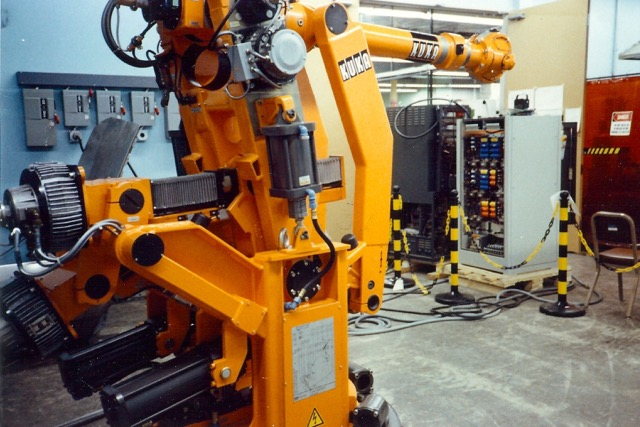
\includegraphics[width=0.5\textwidth]{fig/lec01/Automatix_KukaRobot.jpg}
			\caption{Factory robots (source: \href{https://commons.wikimedia.org/wiki/File:Automatix_KukaRobot483.agr.jpg}{Wikimedia Commons}, A.~Reinhold, \href{https://creativecommons.org/licenses/by-sa/4.0/deed.en}{CC BY-SA 4.0})}
		\end{subfigure}
		\hfill
		\begin{subfigure}[b]{0.49\textwidth}
			\centering
			\includegraphics[width=0.5\textwidth]{fig/lec01/electric_drill.jpg}
			\caption{Electric tools (source: \href{https://www.flickr.com/photos/30478819@N08/49940384798}{flickr.com},  M.~Verch, \href{https://creativecommons.org/licenses/by/2.0/}{CC BY 2.0})}
		\end{subfigure}
		\caption*{Examples of electrical machine and drive applications} 
        \label{fig:examples_machine_drives_01}
	\end{figure}
\end{frame}

%%%%%%%%%%%%%%%%%%%%%%%%%%%%%%%%%%%%%%%%%%%%%%%%%%%%%%%%%%%%%
\subsection{Application examples}
%%%%%%%%%%%%%%%%%%%%%%%%%%%%%%%%%%%%%%%%%%%%%%%%%%%%%%%%%%%%%

%%%%%%%%%%%%%%%%%%%%%%%%%%%%%%%%%%%%%%%%%%%%%%%%%%%%%%%%%%%%%
%% Examples of electrical machine and drive applications (2) %%
%%%%%%%%%%%%%%%%%%%%%%%%%%%%%%%%%%%%%%%%%%%%%%%%%%%%%%%%%%%%%
\begin{frame}
	\frametitle{Examples of electrical machine and drive applications (2)}
	% Set up a 2x2 grid of figures
	\begin{figure}
		\ContinuedFloat
		\centering
		\begin{subfigure}[b]{0.49\textwidth}
			\centering
			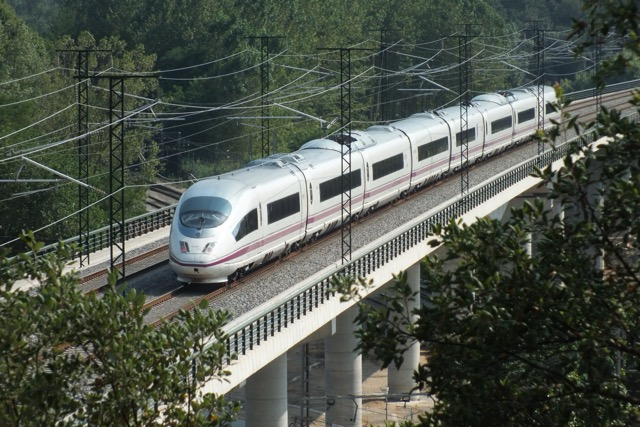
\includegraphics[width=0.5\textwidth]{fig/lec01/Train.jpg}
			\caption{High-speed trains (source: \href{https://commons.wikimedia.org/wiki/File:Fast_Train_Spain_Class_103_AVE_Siemens_Bridge_Macanet-Massanes.JPG}{Wikimedia Commons}, P.~Elektro, \href{https://creativecommons.org/licenses/by-sa/3.0/deed.en}{CC BY-SA 3.0})}
		\end{subfigure}
		\hfill
		\begin{subfigure}[b]{0.49\textwidth}
			\centering
			\includegraphics[width=0.5\textwidth]{fig/lec01/Electric_Airbus_A320.jpg}
			\caption{Electric aircraft (source: \href{https://commons.wikimedia.org/wiki/File:Electric_Airbus_A320.jpg}{Wikimedia Commons}, M.~Weinold, \href{https://creativecommons.org/licenses/by-sa/4.0/deed.en}{CC BY-SA 4.0})}
		\end{subfigure}
		\\
		\begin{subfigure}[b]{0.49\textwidth}
			\centering
			\includegraphics[width=0.5\textwidth]{fig/lec01/Pump.jpg}
			\caption{Pumps (source: \href{https://commons.wikimedia.org/wiki/File:Hammelmann_Stationary_unit_with_electric_motor.jpg}{Wikimedia Commons}, Hammelmann, \href{https://creativecommons.org/licenses/by-sa/3.0/deed.en}{CC BY-SA 3.0})}
		\end{subfigure}
		\hfill
		\begin{subfigure}[b]{0.49\textwidth}
			\centering
			\includegraphics[width=0.5\textwidth]{fig/lec01/crane.jpg}
			\caption{Cranes (source: \href{https://commons.wikimedia.org/wiki/File:Hammelmann_Stationary_unit_with_electric_motor.jpg}{Wikimedia Commons}, Belfast Dissenter, \href{https://creativecommons.org/licenses/by-sa/4.0/deed.en}{CC BY-SA 4.0})}
		\end{subfigure}
		\caption*{Examples of electrical machine and drive applications} 
        \label{fig:examples_machine_drives_02}
	\end{figure}
\end{frame}

%%%%%%%%%%%%%%%%%%%%%%%%%%%%%%%%%%%%%%%%%%%%%%%%%%%%%%%%%%%%%
%% Examples of electrical machine and drive applications (2) %%
%%%%%%%%%%%%%%%%%%%%%%%%%%%%%%%%%%%%%%%%%%%%%%%%%%%%%%%%%%%%%
\begin{frame}
	\frametitle{A broad range of nominal power ratings}
	\vspace{-0.1cm}
	\begin{figure}
		\centering
		\includegraphics[height=0.7\textheight]{fig/lec01/Power_Classes_Examples.pdf}
		\caption{Power range overview (inspired  from A.~Binder, \textit{Elektrische Maschinen und Antriebe (lecture slides)}, Darmstadt University, 2022 with additional figure sources: \href{https://www.flickr.com/photos/arthurwolf/5393520058/}{A. Wolf}, \href{https://commons.wikimedia.org/wiki/File:Wald_am_Arlberg-OeBB_Spullersee_power_plant-M1-Rotor-11ASD.jpg}{Asurnipal}, \href{https://www.flickr.com/photos/mouser-nerdbot/7042785635}{M. Williams}, \href{https://de.m.wikipedia.org/wiki/Datei:Stick_blender_Electrolux_AEG_HB_9807_-_stator_of_the_electric_motor-4313.jpg}{R. Spekking}, \href{https://commons.wikimedia.org/wiki/File:Electric_motor_and_transmission_in_a_truck.jpg}{Foxcorner}, \href{https://commons.wikimedia.org/wiki/File:E-bike_electric_motor_shimano_ep_8.jpg}{A.~Tredz} and \href{https://commons.wikimedia.org/wiki/File:2023_Corsair_SP120_RGB_Elite.jpg}{J. Halicki} under varying CC licenses) }
		\label{Power_Classes_Examples}
	\end{figure}
\end{frame}

%%%%%%%%%%%%%%%%%%%%%%%%%%%%%%%%%%%%%%%%%%%%%%%%%%%%%%%%%%%%%
%% Why are electric machines and drives important ? %%
%%%%%%%%%%%%%%%%%%%%%%%%%%%%%%%%%%%%%%%%%%%%%%%%%%%%%%%%%%%%%
\begin{frame}
	\frametitle{Why is knowledge about electric machines and drives important?}
	\begin{varblock}{Electric machines and drives are an essential pillar of the modern society}
		Without electric machines and drives, our todays society would not be possible. Starting from providing electricity via electrical generators to powering electric vehicles, tools and entire factory production lines, electric machines and drives are everywhere, that is, they enable our today's living standard. 
	\end{varblock}
	\begin{varblock}{Energy efficiency and sustainability is key}<2->
		Electric machines and drives utilize  approx. 50\,\% of the global electricity with about 8 billion electric motors in use in the EU (source: \href{https://commission.europa.eu/energy-climate-change-environment/standards-tools-and-labels/products-labelling-rules-and-requirements/energy-label-and-ecodesign/energy-efficient-products/electric-motors-and-variable-speed-drives_en}{European Commission} and \href{https://iea.blob.core.windows.net/assets/d69b2a76-feb9-4a74-a921-2490a8fefcdf/EE_for_ElectricSystems.pdf}{International Energy Agency}). Therefore, improving their efficiency is an essential factor to reduce the global energy consumption and the associated CO$_2$ emissions.
	\end{varblock}
\end{frame}

%%%%%%%%%%%%%%%%%%%%%%%%%%%%%%%%%%%%%%%%%%%%%%%%%%%%%%%%%%%%%
\subsection{Course organization}
%%%%%%%%%%%%%%%%%%%%%%%%%%%%%%%%%%%%%%%%%%%%%%%%%%%%%%%%%%%%%

%%%%%%%%%%%%%%%%%%%%%%%%%%%%%%%%%%%%%%%%%%%%%%%%%%%%%%%%%%%%%
%% Learning objectives %%
%%%%%%%%%%%%%%%%%%%%%%%%%%%%%%%%%%%%%%%%%%%%%%%%%%%%%%%%%%%%%
\begin{frame}
	\frametitle{Learning objectives}
	\begin{itemize}
		\item Understand the generation of magnetic fields, force formation and voltage induction in electrical machines.
		\item<2-> Differentiate the main types of electrical machines and drives:
		\begin{itemize}
			\item DC machines. 
			\item Induction machines.
			\item Synchronous machines.
			\item And their plentiful variants \ldots
		\end{itemize}
		\item<3-> Understand their basic design and operation principles.
		\item<4-> Analyze the operation of electrical machines and drives:
		\begin{itemize}
			\item in steady state and
			\item in transient conditions.
		\end{itemize} 
		\item<5-> Have fun learning about electrical machines and drives.
	\end{itemize}
\end{frame}


%%%%%%%%%%%%%%%%%%%%%%%%%%%%%%%%%%%%%%%%%%%%%%%%%%%%%%%%%%%%%
%% Necessary prior knowledge %%
%%%%%%%%%%%%%%%%%%%%%%%%%%%%%%%%%%%%%%%%%%%%%%%%%%%%%%%%%%%%%
\begin{frame}
	\frametitle{Necessary prior knowledge for this course}
	You should have a basic understanding of the following topics:
	\begin{itemize}
		\item Analysis basics (e.g., complex analysis and differential equations)
		\item Linear algebra basics (e.g., vector and matrix operations)
		\item Basic knowledge of electrical circuit theory and components
	\end{itemize}
	\vspace{0.5cm}
	\onslide<2->What we will \underline{not} cover, that is, you do not need to know (covered in separate courses):
	\begin{itemize}
		\item Control engineering (design drive controllers)
		\item Power electronics (design switchable actuators)
	\end{itemize}
\end{frame}

%%%%%%%%%%%%%%%%%%%%%%%%%%%%%%%%%%%%%%%%%%%%%%%%%%%%%%%%%%%%%
%% Recommended reading %%
%%%%%%%%%%%%%%%%%%%%%%%%%%%%%%%%%%%%%%%%%%%%%%%%%%%%%%%%%%%%%
\begin{frame}
	\frametitle{Recommended reading}
	\begin{itemize}
		\item A. Binder, Elektrische Maschinen und Antriebe (in German), Vol. 2, Springer, 2017
		\item D. Schr\"oder and R. Kennel, Elektrische Antriebe: Grundlagen (in German), Vol. 7, Springer Vieweg, 2021
		\item A. Huges and B. Drury, Electric Motors and Drives: Fundamentals, Types and Applications, Vol. 5, Newnes, 2019
		\item S. Chapman, Electric Machinery Fundamentals, Vol. 5, McGraw-Hill, 2011
		\item I. Boldea and S. Nasar, Electric Drives, Vol. 3, CRC Press, 2022
	\end{itemize}
\end{frame} % Overview / introduction
\section{Fundamental electromagnetic principles and magnetic materials}

%%%%%%%%%%%%%%%%%%%%%%%%%%%%%%%%%%%%%%%%%%%%%%%%%%%%%%%%%%%%%
\subsection{Amp\`ere's--Maxwell equation}
%%%%%%%%%%%%%%%%%%%%%%%%%%%%%%%%%%%%%%%%%%%%%%%%%%%%%%%%%%%%%
%%%%%%%%%%%%%%%%%%%%%%%%%%%%%%%%%%%%%%%%%%%%%%%%%%%%%%%%%%%%%

%% Ampere's circuital law: magnetic field strength %%
%%%%%%%%%%%%%%%%%%%%%%%%%%%%%%%%%%%%%%%%%%%%%%%%%%%%%%%%%%%%%
\begin{frame}
	\frametitle{Amp\`ere's circuital law: magnetic field strength}
	\begin{columns}
		\begin{column}{0.55\textwidth}
			Relates the circulation of a \hl{magnetic field} $\bm{H}$ around a closed loop to the electric current passing through the loop:
            \begin{align}
                \mbox{Integral form:} \quad &\oint_{\partial S} \bm{H} \cdot \mathrm{d}\bm{s} = I_{\mathrm{f}},\\
                \mbox{Differential form:} \quad &\nabla \times \bm{H} = \bm{J}_{\mathrm{f}}. 
                \label{eq:ampere_law}
            \end{align}
            Here, $\bm{J}_{\mathrm{f}}$ is the \hl{free current density}, and $I_{\mathrm{f}}$ is the \hl{free current} enclosed by the loop $\partial S$. 
            \vspace{0.25cm}
            \begin{itemize}
                \item<2-> Free current: current that is not bound to a material (i.e., without polarization and magnetization currents).
                \item<3-> SI-units: $[H] = \si{\ampere\per\metre}$, $[J] = \si{\ampere\per\metre\squared}$
            \end{itemize}
		\end{column}
        \hfill
		\begin{column}{0.4\textwidth}
			\begin{figure}
				\centering
				\includegraphics[height=0.7\textheight]{fig/lec02/Magnetic_field_strength_simple_conductor.pdf}
				\caption{Illustration of the magnetic field strength $\bm{H}$ around a simple conductor}
			\end{figure}
		\end{column}
		\end{columns}
\end{frame}

%%%%%%%%%%%%%%%%%%%%%%%%%%%%%%%%%%%%%%%%%%%%%%%%%%%%%%%%%%%%%
%% Ampere's circuital law: free current example %%
%%%%%%%%%%%%%%%%%%%%%%%%%%%%%%%%%%%%%%%%%%%%%%%%%%%%%%%%%%%%%
\begin{frame}
	\frametitle{Amp\`ere's circuital law: free current example}
	\begin{columns}
		\begin{column}{0.55\textwidth}
			What is the free current $I_{\mathrm{f}}$ enclosed by the loop $\partial S$?
            \begin{itemize}
                \item<2-> The current $I_1$ flows in the direction of the loop $\partial S$ (according to right-hand rule).
                \item<3-> The current $I_1$ must be counted $N$ times due to the $N$ turns of wire around the loop $\partial S$.
                \item<4-> The current $I_2$ flows in the opposite direction of the loop $\partial S$ (according to right-hand rule).
                \item<5-> Result:
            \end{itemize}
            \vspace{0.25cm}
            \onslide<5->{\begin{equation*}
                I_\mathrm{f} = N \cdot I_1 - I_2.
            \end{equation*}}
		\end{column}
        \hfill
		\begin{column}{0.45\textwidth}
			\begin{figure}
				\centering
				\includegraphics[height=0.5\textheight]{fig/lec02/Magnetic_field_strength_multiple_conductors.pdf}
				\caption{Arrangement with two electrical conductors}
			\end{figure}
		\end{column}
		\end{columns}
\end{frame}

%%%%%%%%%%%%%%%%%%%%%%%%%%%%%%%%%%%%%%%%%%%%%%%%%%%%%%%%%%%%%
%% Ampere's circuital law: simple solenoid  example%%
%%%%%%%%%%%%%%%%%%%%%%%%%%%%%%%%%%%%%%%%%%%%%%%%%%%%%%%%%%%%%
\begin{frame}
	\frametitle{Amp\`ere's circuital law: simple solenoid example}
	\begin{columns}
		\begin{column}{0.575\textwidth}
			Ampere's law for \hl{magnetic flux density} $\bm{B}$ in vacuum:
            \begin{align}
                \mbox{Integral form:} \quad &\oint_{\partial S} \bm{B} \cdot \mathrm{d}\bm{s} = \mu_0 I,\\
                \mbox{Differential form:} \quad &\nabla \times \bm{B} = \mu_0\bm{J}. 
            \end{align}
            Here, $\mu_0$ is the \hl{permeability} of free space, $\bm{J}$ is the total current density and $I$ is the total current enclosed by the loop $\partial S$. 
            \vspace{0.25cm}
            \begin{itemize}
                \item<2-> SI-unit: $[B] = \si{\tesla} = \si{\volt\second\per\metre\squared} = \si{\newton\per\ampere\per\metre}$
                \item<3-> Example contour $\partial S$  on the right covering $N$ turns and length $l$ (flux density within solenoid):
            \end{itemize}
            \onslide<4->{$$\oint_{\partial S} \bm{B} \cdot \mathrm{d}\bm{s} = N \mu_0 I  \Leftrightarrow B = \frac{N \mu_0 I}{l}$$}
		\end{column}
        \hfill
		\begin{column}{0.425\textwidth}
            \vspace{-0.2cm}
			\begin{figure}
				\centering
				\includegraphics[height=0.68\textheight]{fig/lec02/Solenoid_Ampere_law.pdf}
				\caption{Magnetic flux density evaluated at the contour $\partial \bm{S}$  (adapted from: \href{https://commons.wikimedia.org/wiki/File:Solenoid_and_Ampere_Law.png}{Wikimedia Commons}, Goodphy, \href{https://creativecommons.org/licenses/by-sa/4.0/deed.en}{CC BY-SA 4.0})}
			\end{figure}
		\end{column}
		\end{columns}
\end{frame}

%%%%%%%%%%%%%%%%%%%%%%%%%%%%%%%%%%%%%%%%%%%%%%%%%%%%%%%%%%%%%
%% Shortcomings of the Ampere's circuital law %%
%%%%%%%%%%%%%%%%%%%%%%%%%%%%%%%%%%%%%%%%%%%%%%%%%%%%%%%%%%%%%
\begin{frame}
	\frametitle{Shortcomings of the Amp\`ere's circuital law}
	\begin{columns}
		\begin{column}{0.55\textwidth}
			Applying Amp\`ere's circuital law to a capacitor with a changing \hl{electric field} $\bm{E}$ leads to a contradiction:
            \begin{itemize}
                \item Applying \eqref{eq:ampere_law} to $S_1$ yields:
                $$\oint_{\partial S_1} \bm{H} \cdot \mathrm{d}\bm{s} = I.$$
                \item<2-> In the case of $S_2$ we receive:
                $$\oint_{\partial S_2} \bm{H} \cdot \mathrm{d}\bm{s} = 0.$$
                \item<3-> However, both surfaces share the same bounding contour $\partial S$.
                \item<4-> Issue: The magnetic field strength $\bm{H}$ is not able to describe the displacement current.
            \end{itemize}
		\end{column}
        \hfill
		\begin{column}{0.45\textwidth}
			\begin{figure}
				\centering
				\includegraphics[height=0.55\textheight]{fig/lec02/Displacement_current_in_capacitor.pdf}
				\caption{Surfaces $S_1$ and $S_2$ share the same bounding contour $\partial S$. However, $S_1$ is pierced by conduction current, while $S_2$ is pierced by displacement current (adapted from: \href{https://commons.wikimedia.org/wiki/File:Displacement_current_in_capacitor.svg}{Wikimedia Commons}, public domain).}
			\end{figure}
		\end{column}
		\end{columns}
\end{frame}

%%%%%%%%%%%%%%%%%%%%%%%%%%%%%%%%%%%%%%%%%%%%%%%%%%%%%%%%%%%%%
%% The Ampere--Maxwell equation %%
%%%%%%%%%%%%%%%%%%%%%%%%%%%%%%%%%%%%%%%%%%%%%%%%%%%%%%%%%%%%%
\begin{frame}
	\frametitle{The Amp\`ere -- Maxwell equation}
	\begin{columns}
		\begin{column}{0.6\textwidth}
			The \hl{charge} $Q$ of capacitor is:
            $$Q = \oint_{S_2} \bm{D}\cdot \mathrm{d}\bm{S}.$$
            \onslide<2->{If the \hl{electric flux density} $\bm{D} = \varepsilon_0\varepsilon_\mathrm{r} \bm{E}$ changes, a displacement current results:
            $$I_{\mathrm{d}} = \frac{\mathrm{d}}{\mathrm{d} t} \oint_{S_2} \bm{D}\cdot \mathrm{d}\bm{S}$$}
            \begin{itemize}
                \item<3-> Is not a classical electric current (moving charges) but a term to describe the changing electric field.
                \item<4-> Above, $\varepsilon_0$ is the \hl{vacuum permittivity} and $\varepsilon_\mathrm{r}$ is the \hl{relative permittivity} of a material.
            \end{itemize}
		\end{column}
        \hfill
		\begin{column}{0.4\textwidth}
			\begin{figure}
				\centering
				\includegraphics[height=0.65\textheight]{fig/lec02/Maxwell_integral_displacement_current.pdf}
				\caption{Illustration for calculating the displacement current (adapted from: \href{https://commons.wikimedia.org/wiki/File:Maxwell_integral_displacement_current.svg}{Wikimedia Commons}, public domain).}
			\end{figure}
		\end{column}
		\end{columns}
\end{frame}

%%%%%%%%%%%%%%%%%%%%%%%%%%%%%%%%%%%%%%%%%%%%%%%%%%%%%%%%%%%%%
%% The Ampere--Maxwell equation (cont.)%%
%%%%%%%%%%%%%%%%%%%%%%%%%%%%%%%%%%%%%%%%%%%%%%%%%%%%%%%%%%%%%
\begin{frame}
	\frametitle{The Amp\`ere -- Maxwell equation (cont.)}
        Adding the displacement current to \eqref{eq:ampere_law} we receive the Amp\`ere -- Maxwell equation:
            \begin{align}    
            \mbox{Integral form:} \quad  &\int_{\partial S} \bm{H} \cdot \mathrm{d}\bm{s} = \iint_{S}\left(\bm{J}_\mathrm{f} + \frac{\mathrm{d}}{\mathrm{d} t} \bm{D} \right)\cdot\mathrm{d}\bm{S}, \\
            \mbox{Differential form:} \quad &\nabla \times \bm{H} = \bm{J}_\mathrm{f} +  \frac{\partial\bm{D}}{\partial t}. 
            \label{eq:ampere_maxwell_law}
        \end{align}
        \vspace{0.5cm}
        \begin{itemize}
            \item SI-unit: $[D] = \si{\coulomb\per\metre\squared}$
            \item SI-unit: $[E] = \si{\volt\per\metre}$
            \item $\varepsilon_0 \approx \SI{8.854e-12}{\farad\per\metre}$
        \end{itemize}
\end{frame}

%%%%%%%%%%%%%%%%%%%%%%%%%%%%%%%%%%%%%%%%%%%%%%%%%%%%%%%%%%%%%
\subsection{Magnetic flux, flux linkage and inductance}
%%%%%%%%%%%%%%%%%%%%%%%%%%%%%%%%%%%%%%%%%%%%%%%%%%%%%%%%%%%%%

%%%%%%%%%%%%%%%%%%%%%%%%%%%%%%%%%%%%%%%%%%%%%%%%%%%%%%%%%%%%%
%% Magnetic flux and flux linkage %%
%%%%%%%%%%%%%%%%%%%%%%%%%%%%%%%%%%%%%%%%%%%%%%%%%%%%%%%%%%%%%
\begin{frame}
	\frametitle{Magnetic flux and flux linkage}
	\begin{columns}
		\begin{column}{0.575\textwidth}
			The \hl{magnetic flux} $\phi$ is the surface integral of the normal component of $\bm{B}$ over that surface:
            \begin{align}
                \phi = \iint_{S} \bm{B} \cdot \mathrm{d}\bm{S}. 
            \end{align}
            \onslide<2->{As there are no magnetic monopoles, the magnetic flux through a closed surface (which is covering a volume without holes) is always zero:
            \begin{align}
                \oint_{S} \bm{B} \cdot \mathrm{d}\bm{S} = 0.
            \end{align}}
            \onslide<3->{The \hl{flux linkage} $\psi$ is the product of the magnetic flux $\phi$ and the number of turns $N$ of a coil:
            \begin{align}
                \psi = N  \phi.
            \end{align}}
		\end{column}
        \hfill
		\begin{column}{0.425\textwidth}
            \vspace{-0.4cm}
			\begin{figure}
				\centering
				\includegraphics[height=0.68\textheight]{fig/lec02/Solenoid_Flux.pdf}
				\caption{Magnetic flux $\phi$ evaluated at the surface $\bm{S}$  (adapted from: \href{https://commons.wikimedia.org/wiki/File:Solenoid_and_Ampere_Law.png}{Wikimedia Commons}, Goodphy, \href{https://creativecommons.org/licenses/by-sa/4.0/deed.en}{CC BY-SA 4.0})}
                \label{fig:Solenoid_Flux}
			\end{figure}
		\end{column}
		\end{columns}
\end{frame}




%%%%%%%%%%%%%%%%%%%%%%%%%%%%%%%%%%%%%%%%%%%%%%%%%%%%%%%%%%%%%
%% Magnetic leakage flux %%
%%%%%%%%%%%%%%%%%%%%%%%%%%%%%%%%%%%%%%%%%%%%%%%%%%%%%%%%%%%%%
\begin{frame}
	\frametitle{Magnetic leakage flux}
	\begin{columns}
		\begin{column}{0.48\textwidth}
			\begin{itemize}
                \item<2-> In the scenarios with multiple coils, the magnetic flux generated by one coil will influence also the other coils.
                \item<2-> Exception: two coils are perfectly perpendicular to each other.
                \item<2-> However, the magnetic flux typically does not fully couple with the other coils
                \item<2-> The difference is the \hl{leakage flux} $\phi_\sigma$.
            \end{itemize}
		\end{column}
        \hfill
		\begin{column}{0.48\textwidth}
            \vspace{-0.2cm}
			\begin{figure}
				\centering
				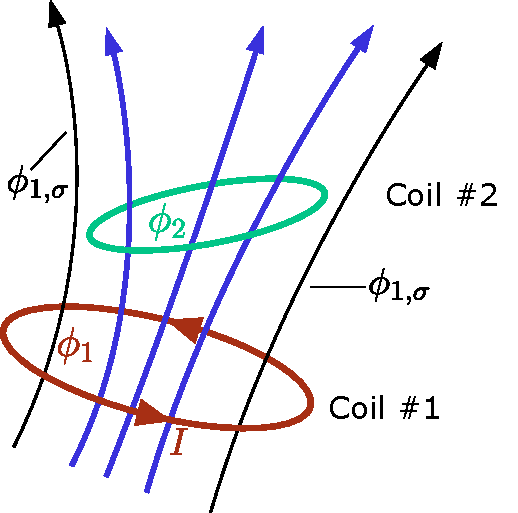
\includegraphics[height=0.55\textheight]{fig/lec02/Leakage_flux.pdf}
				\caption{The magnetic flux $\phi_1$ generated by the current $I$ does only partly couple with the second coil, while the difference $\phi_1-\phi_2$ is the leakage flux (adapted from: \href{https://commons.wikimedia.org/wiki/File:Mutual_Inductivity.svg}{Wikimedia Commons}, M. Wacenovsky, public domain)}
			\end{figure}
		\end{column}
		\end{columns}
\end{frame}

%%%%%%%%%%%%%%%%%%%%%%%%%%%%%%%%%%%%%%%%%%%%%%%%%%%%%%%%%%%%%
%% Inductance %%
%%%%%%%%%%%%%%%%%%%%%%%%%%%%%%%%%%%%%%%%%%%%%%%%%%%%%%%%%%%%%
\begin{frame}
	\frametitle{Inductance}
	The \hl{inductance} $L$ describes the ratio between the magnetic flux linkage $\psi(t)$ to the current $i(t)$:
    \begin{align}
        \psi(t) = L i(t).
    \end{align}
    \pause
    \textbf{Example}:  From the solenoid in \figref{fig:Solenoid_Flux} we know that the magnetic flux linkage $\psi$ is:
    $$\psi = N \iint_{S} \bm{B} \cdot \mathrm{d}\bm{S}= \frac{1}{l}N^2 \mu_0 I \pi r^2 $$
    with $r$ being the radius of the solenoid. \pause Hence, the inductance $L$ is:
    $$L = \frac{\psi}{I} = \frac{N^2 \mu_0 \pi r^2}{l}.$$
    \begin{itemize}
        \item SI-unit: $[L] = \si{\henry} = \si{\volt\second\per\ampere}$
        \item The inductance is an important parameter describing inductive systems.
    \end{itemize}
\end{frame}

%%%%%%%%%%%%%%%%%%%%%%%%%%%%%%%%%%%%%%%%%%%%%%%%%%%%%%%%%%%%%
%% Self and mutual inductance %%
%%%%%%%%%%%%%%%%%%%%%%%%%%%%%%%%%%%%%%%%%%%%%%%%%%%%%%%%%%%%%
\begin{frame}
	\frametitle{Self and mutual inductance}
    \begin{columns}
		\begin{column}{0.45\textwidth}
            Based on the inductive coupling between the two coils from \figref{fig:Transformer3d_col3}, we can define the magnetic flux matrix:
            \begin{equation}
                \bm{\phi} = \begin{bmatrix} \phi_{11} & \phi_{12} \\ \phi_{21} & \phi_{22} \end{bmatrix} .
                \label{eq:flux_matrix_transformer}
            \end{equation}
            \vspace{-0.2cm}
			\begin{itemize}
                \item<2-> $\phi_{11}$: magnetic flux component of coil 1 due to its own current $i_1$
                \item<3-> $\phi_{12}$: magnetic flux component of coil 1 due to the current $i_2$ in coil 2
                \item<4-> $\phi_{21}$: magnetic flux component of coil 2 due to the current $i_1$ in coil 1
                \item<5-> $\phi_{22}$: magnetic flux component of coil 2 due to its own current $i_2$
            \end{itemize}
		\end{column}
        \hfill
		\begin{column}{0.525\textwidth}
			\begin{figure}
				\centering
				\includegraphics[height=0.575\textheight]{fig/lec02/Transformer3d_col3.pdf}
				\caption{Two coils coupled via a common core (adapted from: \href{https://commons.wikimedia.org/wiki/File:Transformer3d_col3.svg}{Wikimedia Commons}, Bill C., \href{https://creativecommons.org/licenses/by-sa/3.0/deed.en}{CC~BY-SA~3.0})}
                \label{fig:Transformer3d_col3}
			\end{figure}
		\end{column}
		\end{columns}
\end{frame}

%%%%%%%%%%%%%%%%%%%%%%%%%%%%%%%%%%%%%%%%%%%%%%%%%%%%%%%%%%%%%
%% Self and mutual inductance (cont.) %%
%%%%%%%%%%%%%%%%%%%%%%%%%%%%%%%%%%%%%%%%%%%%%%%%%%%%%%%%%%%%%
\begin{frame}
	\frametitle{Self and mutual inductance (cont.)}
    Utilizing the \hl{permeance} definition (\enquote{magnetic conductance}) 
    \begin{equation}
        \Lambda = \frac{\phi}{N i},
    \end{equation}
    \pause
    we can represent \eqref{eq:flux_matrix_transformer} as:
    \begin{equation}
        \phi_{11} = \Lambda_{11} N_1 i_1, \quad \phi_{12} = \Lambda_{12} N_2 i_2, \quad \phi_{21} = \Lambda_{21} N_1 i_1, \quad \phi_{22} = \Lambda_{22} N_2 i_2.
    \end{equation}
    \pause
    The resulting flux linkage per coil is then:
    \begin{equation}
        \begin{alignedat}{3}
        \psi_1 &= N_1\left(\phi_{11} + \phi_{21} + \phi_{12}\right), \quad && \psi_2 && =  N_2\left(\phi_{22} + \phi_{12} + \phi_{21}\right),\\ \pause
               &=\underbrace{\left(\Lambda_{11}N_1^2+\Lambda_{21}N_1^2\right)}_{L_1}i_1 + \underbrace{\Lambda_{12}N_1N_2}_{M_{12}}i_2, \quad && && =\underbrace{\left(\Lambda_{22}N_2^2+\Lambda_{12}N_1^2\right)}_{L_2}i_2 + \underbrace{\Lambda_{21}N_1N_2}_{M_{21}}i_1. 
        \end{alignedat}
        \label{eq:flux_linkage_transformer}
    \end{equation}
    Above, $L_1$ and $L_2$ are the \hl{self-inductances}, $M_{12}$ and $M_{21}$ are the \hl{mutual inductances}.
\end{frame}

%%%%%%%%%%%%%%%%%%%%%%%%%%%%%%%%%%%%%%%%%%%%%%%%%%%%%%%%%%%%%
%% Self and mutual inductance (cont.) %%
%%%%%%%%%%%%%%%%%%%%%%%%%%%%%%%%%%%%%%%%%%%%%%%%%%%%%%%%%%%%%
\begin{frame}
	\frametitle{Self and mutual inductance (cont.)}
    Hence, we can define the flux linkages of both coils using the following \hl{inductance matrix}:
    \begin{equation}
        \bm{\psi} = \begin{bmatrix} \psi_1 \\ \psi_2 \end{bmatrix} = \begin{bmatrix} L_1 & M_{12} \\ M_{21} & L_2 \end{bmatrix} \begin{bmatrix} i_1 \\ i_2 \end{bmatrix} = \bm{L}\bm{i}.
        \label{eq:flux_linkage_matrix_transformer}
    \end{equation}
    \pause
    Due to the symmetry of the inductive coupling, the mutual inductances are identical:
    \begin{equation}
        M_{12} = M_{21} = M.
    \end{equation}
    \pause
    Based on \eqref{eq:flux_linkage_transformer}, we can also split the self-inductance $L_i$ of the $i$-th coil into the sum of the \hl{leakage inductance} $L_{i,\sigma}$ and the \hl{magnetizing inductance} $L_{i,\mathrm{m}}$:
    \begin{equation}
        L_i = L_{i,\sigma} + L_{i,\mathrm{m}} = \Lambda_{ii}N_i^2 + \Lambda_{ji}N_i^2 \quad \mbox{with} \quad i \neq j. 
        \label{eq:inductance_split}
    \end{equation}
    \pause
    Finally, we can define the \hl{coupling coefficient} $k$ as:
    \begin{equation}
        k = \frac{M}{\sqrt{L_1 L_2}}, \qquad 0 \leq k \leq 1,
        \label{eq:coupling_coefficient}
    \end{equation}
    which indicates how strong or week the inductive coupling between the coils is.
\end{frame}

%%%%%%%%%%%%%%%%%%%%%%%%%%%%%%%%%%%%%%%%%%%%%%%%%%%%%%%%%%%%%
\subsection{Magnetic material properties}
%%%%%%%%%%%%%%%%%%%%%%%%%%%%%%%%%%%%%%%%%%%%%%%%%%%%%%%%%%%%%
%%%%%%%%%%%%%%%%%%%%%%%%%%%%%%%%%%%%%%%%%%%%%%%%%%%%%%%%%%%%%

%%%%%%%%%%%%%%%%%%%%%%%%%%%%%%%%%%%%%%%%%%%%%%%%%%%%%%%%%%%%%
%% Boosting the magnet field with ferromagnetic materials %%
%%%%%%%%%%%%%%%%%%%%%%%%%%%%%%%%%%%%%%%%%%%%%%%%%%%%%%%%%%%%%
\begin{frame}
	\frametitle{Boosting the magnet field with ferromagnetic materials}
	\begin{columns}
		\begin{column}{0.575\textwidth}
			While $\bm{H}$ depends on the currents applied to an object, $\bm{B}$ depends on the material properties of the object. In free space (vacuum), the relation is linear and represented by the magnetic constant $\mu_0$:
            \begin{align}
                \bm{B} = \mu_0 \bm{H} \quad \mbox{with} \quad \mu_0 \approx \SI{4 \pi e-7}{\newton\per\ampere\squared}.
            \end{align}
            \onslide<2->{To boost $\bm{B}$ for a given $\bm{H}$, ferromagnetic materials are typically used. These materials have a high \hl{relative magnetic permeability} $\mu_{\mathrm{r}}$:
            \begin{align}
                \bm{B} = \mu \bm{H} = \mu_0 \mu_{\mathrm{r}} \bm{H}.
                \label{eq:linear_permeability} 
            \end{align}}
            \onslide<3->{Note that $\mu_{\mathrm{r}}$ is a dimensionless quantity and that \eqref{eq:linear_permeability} assumes linear and isotropic material behavior.}
		\end{column}
        \hfill
		\begin{column}{0.425\textwidth}
            \vspace{-0.2cm}
			\begin{figure}
				\centering
				\includegraphics[height=0.68\textheight]{fig/lec02/Electromagnet_with_gap.pdf}
				\caption{Simplified magnetic field lines of an iron yoke with a coil  (adapted from: \href{https://en.m.wikipedia.org/wiki/File:Electromagnet_with_gap.svg}{Wikimedia Commons}, public domain)}
			\end{figure}
		\end{column}
		\end{columns}
\end{frame}

%%%%%%%%%%%%%%%%%%%%%%%%%%%%%%%%%%%%%%%%%%%%%%%%%%%%%%%%%%%%%
%% Relative permeability and magnetic saturation %%
%%%%%%%%%%%%%%%%%%%%%%%%%%%%%%%%%%%%%%%%%%%%%%%%%%%%%%%%%%%%%
\begin{frame}
	\frametitle{Relative permeability and magnetic saturation}
	\begin{columns}
		\begin{column}{0.575\textwidth}
			\begin{table}
            \centering
            \begin{tabular}{lc}
                \toprule
                Material & $\mu_{\mathrm{r}}$ (range)\\
                \midrule
                Air / copper / aluminum & $(\approx)$1 \\ 
                Iron (99.8\,\% pure) & 5000\\
                Electrical steel & 2000 - 35000\\
                Ferrite & 200 - 20000\\
                \bottomrule
            \end{tabular}
            \caption{Typical relative permeabilities of materials}
            \label{tab:rel_permeabilities}
            \end{table}
        \onslide<2->{Linear magnetic behavior ($\mu_{\mathrm{r}}=\mbox{const.}$) is only a local approximation. When considering larger $H$ ranges, the (differential) permeability becomes nonlinear:
        \begin{align}
            \mu_\mathrm{r}(H) =  \frac{\mathrm{d}B}{\mathrm{d}H}.
        \end{align}}
		\end{column}
        \hfill
		\begin{column}{0.425\textwidth}
            \onslide<2->
			\begin{figure}
				\centering
				\includegraphics[height=0.5\textheight]{fig/lec02/Permeability_of_ferromagnet.pdf}
				\caption{Illustrative magnetization curves for ferromagnets (and ferrimagnets) and corresponding permeabilities  (adapted from: \href{https://commons.wikimedia.org/wiki/File:Permeability_of_ferromagnet_by_Zureks.svg}{Wikimedia Commons}, public domain)}
                \label{fig:Permeability_of_ferromagnet}
			\end{figure}
		\end{column}
		\end{columns}
\end{frame}


%%%%%%%%%%%%%%%%%%%%%%%%%%%%%%%%%%%%%%%%%%%%%%%%%%%%%%%%%%%%%
%% Magnetic domains (1) %%
%%%%%%%%%%%%%%%%%%%%%%%%%%%%%%%%%%%%%%%%%%%%%%%%%%%%%%%%%%%%%
\begin{frame}
	\frametitle{Magnetic domains (1)}
    \begin{columns}
	\begin{column}{0.48\textwidth}
    \begin{itemize}
        \item Magnetic domains are regions within a material where the magnetic moments of atoms are aligned (\csqoutes{mini magnets}).
        \item The magnetization within each domain points in a uniform direction, but the magnetization of different domains may point in different directions.
    \end{itemize}
    \end{column}
    \hfill
    \begin{column}{0.52\textwidth}
        \onslide{\begin{figure}
            \centering
            \movie{\includegraphics[height=0.3\textheight]{fig/lec02/Moving_magnetic_domains_preview.png}}{fig/lec02/Moving_magnetic_domains.gif}
            \caption{Animation of moving domain walls (source: \href{https://commons.wikimedia.org/wiki/File:Moving_magnetic_domains_by_Zureks.gif}{Wikimedia Commons}, Zureks, \href{https://creativecommons.org/licenses/by-sa/3.0/deed.en}{CC BY-SA 3.0})}
        \end{figure}}
    \end{column}
\end{columns}
\begin{figure}
\begin{columns}
	\begin{column}{0.6\textwidth}
            \centering
            \includegraphics[width=0.9\textwidth]{fig/lec02/Growing-magnetic-domains.pdf}
    \end{column}
    \begin{column}{0.35\textwidth}
        \caption{\raggedright Change of magnetic domains due to an external magnetic field  (adapted from: \href{https://de.wikipedia.org/wiki/Datei:Growing-magnetic-domains.svg}{Wikimedia Commons}, M. Run, \href{https://creativecommons.org/licenses/by-sa/4.0/deed.en}{CC BY-SA 4.0})}
    \end{column}
\end{columns}
\end{figure}
\end{frame}

%%%%%%%%%%%%%%%%%%%%%%%%%%%%%%%%%%%%%%%%%%%%%%%%%%%%%%%%%%%%%
%% Magnetic domains (2) %%
%%%%%%%%%%%%%%%%%%%%%%%%%%%%%%%%%%%%%%%%%%%%%%%%%%%%%%%%%%%%%
\begin{frame}
	\frametitle{Magnetic domains (2)}
    \begin{itemize}
        \item A large region of material with a constant magnetization throughout creates a large magnetic field (diagram a) below). This requires a lot of magnetostatic energy stored in the field. 
        \item<2-> To reduce this energy, the sample can ``split'' into two domains, with the magnetization in opposite directions in each domain which reduces the overall field (diagram b) below).
        \item<3->  To reduce the field energy further, each of these domains can split also, resulting in smaller parallel domains with magnetization in alternating directions, with smaller amounts of field outside the material (diagram c) below).
    \end{itemize}
\begin{figure}
\begin{columns}
	\begin{column}{0.55\textwidth}
            \centering
            \includegraphics[width=0.8\textwidth]{fig/lec02/Magnetic_domains_energy_min.png}
    \end{column}
    \begin{column}{0.4\textwidth}
        \caption{\raggedright Simplified representation of the formation of magnetic domains on the basis of energy minimization  (source: \href{https://commons.wikimedia.org/wiki/File:Powstawanie_domen_by_Zureks.png}{Wikimedia Commons}, public domain)}
    \end{column}
\end{columns}
\end{figure}
\end{frame}

%%%%%%%%%%%%%%%%%%%%%%%%%%%%%%%%%%%%%%%%%%%%%%%%%%%%%%%%%%%%%
%% Hysteresis %%
%%%%%%%%%%%%%%%%%%%%%%%%%%%%%%%%%%%%%%%%%%%%%%%%%%%%%%%%%%%%%
\begin{frame}
	\frametitle{Hysteresis}
	\begin{columns}
		\begin{column}{0.575\textwidth}
            \begin{itemize}
                \item Material defects lead to small, random jumps in magnetization called Barkhausen jumps.
                \item Domain walls move irregularly.
                \item<2-> Process also depends on the history of the magnetization process (dynamic system).
            \end{itemize}
			\begin{figure}
                \centering
                \movie{\includegraphics[height=0.3\textheight]{fig/lec02/Barkhausen_jump_preview.png}}{fig/lec02/Barkhausen_jump.gif}
                \caption{Animation of the Barkhausen jump (source: \href{https://commons.wikimedia.org/wiki/File:Barkhausensprung.gif}{Wikimedia Commons},  public domain)}
            \end{figure}
		\end{column}
        \hfill
		\begin{column}{0.425\textwidth}
            \vspace{-0.2cm}
			\onslide<2->\begin{figure}
				\centering
				\includegraphics[height=0.5\textheight]{fig/lec02/Ferromagnet_magnetization_and_magnetic_domains_and_hysteresis.pdf}
				\caption{Simplified hysteresis curve in first quadrant with magnetic domains illustration (adapted from: \href{https://commons.wikimedia.org/wiki/File:Ferromagnet_magnetization_and_magnetic_domains_and_hysteresis.svg}{Wikimedia Commons}, Fralama, \href{https://creativecommons.org/licenses/by-sa/3.0/deed.enn}{CC BY-SA 3.0})}
			\end{figure}
		\end{column}
		\end{columns}
\end{frame}

%%%%%%%%%%%%%%%%%%%%%%%%%%%%%%%%%%%%%%%%%%%%%%%%%%%%%%%%%%%%%
%% Hysteresis curve and losses %%
%%%%%%%%%%%%%%%%%%%%%%%%%%%%%%%%%%%%%%%%%%%%%%%%%%%%%%%%%%%%%
\begin{frame}
	\frametitle{Hysteresis curve and losses}
	\begin{columns}
		\begin{column}{0.5\textwidth}
            \begin{itemize}
                \item With an external and varying field $H$, a closed hysteresis curve is obtained.
                \item<2-> Traversing through the curve requires to move the domain walls and rotate the elementary magnets within the domains.
                \item<3-> This process requires work and leads to heat dissipation (losses).
                \item<4-> The area enclosed by the hysteresis curve is identical to the relative remagnetization work (per volume, that is, $[w_{\mathrm{h}}]=\si{\joule\per\metre\cubed}$):
            \end{itemize}
            \onslide<4->{\begin{align}
                w_{\mathrm{h}} = \oint \bm{H} \cdot \mathrm{d}\bm{B}.
            \end{align}}
		\end{column}
        \hfill
		\begin{column}{0.475\textwidth}
            \vspace{-0.2cm}
			\begin{figure}
				\centering
				\includegraphics[height=0.55\textheight]{fig/lec02/Hyteresis_curve_full.pdf}
				\caption{Exemplary hysteresis curve with $B_\mathrm{r}$ being the remanence field density and $H_\mathrm{c}$ the coercivity field strength}
                \label{fig:Hyteresis_curve_full}
			\end{figure}
		\end{column}
		\end{columns}
\end{frame}

%%%%%%%%%%%%%%%%%%%%%%%%%%%%%%%%%%%%%%%%%%%%%%%%%%%%%%%%%%%%%
%% How can we model the hysteresis losses? %%
%%%%%%%%%%%%%%%%%%%%%%%%%%%%%%%%%%%%%%%%%%%%%%%%%%%%%%%%%%%%%
\begin{frame}
	\frametitle{How can we model the hysteresis losses?}
	\begin{columns}
		\begin{column}{0.5\textwidth}
            \vspace{-0.15cm}
            \begin{enumerate}
                \item \textbf{Data look-up table:} Measure the hysteresis curve and its losses directly on a test bench (cf. \href{https://www.princeton.edu/~minjie/magnet.html}{MagNet project data hub}).
                \item<2-> \textbf{Loss-fitted models:} Use empirical models to fit the hysteresis losses (e.g., Steinmetz model):
                $$P_{\mathrm{h}} = k_{\mathrm{h}}f^a \max\{B\}^b.$$
                \item<3-> \textbf{Curve-fitted models:} Use empirical models to describe the hysteresis curve and derive the losses (e.g., ODE as in the Jiles-Atherton model):
                $$\frac{\mathrm{d}B}{\mathrm{d}H} = f(B,H).$$
            \end{enumerate}
		\end{column}
        \hfill
		\begin{column}{0.475\textwidth}
            \vspace{-0.2cm}
			\begin{figure}
				\centering
				\includegraphics[height=0.55\textheight]{fig/lec02/Hysteresis_curve_Serrano_et_al.pdf}
				\caption{Measured $B$-$H$ loops for sinusoidal excitation at different frequencies (source: \href{https://ieeexplore.ieee.org/abstract/document/10169101}{IEEE TPEL}, Serrano et al., \href{https://creativecommons.org/licenses/by/4.0/}{CC BY 4.0})}
			\end{figure}
		\end{column}
		\end{columns}
\end{frame}

%%%%%%%%%%%%%%%%%%%%%%%%%%%%%%%%%%%%%%%%%%%%%%%%%%%%%%%%%%%%%
%% Alternative to boost the magnet field: permanent magnets %%
%%%%%%%%%%%%%%%%%%%%%%%%%%%%%%%%%%%%%%%%%%%%%%%%%%%%%%%%%%%%%
\begin{frame}
	\frametitle{Alternative to boost the magnet field: permanent magnets (PMs)}
    \begin{columns}
        \begin{column}{0.48\textwidth}
        \begin{itemize}
            \item Create own persistent magnetic fields.
            \item Consist of hard ferromagnetic (or ferrimagnetic) materials.
            \item<2-> Nearly constant magnetiziation offset $\bm{B}_\mathrm{PM}$ in the usual operating range:
            \onslide<2->{\begin{align}
                \bm{B} = \mu_0 \mu_{\mathrm{r}} \bm{H} \approx \mu_0 \bm{H} + \bm{B}_\mathrm{PM}.
                \label{eq:PM_magnetization}
            \end{align}}
        \end{itemize}
        \end{column}
        \hfill
        \begin{column}{0.4\textwidth}
            \begin{figure}
                \centering
                \includegraphics[width=0.65\textwidth]{fig/lec02/PM_rotor_example.jpg}
                \caption{PMs on a rotor (source: \href{https://www.flickr.com/photos/aidg/2382339376}{flickr.com}, AIDG, \href{https://creativecommons.org/licenses/by-nc-sa/2.0/}{CC BY-NC-SA 2.0})}
            \end{figure}
        \end{column}
    \end{columns}
    \begin{figure}
    \begin{columns}
        \begin{column}{0.6\textwidth}
                \centering
                \includegraphics[width=0.9\textwidth]{fig/lec02/Coil_magnet_comparison.pdf}
        \end{column}
        \begin{column}{0.35\textwidth}
            \caption{\raggedright Permanent magnets as alternatives to current-based excitation  (source: \href{https://commons.wikimedia.org/wiki/File:VFPt_cylindrical_tightly-wound_coil-and-bar-magnet-comparison.svg}{Wikimedia Commons}, M. Run, \href{https://creativecommons.org/licenses/by-sa/3.0/deed.en}{CC BY-SA 3.0})}
        \end{column}
    \end{columns}
    \end{figure}
    \end{frame}

%%%%%%%%%%%%%%%%%%%%%%%%%%%%%%%%%%%%%%%%%%%%%%%%%%%%%%%%%%%%%
%% Hyteresis curve of permanent magnets %%
%%%%%%%%%%%%%%%%%%%%%%%%%%%%%%%%%%%%%%%%%%%%%%%%%%%%%%%%%%%%%
\begin{frame}
	\frametitle{Hysteresis curve of permanent magnets}
	\begin{columns}
		\begin{column}{0.45\textwidth}
            \begin{itemize}
                \item PM's magnetization is nearly  completely saturated and constant in common operation area.
                \item<2-> The greater the coercivity $H_\mathrm{c}$, the greater the resistance of the PM to demagnetization by external fields.
                \item<3-> Beyond the so-called \hl{knee point}, PMs are (partially) demagnetized.
                \item<4-> Important figure of merit is the so-called \hl{energy product}:
                \begin{align}
                    \onslide<4->{(BH)_{\max} = \max \left\{- B H \right\}.}
                \end{align}
                \item<5-> The higher $(BH)_{\max}$ the less PM material is needed for an application.
            \end{itemize}
		\end{column}
        \hfill
		\begin{column}{0.42\textwidth}
            \vspace{-0.2cm}
			\begin{figure}
				\centering
				\includegraphics[height=0.6\textheight]{fig/lec02/Hyteresis_curve_PM.pdf}
				\caption{Exemplary hysteresis curve of a permanent magnet}
			\end{figure}
		\end{column}
		\end{columns}
\end{frame}

%%%%%%%%%%%%%%%%%%%%%%%%%%%%%%%%%%%%%%%%%%%%%%%%%%%%%%%%%%%%%
%% Hyteresis curve of permanent magnets (temperature dependence) %%
%%%%%%%%%%%%%%%%%%%%%%%%%%%%%%%%%%%%%%%%%%%%%%%%%%%%%%%%%%%%%
\begin{frame}
	\frametitle{Hysteresis curve of permanent magnets (temperature dependence)}
	\begin{columns}
		\begin{column}{0.4\textwidth}
            \begin{itemize}
                \item Besides pressure and vibrations, PMs are also sensitive to temperature.
                \item The coercivity $H_\mathrm{c}$ and the remanence $B_\mathrm{r}$ decrease with increasing temperature.
                \item Hence, with higher temperatures, a PM gets more susceptible to demagnetization.
            \end{itemize}
		\end{column}
        \hspace{0.25cm}
		\begin{column}{0.4\textwidth}
			\begin{figure}
				\centering
				\includegraphics[height=0.4\textheight]{fig/lec02/Hyteresis_curve_PM_temperature.pdf}
				\caption{Qualitative representation of the temperature dependence of permanent magnets}
			\end{figure}
		\end{column}
		\end{columns}
\end{frame}

%%%%%%%%%%%%%%%%%%%%%%%%%%%%%%%%%%%%%%%%%%%%%%%%%%%%%%%%%%%%%
%% Energy product overview of permanent magnets %%
%%%%%%%%%%%%%%%%%%%%%%%%%%%%%%%%%%%%%%%%%%%%%%%%%%%%%%%%%%%%%
\begin{frame}
	\frametitle{Energy product overview of permanent magnets}
        \begin{figure}
            \centering
            \includegraphics[height=0.65\textheight]{fig/lec02/PM_energy_product.pdf}
            \caption{Historic development of PM materials and their energy product (adapted from: \href{https://commons.wikimedia.org/wiki/File:Magnetische_Energiedichte.svg}{Wikimedia Commons}, Kopiersperre, \href{https://creativecommons.org/licenses/by-sa/4.0/deed.en}{CC BY-SA 4.0})}
        \end{figure}
\end{frame}


%%%%%%%%%%%%%%%%%%%%%%%%%%%%%%%%%%%%%%%%%%%%%%%%%%%%%%%%%%%%%
%% Manufacturing process of NdFeB permanent magnets %%
%%%%%%%%%%%%%%%%%%%%%%%%%%%%%%%%%%%%%%%%%%%%%%%%%%%%%%%%%%%%%
\begin{frame}
	\frametitle{Manufacturing process of NdFeB permanent magnets}
        \begin{figure}
            \centering
            \includegraphics[height=0.65\textheight]{fig/lec02/Production_process_NdFeB_magnets.png}
            \caption{Basic process steps for the NdFeB-based magnets (source: \href{https://link.springer.com/article/10.1007/S11837-022-05156-9}{Springer JOM}, J. Cui et al., \href{https://creativecommons.org/licenses/by/4.0/}{CC BY 4.0})}
        \end{figure}
\end{frame}

%%%%%%%%%%%%%%%%%%%%%%%%%%%%%%%%%%%%%%%%%%%%%%%%%%%%%%%%%%%%%
\subsection{Electromagnetic induction}
%%%%%%%%%%%%%%%%%%%%%%%%%%%%%%%%%%%%%%%%%%%%%%%%%%%%%%%%%%%%%
%%%%%%%%%%%%%%%%%%%%%%%%%%%%%%%%%%%%%%%%%%%%%%%%%%%%%%%%%%%%%

%%%%%%%%%%%%%%%%%%%%%%%%%%%%%%%%%%%%%%%%%%%%%%%%%%%%%%%%%%%%%
%% Electromagnetic induction (Maxwell–-Faraday equation) %%
%%%%%%%%%%%%%%%%%%%%%%%%%%%%%%%%%%%%%%%%%%%%%%%%%%%%%%%%%%%%%
\begin{frame}
	\frametitle{Electromagnetic induction (Maxwell -- Faraday equation)}
    \begin{columns}
		\begin{column}{0.6\textwidth}
            A changing magnetic field induces an electric field according to the Maxwell -- Faraday equation:
            \begin{align}
                \mbox{Integral form:} \quad & \oint_{\partial S} \bm{E} \cdot \mathrm{d}\bm{s} = -\frac{\mathrm{d}}{\mathrm{d}t}\iint_{S}\bm{B}\cdot\mathrm{d}\bm{S},\\
                \mbox{Differential form:} \quad &\nabla \times \bm{E} = -\frac{\partial \bm{B}}{\partial t}.
                \label{eq:induction_law}
            \end{align}
            Here, $\bm{E}$ is the electric field strength and $\bm{S}$ is the surface enclosed by the loop $\partial\mathcal{S}$.
            \begin{itemize}
                \item<2-> Lentz's law: The induced electric field opposes the change in magnetic field (negative sign above).
            \end{itemize}
		\end{column}
        \hfill
		\begin{column}{0.38\textwidth}
			\begin{figure}
				\centering
				\includegraphics[height=0.6\textheight]{fig/lec02/Electromagnetic_induction.pdf}
				\caption{Representation of the magnetic and electric field relation (adapted from: \href{https://commons.wikimedia.org/wiki/File:Electromagnetic_induction.svg}{Wikimedia Commons}, Qniemiec, \href{https://creativecommons.org/licenses/by-sa/3.0/deed.en}{CC BY-SA 3.0})}
			\end{figure}
		\end{column}
		\end{columns}
\end{frame}

%%%%%%%%%%%%%%%%%%%%%%%%%%%%%%%%%%%%%%%%%%%%%%%%%%%%%%%%%%%%%
%% Electromotive force (EMF) and electromagnetic induction %%
%%%%%%%%%%%%%%%%%%%%%%%%%%%%%%%%%%%%%%%%%%%%%%%%%%%%%%%%%%%%%
\begin{frame}
	\frametitle{Electromotive force (EMF) and electromagnetic induction}
    \begin{columns}
		\begin{column}{0.55\textwidth}
            If the integration path $\partial S$ is identical to a conductor loop, the changing magnetic field induces a voltage $u_\mathrm{i}$ (electromotive force, EMF) according to Faraday's law:
            \begin{align}
                u_\mathrm{i} =\oint_{\partial\mathcal{S}} \bm{E} \cdot \mathrm{d}\bm{s} = -\frac{\mathrm{d}}{\mathrm{d}t}\iint_{S}\bm{B}\cdot\mathrm{d}\bm{S}.
            \end{align}
        \begin{itemize}
            \item<2-> Despite its name, the term EMF does not describe a force in the physical sense (as $u_\mathrm{i}$ is obviously a voltage).
            \item<3-> The term remains a historical artifact from the early days of electrical engineering, but is still frequently used in today's literature. 
        \end{itemize}
		\end{column}
        \hfill
		\begin{column}{0.45\textwidth}
			\begin{figure}
				\centering
				\includegraphics[height=0.6\textheight]{fig/lec02/Conductor_loop_induction.pdf}
				\caption{Induced voltage / EMF in a rotating conductor loop (adapted from: \href{https://commons.wikimedia.org/wiki/File:Leiterschleife.svg}{Wikimedia Commons}, M. Lenz, \href{https://creativecommons.org/publicdomain/zero/1.0/deed.en}{CC0 1.0})}
			\end{figure}
		\end{column}
		\end{columns}
\end{frame}

%%%%%%%%%%%%%%%%%%%%%%%%%%%%%%%%%%%%%%%%%%%%%%%%%%%%%%%%%%%%%
%% Intermediate wrap up: electromagnetic principles and magnetic materials (in inductive systems) %%
%%%%%%%%%%%%%%%%%%%%%%%%%%%%%%%%%%%%%%%%%%%%%%%%%%%%%%%%%%%%%
\begin{frame}
	\frametitle{Intermediate wrap up: electromagnetic principles and magnetic materials }
    \begin{figure}
        \centering
        \includegraphics[height=0.5\textheight]{fig/lec02/Induction_material_ampere.pdf}
        \caption{Illustration of the connections between the phenomena discussed previously (derived from: \href{https://de.wikipedia.org/wiki/Datei:Kausalität.svg}{Wikimedia Commons}, M. Lenz, \href{https://creativecommons.org/publicdomain/zero/1.0/deed.de}{CC0 1.0})}
    \end{figure}
\end{frame}


%%%%%%%%%%%%%%%%%%%%%%%%%%%%%%%%%%%%%%%%%%%%%%%%%%%%%%%%%%%%%
\subsection{Magnetic networks}
%%%%%%%%%%%%%%%%%%%%%%%%%%%%%%%%%%%%%%%%%%%%%%%%%%%%%%%%%%%%%
%%%%%%%%%%%%%%%%%%%%%%%%%%%%%%%%%%%%%%%%%%%%%%%%%%%%%%%%%%%%%

%%%%%%%%%%%%%%%%%%%%%%%%%%%%%%%%%%%%%%%%%%%%%%%%%%%%%%%%%%%%%
%% Magnetic networks %%
%%%%%%%%%%%%%%%%%%%%%%%%%%%%%%%%%%%%%%%%%%%%%%%%%%%%%%%%%%%%%
\begin{frame}
	\frametitle{Magnetic networks}
	\begin{columns}
		\begin{column}{0.575\textwidth}
			\begin{itemize}
                \item \textbf{Motivation}: Model magnetic systems with a simplified lumped-parameter approach and apply analysis techniques analogous to electric networks.
                \item<2-> \textbf{Assumption}: magnetic field is homogenous within a lumped element (cf. \figref{fig:Reluctance_element}).
                \item<3-> The magnetic flux per element is:
                \begin{equation}
                    \phi_k = A_k B_k .
                \end{equation}
                \item<4-> The magnetic voltage (magnetomotive force -- MMF) per element is:
                \begin{equation}
                    \theta_k = l_k H_k .
                \end{equation}
            \end{itemize}
		\end{column}
        \hfill
		\begin{column}{0.425\textwidth}
			\begin{figure}
				\centering
				\includegraphics[height=0.4\textheight]{fig/lec02/Reluctance_element.pdf}
				\caption{Magnetic element with homogenous magnetic field (adapted from J.~B\"ocker, \href{https://digital.ub.uni-paderborn.de/doi/10.17619/UNIPB/1-1640}{Mechatronics and Electrical Drives}, \href{https://creativecommons.org/licenses/by-nc-nd/4.0/deed.en}{CC BY-NC-ND})}
                \label{fig:Reluctance_element}
			\end{figure}
		\end{column}
		\end{columns}
\end{frame}

%%%%%%%%%%%%%%%%%%%%%%%%%%%%%%%%%%%%%%%%%%%%%%%%%%%%%%%%%%%%%
%% Magnetic networks (cont.) %%
%%%%%%%%%%%%%%%%%%%%%%%%%%%%%%%%%%%%%%%%%%%%%%%%%%%%%%%%%%%%%
\begin{frame}
	\frametitle{Magnetic networks (cont.)}
	\begin{columns}
		\begin{column}{0.575\textwidth}
			\begin{itemize}
                \item The magnetic reluctance per element is:
                \begin{equation}
                    R_k = \frac{\theta_k}{\phi_k} = \frac{l_k}{\mu_0\mu_{\mathrm{r}k}A_k}.
                \end{equation}
                \item<2-> The magnetic conductivity (or permeance) per element is:
                \begin{equation}
                    \Lambda_k = \frac{1}{R_k} = \frac{\mu_0\mu_{\mathrm{r}k}A_k}{l_k}.
                \end{equation}
                \item<3-> As the magnetic field is free of sources ($\nabla \cdot \bm{B}=0$), it follows (node rule -- analogous to Kirchhoff's first law):
                \begin{equation}
                    \sum_k \phi_k = 0.
                \end{equation}
            \end{itemize}
		\end{column}
        \hfill
		\begin{column}{0.425\textwidth}
			\begin{figure}
				\centering
				\includegraphics[height=0.4\textheight]{fig/lec02/Reluctance_element.pdf}
            \end{figure}
		\end{column}
		\end{columns}
\end{frame}

%%%%%%%%%%%%%%%%%%%%%%%%%%%%%%%%%%%%%%%%%%%%%%%%%%%%%%%%%%%%%
%% Magnetic networks (cont.) %%
%%%%%%%%%%%%%%%%%%%%%%%%%%%%%%%%%%%%%%%%%%%%%%%%%%%%%%%%%%%%%
\begin{frame}
	\frametitle{Magnetic networks (cont.)}
    Considering magnetostatic situations where the displacement current can be neglected, Amp\`ere's law reads:
    \begin{equation}
        \oint_{\partial S} \bm{H} \cdot \mathrm{d}\bm{s} = I_{\mathrm{f}} = N I = \sum_k  \theta_k = \sum_k l_k H_k.
        \label{eq:ampere_law_magnetic_network}
    \end{equation}
    \pause
    So far, the equation has not the structure of the second Kirchhoff’s law (loop rule). However, we can force this desired format by placing the term with the electric currents on the left-hand side of the equation:
    \begin{equation}
         \sum_k \theta_k - \theta_0 = 0 \quad \mbox{with} \quad \theta_0 = N I \,\,\mbox{(MMF term)}.
    \end{equation}
\end{frame}

%%%%%%%%%%%%%%%%%%%%%%%%%%%%%%%%%%%%%%%%%%%%%%%%%%%%%%%%%%%%%
%% Comparison: electric and magnetic network quantities %%
%%%%%%%%%%%%%%%%%%%%%%%%%%%%%%%%%%%%%%%%%%%%%%%%%%%%%%%%%%%%%
\begin{frame}
	\frametitle{Comparison: electric and magnetic network quantities}
    \begin{table}
        \centering
        \begin{tabular}{lcclcc}
            \toprule
            \textbf{Electric network} & & & \textbf{Magnetic network} & & \\
            \midrule
            Voltage & $u = \int \bm{E} \cdot \mathrm{d}\bm{s}$ & \si{\volt}&  Magnetomotive force & $\theta = \int \bm{H} \cdot \mathrm{d}\bm{s}$  & \si{\ampere}\\
            Electric field & $\bm{E}$ & \si{\volt\per\metre} & Magnetic field  & $\bm{H}$ & \si{\ampere\per\metre}\\
            Current & $i$ & \si{\ampere} & Magnetic flux & $\phi$  & \si{\volt\second}\\
            Resistance & $R$ & \si{\ohm} & Reluctance & $R$  & \si{\per\henry}\\
            Conductance & $G$ & \si{\siemens} & Permeance & $\Lambda$ &  \si{\henry}\\
            Conductivity & $\sigma$ & \si{\siemens\per\metre} & Permeability & $\mu$ &\si{\henry\per\metre}\\
            Ohm's law & $u = R i$ & & Hopkinson's law & $\theta = R \phi$ &\\
            Kirchoff's first law & $\sum i_k = 0$ & & Equivalent first law & $\sum \phi_k = 0$ &\\
            Kirchoff's second law & $\sum u_k = 0$ & & Equivalent second law & $\sum \theta_k - \theta_0 = 0$ &\\
            \bottomrule
        \end{tabular}
        \caption{Electric and magnetic network quantities and their analogies}
        \label{eq:network_quantities}
    \end{table}
\end{frame}


%%%%%%%%%%%%%%%%%%%%%%%%%%%%%%%%%%%%%%%%%%%%%%%%%%%%%%%%%%%%%
%% Comparison: electric and magnetic network quantities %%
%%%%%%%%%%%%%%%%%%%%%%%%%%%%%%%%%%%%%%%%%%%%%%%%%%%%%%%%%%%%%
\begin{frame}
	\frametitle{Magnetic network example: simple magnetic actuator}
    \begin{figure}
		\centering
		\begin{subfigure}[b]{0.49\textwidth}
			\centering
			\includegraphics[width=0.7\textwidth]{fig/lec02/Magnetic_actuator_example.pdf}
            \vspace{0.4cm}
			\caption{Simple magnetic actuator}
		\end{subfigure}
		\hfill
		\begin{subfigure}[b]{0.49\textwidth}
			\centering
			\includegraphics[width=0.8\textwidth]{fig/lec02/Magnetic_actuator_example_reluctance_network.pdf}
			\caption{Magnetic network representation of the actuator}
		\end{subfigure}
		\caption{Example for a simple magnetic actuator and its magnetic network representation (adapted from J.~B\"ocker, \href{https://digital.ub.uni-paderborn.de/doi/10.17619/UNIPB/1-1640}{Mechatronics and Electrical Drives}, \href{https://creativecommons.org/licenses/by-nc-nd/4.0/deed.en}{CC BY-NC-ND})} 
        \label{fig:magnetic_reluctance_network_examples}
	\end{figure}
\end{frame}

%%%%%%%%%%%%%%%%%%%%%%%%%%%%%%%%%%%%%%%%%%%%%%%%%%%%%%%%%%%%%
\subsection{Lorentz force}
%%%%%%%%%%%%%%%%%%%%%%%%%%%%%%%%%%%%%%%%%%%%%%%%%%%%%%%%%%%%%
%%%%%%%%%%%%%%%%%%%%%%%%%%%%%%%%%%%%%%%%%%%%%%%%%%%%%%%%%%%%%

%%%%%%%%%%%%%%%%%%%%%%%%%%%%%%%%%%%%%%%%%%%%%%%%%%%%%%%%%%%%%
%% Lorentz force %%
%%%%%%%%%%%%%%%%%%%%%%%%%%%%%%%%%%%%%%%%%%%%%%%%%%%%%%%%%%%%%
\begin{frame}
	\frametitle{Lorentz force}
    \begin{columns}
		\begin{column}{0.6\textwidth}
        The force $\bm{F}$ acting on a particle of electric charge $q$ with instantaneous velocity $\bm{v}$, due to an external electric field $\bm{E}$ and magnetic field $\bm{B}$, is given by
            \begin{equation}
                \bm{F} = q\left(\bm{E} + \bm{v}\times\bm{B}\right).
            \end{equation}
            \pause
            \begin{itemize}
                \item The term $q\bm{E}$  is called the electric force. \pause
                \item The term $q\left(\bm{v}\times\bm{B}\right)$ is called the magnetic force. \pause
                \item In Cartesian coordinates, the Lorentz force is given by:
            \end{itemize}
            \begin{equation}
                \begin{aligned}
                    F_x &= q\left(E_x + v_yB_z - v_zB_y\right),\\
                    F_y &= q\left(E_y + v_zB_x - v_xB_z\right),\\
                    F_z &= q\left(E_z + v_xB_y - v_yB_x\right).
                \end{aligned}
            \end{equation}
		\end{column}
        \hfill
		\begin{column}{0.40\textwidth}
			\begin{figure}
				\centering
				\includegraphics[height=0.5\textheight]{fig/lec02/Lorentz_force_particle.pdf}
				\caption{Lorentz force $\bm{F}$ on a particle (of charge $q$) in motion (instantaneous velocity $\bm{v}$) with given $\bm{E}$ and $\bm{B}$ fields (adapted from: \href{https://commons.wikimedia.org/wiki/File:Lorentz_force_particle.svg}{Wikimedia Commons}, Maschen, \href{https://creativecommons.org/publicdomain/zero/1.0/deed.en}{CC0})}
			\end{figure}
		\end{column}
		\end{columns}
\end{frame}

%%%%%%%%%%%%%%%%%%%%%%%%%%%%%%%%%%%%%%%%%%%%%%%%%%%%%%%%%%%%%
%% Hand rule of the magnetic Lorentz force %%
%%%%%%%%%%%%%%%%%%%%%%%%%%%%%%%%%%%%%%%%%%%%%%%%%%%%%%%%%%%%%
\begin{frame}
	\frametitle{Hand rule of the magnetic Lorentz force}
    \begin{figure}
        \centering
        \includegraphics[height=0.6\textheight]{fig/lec02/Hand-rule-charges-both-hands.pdf}
        \caption{Right and left hand rule for the magnetic Lorentz force $q\left(\bm{v}\times\bm{B}\right)$ (adapted from: \href{https://commons.wikimedia.org/wiki/File:Right-hand-rule-charges-both-hands.svg}{Wikimedia Commons}, M. Run, \href{https://creativecommons.org/licenses/by-sa/3.0/deed.en}{CC BY-SA 3.0})}
    \end{figure}
\end{frame}

%%%%%%%%%%%%%%%%%%%%%%%%%%%%%%%%%%%%%%%%%%%%%%%%%%%%%%%%%%%%%
%% Lorentz force density for a continuous charge distribution %%
%%%%%%%%%%%%%%%%%%%%%%%%%%%%%%%%%%%%%%%%%%%%%%%%%%%%%%%%%%%%%
\begin{frame}
	\frametitle{Lorentz force density for a continuous charge distribution}
    \begin{columns}
		\begin{column}{0.5\textwidth}
         For a continuous charge distribution in motion, the Lorentz force density (force per unit volume) becomes: 
            \begin{equation}
                \bm{f} = \rho\bm{E} + \bm{J}\times\bm{B}.
            \end{equation}
            \begin{itemize}
                \item $\rho$ is the charge density (charge per unit volume).
                \item $\bm{J} = \rho \bm{v}$ is the current density.
            \end{itemize}
		\end{column}
        \hfill
		\begin{column}{0.5\textwidth}
			\begin{figure}
				\centering
				\includegraphics[height=0.6\textheight]{fig/lec02/Lorentz_force_continuum.pdf}
				\caption{Lorentz force density $\bm{f}$ on a continuous charge distribution (charge density $\rho$) in motion (adapted from: \href{https://commons.wikimedia.org/wiki/File:Lorentz_force_continuum.svg}{Wikimedia Commons}, Maschen, \href{https://creativecommons.org/publicdomain/zero/1.0/deed.en}{CC0})}
			\end{figure}
		\end{column}
		\end{columns}
\end{frame}

%%%%%%%%%%%%%%%%%%%%%%%%%%%%%%%%%%%%%%%%%%%%%%%%%%%%%%%%%%%%%
\subsection{Electrical machine losses}
%%%%%%%%%%%%%%%%%%%%%%%%%%%%%%%%%%%%%%%%%%%%%%%%%%%%%%%%%%%%%
%%%%%%%%%%%%%%%%%%%%%%%%%%%%%%%%%%%%%%%%%%%%%%%%%%%%%%%%%%%%%

%%%%%%%%%%%%%%%%%%%%%%%%%%%%%%%%%%%%%%%%%%%%%%%%%%%%%%%%%%%%%
%% Power losses overview in electrical machines %%
%%%%%%%%%%%%%%%%%%%%%%%%%%%%%%%%%%%%%%%%%%%%%%%%%%%%%%%%%%%%%
\begin{frame}
	\frametitle{Power loss types in electrical machines}
    \begin{figure}
        \centering
        \begin{tikzpicture}[
            level 1/.style={sibling distance=50mm},
            edge from parent/.style={->,draw},
            >=latex]
        
        % root of the the initial tree, level 1
        \node[root] {Electrical machine losses}
        % The first level, as children of the initial tree
            child {node[level 2] (c1) {Copper losses}}
            child {node[level 2] (c2) {Iron losses}}
            child {node[level 2] (c3) {Mechanical losses}};
        
        % The second level, relatively positioned nodes
        \begin{scope}[every node/.style={level 3}]
        \node [below of = c1, xshift=25pt] (c11) {Stator winding};
        \node [below of = c11] (c12) {(Rotor winding)};
        \node [below of = c12] (c13) {(Skin effect)};
        \node [below of = c13] (c14) {(Proximity effect)};
        
        \node [below of = c2, xshift=25pt] (c21) {Hyteresis};
        \node [below of = c21] (c22) {Eddy currents};
        \node [below of = c22] (c23) {Excess losses};
        
        \node [below of = c3, xshift=25pt] (c31) {Windage};
        \node [below of = c31] (c32) {Friction};
        \end{scope}
        
        % lines from each level 1 node to every one of its "children"
        \foreach \value in {1,...,4}
            \draw[->] (c1.195) |- (c1\value.west);
        
        \foreach \value in {1,...,3}
            \draw[->] (c2.195) |- (c2\value.west);
        
        \foreach \value in {1,...,2}
            \draw[->] (c3.195) |- (c3\value.west);
        \end{tikzpicture}
        \caption{Overview of power loss types in electrical machines}
    \end{figure}
\end{frame}

%%%%%%%%%%%%%%%%%%%%%%%%%%%%%%%%%%%%%%%%%%%%%%%%%%%%%%%%%%%%%
%% Eddy currents %%
%%%%%%%%%%%%%%%%%%%%%%%%%%%%%%%%%%%%%%%%%%%%%%%%%%%%%%%%%%%%%
\begin{frame}
	\frametitle{Eddy currents}
    \begin{columns}
		\begin{column}{0.5\textwidth}
            \begin{itemize}
                \item  A changing magnetic field induces a voltage.
                \item In bulky conductive materials (e.g., electromagnetic steel) this voltage drives currents called eddy currents.
                \item<2-> Eddy currents lead to energy losses and heat dissipation.
                \item<3-> To reduce eddy currents, laminated cores are used as they decrease the effective current path width and, therefore, increase the effective resistance per sheet.
            \end{itemize}
		\end{column}
        \hfill
		\begin{column}{0.49\textwidth}
			\begin{figure}
				\centering
				\includegraphics[height=0.36\textheight]{fig/lec02/Laminated_core_eddy_currents.pdf}
				\caption{Eddy current formations in solid and laminated steel cores (source: \href{https://commons.wikimedia.org/wiki/File:Laminated_core_eddy_currents.svg}{Wikimedia Commons}, Chetvorno, \href{https://creativecommons.org/publicdomain/zero/1.0/deed.en}{CC0})}
                \label{fig:Eddy_currents_lamination}
			\end{figure}
		\end{column}
		\end{columns}
\end{frame}

%%%%%%%%%%%%%%%%%%%%%%%%%%%%%%%%%%%%%%%%%%%%%%%%%%%%%%%%%%%%%
%% Eddy currents: single sheet example %%
%%%%%%%%%%%%%%%%%%%%%%%%%%%%%%%%%%%%%%%%%%%%%%%%%%%%%%%%%%%%%
\begin{frame}
	\frametitle{Eddy currents: single sheet example}
    \begin{columns}
		\begin{column}{0.5\textwidth}
            \begin{varblock}{Assumption}
                Sheet's thickness $d$ is much smaller than the sheet's width $w$ and the magnetic flux density $\bm{B}$ is homogenous in the normal direction of $S$ and introduces a sinusoidal excitation $\bm{B}(x,y,t) = \hat{B}\sin(\omega t)$.
             \end{varblock}
            \onslide<2->{From \eqref{eq:induction_law} integrating over $S$, we get
            $$
                2wE(x,t) = -\frac{\partial B}{\partial t}2xw
           $$
           with $2w$ being the effective contour length of $\partial S$ and  $2xw$ being the effective surface area.}
        \end{column}
        \hfill
		\begin{column}{0.49\textwidth}
			\begin{figure}
				\centering
				\includegraphics[height=0.3\textheight]{fig/lec02/Eddy_currents_single_sheet.pdf}
				\caption{Single sheet and induced eddy currents}
			\end{figure}
		\end{column}
		\end{columns}
\end{frame}

%%%%%%%%%%%%%%%%%%%%%%%%%%%%%%%%%%%%%%%%%%%%%%%%%%%%%%%%%%%%%
%% Eddy currents: single sheet example (cont.) %%
%%%%%%%%%%%%%%%%%%%%%%%%%%%%%%%%%%%%%%%%%%%%%%%%%%%%%%%%%%%%%
\begin{frame}
	\frametitle{Eddy currents: single sheet example (cont.)}
    With Ohm's law and the material conductivity $\sigma$, we get the current density $J$:
    $$
        J(x,t) = \sigma E(x,t) = -x\sigma\frac{\partial B}{\partial t}.
    $$\pause 
    Inserting the assumed magnetic flux density distribution it follows:
    $$
        J(x,t) = -x\sigma\omega\hat{B}\cos(\omega t).
    $$\pause
    The relative power loss (per volume) density $p(x,t)$ results in:
    $$
    p(x,t) = \frac{1}{\sigma} J^2(x,t) = x^2\sigma\omega^2\hat{B}^2\cos^2(\omega t).
    $$\pause
    The average power loss per volume (considering the $x$-direction) is:
    $$
    p(t) = \frac{1}{d} \int_{-d/2}^{d/2} p(x,t) \mathrm{d}x = \frac{1}{12}\sigma\omega^2 d^2 \hat{B}^2\cos^2(\omega t).
    $$
\end{frame}

%%%%%%%%%%%%%%%%%%%%%%%%%%%%%%%%%%%%%%%%%%%%%%%%%%%%%%%%%%%%%
%% Eddy currents: single sheet example (cont.) %%
%%%%%%%%%%%%%%%%%%%%%%%%%%%%%%%%%%%%%%%%%%%%%%%%%%%%%%%%%%%%%
\begin{frame}
	\frametitle{Eddy currents: single sheet example (cont.)}
     The average power loss per volume and time is then:
    $$
        p = \frac{1}{T}\int_0^T p(t) \mathrm{d}t = \frac{1}{24}\sigma\left(\omega d \hat{B}\right)^2.
    $$\pause
    Although this is a simplified model, it shows the significance of
    \begin{itemize}
        \item the sheet's thickness $d$,
        \item and excitation conditions $\omega$ and $\hat{B}$.
    \end{itemize}\pause
    \vspace{1em}
    This finding motivated empirical fitting approaches, like Bertotti's 
    model for the eddy currents: $$p_{\mathrm{e}}\approx k_{\mathrm{e}} f^2 \hat{B}^2 .$$
\end{frame}

 % Fundamental electromagnetic principles
\section{DC machines}
\title{DC machines}  

\begin{frame}[plain]
    \titlepage
\end{frame}

%%%%%%%%%%%%%%%%%%%%%%%%%%%%%%%%%%%%%%%%%%%%%%%%%%%%%%%%%%%%%
%% Homopolar / unipolar machines %%
%%%%%%%%%%%%%%%%%%%%%%%%%%%%%%%%%%%%%%%%%%%%%%%%%%%%%%%%%%%%%
\begin{frame}
	\frametitle{Homopolar / unipolar machines}
    \vspace{-0.3cm}
	\begin{figure}
		\centering
		\begin{subfigure}[b]{0.49\textwidth}
			\centering
			\movie{\includegraphics[height=0.4\textheight]{fig/lec03/homopolar_machine_video.png}}{fig/lec03/homopolar_machine_video.mp4}
            \vspace{0.75cm}
			\caption{Video of an operating homopolar machine (source: \href{https://de.wikipedia.org/wiki/Datei:Homopolarmotor_MAQ03891_smial_wp.ogv}{Wikimedia Commons}, Smial, \href{https://artlibre.org/licence/lal/en/}{Free Art License})}
		\end{subfigure}
		\hfill
		\begin{subfigure}[b]{0.49\textwidth}
			\centering
			\includegraphics[width=0.47\textwidth]{fig/lec03/Homopolar_machine.pdf}
			\caption{Electric current, magnetic field and Lorentz force (adapted: \href{https://commons.wikimedia.org/wiki/File:Homopolar-motor.svg}{Wikimedia Commons}, M. Run, \href{https://creativecommons.org/licenses/by-sa/4.0/deed.en}{CC BY-SA})}
		\end{subfigure}
		\caption{Working principle of homopolar machines demonstrated with a simple permanent magnet, battery and screw design} 
        \label{fig:Homopolar_machine}
	\end{figure}
\end{frame}


%%%%%%%%%%%%%%%%%%%%%%%%%%%%%%%%%%%%%%%%%%%%%%%%%%%%%%%%%%%%%
%% Homopolar / unipolar machines (cont.) %%
%%%%%%%%%%%%%%%%%%%%%%%%%%%%%%%%%%%%%%%%%%%%%%%%%%%%%%%%%%%%%
\begin{frame}
	\frametitle{Homopolar / unipolar machines (cont.)}
    \begin{columns}
		\begin{column}{0.5\textwidth}
            \begin{itemize}
                \item  Homopolar machines are the simplest form of electric machines.
                \item They are also true DC machines, as the current and flux paths are unidirectional.
                \item<2-> The general design prevents connecting multiple rotor turns in series to increase the voltage, that is, only a relatively low voltage is induced.
                \item<3-> Consequently, homopolar machines require high currents (in the order of  \si{\kilo\ampere} or even \si{\mega\ampere}) to reach a useful power range which limited their application.
            \end{itemize}
		\end{column}
        \hfill
		\begin{column}{0.49\textwidth}
			\begin{figure}
				\centering
				\includegraphics[width=0.8\textwidth]{fig/lec03/Faraday_disk_generator.jpg}
				\caption{The Faraday disk: another homopolar machine (source: \href{https://commons.wikimedia.org/wiki/File:Faraday_disk_generator.jpg}{Wikimedia Commons}, public domain)}
			\end{figure}
		\end{column}
		\end{columns}
\end{frame}

%%%%%%%%%%%%%%%%%%%%%%%%%%%%%%%%%%%%%%%%%%%%%%%%%%%%%%%%%%%%%
%% Working principle of usual DC machines %%
%%%%%%%%%%%%%%%%%%%%%%%%%%%%%%%%%%%%%%%%%%%%%%%%%%%%%%%%%%%%%
\begin{frame}
	\frametitle{Working principle of usual DC machines}
    \begin{columns}
		\begin{column}{0.5\textwidth}
            Let's consider \figref{fig:Simple_yoke_coil} and assume that the flux density $B$ is constant in the air gap and that the conductor loop has the axial length $l_\mathrm{z}$. \onslide<2->{According to the Lorentz force we have
			\begin{equation}
				F = I_\mathrm{a} B l_\mathrm{z} .
			\end{equation}}%  
			\onslide<3->{The torque $T$ on the conductor loop is given by
			\begin{equation}
				T = 2 F \frac{d}{2} \cos\left(\varepsilon\right) = I_\mathrm{a} B l_\mathrm{z} d \cos\left(\varepsilon\right).
			\end{equation}}%
			\onslide<4->{If the loop spins with an angular velocity $\omega$, mechanical power $P_\mathrm{me} = T\omega$ is transferred. 
			\\[1em]}%
			\onslide<5->{\textbf{Question:} What is happening if the coil is outside the magnetic field?}
		\end{column}
        \hfill
		\begin{column}{0.49\textwidth}
			\begin{figure}
				\centering
				\includegraphics[width=0.9\textwidth]{fig/lec03/Simple_yoke_coil.pdf}
				\caption{Torque on a conductor loop (adapted from J.~B\"ocker, \textit{Elektrische Antriebstechnik}, Paderborn University, 2020)}
				\label{fig:Simple_yoke_coil}
			\end{figure}
		\end{column}
		\end{columns}
\end{frame}

%%%%%%%%%%%%%%%%%%%%%%%%%%%%%%%%%%%%%%%%%%%%%%%%%%%%%%%%%%%%%
%% DC-machine cross section %%
%%%%%%%%%%%%%%%%%%%%%%%%%%%%%%%%%%%%%%%%%%%%%%%%%%%%%%%%%%%%%
\begin{frame}
	\frametitle{DC-machine cross section}
    \begin{columns}
		\begin{column}{0.42\textwidth}
            \begin{itemize}
				\item To ensure a quasi-continous torque, the current through the conductor loop(s) in the rotor must have a constant direction.
				\item<2-> This is achieved by using a commutator (brushes).
				\item<3-> Compared to homopolar machines, DC machines require a mechanical rectification of the current.
			\end{itemize}
		\end{column}
        \hfill
		\begin{column}{0.55\textwidth}
			\begin{figure}
				\centering
				\includegraphics[width=0.925\textwidth]{fig/lec03/DC_machine_cross_section.pdf}
				\caption{Simplified DC machine cross section (adapted from J.~B\"ocker, \textit{Elektrische Antriebstechnik}, Paderborn University, 2020)}
				\label{fig:DC_machine_cross_section}
			\end{figure}
		\end{column}
		\end{columns}
\end{frame}

%%%%%%%%%%%%%%%%%%%%%%%%%%%%%%%%%%%%%%%%%%%%%%%%%%%%%%%%%%%%%
%% Commutation %%
%%%%%%%%%%%%%%%%%%%%%%%%%%%%%%%%%%%%%%%%%%%%%%%%%%%%%%%%%%%%%
\begin{frame}
	\frametitle{Commutation}
    \begin{figure}
		\centering
		\movie{\includegraphics[height=0.65\textheight]{fig/lec03/DC_machine_simple_animation.jpeg}}{fig/lec03/DC_machine_simple_animation.gif}
		\caption{Animation of the commutation process \\(source: \href{https://commons.wikimedia.org/wiki/File:Animation_einer_Gleichstrommaschine_(Variante-Langsam).gif}{Wikimedia Commons}, M. Frey, \href{https://creativecommons.org/licenses/by-sa/3.0/deed.en}{CC BY-SA 3.0})}
	\end{figure}
\end{frame}

%%%%%%%%%%%%%%%%%%%%%%%%%%%%%%%%%%%%%%%%%%%%%%%%%%%%%%%%%%%%%
%% Armature and commutator %%
%%%%%%%%%%%%%%%%%%%%%%%%%%%%%%%%%%%%%%%%%%%%%%%%%%%%%%%%%%%%%
\begin{frame}
	\frametitle{Armature and commutator}
    \begin{figure}
		\centering
		\begin{subfigure}[b]{0.49\textwidth}
			\centering
			\includegraphics[width=0.85\textwidth]{fig/lec03/Commutator_Universalmachine.jpg}
			\caption{Commutator with brushes and springs (source: \href{https://commons.wikimedia.org/wiki/File:Kommutator_eines_Universalmotor.JPGg}{Wikimedia Commons}, Marrrci, \href{https://creativecommons.org/licenses/by-sa/3.0/deed.en}{CC BY-SA 3.0})}
		\end{subfigure}
		\hfill
		\begin{subfigure}[b]{0.49\textwidth}
			\centering
			\includegraphics[width=0.85\textwidth]{fig/lec03/DC_armature_example.jpg}
			\caption{DC machine armature with commutator (source: \href{https://commons.wikimedia.org/wiki/File:Motor_rotor.jpg}{Wikimedia Commons}, public domain)}
		\end{subfigure}
		\caption{Examples of commutators and armatures} 
        \label{fig:Armature_and_commutator}
	\end{figure}
\end{frame}

%%%%%%%%%%%%%%%%%%%%%%%%%%%%%%%%%%%%%%%%%%%%%%%%%%%%%%%%%%%%%
%% Armature and commutator (cont.) %%
%%%%%%%%%%%%%%%%%%%%%%%%%%%%%%%%%%%%%%%%%%%%%%%%%%%%%%%%%%%%%
\begin{frame}
	\frametitle{Armature and commutator (cont.)}
    \begin{figure}
		\ContinuedFloat
		\centering
		\begin{subfigure}[b]{0.49\textwidth}
			\centering
			\includegraphics[width=0.85\textwidth]{fig/lec03/Stator_Rotor_Universalmachine.jpg}
			\caption{Armature inside stator (source: \href{https://commons.wikimedia.org/wiki/File:Universalmotor_1.JPG}{Wikimedia Commons}, Marrrci, \href{https://creativecommons.org/licenses/by-sa/3.0/deed.en}{CC BY-SA 3.0})}
		\end{subfigure}
		\hfill
		\begin{subfigure}[b]{0.49\textwidth}
			\centering
			\includegraphics[width=0.85\textwidth]{fig/lec03/DC_Machine_PM.jpg}
			\caption{DC machine with permanent magnet excitation and tacho speed sensor}
		\end{subfigure}
		\caption{Examples of commutators and armatures (cont.)} 
        \label{fig:Armature_and_commutator_02}
	\end{figure}
\end{frame}

%%%%%%%%%%%%%%%%%%%%%%%%%%%%%%%%%%%%%%%%%%%%%%%%%%%%%%%%%%%%%
%% Basic structure of the armature %%
%%%%%%%%%%%%%%%%%%%%%%%%%%%%%%%%%%%%%%%%%%%%%%%%%%%%%%%%%%%%%
\begin{frame}
	\frametitle{Basic structure of the armature}
    \begin{figure}
        \centering
        \includegraphics[width=0.925\textwidth]{fig/lec03/Armature_slots.pdf}
        \caption{Cross section of a drum-type armature including principle winding schemes (adapted from W.~Novender, \textit{Elektrische Maschinen}, Technische Hochschule Mittelhessen, 2023)}
    \end{figure}
\end{frame}

%%%%%%%%%%%%%%%%%%%%%%%%%%%%%%%%%%%%%%%%%%%%%%%%%%%%%%%%%%%%%
%% Winding wiring types %%
%%%%%%%%%%%%%%%%%%%%%%%%%%%%%%%%%%%%%%%%%%%%%%%%%%%%%%%%%%%%%
\begin{frame}
	\frametitle{Types of winding conductors}
    \begin{figure}
        \centering
        \includegraphics[width=0.8\textwidth]{fig/lec03/Winding_turn_types.pdf}
        \caption{Types of winding conductors -- unwound representation along the circumference (adapted from J.~B\"ocker, \textit{Controlled Three-Phase Drives}, Paderborn University, 2021)}
    \end{figure}
\end{frame}

%%%%%%%%%%%%%%%%%%%%%%%%%%%%%%%%%%%%%%%%%%%%%%%%%%%%%%%%%%%%%
%% Commutation process with an armature lap winding %%
%%%%%%%%%%%%%%%%%%%%%%%%%%%%%%%%%%%%%%%%%%%%%%%%%%%%%%%%%%%%%
\begin{frame}
	\frametitle{Commutation process with an armature lap winding}
	\vspace{-0.1cm}
    \begin{figure}
        \centering
        \includegraphics[height=0.6\textheight]{fig/lec03/Commutation_process_lap_winding.pdf}
        \caption{Three still images of the commutation process with a simplified winding representation (from left to right): when the brush touches two commutator segments, the according conductor loop is short-circuited and the current is reduced to zero. The brush then moves to the next commutator segment and the current starts flowing again but in the opposite direction (adapted from W.~Novender, \textit{Elektrische Maschinen}, Technische Hochschule Mittelhessen, 2023).}
    \end{figure}
\end{frame}

%%%%%%%%%%%%%%%%%%%%%%%%%%%%%%%%%%%%%%%%%%%%%%%%%%%%%%%%%%%%%
%% DC machines with multiple pole pairs %%
%%%%%%%%%%%%%%%%%%%%%%%%%%%%%%%%%%%%%%%%%%%%%%%%%%%%%%%%%%%%%
\begin{frame}
	\frametitle{DC machines with multiple pole pairs}
    \begin{columns}
		\begin{column}{0.42\textwidth}
            \begin{itemize}
				\item To reduce the effective length per armature conductor loop, the winding can form multiple pole pairs $p$.
				\item<2-> This will reduce the inductance per loop which is beneficial for the commutation process.
				\item<3-> The stator excitation must meet the same number of pole pairs.
				\item<4-> Given some inner stator diameter $d_\mathrm{s}$, the resulting pole pitch is:
			\end{itemize}
			\onslide<4->{\begin{equation}
				\tau_\mathrm{p} = \frac{\pi d_\mathrm{s}}{2p}, \quad \rho_\mathrm{p} = \frac{\pi}{p} .
			\end{equation}}%
		\end{column}
        \hfill
		\begin{column}{0.55\textwidth}
			\begin{figure}
				\centering
				\includegraphics[width=0.64\textwidth]{fig/lec03/DC_machine_cross_section_two_pole_pairs.pdf}
				\caption{Simplified DC machine cross section with $p=2$ pole pairs (adapted from J.~B\"ocker, \textit{Elektrische Antriebstechnik}, Paderborn University, 2020)}
				\label{fig:DC_machine_cross_section_two_pole_pairs}
			\end{figure}
		\end{column}
		\end{columns}
\end{frame}

%%%%%%%%%%%%%%%%%%%%%%%%%%%%%%%%%%%%%%%%%%%%%%%%%%%%%%%%%%%%%
%% Winding characteristics (cont.) %%
%%%%%%%%%%%%%%%%%%%%%%%%%%%%%%%%%%%%%%%%%%%%%%%%%%%%%%%%%%%%%
\begin{frame}
	\frametitle{Armature winding characteristics}
	For describing the armature winding layout, the following parameters are introduced:
	\begin{gather*}
		Q: \mbox{number of slots}, \quad N_\mathrm{c}: \mbox{number of conductor turns per coil}, \\ K: \mbox{number of commutator elements}, \quad u = K/Q: \mbox{slot to commutator ratio}, \\z_\mathrm{a} = 2 K N_\mathrm{c}: \mbox{total number of armature conductors}.
	\end{gather*}
    \begin{figure}
        \centering
        \includegraphics[height=0.35\textheight]{fig/lec03/Lap_winding_characteristics.pdf}
        \caption{Coil width and slot design characteristics (adapted from W.~Novender, \textit{Elektrische Maschinen}, Technische Hochschule Mittelhessen, 2023)}
		\label{fig:Lap_winding_characteristics}
    \end{figure}
\end{frame}

%%%%%%%%%%%%%%%%%%%%%%%%%%%%%%%%%%%%%%%%%%%%%%%%%%%%%%%%%%%%%
%% Double layer winding %%
%%%%%%%%%%%%%%%%%%%%%%%%%%%%%%%%%%%%%%%%%%%%%%%%%%%%%%%%%%%%%
\begin{frame}
	\frametitle{Double layer winding}
	\begin{itemize}
		\item The forward conductor of one coil and the return conductor of another coil are placed in the same slot. This is the common winding scheme (although not limited to it).
		\item Enables chording of the winding ($\rho_\mathrm{p}\neq y_\mathrm{b}$), another degree of freedom for the machine design (cf. \figref{fig:Lap_winding_characteristics}).
	\end{itemize}
    \begin{figure}
        \centering
        \includegraphics[height=0.45\textheight]{fig/lec03/Double_layer_winding.pdf}
        \caption{Double layer winding with $u=3$ with a solid conductor element (which can be pre-manufactured for cost reasons -- inspired from A. Binder, \textit{Elektrische Maschinen und Antriebe}, Vol. 2, Springer, 2017)}
    \end{figure}
\end{frame}

%%%%%%%%%%%%%%%%%%%%%%%%%%%%%%%%%%%%%%%%%%%%%%%%%%%%%%%%%%%%%
%% Lap winding characteristics %%
%%%%%%%%%%%%%%%%%%%%%%%%%%%%%%%%%%%%%%%%%%%%%%%%%%%%%%%%%%%%%
\begin{frame}
	\frametitle{Lap winding characteristics}
    \begin{columns}
		\begin{column}{0.42\textwidth}
            \begin{itemize}
				\item Back pitch $y_\mathrm{b}$: coil span from the back end
				\item<2-> Front pitch $y_\mathrm{f}$: coil span from the front end
				\item<3-> Resultant pitch $y_\mathrm{r}$: distance between two consecutive coils
				\item<4-> Commutator pitch $y_\mathrm{c}$: distance between two consecutive commutator segments
			\end{itemize}
			\vspace{-0.4cm}
			\onslide<5->{\begin{varblock}{Progressive winding}
				\figref{fig:Lap_winding_distances} shows a progressive winding layout with $y_\mathrm{b} > y_\mathrm{f}$, i.e., the coils do not cross themselves.
			\end{varblock}}%
		\end{column}
        \hfill
		\begin{column}{0.55\textwidth}
			\begin{figure}
				\centering
				\includegraphics[width=0.85\textwidth]{fig/lec03/Lap_winding_distances.pdf}
				\caption{Distance definitions of the armature lap winding (adapted from W.~Novender, \textit{Elektrische Maschinen}, Technische Hochschule Mittelhessen, 2023)}
				\label{fig:Lap_winding_distances}
			\end{figure}
		\end{column}
		\end{columns}
\end{frame}

%%%%%%%%%%%%%%%%%%%%%%%%%%%%%%%%%%%%%%%%%%%%%%%%%%%%%%%%%%%%%
%% Lap winding characteristics (cont.) %%
%%%%%%%%%%%%%%%%%%%%%%%%%%%%%%%%%%%%%%%%%%%%%%%%%%%%%%%%%%%%%
\begin{frame}
	\frametitle{Lap winding characteristics (cont.)}
    \begin{columns}
		\begin{column}{0.42\textwidth}
			\begin{varblock}{Retrogressive winding}
				\figref{fig:Lap_winding_distances_retrogressive} shows a Retrogressive winding layout with $y_\mathrm{b} < y_\mathrm{f}$, i.e., each coil crosses itself.
			\end{varblock}
			\begin{itemize}
				\item<2-> Retrogressive windings require more conductor material due to the crossing of the coils and, therefore, are less common.
				\item<3-> Technical feasibility requires $y_\mathrm{b} - y_\mathrm{f} = \pm y_\mathrm{c}$, i.e., the lap winding progresses or retrogresses by one commutator element.
			\end{itemize}
		\end{column}
        \hfill
		\begin{column}{0.55\textwidth}
			\begin{figure}
				\centering
				\includegraphics[width=0.85\textwidth]{fig/lec03/Lap_winding_distances_retrogressive.pdf}
				\caption{Lap winding with a retrogressive scheme (adapted from W.~Novender, \textit{Elektrische Maschinen}, Technische Hochschule Mittelhessen, 2023)}
				\label{fig:Lap_winding_distances_retrogressive}
			\end{figure}
		\end{column}
		\end{columns}
\end{frame}


%%%%%%%%%%%%%%%%%%%%%%%%%%%%%%%%%%%%%%%%%%%%%%%%%%%%%%%%%%%%%
%% Lap winding %%
%%%%%%%%%%%%%%%%%%%%%%%%%%%%%%%%%%%%%%%%%%%%%%%%%%%%%%%%%%%%%
\begin{frame}
	\frametitle{Lap winding: final remarks and single pole pair example}
	\begin{columns}
		\begin{column}{0.35\textwidth}
			\begin{itemize}
				\item Armature turns per pole: $N_\mathrm{p} = \frac{KN_\mathrm{c}}{2p}$
				\item Current per armature conductor: $I_\mathrm{c} = \frac{I_\mathrm{a}}{2 p}$
			\end{itemize}
			\onslide<2->{\begin{varblock}{Parallel connection of poles}
				For $p>1$ the lap winding parallels the armature coils for each pole enabling a higher current (but limited voltage) rating.
			\end{varblock}}%
		\end{column}
		\hfill
		\begin{column}{0.65\textwidth}
			\begin{figure}
				\centering
				\includegraphics[width=0.95\textwidth]{fig/lec03/Lap_winding.pdf}
				\caption{Lap winding with commutator unrolled along the circumferential coordinate}
			\end{figure}
		\end{column}
	\end{columns}
\end{frame}

%%%%%%%%%%%%%%%%%%%%%%%%%%%%%%%%%%%%%%%%%%%%%%%%%%%%%%%%%%%%%
%% Wave winding characteristics %%
%%%%%%%%%%%%%%%%%%%%%%%%%%%%%%%%%%%%%%%%%%%%%%%%%%%%%%%%%%%%%
\begin{frame}
	\frametitle{Wave winding characteristics}
    \begin{columns}
		\begin{column}{0.42\textwidth}
            \begin{itemize}
				\item Commutator pitch (wave winding): $y_\mathrm{c} = y_\mathrm{f} + y_\mathrm{b}$, i.e., each coil spans (nearly) the entire pole pitch.  
			\end{itemize}
			\vspace{-0.4cm}
			\onslide<2->{\begin{varblock}{Progressive winding}
				\figref{fig:Wave_winding_distances} shows a progressive winding layout since each new wave winding coil starts one commutator element to the right. 
			\end{varblock}}
		\end{column}
        \hfill
		\begin{column}{0.55\textwidth}
			\begin{figure}
				\centering
				\includegraphics[width=0.85\textwidth]{fig/lec03/Wave_winding_distances.pdf}
				\caption{Distance definitions of the armature wave winding (adapted from W.~Novender, \textit{Elektrische Maschinen}, Technische Hochschule Mittelhessen, 2023)}
				\label{fig:Wave_winding_distances}
			\end{figure}
		\end{column}
		\end{columns}
\end{frame}

%%%%%%%%%%%%%%%%%%%%%%%%%%%%%%%%%%%%%%%%%%%%%%%%%%%%%%%%%%%%%
%% Wave winding %%
%%%%%%%%%%%%%%%%%%%%%%%%%%%%%%%%%%%%%%%%%%%%%%%%%%%%%%%%%%%%%
\begin{frame}
	\frametitle{Wave winding: final remarks and single pole pair example}
	\begin{columns}
		\begin{column}{0.35\textwidth}
			\begin{itemize}
				\item Armature turns per pole: $N_\mathrm{p} = \frac{K N_\mathrm{c}}{2}$
				\item Current per armature conductor: $I_\mathrm{c} = \frac{I_\mathrm{a}}{2}$
			\end{itemize}
			\onslide<2->{\begin{varblock}{Series connection of poles}
				For $p>1$ the wave winding connects the armature coils for all poles in series enabling a higher voltage (but limited current) rating.
			\end{varblock}}
		\end{column}
		\hfill
		\begin{column}{0.65\textwidth}
			\begin{figure}
				\centering
				\includegraphics[width=0.95\textwidth]{fig/lec03/Wave_winding.pdf}
				\caption{Wave winding with commutator unrolled along the circumferential coordinate}
			\end{figure}
		\end{column}
	\end{columns}
\end{frame}

%%%%%%%%%%%%%%%%%%%%%%%%%%%%%%%%%%%%%%%%%%%%%%%%%%%%%%%%%%%%%
%% Lap and wave winding comparison %%
%%%%%%%%%%%%%%%%%%%%%%%%%%%%%%%%%%%%%%%%%%%%%%%%%%%%%%%%%%%%%
\begin{frame}
	\frametitle{Lap and wave winding comparison}
	Introducing the parameter 
	\begin{equation}
		a = \mbox{number of parallel armature conductors}
		\label{eq:Parallel_conductors}
	\end{equation}
	we can wrap up the following summary:\pause
	\begin{equation}
		\mbox{Current per conductor: } I_\mathrm{c} = \frac{I_\mathrm{a}}{2 a}, \quad \mbox{Armature turns per pole: } N_\mathrm{p} = \frac{K N_\mathrm{c}}{2 a}.
	\end{equation}\pause
	\begin{varblock}{Comparison}
		\begin{itemize}
			\item Lap winding: $a = p$ (parallel connection of poles)
			\item Wave winding: $a = 1$ (series connection of poles)
		\end{itemize}
	\end{varblock}
\end{frame}

%%%%%%%%%%%%%%%%%%%%%%%%%%%%%%%%%%%%%%%%%%%%%%%%%%%%%%%%%%%%%
%% Commutation process %%
%%%%%%%%%%%%%%%%%%%%%%%%%%%%%%%%%%%%%%%%%%%%%%%%%%%%%%%%%%%%%
\begin{frame}
	\frametitle{Commutation process}
	During the commutation time $\Delta t_\mathrm{c}$ the brush bridges two commutator segments and the short-circuited conductor coil current $i_\mathrm{c}$ is changing signs.\onslide<2->{ Here, two major scenarios can be distinguished:}
	\begin{itemize}
		\item<2-> The commutation is such fast that high local current densities are prevented.
		\item<3-> The commutation is slow and high local current densities lead to sparking effects.
	\end{itemize}
    \begin{figure}
        \centering
        \includegraphics[width=0.75\textwidth]{fig/lec03/Commutation_process_time_trajectory.pdf}
        \caption{Left: simplified equivalent circuit diagram of the short-circuited coil during commutation. Right: qualitative trajectories of the conductor current $i_\mathrm{c}$} 
		\label{fig:Commutation_process_time_trajectory}
    \end{figure}
\end{frame}

%%%%%%%%%%%%%%%%%%%%%%%%%%%%%%%%%%%%%%%%%%%%%%%%%%%%%%%%%%%%%
%% Commutation process %%
%%%%%%%%%%%%%%%%%%%%%%%%%%%%%%%%%%%%%%%%%%%%%%%%%%%%%%%%%%%%%
\begin{frame}
	\frametitle{Commutation process (cont.)}
	\begin{columns}
		\begin{column}{0.4\textwidth}
			\begin{figure}
				\centering
				\includegraphics[width=0.95\textwidth]{fig/lec03/Commutator_sparking.jpg}
				\caption{Commutator sparking of a simple DC machine (source: \href{https://commons.wikimedia.org/wiki/File:Bürstenfeuer_eines_einfachen_Elektromotors.JPG}{Wikimedia Commons}, M. Frey, \href{https://creativecommons.org/licenses/by-sa/4.0/deed.den}{CC BY-SA 4.0})} 
				\label{fig:Commutator_sparking}
			\end{figure}
		\end{column}
		\begin{column}{0.6\textwidth}
			Assuming that the brush width $w_\mathrm{b}$ is much bigger than one commutator segment (which is usual practice), the commutation time $\Delta t_\mathrm{c}$ is given by
			\begin{equation}
				\Delta t_\mathrm{c} \approx \frac{w_\mathrm{b}}{v_\mathrm{c}}.
			\end{equation}\pause
			Here, $v_\mathrm{c}$ is the brush velocity
			\begin{equation}
				v_\mathrm{c} = \omega \frac{d_\mathrm{a}}{2}
			\end{equation}
			with the armature angular velocity $\omega$ and the armature diameter $d_\mathrm{a}$. \pause Due to the changing current in the coil, the so-called reactane voltage $u_\mathrm{r}$ is induced:
			\begin{equation}
				u_\mathrm{r} = L_\mathrm{c} \frac{\mathrm{d}i_\mathrm{c}}{\mathrm{d}t} \approx L_\mathrm{c} \frac{i_\mathrm{a}}{a \Delta t_\mathrm{c}} = L_\mathrm{c} i_\mathrm{a} \frac{\omega d_\mathrm{a}}{a w_\mathrm{b}2}.
				\label{eq:reactance_voltage_commutation}
			\end{equation}
		\end{column}
	\end{columns}
\end{frame}

%%%%%%%%%%%%%%%%%%%%%%%%%%%%%%%%%%%%%%%%%%%%%%%%%%%%%%%%%%%%%
%% Air gap field %%
%%%%%%%%%%%%%%%%%%%%%%%%%%%%%%%%%%%%%%%%%%%%%%%%%%%%%%%%%%%%%
\begin{frame}
	\frametitle{Air gap field}
	\begin{columns}
		\begin{column}{0.65\textwidth}
			\textbf{Assumption}: The air gap field distribution is homogenous and without any leakage (cf. \figref{fig:Ideal_air_gap_field}).\\ \onslide<2->{Consequently, we model the magnetic machine behavior with the simplified network shown in \figref{fig:Simplified_magnetic_network_DC_machine}.}% 
			\begin{figure}
				\centering
				\includegraphics[width=0.4\textwidth]{fig/lec03/Ideal_air_gap_field.pdf}
				\caption{Idealized field lines (adapted from W.~Novender, \textit{Elektrische Maschinen}, Technische Hochschule Mittelhessen, 2023)}
				\label{fig:Ideal_air_gap_field}
			\end{figure}
		\end{column}
		\hfill
		\begin{column}{0.33\textwidth}
			\onslide<2->{\begin{figure}
				\centering
				\includegraphics[height=0.65\textheight]{fig/lec03/Simplified_magnetic_network_DC_machine.pdf}
				\caption{Simplified magnetic network of a DC machine}
				\label{fig:Simplified_magnetic_network_DC_machine}
			\end{figure}}%
		\end{column}
	\end{columns}
\end{frame}

%%%%%%%%%%%%%%%%%%%%%%%%%%%%%%%%%%%%%%%%%%%%%%%%%%%%%%%%%%%%%
%% Air gap field (cont.) %%
%%%%%%%%%%%%%%%%%%%%%%%%%%%%%%%%%%%%%%%%%%%%%%%%%%%%%%%%%%%%%
\begin{frame}
	\frametitle{Air gap field (cont.)}
	\begin{columns}
		\begin{column}{0.65\textwidth}
			We introduce the following magnetic reluctances
			\begin{equation}
				\begin{alignedat}{2}
					R_\mathrm{s} &= \frac{l_\mathrm{s}}{\mu_{\mathrm{r, fe}} \mu_0  A_\mathrm{s}} \quad  &&(\mbox{stator reluctance}), \\ \quad R_\mathrm{a} &= \frac{l_\mathrm{a}}{\mu_{\mathrm{r, fe}}\mu_0  A_\mathrm{a}} \quad  &&(\mbox{armature reluctance}), \\
					R_\delta &= \frac{\delta}{\mu_0 A_\delta} \quad  &&(\mbox{air gap reluctance}).
				\end{alignedat}
			\end{equation}
			Above $l_i$ and $A_i$ are the respective lengths and cross-sectional areas of the field paths while $\delta$ is the air gap width. \onslide<2->{Furthermore, we have 
			$$ \mu_{\mathrm{r},\delta} = 1, \qquad \mu_{\mathrm{r, fe}} >> 1 .$$}%
		\end{column}
		\hfill
		\begin{column}{0.35\textwidth}
			\begin{figure}
				\centering
				\includegraphics[height=0.65\textheight]{fig/lec03/Simplified_magnetic_network_DC_machine.pdf}
			\end{figure}
		\end{column}
	\end{columns}
\end{frame}

%%%%%%%%%%%%%%%%%%%%%%%%%%%%%%%%%%%%%%%%%%%%%%%%%%%%%%%%%%%%%
%% Air gap field (cont.) %%
%%%%%%%%%%%%%%%%%%%%%%%%%%%%%%%%%%%%%%%%%%%%%%%%%%%%%%%%%%%%%
\begin{frame}
	\frametitle{Air gap field (cont.)}
	\begin{columns}
		\begin{column}{0.65\textwidth}
			With $N_\mathrm{f}$ field winding turns and the field current $I_\mathrm{f}$, the air gap flux is given by:
			\begin{equation}
				\begin{split}
				\phi_\delta &= \frac{N_\mathrm{f} I_\mathrm{f}}{2 R_\delta + R_\mathrm{a} + \frac{1}{2}R_\mathrm{s}}\\
							& = \mu_0 N_\mathrm{f} I_\mathrm{f}\left(2\frac{\delta}{A_\delta} + \frac{l_\mathrm{a}}{\mu_{\mathrm{r, Fe}} A_\mathrm{a}} + \frac{1}{2}\frac{l_\mathrm{s}}{\mu_{\mathrm{r, Fe}} A_\mathrm{s}}\right)^{-1}. 
			\end{split}
			\label{eq:Air_gap_flux_DC_machine_simple}
			\end{equation}
			\onslide<2->{While the relative permeability of the iron paths is depending on the magnetic flux ($\mu_{\mathrm{r, Fe}} = \mu_{\mathrm{r, Fe}}(\phi)$) due to saturation (cf. \figref{fig:Permeability_of_ferromagnet}) rendering \eqref{eq:Air_gap_flux_DC_machine_simple} a nonlinear equation, we will assume that the air gap reluctance is dominating 
			\begin{equation}
				 R_\delta >> \left\{R_\mathrm{a}, R_\mathrm{s} \right\} .
				 \label{eq:DC_flux_reluctance_simpl}
			\end{equation}}%
		\end{column}
		\hfill
		\begin{column}{0.35\textwidth}
			\begin{figure}
				\centering
				\includegraphics[height=0.65\textheight]{fig/lec03/Simplified_magnetic_network_DC_machine.pdf}
			\end{figure}
		\end{column}
	\end{columns}
\end{frame}

%%%%%%%%%%%%%%%%%%%%%%%%%%%%%%%%%%%%%%%%%%%%%%%%%%%%%%%%%%%%%
%% Air gap field (cont.) %%
%%%%%%%%%%%%%%%%%%%%%%%%%%%%%%%%%%%%%%%%%%%%%%%%%%%%%%%%%%%%%
\begin{frame}
	\frametitle{Air gap field (cont.)}
	Based on \eqref{eq:Air_gap_flux_DC_machine_simple} together with \eqref{eq:DC_flux_reluctance_simpl} we can simplify the effective air gap flux to
	\begin{equation}
		\phi_\delta = \frac{N_\mathrm{f} I_\mathrm{f}}{2 R_\delta} = \frac{N_\mathrm{F} I_\mathrm{f}}{2 \frac{\delta}{\mu_0 A_\delta}} = \frac{\mu_0 N_\mathrm{f} A_\delta}{2 \delta} I_\mathrm{f}.
		\label{eq:Air_gap_flux_DC_machine}
	\end{equation}\pause
	Here, $\delta$ is the air gap width and $A_\delta$ the effective cross-sectional area of the air gap which is
	\begin{equation}
		A_\delta = \alpha p \tau_\mathrm{p} l_z .
		\label{eq:Air_gap_area_DC_machine}
	\end{equation}\pause
	Above, the following assumptions and definitions are made:
	\begin{itemize}
		\item $l_z$ is the axial length of the machine. \pause
		\item The air gap width is very small such that the pole pitch $\tau_\mathrm{p}$ can be used as a good approximation for the air gap  circumference. \pause
		\item $\alpha$ is the pole coverage, that is, the ratio of the active pole surfaces to the pole pitch (cf. \figref{fig:Magnetic_field_normal_component_DC_machine} on next slide) representing the average field density in the air gap.
	\end{itemize}
\end{frame}

%%%%%%%%%%%%%%%%%%%%%%%%%%%%%%%%%%%%%%%%%%%%%%%%%%%%%%%%%%%%%
%% Air gap field (cont.) %%
%%%%%%%%%%%%%%%%%%%%%%%%%%%%%%%%%%%%%%%%%%%%%%%%%%%%%%%%%%%%%
\begin{frame}
	\frametitle{Air gap field (cont.)}
    \begin{figure}
        \centering
        \includegraphics[height=0.67\textheight]{fig/lec03/Magnetic_field_normal_component_DC_machine.pdf}
        \caption{Principle magnetic field paths through stator and rotor as well as the (idealized) normal component of the magnetic field density $B_\delta$ in the air gap  (inspired from A. Binder, \textit{Elektrische Maschinen und Antriebe}, Vol. 2, Springer, 2017)}
		\label{fig:Magnetic_field_normal_component_DC_machine}
    \end{figure}
\end{frame}

%%%%%%%%%%%%%%%%%%%%%%%%%%%%%%%%%%%%%%%%%%%%%%%%%%%%%%%%%%%%%
%% Torque %%
%%%%%%%%%%%%%%%%%%%%%%%%%%%%%%%%%%%%%%%%%%%%%%%%%%%%%%%%%%%%%
\begin{frame}
	\frametitle{Torque}
	\begin{columns}
	\begin{column}{0.45\textwidth}
    From \eqref{eq:Air_gap_flux_DC_machine} we can calculate the air gap flux density $\hat{B}_\delta$ per pole pair as
	\begin{equation}
		\hat{B}_\delta = \frac{\phi_\delta}{A_\delta} = \frac{\mu_0 N_\mathrm{f}}{2 \delta p} I_\mathrm{f}.
		\label{eq:Air_gap_flux_density_DC_machine}
	\end{equation}\pause
	Assuming that the magnetic field only flows through each armature conductor in a perpendicular direction (cf. \figref{fig:DC_machine_cross_section_force_torque}), the absolute Lorentz force per armature conductor is resulting in
	\begin{equation}
		F_\mathrm{c} =  \hat{B}_\delta l_z I_\mathrm{c}= \frac{\mu_0 N_\mathrm{f} l_z}{4 \delta p a}I_\mathrm{f} I_\mathrm{a}.
		\label{eq:Lorentz_force_DC_machine_conductor}
	\end{equation}
\end{column}
\hfill
\begin{column}{0.55\textwidth}
	\begin{figure}
		\centering
		\includegraphics[width=0.725\textwidth]{fig/lec03/DC_machine_cross_section_force_torque.pdf}
		\caption{Simplified DC machine cross section with exemplary armature conductor force representation (adapted from J.~B\"ocker, \textit{Elektrische Antriebstechnik}, Paderborn University, 2020)}
		\label{fig:DC_machine_cross_section_force_torque}
	\end{figure}
\end{column}
\end{columns}
\end{frame}

%%%%%%%%%%%%%%%%%%%%%%%%%%%%%%%%%%%%%%%%%%%%%%%%%%%%%%%%%%%%%
%% Torque (cont.)%%
%%%%%%%%%%%%%%%%%%%%%%%%%%%%%%%%%%%%%%%%%%%%%%%%%%%%%%%%%%%%%
\begin{frame}
	\frametitle{Torque (cont.)}
	Assuming that the force direction acting on each armature conductor is perpendicular to the armature shaft, the torque per conductor for an armature diameter $d_\mathrm{a}$ is
	\begin{equation}
		T_\mathrm{c} = F_\mathrm{c} \frac{d_\mathrm{a}}{2} = \frac{\mu_0 N_\mathrm{f} l_z d_\mathrm{a}}{8 \delta p a} I_\mathrm{f} I_\mathrm{a}.
		\label{eq:Torque_DC_machine_conductor}
	\end{equation} \pause
	The resulting (average) machine torque $T$ for $N_\mathrm{a}$ armature conductor loops from which an $\alpha$  share is covered by the poles (cf. \figref{fig:Magnetic_field_normal_component_DC_machine}) is
	\begin{equation}
		\begin{split}
			\onslide<2->{T 	&= 2 \alpha N_\mathrm{a}  T_\mathrm{c} = \frac{\mu_0 \alpha N_\mathrm{f} N_\mathrm{a} l_z d_\mathrm{a}}{4 \delta p a} I_\mathrm{f} I_\mathrm{a} .} 
		\end{split}
	\end{equation}
	With $\tau_\mathrm{p} = \pi d_\mathrm{s}/(2 p) = \pi d_\mathrm{a}/(2 p)$ assuming a very small air gap width $\delta$ (cf. \figref{fig:DC_machine_cross_section_two_pole_pairs}) we can also rewrite the torque as
	\begin{equation}
		T = \frac{\mu_0 \alpha N_\mathrm{f} N_\mathrm{a} l_z \tau_\mathrm{p}}{2 \pi  \delta a} I_\mathrm{f} I_\mathrm{a}.
		\label{eq:Torque_DC_machine}
	\end{equation}\pause
\end{frame}


%%%%%%%%%%%%%%%%%%%%%%%%%%%%%%%%%%%%%%%%%%%%%%%%%%%%%%%%%%%%%
%% Effective field inductance and effective flux linkage %%
%%%%%%%%%%%%%%%%%%%%%%%%%%%%%%%%%%%%%%%%%%%%%%%%%%%%%%%%%%%%%
\begin{frame}
	\frametitle{Effective field inductance and effective flux linkage}
    To write \eqref{eq:Torque_DC_machine} more compact, we introduce the effective field inductance 
	\begin{equation}
		L_\mathrm{f}' =  \frac{\mu_0 \alpha N_\mathrm{f} N_\mathrm{a} l_z d_\mathrm{a}}{4 \delta p a } = \frac{\mu_0 \alpha N_\mathrm{f} N_\mathrm{a} l_z \tau_\mathrm{p}}{2 \pi  \delta a}.
		\label{eq:Effective_field_inductance}
	\end{equation} \pause
	Compared to the self-inductance of the field winding 
	\begin{equation}
		L_\mathrm{f} = \frac{N_\mathrm{f}^2}{2 R_\delta} = \frac{\mu  \alpha p \tau_\mathrm{p} l_z N_\mathrm{f}^2}{4 \delta},
	 \end{equation} \pause
	 we find
	 \begin{equation}
		 L_\mathrm{f}' = \underbrace{\frac{2p}{a \pi}\frac{N_\mathrm{a}}{N_\mathrm{f}}}_{c} L_\mathrm{f}  = c L_\mathrm{f} .
	\end{equation} \pause
	Finally, we define the effective field flux linkage $\psi_\mathrm{f}'$ to rewrite the torque expression
	\begin{equation}
		\psi_\mathrm{f}' = L_\mathrm{f}' I_\mathrm{f}, \hspace{1cm} T = c L_\mathrm{f} I_\mathrm{f} I_\mathrm{a} = L_\mathrm{f}' I_\mathrm{f} I_\mathrm{a}  = \psi_\mathrm{f}' I_\mathrm{a}.
		\label{eq:Effective_field_flux_linkage}
	\end{equation}
\end{frame}

%%%%%%%%%%%%%%%%%%%%%%%%%%%%%%%%%%%%%%%%%%%%%%%%%%%%%%%%%%%%%
%% Flux linkage of a single armature coil %%
%%%%%%%%%%%%%%%%%%%%%%%%%%%%%%%%%%%%%%%%%%%%%%%%%%%%%%%%%%%%%
\begin{frame}
	\frametitle{Flux linkage of a single armature coil}
	\begin{columns}
		\begin{column}{0.45\textwidth}
			From  \figref{fig:Magnetic_field_normal_component_DC_machine} we assume the air gap flux density normal component along $\varepsilon$ to be:
			\begin{equation}
				B(\varepsilon) = \begin{cases}
					\overline{B}_\delta, &  0 \leq \varepsilon < \pi,\\
					-\overline{B}_\delta, &  \pi \leq \varepsilon < 2\pi.
				\end{cases}
				\label{eq:Air_gap_flux_density_DC_machine_circumference}
			\end{equation}
			The flux linkage of a single armature coil starting at position $\varepsilon$ is then
			\begin{equation}
				\begin{split}
				\phi_\mathrm{c}(\varepsilon) &= \iint_{S} \bm{B} \cdot \mathrm{d}\bm{S}
											 = l_\mathrm{z}d_\mathrm{a}\int_{\varepsilon}^{\varepsilon+\pi}B(\varepsilon) \mathrm{d}\varepsilon \\
											 & = l_\mathrm{z}d_\mathrm{a}\overline{B}_\delta\begin{cases}
												(\pi/2 - \varepsilon), &  0 \leq \varepsilon < \pi,\\
												(\varepsilon - 3\pi/2), &  \pi \leq \varepsilon < 2\pi.
											\end{cases}.
				\end{split}
				\label{eq:Flux_linkage_single_coil}
			\end{equation}
		\end{column}
	\hfill
	\begin{column}{0.55\textwidth}
		\begin{figure}
			\centering
			\includegraphics[height=0.6\textheight]{fig/lec03/Flux_density_and_linkage.pdf}
			\caption{Flux linkage $\psi_\mathrm{c}$ of a single armature coil based on the simplified, rectangular air gap flux density $B_\delta(\varepsilon)$  from \figref{fig:Magnetic_field_normal_component_DC_machine} -- light blue and yellow areas represent two exemplary armature coil positions.}
			\label{fig:Flux_density_and_linkage}
		\end{figure}
	\end{column}
	\end{columns}
\end{frame}

%%%%%%%%%%%%%%%%%%%%%%%%%%%%%%%%%%%%%%%%%%%%%%%%%%%%%%%%%%%%%
%% Induced voltage %%
%%%%%%%%%%%%%%%%%%%%%%%%%%%%%%%%%%%%%%%%%%%%%%%%%%%%%%%%%%%%%
\begin{frame}
	\frametitle{Induced voltage}
	Assuming that the armature is rotating with the (constant) speed $n$ (or angular velocity $\omega = 2 \pi n=\dot{\varepsilon}$), the induced voltage per armature conductor loop is
	\begin{equation}
			u_\mathrm{i,c} = - \frac{\mathrm{d}}{\mathrm{d}t} \phi_\mathrm{c} = - \frac{\mathrm{d}}{\mathrm{d}\varepsilon} \phi_\mathrm{c} \frac{\mathrm{d}}{\mathrm{d}t}\varepsilon = - \omega l_\mathrm{z}d_\mathrm{a}\overline{B}_\delta \begin{cases}
				-\omega, &  0 \leq \varepsilon < \pi,\\
				\omega, &  \pi \leq \varepsilon < 2\pi.
			\end{cases}
		\label{eq:Induced_voltage_per_conductor}
	\end{equation}
	To calculate the total induced voltage $u_\mathrm{i}$, we consider
	\begin{itemize}
	   \item the rectification of the induced voltage by the commutator, \pause 		
	   \item $N_\mathrm{a}$ total armature conductor loops, \pause
	   \item $2 a$ parallel armature conductors per pole pair (depends on winding scheme, cf. \eqref{eq:Parallel_conductors}), \pause
	\end{itemize}
	resulting in: \pause
	\begin{equation}
			u_\mathrm{i} = \frac{N_\mathrm{a}}{2 a} |u_\mathrm{i,c}| = \frac{N_\mathrm{a}}{2 a}\omega l_\mathrm{z}d_\mathrm{a}\overline{B}_\delta = \omega I_\mathrm{f}\frac{\mu_0 \alpha N_\mathrm{f} N_\mathrm{a} l_\mathrm{z} d_\mathrm{a}}{4 \delta p a} =  \omega I_\mathrm{f} \frac{\mu_0 \alpha N_\mathrm{f} N_\mathrm{a} l_z \tau_\mathrm{p}}{2 \pi  \delta a} =\omega I_\mathrm{f} L_\mathrm{f}' = \omega  \psi_\mathrm{f}'.
	\end{equation}
\end{frame}


%%%%%%%%%%%%%%%%%%%%%%%%%%%%%%%%%%%%%%%%%%%%%%%%%%%%%%%%%%%%%
%% Equivalent circuit diagram and summary of important equations %%
%%%%%%%%%%%%%%%%%%%%%%%%%%%%%%%%%%%%%%%%%%%%%%%%%%%%%%%%%%%%%
\begin{frame}
	\frametitle{Equivalent circuit diagram and summary of important equations}
	\begin{columns}
		\begin{column}{0.55\textwidth}
	Field and armature voltage equations:
	\begin{equation}
		\begin{aligned}
			u_\mathrm{f} &= R_\mathrm{f} i_\mathrm{f} + L_\mathrm{f} \frac{\mathrm{d}i_\mathrm{f}}{\mathrm{d}t} \\
			u_\mathrm{a} &= R_\mathrm{a} i_\mathrm{a} + L_\mathrm{a} \frac{\mathrm{d}i_\mathrm{a}}{\mathrm{d}t} + u_\mathrm{i} 
		\end{aligned}
		 \label{eq:DC_machine_ODE_currents}
	\end{equation} \pause
	Induced voltage:
	\begin{equation*}
			u_\mathrm{i} = \omega \psi_\mathrm{f}' = \omega i_\mathrm{f} L_\mathrm{f}' 
	\end{equation*} \pause
	Torque:
	\begin{equation*}
		T =  L_\mathrm{f}' i_\mathrm{f} i_\mathrm{a}  = \psi_\mathrm{f}' i_\mathrm{a}
	\end{equation*} \pause
	\textbf{Note}: we represent the machine currents with small letters to indicate that they are time-dependent (e.g., if the external voltage supplied is varying).
\end{column} \pause
\hfill
\begin{column}{0.45\textwidth}
	\begin{figure}
		\centering
		\includegraphics[width=0.8\textwidth]{fig/lec03/ECD_DC_machine.pdf}
		\caption{Equivalent circuit diagram of the DC machine}
		\label{fig:ECD_DC_machine}
	\end{figure}
\end{column}
\end{columns}
\end{frame}

%%%%%%%%%%%%%%%%%%%%%%%%%%%%%%%%%%%%%%%%%%%%%%%%%%%%%%%%%%%%%
%% Power balance and efficiency %%
%%%%%%%%%%%%%%%%%%%%%%%%%%%%%%%%%%%%%%%%%%%%%%%%%%%%%%%%%%%%%
\begin{frame}
	\frametitle{Power balance and efficiency}
		Based on \eqref{fig:ECD_DC_machine} (note the load convention), the electrical power of the DC machine is:
		\begin{equation}
			P_\mathrm{el} = u_\mathrm{a} i_\mathrm{a} + u_\mathrm{f} i_\mathrm{f}.
		\end{equation} \pause
		This power is separated into the mechanical power $P_\mathrm{me}$, the dissipated power losses $P_\mathrm{l}$, and the change of the stored magnetic energy $\frac{\mathrm{d}}{\mathrm{d}t}E_\mathrm{mag}$:
		\begin{equation}
			P_\mathrm{el} = P_\mathrm{me} + P_\mathrm{l} + \frac{\mathrm{d}}{\mathrm{d}t}E_\mathrm{mag}.
		\end{equation} \pause
		The power losses are (assuming dominant ohmic losses):
		\begin{equation}
			P_\mathrm{l} = R_\mathrm{f} i_\mathrm{f}^2 + R_\mathrm{a} i_\mathrm{a}^2.
		\end{equation} \pause
		The mechanical power is:
		\begin{equation}
			P_\mathrm{me} = T \omega = \psi_\mathrm{f}' i_\mathrm{a} \omega.
		\end{equation} \pause
		The magnetically stored energy is
		\begin{equation}
			E_\mathrm{mag} = \frac{1}{2} L_\mathrm{f} i_\mathrm{f}^2 + \frac{1}{2} L_\mathrm{a} i_\mathrm{a}^2.
		\end{equation}
\end{frame}

%%%%%%%%%%%%%%%%%%%%%%%%%%%%%%%%%%%%%%%%%%%%%%%%%%%%%%%%%%%%%
%% Power balance and efficiency %%
%%%%%%%%%%%%%%%%%%%%%%%%%%%%%%%%%%%%%%%%%%%%%%%%%%%%%%%%%%%%%
\begin{frame}
	\frametitle{Power balance and efficiency (cont.)}
		In steady state, the DC machine efficiency $\eta$ is defined as
		\begin{equation}
			\begin{split}
				\eta_{\mathrm{mot}} &= \frac{P_\mathrm{me}}{P_\mathrm{el}} = \frac{T \omega}{u_\mathrm{a} i_\mathrm{a} + u_\mathrm{f} i_\mathrm{f}} = \frac{L_\mathrm{f}' i_\mathrm{f}i_\mathrm{a}\omega}{R_\mathrm{a}i_\mathrm{a}^2 + \omega L_\mathrm{f}' i_\mathrm{f} i_\mathrm{a} +R_\mathrm{f}i_\mathrm{f}^2},\\[1em]
				\onslide<2->{\eta_{\mathrm{gen}} &= \frac{P_\mathrm{el}}{P_\mathrm{me}} = \frac{u_\mathrm{a} i_\mathrm{a} + u_\mathrm{f} i_\mathrm{f}}{T \omega} = \frac{R_\mathrm{a}i_\mathrm{a}^2 + \omega L_\mathrm{f}' i_\mathrm{f} i_\mathrm{a} +R_\mathrm{f}i_\mathrm{f}^2}{L_\mathrm{f}' i_\mathrm{f}i_\mathrm{a}\omega}.}
			\end{split}
		\end{equation}
		\onslide<3->{
		It can be noted that
		\begin{itemize}
			\item The machine parameters $R_\mathrm{a}$, $R_\mathrm{f}$, and $L_\mathrm{f}'$ are influencing the efficiency.}\onslide<4->{
			\item The efficiency is a function of the load torque $T$ and the speed $\omega$, that is, depending on the operating point.}\onslide<5->{
			\item If $i_\mathrm{f}$ and $i_\mathrm{a}$ are independently controllable, the efficiency can be optimized as a certain torque can be produced with infinitely many combinations of $i_\mathrm{f}$ and $i_\mathrm{a}$.}
		\end{itemize}
\end{frame}

%%%%%%%%%%%%%%%%%%%%%%%%%%%%%%%%%%%%%%%%%%%%%%%%%%%%%%%%%%%%%
%% Intermediate remarks on the DC machine model %%
%%%%%%%%%%%%%%%%%%%%%%%%%%%%%%%%%%%%%%%%%%%%%%%%%%%%%%%%%%%%%
\begin{frame}
	\frametitle{Intermediate remarks on the DC machine model} 
	During the derivation of the DC machine model, we made several assumptions:
	\begin{itemize}
		\item The air gap magnetic field is homogenous and without any leakage. \pause
		\item The air gap reluctance is dominating the magnetic circuit (neglecting the iron path reluctances including potential magnetic saturation).\pause
		\item The magnetic field lines follow distinct paths through the armature winding. \pause
		\item There is no mutual inductance between the stator and rotor (ideal orthogonal windings). \pause
		\item The magnetic field in the air gap and in the armature is governed by the field winding current only (that is, we have neglected the armature current impact on the field). \pause
	\end{itemize}
	\begin{varblock}{Model accuracy}
		We represent the DC machine by a time-invariant, lumped-parameter model which is based on several substantial simplifications. While this model is likely sufficient for many applications, systematic deviations between the observed behavior of real machines and the model predictions are to be expected.
	\end{varblock}
\end{frame}

%%%%%%%%%%%%%%%%%%%%%%%%%%%%%%%%%%%%%%%%%%%%%%%%%%%%%%%%%%%%%
%% Armature reaction %%
%%%%%%%%%%%%%%%%%%%%%%%%%%%%%%%%%%%%%%%%%%%%%%%%%%%%%%%%%%%%%
\begin{frame}
	\frametitle{Armature reaction}
	\begin{itemize}
		\item So far, we have neglected the impact of the armature current on the magnetic field.
		\item If $i_\mathrm{a}\neq 0$, the magnetic field lines in the air gap are distorted leading to a so-called armature reaction (cf. \figref{fig:Armature_reaction}).
	\end{itemize}
    \begin{figure}
        \centering
        \includegraphics[width=0.75\textwidth]{fig/lec03/Armature_reaction.pdf}
        \caption{Superpostion of the field and armature magnetic excitation and the resulting air gap field normal components (adapted from W.~Novender, \textit{Elektrische Maschinen}, Technische Hochschule Mittelhessen, 2023)} 
		\label{fig:Armature_reaction}
    \end{figure}
\end{frame}

%%%%%%%%%%%%%%%%%%%%%%%%%%%%%%%%%%%%%%%%%%%%%%%%%%%%%%%%%%%%%
%% Armature reaction (cont.) %%
%%%%%%%%%%%%%%%%%%%%%%%%%%%%%%%%%%%%%%%%%%%%%%%%%%%%%%%%%%%%%
\begin{frame}
	\frametitle{Armature reaction (cont.)}
	\begin{columns}
		\begin{column}{0.55\textwidth}
	Issues related to the armature reaction:
	\begin{itemize}
		\item The neutral zone (field-free commutation area) is shifted by $\beta$ degrees in the circumferential direction, that is, exacerbate the commutation process (increased risk of sparking).
		\item<2-> High local field densities can lead to magnetic saturation which will increase the iron path reluctance and consequently decrease the machine's torque capability. Also, the iron losses will increase. 
		\item<3-> The imbalanced magnetic field leads to an imbalanced Lorentz force distribution on the armature conductors which can cause mechanical distortions. 
	\end{itemize}
\end{column}
\hfill
\begin{column}{0.45\textwidth}
	\begin{figure}
		\centering
		\includegraphics[trim={7.2cm 0 0 0}, clip, width=0.95\textwidth]{fig/lec03/Armature_reaction.pdf}
	\end{figure}
\end{column}
\end{columns}
\end{frame}

%%%%%%%%%%%%%%%%%%%%%%%%%%%%%%%%%%%%%%%%%%%%%%%%%%%%%%%%%%%%%
%% Counter measures: compensation winding and interpoles %%
%%%%%%%%%%%%%%%%%%%%%%%%%%%%%%%%%%%%%%%%%%%%%%%%%%%%%%%%%%%%%
\begin{frame}
	\frametitle{Counter measures: compensation winding and interpoles}
    \begin{figure}
        \centering
        \includegraphics[width=0.9\textwidth]{fig/lec03/Compensation_winding_interpoles.pdf}
        \caption{Armature reaction counter measures utilizing compensation winding and interpoles: both are excited by the armature current with an opposite orientation to account for the load-dependent impact of the armature reaction (adapted from W.~Novender, \textit{Elektrische Maschinen}, Technische Hochschule Mittelhessen, 2023 and J.~B\"ocker, \textit{Elektrische Antriebstechnik}, Paderborn University, 2020)} 
		\label{fig:Compensation_winding_interpoles}
    \end{figure}
\end{frame}

%%%%%%%%%%%%%%%%%%%%%%%%%%%%%%%%%%%%%%%%%%%%%%%%%%%%%%%%%%%%%
%% Counter measures: compensation winding and interpoles %%
%%%%%%%%%%%%%%%%%%%%%%%%%%%%%%%%%%%%%%%%%%%%%%%%%%%%%%%%%%%%%
\begin{frame}
	\frametitle{Counter measures: compensation winding and interpoles (cont.)}
    \begin{figure}
        \centering
        \includegraphics[height=0.70\textheight]{fig/lec03/Interpole_winding_example.png}
        \caption{Example of a DC machine with interpole winding (one may identify that the interpole winding is connected to the brushes and, therefore, excited by the armature current)}
		\label{fig:Interpole_winding_example}
    \end{figure}
\end{frame}

%%%%%%%%%%%%%%%%%%%%%%%%%%%%%%%%%%%%%%%%%%%%%%%%%%%%%%%%%%%%%
%% Counter measures: compensation winding and interpoles %%
%%%%%%%%%%%%%%%%%%%%%%%%%%%%%%%%%%%%%%%%%%%%%%%%%%%%%%%%%%%%%
\begin{frame}
	\frametitle{Counter measures: compensation winding and interpoles (cont.)}
   \textbf{Compensation winding design:}
   In order to compensate for the armature reaction within the air gap, the compensation winding MMF $\theta_\mathrm{cw}$ must meet the armature MMF $\theta_\mathrm{a}$:
   \begin{equation}
	   |\theta_\mathrm{cw}| = \frac{z_\mathrm{cw}}{2 a_\mathrm{cw} p }  I_\mathrm{a} \stackrel{!}{=} \alpha \frac{z_\mathrm{a}}{2 a_\mathrm{a} p } I_\mathrm{a} =|\theta_\mathrm{a}|.
	   \label{eq:MMF_compensation_winding}
	\end{equation}
	Above, the following parameters are used:
	\begin{itemize}
		\item $a_\mathrm{cw} / a_\mathrm{a}$: number of parallel conductors of the compensation and armature windings,
		\item $z_\mathrm{cw} / z_\mathrm{a}$: number of conductors of the compensation  and armature windings.
	\end{itemize} \pause
	In \eqref{eq:MMF_compensation_winding} $\alpha$ is only related to $\theta_\mathrm{a}$ as we assume the armature area to be bigger (or at least the same size) as the field pole (cf. \figref{fig:Compensation_winding_interpoles}). \pause From \eqref{eq:MMF_compensation_winding} we can calculate the required compensation winding conductors
	\begin{equation}
		z_\mathrm{cw} = \alpha z_\mathrm{a} \frac{a_\mathrm{cw}}{a_\mathrm{a}} =  2p Q_\mathrm{cw} N_\mathrm{cw}
	\end{equation}
	which can be met by choosing $Q_\mathrm{cw}$ slots and $N_\mathrm{cw}$ turns per pole.
\end{frame}

%%%%%%%%%%%%%%%%%%%%%%%%%%%%%%%%%%%%%%%%%%%%%%%%%%%%%%%%%%%%%
%% Counter measures: compensation winding and interpoles %%
%%%%%%%%%%%%%%%%%%%%%%%%%%%%%%%%%%%%%%%%%%%%%%%%%%%%%%%%%%%%%
\begin{frame}
	\frametitle{Counter measures: compensation winding and interpoles (cont.)}
   \textbf{Interpole winding design:}
   As discussed in \eqref{eq:reactance_voltage_commutation}, the reactane voltage $u_\mathrm{r} \approx  L_\mathrm{c} i_\mathrm{a} \omega d_\mathrm{a} / (a w_\mathrm{b}2)$ is self-induced within the short-circuited coil during commutation. To counteract this, the interpole winding is designed such that the neutral zone is (over-)compensated leading to an induced voltage $u_\mathrm{ip}$ which is opposite to $u_\mathrm{r}$:
   \begin{equation}
	   |u_\mathrm{ip}| \stackrel{!}{=} |u_\mathrm{r}|.
	   \label{eq:Interpole_voltage_condition}
	\end{equation} \pause
	Assuming a rotational angular velocity $\omega$ and some (homogenous) $B_\mathrm{ip}\neq 0$ flux density in the interpole area, the induced voltage $u_\mathrm{ip}$ is
	\begin{equation}
		u_\mathrm{ip} =  N_\mathrm{c} \omega d_\mathrm{a} l_\mathrm{z} B_\mathrm{ip}.
		\label{eq:Induced_voltage_interpole}
	 \end{equation} 
	 Here, $N_\mathrm{c}$ is the number of armature conductor turns per coil assuming that exatly one coil is placed in the interpole area. 
\end{frame}

%%%%%%%%%%%%%%%%%%%%%%%%%%%%%%%%%%%%%%%%%%%%%%%%%%%%%%%%%%%%%
%% Counter measures: compensation winding and interpoles %%
%%%%%%%%%%%%%%%%%%%%%%%%%%%%%%%%%%%%%%%%%%%%%%%%%%%%%%%%%%%%%
\begin{frame}
	\frametitle{Counter measures: compensation winding and interpoles (cont.)}
	\begin{columns}
		\begin{column}{0.55\textwidth}
			From \eqref{eq:Interpole_voltage_condition} and \eqref{eq:Induced_voltage_interpole} we can calculate the required interpole flux density $B_\mathrm{ip}$:
			\begin{equation}
				B_\mathrm{ip} = \frac{u_\mathrm{r}}{N_\mathrm{c} \omega d_\mathrm{a} l_\mathrm{z}} = \frac{L_\mathrm{c}i_\mathrm{a}}{2 N_\mathrm{c} l_\mathrm{z} a w_\mathrm{b}}.
				\label{eq:Interpole_flux_density}
			\end{equation}
			\onslide<2->{Applying the compensation winding design approach \eqref{eq:MMF_compensation_winding} results in:
			\begin{equation}
					\oint_{\partial S} \bm{H} \cdot \mathrm{d}\bm{s} = \theta_\mathrm{ip} +\theta_\mathrm{cw}-\theta_\mathrm{a} = \theta_\mathrm{ip}-\theta_\mathrm{a}(1-\alpha). 
			\end{equation} }\onslide<3->{The MMFs per pole are:
			\begin{equation}
				\theta_\mathrm{ip} = N_\mathrm{ip} i_\mathrm{a} , \qquad \theta_\mathrm{a}= N_\mathrm{a} i_\mathrm{a}.
			\end{equation}}
\end{column}
\hfill
\begin{column}{0.45\textwidth}
	\vspace{-0.2cm}
	\begin{figure}
		\centering
		\includegraphics[width=0.8\textwidth]{fig/lec03/Interpole_integration_contour.pdf}
		\caption{Integration contour $\partial S$ and related MMF components for the interpole winding design (adapted from J.~B\"ocker, \textit{Elektrische Antriebstechnik}, Paderborn University, 2020)}
		\label{fig:Interpole_integration_contour}
	\end{figure}
\end{column}
\end{columns}
\end{frame}

%%%%%%%%%%%%%%%%%%%%%%%%%%%%%%%%%%%%%%%%%%%%%%%%%%%%%%%%%%%%%
%% Counter measures: compensation winding and interpoles %%
%%%%%%%%%%%%%%%%%%%%%%%%%%%%%%%%%%%%%%%%%%%%%%%%%%%%%%%%%%%%%
\begin{frame}
	\frametitle{Counter measures: compensation winding and interpoles (cont.)}
	\begin{columns}
		\begin{column}{0.55\textwidth}
		Assuming that the air gap reluctance is dominating the magnetic circuit, we  receive
			\begin{equation}
				\oint_{\partial S} \bm{H} \cdot \mathrm{d}\bm{s} = 2 \delta H_\mathrm{ip} = N_\mathrm{ip} i_\mathrm{a} - N_\mathrm{a} i_\mathrm{a}(1-\alpha).
			\end{equation}
		\onslide<2->{The flux density in the interpole area is then
		\begin{equation}
			B_\mathrm{ip} = \mu_0 \frac{N_\mathrm{ip}  - N_\mathrm{a} (1-\alpha)}{2 \delta} i_\mathrm{a}.
		\end{equation}}
		\onslide<3->{The comparison with \eqref{eq:Interpole_flux_density} reveals:
		\begin{equation}
			\begin{split}
				&\mu_0 \frac{N_\mathrm{ip}  - N_\mathrm{a} (1-\alpha)}{2 \delta} i_\mathrm{a} \stackrel{!}{=} \frac{L_\mathrm{c}}{2 N_\mathrm{c} l_\mathrm{z} a w_\mathrm{b}} i_\mathrm{a}\\}
				\onslide<4->{\Leftrightarrow \quad &N_\mathrm{ip}  = N_\mathrm{a} (1-\alpha) + \frac{ L_\mathrm{c}\delta}{\mu_0 N_\mathrm{c} l_\mathrm{z} a w_\mathrm{b}}.}
			\end{split}
		\end{equation}
\end{column}
\hfill
\begin{column}{0.45\textwidth}
	\vspace{-0.2cm}
	\onslide<1->{
	\begin{figure}
		\centering
		\includegraphics[width=0.8\textwidth]{fig/lec03/Interpole_integration_contour.pdf}
	\end{figure}}
\end{column}
\end{columns}
\end{frame}



%%%%%%%%%%%%%%%%%%%%%%%%%%%%%%%%%%%%%%%%%%%%%%%%%%%%%%%%%%%%%
%% Connection types of DC machines %%
%%%%%%%%%%%%%%%%%%%%%%%%%%%%%%%%%%%%%%%%%%%%%%%%%%%%%%%%%%%%%
\begin{frame}
	\frametitle{Connection types of DC machines}
	\vspace{-0.1cm}
	\begin{figure}
		\ContinuedFloat
		\centering
		\begin{subfigure}[b]{0.49\textwidth}
			\centering
			\includegraphics[scale=1.2]{fig/lec03/Separately_excited_DC_machine.pdf}
			\caption{Separately excited (or perm. magnet) DC machine} 
		\end{subfigure}
		\hfill
		\begin{subfigure}[b]{0.49\textwidth}
			\centering
			\includegraphics[scale=1.2]{fig/lec03/Series_DC_machine.pdf}
			\caption{Series DC machine} 
		\end{subfigure}
		\\
		\begin{subfigure}[b]{0.49\textwidth}
			\centering
			\includegraphics[scale=1.2]{fig/lec03/Shunt_DC_machine.pdf}
			\caption{Shunt DC machine} 
		\end{subfigure}
		\hfill
		\begin{subfigure}[b]{0.49\textwidth}
			\centering
			\includegraphics[scale=1.2]{fig/lec03/Compound_DC_machine.pdf}
			\caption{Compound DC machine} 
		\end{subfigure}
		\vspace{-0.1cm}
		\caption{Connection types of DC machines incl. terminal block designations (note: the not shown interpole winding has the terminal block designation $\mbox{B}1$-$\mbox{B}2$ and the compensation winding $\mbox{C}1$-$\mbox{C}2$)} 
        \label{fig:connection_types_DC_machines}
	\end{figure}
\end{frame}

%%%%%%%%%%%%%%%%%%%%%%%%%%%%%%%%%%%%%%%%%%%%%%%%%%%%%%%%%%%%%
%% Steady-state behavior: separately excited DC machine %%
%%%%%%%%%%%%%%%%%%%%%%%%%%%%%%%%%%%%%%%%%%%%%%%%%%%%%%%%%%%%%
\begin{frame}
	\frametitle{Steady-state behavior: separately excited DC machine}
			Assuming a fixed excitation $\psi_\mathrm{f}'$ (e.g., by a permanent magnet or constant field current), the separately excited DC machine's voltage demand for a certain speed is:
			\begin{equation}
				U_\mathrm{a} = R_\mathrm{a} I_\mathrm{a} + \omega \psi_\mathrm{f}'.
			\end{equation} \pause
			On the other hand, the speed-torque characteristic for a fixed armature voltage supply $U_\mathrm{a}$ is
			\begin{equation}
				T = \left(U_\mathrm{a} -\omega \psi_\mathrm{f}'\right)\frac{\psi_\mathrm{f}'}{R_\mathrm{a}} = U_\mathrm{a}\frac{\psi_\mathrm{f}'}{R_\mathrm{a}} - \omega \frac{\psi_\mathrm{f}'^2}{R_\mathrm{a}}.
			\end{equation}\pause
		\begin{figure}
		\begin{columns}
			\begin{column}{0.7\textwidth}
				\centering
				\includegraphics[height=0.4\textheight]{fig/lec03/Sep_DC_machine_voltage_current.pdf}\hspace{0.5cm}
				\includegraphics[height=0.4\textheight]{fig/lec03/Sep_DC_machine_torque_speed.pdf}
			\end{column}
			\begin{column}{0.3\textwidth}
				\caption{\raggedright Steady-state characteristics curves (adapted from J.~B\"ocker, \textit{Elektrische Antriebstechnik}, Paderborn University, 2020)}
				\label{fig:char_curves_steady_state_sep_DC_machine}
			\end{column}
		\end{columns}
		\end{figure}
\end{frame}

%%%%%%%%%%%%%%%%%%%%%%%%%%%%%%%%%%%%%%%%%%%%%%%%%%%%%%%%%%%%%
%% Steady-state behavior: separately excited DC machine (cont.) %%
%%%%%%%%%%%%%%%%%%%%%%%%%%%%%%%%%%%%%%%%%%%%%%%%%%%%%%%%%%%%%
\begin{frame}
	\frametitle{Steady-state behavior: separately excited DC machine (cont.)}
	\begin{columns}
		\begin{column}{0.55\textwidth}
		For $U_\mathrm{a}=\mbox{const.}>0$, the starting torque (i.e., the torque at zero speed) and the corresponding armature current are:
		\begin{equation}
			\begin{split}
				T(\omega=0) &= T_0 = U_\mathrm{a}\frac{\psi_\mathrm{f}'}{R_\mathrm{a}}, \\ I_\mathrm{a}(\omega=0) &= I_{\mathrm{a},0}=  \frac{U_\mathrm{a}}{R_\mathrm{a}}.
			\end{split}
		\end{equation} \pause
		On the other hand for $T=0$, the no-load speed $\omega_0$ is:
		\begin{equation}
			\omega_0 = \frac{U_\mathrm{a}}{\psi_\mathrm{f}'}.
		\end{equation} \pause
\end{column}
\hfill
\begin{column}{0.45\textwidth}
	\vspace{-0.2cm}
	\begin{figure}
		\centering
		\includegraphics{fig/lec03/Sep_DC_machine_starting_torque.pdf}
		\caption{Starting torque and no-load speed of a separately excited DC machine (adapted from J.~B\"ocker, \textit{Elektrische Antriebstechnik}, Paderborn University, 2020)}
	\end{figure}
\end{column}
\end{columns}		
\end{frame}

%%%%%%%%%%%%%%%%%%%%%%%%%%%%%%%%%%%%%%%%%%%%%%%%%%%%%%%%%%%%%
%% Steady-state behavior: separately excited DC machine (cont.) %%
%%%%%%%%%%%%%%%%%%%%%%%%%%%%%%%%%%%%%%%%%%%%%%%%%%%%%%%%%%%%%
\begin{frame}
	\frametitle{Steady-state behavior: separately excited DC machine (cont.)}
			As the start up of a DC machine with a fixed armature voltage $U_\mathrm{a}$ can lead to very high armature currents, which potentially cause damage, dropping resistors can be used to limit the armature current. While this approach was historically very common (e.g., in rail vehicles), its additional power losses and the necessity to carry bulky resistors are obvious drawbacks. 
		\begin{figure}
				\centering
				\includegraphics[scale=1.1]{fig/lec03/DC_machine_dropping_resistor.pdf}
				\caption{Operation with dropping resistor during start up to limit the armature voltage (adapted from J.~B\"ocker, \textit{Elektrische Antriebstechnik}, Paderborn University, 2020)}
				\label{fig:DC_machine_dropping_resistor}
		\end{figure}
\end{frame}

%%%%%%%%%%%%%%%%%%%%%%%%%%%%%%%%%%%%%%%%%%%%%%%%%%%%%%%%%%%%%
%% Operation constraints: separately excited DC machine %%
%%%%%%%%%%%%%%%%%%%%%%%%%%%%%%%%%%%%%%%%%%%%%%%%%%%%%%%%%%%%%
\begin{frame}
	\frametitle{Operation constraints: separately excited DC machine}
			Now we consider $U_\mathrm{a}$ being controllable (e.g., via buck converter), that is, we can also change $I_\mathrm{a}$. Nevertheless, the machine is still limited by the voltage and current constraint:
			\begin{equation}
				U_\mathrm{max} \leq U_\mathrm{a} = \frac{R_\mathrm{a}}{\psi_\mathrm{f}'} T + \omega \psi_\mathrm{f}', \qquad I_\mathrm{max} \leq I_\mathrm{a}.
				\label{eq:Operation_constraints_sep_DC_machine}
			\end{equation} \pause
			For sake of simplicity we only consider the first quadrant (cf. \figref{fig:machine_quadrants}), that is, positive torque and speed mode. \pause From \eqref{eq:Operation_constraints_sep_DC_machine} $T\leq \psi_\mathrm{f}' I_\mathrm{max}$ follows. \pause Also, the maximum speed is limited:
			\begin{equation}
				\omega \leq \frac{U_\mathrm{max}}{\psi_\mathrm{f}'} - \frac{R_\mathrm{a}}{\psi_\mathrm{f}'^2} T.
			\end{equation} \pause
			Hence, for a constant excitation $\psi_\mathrm{f}'$, the torque must be reduced starting at $\omega_1$ while $\omega_0$ represents the no-load speed where no torque can be generated anymore:
			\begin{equation}
				\omega_1 = \frac{U_\mathrm{max}}{\psi_\mathrm{f}'} - \frac{R_\mathrm{a}}{\psi_\mathrm{f}'} I_\mathrm{max}, \qquad \omega_0 = \frac{U_\mathrm{max}}{\psi_\mathrm{f}'}.
			\end{equation}
\end{frame}

%%%%%%%%%%%%%%%%%%%%%%%%%%%%%%%%%%%%%%%%%%%%%%%%%%%%%%%%%%%%%
%% Operation constraints: separately excited DC machine (cont.) %%
%%%%%%%%%%%%%%%%%%%%%%%%%%%%%%%%%%%%%%%%%%%%%%%%%%%%%%%%%%%%%
\begin{frame}
	\frametitle{Operation constraints: separately excited DC machine (cont.)}
	\begin{figure}
		\centering
		\includegraphics[scale=1.1]{fig/lec03/Sep_DC_machine_voltage_current_const.pdf}
		\caption{Maximum achievable torque and mechanical power for the separately excited DC machine with a fixed excitation $\psi_\mathrm{f}'$ but controllable armature voltage $U_\mathrm{a}$ and current $I_\mathrm{a}$}
		\label{fig:Sep_DC_machine_voltage_current_const}
\end{figure}
\end{frame}

%%%%%%%%%%%%%%%%%%%%%%%%%%%%%%%%%%%%%%%%%%%%%%%%%%%%%%%%%%%%%
%% Field weakening of the separately excited DC machine %%
%%%%%%%%%%%%%%%%%%%%%%%%%%%%%%%%%%%%%%%%%%%%%%%%%%%%%%%%%%%%%
\begin{frame}
	\frametitle{Field weakening of the separately excited DC machine}
			In the previous scenario, the no-load speed $\omega_0$ is limited by the maximum armature voltage $U_\mathrm{max}$. However, if the field winding current $I_\mathrm{f}$ is also controllable, the no-load speed can be increased by decreasing the excitation $\psi_\mathrm{f}'$ (so-called field weakening). \pause Consider an armature operation both at the voltage and current constraint:
			\begin{equation}
				U_\mathrm{max}  = R_\mathrm{a} I_\mathrm{max} + \omega \psi_\mathrm{f}'= R_\mathrm{a} I_\mathrm{max} + \omega L_\mathrm{f}' i_\mathrm{f}.
			\end{equation} \pause
			For $\omega > \omega_1$ the field weakening is applied by reducing $i_\mathrm{f}$ to stay exactly at the armature voltage constraint:
			\begin{equation}
				i_\mathrm{f} = \frac{1}{\omega}\frac{U_\mathrm{max} - R_\mathrm{a} I_\mathrm{max}}{L_\mathrm{f}'}.
			\end{equation} \pause
			Hence, we need to reduce the excitation with $1/\omega$ resulting in the torque and mechanical power
			\begin{equation}
				T = \frac{1}{\omega} \left(U_\mathrm{max}I_\mathrm{max} - R_\mathrm{a} I_\mathrm{max}^2\right), \qquad P_\mathrm{me} = U_\mathrm{max}I_\mathrm{max} - R_\mathrm{a} I_\mathrm{max}^2.
			\end{equation}
\end{frame}

%%%%%%%%%%%%%%%%%%%%%%%%%%%%%%%%%%%%%%%%%%%%%%%%%%%%%%%%%%%%%
%% Field weakening of the separately excited DC machine %%
%%%%%%%%%%%%%%%%%%%%%%%%%%%%%%%%%%%%%%%%%%%%%%%%%%%%%%%%%%%%%
\begin{frame}
	\frametitle{Field weakening of the separately excited DC machine (cont.)}
	\begin{figure}
		\centering
		\includegraphics[scale=1.1]{fig/lec03/Sep_DC_machine_field_weakening.pdf}
		\caption{Maximum achievable torque and mechanical power for the separately excited DC machine with a variable excitation $\psi_\mathrm{f}'$ as well as controllable armature voltage $U_\mathrm{a}$ and current $I_\mathrm{a}$}
		\label{fig:Sep_DC_machine_field_weakening}
\end{figure}
\end{frame}

%%%%%%%%%%%%%%%%%%%%%%%%%%%%%%%%%%%%%%%%%%%%%%%%%%%%%%%%%%%%%
%% Steady-state behavior: shunt DC machine %%
%%%%%%%%%%%%%%%%%%%%%%%%%%%%%%%%%%%%%%%%%%%%%%%%%%%%%%%%%%%%%
\begin{frame}
	\frametitle{Steady-state behavior: shunt DC machine}
	\begin{columns}
		\begin{column}{0.55\textwidth}
		The shunt DC machine is characterized by:
	   \begin{equation}
		U = U_\mathrm{a}= U_\mathrm{f}, \qquad I = I_\mathrm{a} + I_\mathrm{f}.
	   \end{equation}
	   The steady-state currents are:
	   \begin{equation}
		\begin{split}
			I_\mathrm{f} &= \frac{U_\mathrm{f}}{R_\mathrm{f}},\\
			I_\mathrm{a} &= \frac{U_\mathrm{a} - \omega L_\mathrm{f}'I_\mathrm{f}}{R_\mathrm{a}} = \frac{1- L_\mathrm{f}'/R_\mathrm{f}\omega }{R_\mathrm{a}} U,\\
			I &= I_\mathrm{a} + I_\mathrm{f} = \left(\frac{1}{R_\mathrm{a}} + \frac{1}{R_\mathrm{f}} - \frac{L_\mathrm{f}'\omega}{R_\mathrm{a}R_\mathrm{f}}\right)U.
		\end{split}
		\end{equation}
		The resulting steady-state torque is:
		\begin{equation}
			T = L_\mathrm{f}' I_\mathrm{f} I_\mathrm{a} = L_\mathrm{f}'\frac{1- L_\mathrm{f}'/R_\mathrm{f}\omega }{R_\mathrm{a}R_\mathrm{f}}U^2.
		\end{equation}
\end{column}
\hfill
\begin{column}{0.45\textwidth}
	\begin{figure}
		\centering
		\includegraphics[scale=1.25]{fig/lec03/Shunt_DC_machine.pdf}
	\end{figure}
\end{column}
\end{columns}
\end{frame}

%%%%%%%%%%%%%%%%%%%%%%%%%%%%%%%%%%%%%%%%%%%%%%%%%%%%%%%%%%%%%
%% Steady-state behavior: series DC machine %%
%%%%%%%%%%%%%%%%%%%%%%%%%%%%%%%%%%%%%%%%%%%%%%%%%%%%%%%%%%%%%
\begin{frame}
	\frametitle{Steady-state behavior: series DC machine}
	\begin{columns}
		\begin{column}{0.55\textwidth}
		The series DC machine is characterized by:
	   \begin{equation}
		U = U_\mathrm{a} + U_\mathrm{f}, \qquad I = I_\mathrm{a} = I_\mathrm{f}.
		\label{eq:DC_series_machine_char}
	   \end{equation}
	   We can rewrite the terminal voltage as
	   \begin{equation}
		U = \left(R_\mathrm{a} + R_\mathrm{f}\right) I + \omega L_\mathrm{f}' I = R'(\omega) I 
	   \end{equation}
	   with the effective speed-dependent resistance
	   \begin{equation}
		R'(\omega) = R_\mathrm{a} + R_\mathrm{f} + \omega L_\mathrm{f}'.
	   \end{equation}
	   The steady-state torque is then
	   \begin{equation}
		T = L_\mathrm{f}' I^2 = L_\mathrm{f}'\left(\frac{U}{R'(\omega)}\right)^2.
		\label{eq:Torque_series_DC_machine}
	   \end{equation}
\end{column}
\hfill
\begin{column}{0.45\textwidth}
	\begin{figure}
		\centering
		\includegraphics[scale=1.25]{fig/lec03/Series_DC_machine.pdf}
	\end{figure}
\end{column}
\end{columns}
\end{frame}

%%%%%%%%%%%%%%%%%%%%%%%%%%%%%%%%%%%%%%%%%%%%%%%%%%%%%%%%%%%%%
%% Steady-state behavior: series DC machine (cont.) %%
%%%%%%%%%%%%%%%%%%%%%%%%%%%%%%%%%%%%%%%%%%%%%%%%%%%%%%%%%%%%%
\begin{frame}
	\frametitle{Steady-state behavior: series DC machine (cont.)}
	\begin{columns}
		\begin{column}{0.55\textwidth}
		If the series DC machine is operated at the negative mechanical speed
		\begin{equation}
			\omega_\mathrm{r} = -\frac{R_\mathrm{a} + R_\mathrm{f}}{L_\mathrm{f}'},
	   \end{equation}
	   the current and the torque get (theoretically) infinite. This is due to the fact that the back EMF is exactly compensating the resistive voltage drop.

	   Moreover, for from \eqref{eq:Torque_series_DC_machine} we can observe that
	   \begin{equation}
		 T \rightarrow 0 \quad \Rightarrow \quad \omega \rightarrow \infty
	   \end{equation}
	   holds for any DC voltage $U \neq 0$. This is due to inherent, load-dependent flux weakening effect of the series DC machine.
\end{column}
\hfill
\begin{column}{0.45\textwidth}
	\begin{figure}
		\centering
		\includegraphics[scale=1.1]{fig/lec03/Series_DC_machine_torque_speed.pdf}
		\caption{Steady-state torque-speed characteristics for different DC voltage levels}
		\label{fig:Series_DC_machine_torque_speed}
\end{figure}
\end{column}
\end{columns}
\end{frame}

%%%%%%%%%%%%%%%%%%%%%%%%%%%%%%%%%%%%%%%%%%%%%%%%%%%%%%%%%%%%%
%% Universal motor: series DC machine with sinusoidal excitation %%
%%%%%%%%%%%%%%%%%%%%%%%%%%%%%%%%%%%%%%%%%%%%%%%%%%%%%%%%%%%%%
\begin{frame}
	\frametitle{Universal machine: series DC machine with sinusoidal excitation}
	\begin{columns}
		\begin{column}{0.55\textwidth}
		From \eqref{eq:Torque_series_DC_machine} it becomes clear that $T\sim I^2$ holds and, hence, the torque is independent of the sign of the current. Hence, the series DC machine can be also operated with an AC voltage supply (so-called universal machine).
		\\[1em] \pause 
		Consider the sinusoidal excitation 
		\begin{align*}
			u(t) &= \hat{u} \cos(\omega_\mathrm{el} t+ \varphi_{\mathrm{u}}) = \mathrm{Re}\left\{\hat{u} e^{\iu (\omega_\mathrm{el} t + \varphi_{\mathrm{u}})}\right\}\\ &= \mathrm{Re}\left\{\underline{U} e^{\iu \omega_\mathrm{el} t}\right\},	
		\end{align*} \pause
		which is represented by the complex phasor 
		\begin{equation}
			\underline{U} = U e ^{\iu \phi_{\mathrm{u}}} = \frac{1}{\sqrt{2}}\hat{u} e ^{\iu \varphi_{\mathrm{u}}}. 
		\end{equation}
\end{column}
\hfill \pause
\begin{column}{0.45\textwidth}
	\begin{figure}
		\centering
		\includegraphics[scale=1.05]{fig/lec03/Universal_machine_time_signals.pdf}
		\caption{Qualitative voltage, current and torque signals for an universal motor}
	\end{figure}
\end{column}
\end{columns}
\end{frame}

%%%%%%%%%%%%%%%%%%%%%%%%%%%%%%%%%%%%%%%%%%%%%%%%%%%%%%%%%%%%%
%% Universal motor: series DC machine with sinusoidal excitation (cont.) %%
%%%%%%%%%%%%%%%%%%%%%%%%%%%%%%%%%%%%%%%%%%%%%%%%%%%%%%%%%%%%%
\begin{frame}
	\frametitle{Universal machine: series DC machine with sinusoidal excitation (cont.)}
		From \eqref{eq:DC_machine_ODE_currents} and \eqref{eq:DC_series_machine_char} we can derive the complex voltage and current relations:
		\begin{equation}
			\underline{U} = R'(\omega)\underline{I} + \iu \omega_\mathrm{el} L \underline{I}
		\end{equation}
		with $L = L_\mathrm{f}+L_\mathrm{a}$. \pause The current phasor is
		\begin{equation}
			\underline{I} = \frac{\underline{U}}{R'(\omega) + \iu \omega_\mathrm{el} L}
		\end{equation} \pause
		resulting in the instantaneous current (setting $\varphi_{\mathrm{u}}=0$)
		\begin{align}
			i(t) &= \mathrm{Re}\left\{ \sqrt{2}\underline{I} e^{\iu\omega_\mathrm{el}t}\right\}=\sqrt{2}\mathrm{Re}\left\{ \frac{U\left(R'(\omega)-\iu\omega_\mathrm{el}L\right)}{R'(\omega)^2+\omega_\mathrm{el}^2L^2} e^{\iu\omega_\mathrm{el}t}\right\}\\
			& =\sqrt{2}\frac{U}{\sqrt{R'(\omega)^2+\omega_\mathrm{el}^2L^2}}\cos\left(\omega_\mathrm{el}(t-\frac{L}{R'(\omega)})\right).
		\end{align} 
\end{frame}

%%%%%%%%%%%%%%%%%%%%%%%%%%%%%%%%%%%%%%%%%%%%%%%%%%%%%%%%%%%%%
%% Universal motor: series DC machine with sinusoidal excitation (cont.) %%
%%%%%%%%%%%%%%%%%%%%%%%%%%%%%%%%%%%%%%%%%%%%%%%%%%%%%%%%%%%%%
\begin{frame}
	\frametitle{Universal machine: series DC machine with sinusoidal excitation (cont.)}
	\begin{columns}
		\begin{column}{0.55\textwidth}
		The resulting instantaneous torque is
		\begin{equation*}
		\begin{split}
			T(t) &= L_\mathrm{f}' i^2(t)\\
				 &= 2L_\mathrm{f}'\frac{U^2}{R'(\omega)^2+\omega_\mathrm{el}^2L^2}\cos\left(\omega_\mathrm{el}(t-\frac{L}{R'(\omega)})\right)^2\\
				 &= L_\mathrm{f}'\frac{U^2}{R'(\omega)^2+\omega_\mathrm{el}^2L^2}\left[1+\cos\left(2\omega_\mathrm{el}(t-\frac{L}{R'(\omega)})\right)\right].	
		\end{split}
	\end{equation*}
	\onslide<2->{
	The peak and average torque are
	\begin{equation}
		\begin{split}
		\hat{T} &= 2 L_\mathrm{f}'\frac{U^2}{R'(\omega)^2+\omega_\mathrm{el}^2L^2}= L_\mathrm{f}'\frac{\hat{u}^2}{R'(\omega)^2+\omega_\mathrm{el}^2L^2}, \\
		\overline{T} &= \frac{\omega_\mathrm{el}}{2\pi}\int_0^\frac{2\pi}{\omega_\mathrm{el}}T(t)\mathrm{d}t = \frac{1}{2}\hat{T}.
	\end{split}
	\label{eq:Universal_motor_peak_avg_torque}
\end{equation}}
	\end{column}
\hfill
\begin{column}{0.45\textwidth}
	\begin{figure}
		\centering
		\includegraphics[scale=1.05]{fig/lec03/Universal_machine_time_signals.pdf}
	\end{figure}
\end{column}
\end{columns}
\end{frame}

%%%%%%%%%%%%%%%%%%%%%%%%%%%%%%%%%%%%%%%%%%%%%%%%%%%%%%%%%%%%%
%% Universal machine: series DC machine with sinusoidal excitation (cont.) %%
%%%%%%%%%%%%%%%%%%%%%%%%%%%%%%%%%%%%%%%%%%%%%%%%%%%%%%%%%%%%%
\begin{frame}
	\frametitle{Universal machine: series DC machine with sinusoidal excitation (cont.)}
	\begin{columns}
		\begin{column}{0.55\textwidth}
		\onslide<2->{
		Some remarks on the universal machine:}
		\begin{itemize}
			\item<2-> Only if the reactance $\omega_\mathrm{el}L$ impact on the voltage demand is negligible, the universal machine average torque at AC mode is identical to the series DC machine torque in DC mode applying the same effective voltage.
			\item<3-> Due to the AC field current, both the armature and stator should be based on a laminated iron core design to reduce iron losses.
			\item<4-> The peak armature and field currents are $\sqrt{2}$ times higher in the AC case than in DC operation. To prevent magnetic saturation, the iron paths must be designed larger than for an equivalent DC machine (i.e., leading to more volume and weight).
		\end{itemize}
\end{column}
\hfill
\begin{column}{0.45\textwidth}
	\begin{figure}
		\centering
		\includegraphics[scale=1.1]{fig/lec03/Universal_machine_torque_speed.pdf}
		\caption{Steady-state torque-speed characteristics for different AC voltage frequencies at a fixed voltage amplitude}
		\label{fig:Universal_machine_torque_speed}
\end{figure}
\end{column}
\end{columns}
\end{frame}

%%%%%%%%%%%%%%%%%%%%%%%%%%%%%%%%%%%%%%%%%%%%%%%%%%%%%%%%%%%%%
%% Commutation of the universal machine %%
%%%%%%%%%%%%%%%%%%%%%%%%%%%%%%%%%%%%%%%%%%%%%%%%%%%%%%%%%%%%%
\begin{frame}
	\frametitle{Commutation of the universal machine}
	\begin{columns}
		\begin{column}{0.65\textwidth}
		Assuming that the entire air gap field $\phi_\delta$ is linked by the commutation coil, the time-varying excitation field induces an additional spark voltage $u_\mathrm{sp}$ within the commutation coil:
		\begin{equation}
			u_\mathrm{sp} = -N_\mathrm{c} \frac{p}{a} \frac{\mathrm{d}\phi_\delta}{\mathrm{d}t}.
		\end{equation}
		\pause
		Due to the time-varying excitation current, we have $\phi_\delta(t) = \hat{\phi}_\delta\cos(\omega_\mathrm{el} t)$ and, hence,
		\begin{equation}
			u_\mathrm{sp} = N_\mathrm{c} \frac{p}{a} \omega_\mathrm{el} \hat{\phi}_\delta \sin(\omega_\mathrm{el} t).
			\label{eq:Induced_spark_voltage}
		\end{equation}
		\pause
		This additional induced spark voltage is shifted by (approx.) 90 degrees to the excitation field. Consequently, the interpole winding current is not in phase and does not compensate $u_\mathrm{sp}$.
\end{column}
\hfill
\begin{column}{0.35\textwidth}
	\onslide<1->
	\begin{figure}
		\centering
		\includegraphics[scale=1]{fig/lec03/Commutation_universal_machine.pdf}
		\caption{Simplified illustration of the induced voltage within the short-circuited commutation coil by the varying excitation field}
		\label{fig:Commutation_universal_machine}
\end{figure}
\end{column}
\end{columns}
\end{frame}

%%%%%%%%%%%%%%%%%%%%%%%%%%%%%%%%%%%%%%%%%%%%%%%%%%%%%%%%%%%%%
%% Commutation of the universal machine (cont.) %%
%%%%%%%%%%%%%%%%%%%%%%%%%%%%%%%%%%%%%%%%%%%%%%%%%%%%%%%%%%%%%
\begin{frame}
	\frametitle{Commutation of the universal machine (cont.)}
	\begin{columns}
		\begin{column}{0.65\textwidth}
		Assuming an ideal inductive behavior of the short-circuited coil, the induced spark voltage \eqref{eq:Induced_spark_voltage} leads to the current
		\begin{equation}
			i_\mathrm{sp} = -\frac{N_\mathrm{c} }{L_\mathrm{c} } \frac{p}{a} \hat{\phi}_\delta \cos(\omega_\mathrm{el} t).
		\end{equation}
		\pause
		This additional current will cause commutator sparking and, hence, the universal machine commutation process is more challenging than for a pure DC machine. 
		\pause
		\vspace{-0.25cm}
		\begin{varblock}{Conlusion on the universal machine}
			The drawbacks of the universal machine in terms of sizing and commutation sparking (leading to higher wear) are the reasons why this machine type is typical limited to low-cost applications (e.g., household appliances) nowadays. 
		\end{varblock}
\end{column}
\hfill
\begin{column}{0.35\textwidth}
	\onslide<1->
	\begin{figure}
		\centering
		\includegraphics[scale=1]{fig/lec03/Commutation_universal_machine.pdf}
\end{figure}
\end{column}
\end{columns}
\end{frame} % DC machines
\section{Transformers}


%%%%%%%%%%%%%%%%%%%%%%%%%%%%%%%%%%%%%%%%%%%%%%%%%%%%%%%%%%%%%
%% Transformer definition %%
%%%%%%%%%%%%%%%%%%%%%%%%%%%%%%%%%%%%%%%%%%%%%%%%%%%%%%%%%%%%%
\begin{frame}
	\frametitle{Transformer definition}
    \begin{columns}
		\begin{column}{0.65\textwidth}
            \begin{varblock}{Transformer}
                A transformer is a static device that transfers electrical energy between two or more circuits through electromagnetic induction. It converts the AC voltage levels between inputs and outputs.   
            \end{varblock}
            \begin{itemize}
                \item<2-> While a transformer is sometimes called a \enquote{static~machine}, it does not meet the formal definition of an electrical machine (compare first chapter).
                \item<3-> However, transformers share some working principles with electrical machines and are also often used as components of electrical power systems including drives.
            \end{itemize}
		\end{column}
        \hfill
		\begin{column}{0.35\textwidth}
			\onslide<1->
			\begin{figure}
				\centering
				\includegraphics[width=0.75\textwidth]{fig/lec04/Transformer_rural_pole.jpg}
				\caption{Transformer integrated at a utility pole (source: \href{https://pxhere.com/en/photo/795672}{pxhere.com}, public domain)}
			\end{figure}
		\end{column}
		\end{columns}
\end{frame}

%%%%%%%%%%%%%%%%%%%%%%%%%%%%%%%%%%%%%%%%%%%%%%%%%%%%%%%%%%%%%
%% Examples of transformers %%
%%%%%%%%%%%%%%%%%%%%%%%%%%%%%%%%%%%%%%%%%%%%%%%%%%%%%%%%%%%%%
\begin{frame}
	\frametitle{Examples of transformers}
	\begin{figure}
		\centering
		\begin{subfigure}[b]{0.49\textwidth}
			\centering
			\includegraphics[width=0.45\textwidth]{fig/lec04/Power_supply_transformer.jpg}
			\caption{Power supply transformer (source: \href{https://commons.wikimedia.org/wiki/File:Philips_N4422_-_power_supply_transformer-2098.jpg}{Wikimedia Commons}, R.~Spekking, \href{https://creativecommons.org/licenses/by-sa/4.0/deed}{CC BY-SA 4.0})}
		\end{subfigure}
		\hfill
		\begin{subfigure}[b]{0.49\textwidth}
			\centering
			\includegraphics[width=0.45\textwidth]{fig/lec04/Single_phase_transformer.jpg}
			\caption{Single-phase transformer (source: \href{https://commons.wikimedia.org/wiki/File:DB_Unterwerk_Güsen,_Trafo_p.jpg}{Wikimedia Commons}, Georg, \href{https://creativecommons.org/licenses/by-sa/4.0/deed.en}{CC BY-SA 4.0})}
		\end{subfigure}
		\\
		\begin{subfigure}[b]{0.49\textwidth}
			\centering
			\includegraphics[width=0.45\textwidth]{fig/lec04/Three_phase_transformer.jpg}
			\caption{Three-phase transformer (source: \href{https://commons.wikimedia.org/wiki/File:Dornbirn-Umspannwerk_Werben-110kV_FS6-Anlage_Trafo_Elin_220-110kV-01ASD.jpg}{Wikimedia Commons}, Asurnipal, \href{https://creativecommons.org/licenses/by-sa/4.0/deed.en}{CC BY-SA 4.0})}
		\end{subfigure}
		\hfill
		\begin{subfigure}[b]{0.49\textwidth}
			\centering
			\includegraphics[width=0.45\textwidth]{fig/lec04/Tapped_transformer.jpg}
			\caption{Variable tapped transformer (source: \href{https://commons.wikimedia.org/wiki/File:Variable-tap_regulating_transformer_(Rankin_Kennedy,_Electrical_Installations,_Vol_II,_1909).jpg}{Wikimedia Commons}, public domain)}
		\end{subfigure}
		\caption*{Examples of transformers} 
        \label{fig:examples_transformers}
	\end{figure}
\end{frame}

%%%%%%%%%%%%%%%%%%%%%%%%%%%%%%%%%%%%%%%%%%%%%%%%%%%%%%%%%%%%%
\subsection{Single-phase transformer}
%%%%%%%%%%%%%%%%%%%%%%%%%%%%%%%%%%%%%%%%%%%%%%%%%%%%%%%%%%%%%


%%%%%%%%%%%%%%%%%%%%%%%%%%%%%%%%%%%%%%%%%%%%%%%%%%%%%%%%%%%%%
%% Electromagnetic modeling of the single-phase transformer %%
%%%%%%%%%%%%%%%%%%%%%%%%%%%%%%%%%%%%%%%%%%%%%%%%%%%%%%%%%%%%%
\begin{frame}
	\frametitle{Electromagnetic modeling of the single-phase transformer}
    \begin{columns}
		\begin{column}{0.45\textwidth}
            Recap from \eqref{eq:flux_linkage_matrix_transformer}: for some given current $\bm{i}$, the flux linkages $\bm{\psi}$ in the transformer windings are
			\begin{equation*}
				\bm{\psi} = \begin{bmatrix} \psi_1 \\ \psi_2 \end{bmatrix} = \begin{bmatrix} L_1 & M \\ M & L_2 \end{bmatrix} \begin{bmatrix} i_1 \\ i_2 \end{bmatrix} = \bm{L}\bm{i}
			\end{equation*}
			where $L_1$ and $L_2$ are the self-inductances of the primary and secondary winding, respectively, and $M$ is the mutual inductance.
			\\[1em] \pause
			\textbf{Note}: The above equation is an algebraic relation, that is, it is valid for any time instant $t$ and applies to both AC and DC excitation of the transformer. 
		\end{column}
        \hfill
		\begin{column}{0.525\textwidth}
			\onslide<1->
			\begin{figure}
				\centering
				\includegraphics[height=0.575\textheight]{fig/lec02/Transformer3d_col3.pdf}
			\end{figure}
		\end{column}
		\end{columns}
\end{frame}

%%%%%%%%%%%%%%%%%%%%%%%%%%%%%%%%%%%%%%%%%%%%%%%%%%%%%%%%%%%%%
%% Dynamic modeling of the single-phase transformer %%
%%%%%%%%%%%%%%%%%%%%%%%%%%%%%%%%%%%%%%%%%%%%%%%%%%%%%%%%%%%%%
\begin{frame}
	\frametitle{Dynamic modeling of the single-phase transformer}
		The dynamic transformer behavior can be represented by the ECD in \figref{fig:General_transformer_ECD}, which also considers the internal resistances of the windings. Applying Faraday's law, the resulting differential equations are:
		\begin{align}
			u_1(t) = R_1 i_1(t) + \frac{\mathrm{d}\psi_1(t)}{\mathrm{d}t}, \qquad u_2(t) = R_2 i_2(t) + \frac{\mathrm{d}\psi_2(t)}{\mathrm{d}t}. \label{eq:transformer_differential_equations}
		\end{align} \pause
		Inserting \eqref{eq:flux_linkage_matrix_transformer} delivers:
		\begin{align}
			u_1(t) = R_1 i_1(t) + L_1 \frac{\mathrm{d}i_1(t)}{\mathrm{d}t} + M \frac{\mathrm{d}i_2(t)}{\mathrm{d}t}, \qquad
			u_2(t) = R_2 i_2(t) + L_2 \frac{\mathrm{d}i_2(t)}{\mathrm{d}t} + M \frac{\mathrm{d}i_1(t)}{\mathrm{d}t}. \label{eq:transformer_differential_equations_2}
		\end{align}
\begin{figure}
\onslide<1->
\begin{columns}
	\begin{column}{0.55\textwidth}
            \centering
            \includegraphics[width=0.8\textwidth]{fig/lec04/General_transformer_ECD.pdf}
    \end{column}
    \begin{column}{0.45\textwidth}
        \caption{\raggedright General equivalent circuit diagram (ECD) of a transformer (note: that both ports of the transformer are denoted in the load convention reference frame which is an arbitrary representation decision).}
		\label{fig:General_transformer_ECD}
    \end{column}
\end{columns}
\end{figure}
\end{frame}

%%%%%%%%%%%%%%%%%%%%%%%%%%%%%%%%%%%%%%%%%%%%%%%%%%%%%%%%%%%%%
%% Dynamic modeling of the single-phase transformer (cont.) %%
%%%%%%%%%%%%%%%%%%%%%%%%%%%%%%%%%%%%%%%%%%%%%%%%%%%%%%%%%%%%%
\begin{frame}
	\frametitle{Dynamic modeling of the single-phase transformer (cont.)}
		The model \eqref{eq:transformer_differential_equations_2} can be represented by the T-type ECD in \figref{fig:Transformer_T_ECD}. It may be noted that $L_1-M$ and $L_2-M$ can have negative values due to the model representation. 
		\\[1em] \pause
		By rearranging \eqref{eq:transformer_differential_equations_2}, we can also write the \hl{dynamic transformer model} in vector-matrix form:
		\begin{equation}
			\begin{bmatrix}	u_1(t)\\u_2(t) \end{bmatrix} = \bm{u}(t) = \begin{bmatrix} R_1 & 0 \\ 0 & R_2 \end{bmatrix} \begin{bmatrix} i_1(t)\\i_2(t) \end{bmatrix} + \begin{bmatrix} L_1 & M \\ M & L_2 \end{bmatrix} \frac{\mathrm{d}}{\mathrm{d}t} \begin{bmatrix} i_1(t)\\i_2(t) \end{bmatrix} = \bm{R}\bm{i}(t) + \bm{L}\frac{\mathrm{d}}{\mathrm{d}t}\bm{i}(t).  
			\label{eq:transformer_differential_equations_matrix_form}
		\end{equation}
\begin{figure}
\begin{columns}
	\onslide<1->
	\begin{column}{0.55\textwidth}
            \centering
            \includegraphics[width=0.9\textwidth]{fig/lec04/Transformer_T_ECD.pdf}
    \end{column}
    \begin{column}{0.45\textwidth}
        \caption{\raggedright T-type ECD of a transformer (note that the model \eqref{eq:transformer_differential_equations_matrix_form} assumes linear time-invariant (LTI) behavior, which among other effects neglects magnetic saturation).}
		\label{fig:Transformer_T_ECD}
    \end{column}
\end{columns}
\end{figure}
\end{frame}

%%%%%%%%%%%%%%%%%%%%%%%%%%%%%%%%%%%%%%%%%%%%%%%%%%%%%%%%%%%%%
%% Dynamic modeling of the single-phase transformer (cont.) %%
%%%%%%%%%%%%%%%%%%%%%%%%%%%%%%%%%%%%%%%%%%%%%%%%%%%%%%%%%%%%%
\begin{frame}
	\frametitle{Dynamic modeling of the single-phase transformer (cont.)}
		Rearranging \eqref{eq:transformer_differential_equations_matrix_form} gives the \hl{state-space representation} of the transformer model
		\begin{equation}
			\frac{\mathrm{d}}{\mathrm{d}t}\bm{i}(t) = \bm{L}^{-1}\left(\bm{u}(t)-\bm{R}\bm{i}(t) \right)
			\label{eq:transformer_state_space_01}
		\end{equation}
		with
		$$ \renewcommand*{\arraystretch}{1.3} \bm{L}^{-1} = \frac{1}{L_1L_2 - M^2} \begin{bmatrix} L_2 & -M \\ -M & L_1 \end{bmatrix} = \frac{1}{\sigma} \begin{bmatrix} \frac{1}{L_1} &  \frac{-M}{L_1 L_2} \\ \frac{-M}{L_1 L_2} & \frac{1}{L_2} \end{bmatrix}.$$
		\pause
		Above, $\sigma$ is the \hl{leakage coefficient} defined as (compare also \eqref{eq:coupling_coefficient})
		\begin{equation}
			\sigma = \frac{L_1 L_2 -M^2}{L_1 L_2 } = 1 - \frac{M^2}{ L_1 L_2} = 1 - k^2 .
			\label{eq:leakage_coefficient}
		\end{equation}
		\pause
		Finally, the state-space representation of the transformer model (with the currents as states) is
		\begin{equation}
			\renewcommand*{\arraystretch}{1.3} 
			\frac{\mathrm{d}}{\mathrm{d}t}\bm{i}(t) = \begin{bmatrix} -\frac{R_1}{\sigma L_1} & \frac{R_2 M}{\sigma L_1 L_2} \\ \frac{R_1 M}{\sigma L_1 L_2} & -\frac{R_2}{\sigma L_2} \end{bmatrix} \bm{i}(t) + \begin{bmatrix} \frac{1}{\sigma L_1} & -\frac{M}{\sigma L_1 L_2} \\ -\frac{M}{\sigma L_1 L_2} & \frac{1}{\sigma L_2} \end{bmatrix} \bm{u}(t) = \bm{A} \bm{i}(t) + \bm{B} \bm{u}(t) .	 
			\label{eq:transformer_state_space_02}
		\end{equation}
\end{frame}

%%%%%%%%%%%%%%%%%%%%%%%%%%%%%%%%%%%%%%%%%%%%%%%%%%%%%%%%%%%%%
%% Steady-state of the single-phase transformer %%
%%%%%%%%%%%%%%%%%%%%%%%%%%%%%%%%%%%%%%%%%%%%%%%%%%%%%%%%%%%%%
\begin{frame}
	\frametitle{Steady-state modeling of the single-phase transformer}
		Assuming that the transformer operates in steady state and that all quantities are sinusoidal, the state-space model \eqref{eq:transformer_state_space_02} can be simplified and represented by \hl{complex phasors}:
			$$x(t) = \hat{x} \cos(\omega_\mathrm{el} t+ \varphi_{\mathrm{x}}) = \mathrm{Re}\left\{\hat{x} e^{\iu (\omega_\mathrm{el} t + \varphi_{\mathrm{x}})}\right\}= \mathrm{Re}\left\{\underline{X} e^{\iu \omega_\mathrm{el} t}\right\}.$$
			\pause
		From \eqref{eq:transformer_differential_equations_matrix_form} we receive
		\begin{align}
			\bm{\underline{U}} = \begin{bmatrix} \underline{U}_1 \\ \underline{U}_2 \end{bmatrix} = \bm{R}\bm{\underline{I}} + \iu \omega_\mathrm{el} \bm{L}\bm{\underline{I}} = \bm{\underline{Z}}\, \bm{\underline{I} } = \begin{bmatrix} R_1 + \iu \omega_\mathrm{el} L_1 & \iu \omega_\mathrm{el} M \\ \iu \omega_\mathrm{el} M & R_2 + \iu \omega_\mathrm{el} L_2 \end{bmatrix} \begin{bmatrix} \underline{I}_1 \\ \underline{I}_2 \end{bmatrix}.
			\label{eq:transformer_steady_state_voltage_response}
		\end{align}
		\pause
		For some given $\bm{\underline{U}}$ we can calculate the current phasor $\bm{\underline{I}}$ (i.e., the steady-state current response) by solving:
		\begin{align}
			\renewcommand*{\arraystretch}{1.3} 
			\bm{\underline{I}} = \bm{\underline{Z}}^{-1} \bm{\underline{U}} .
			\label{eq:transformer_steady_state_current_response}
		\end{align}
		\pause
		Alternative scenarios can be also considered, e.g., defining $\underline{U}_1$ (input voltage) and $\underline{I}_2$ (load current) as given and solving for $\underline{I}_1$ and $\underline{U}_2$ by rearranging \eqref{eq:transformer_steady_state_voltage_response}. 
\end{frame}

%%%%%%%%%%%%%%%%%%%%%%%%%%%%%%%%%%%%%%%%%%%%%%%%%%%%%%%%%%%%%
%% Steady-state of the single-phase transformer (cont.) %%
%%%%%%%%%%%%%%%%%%%%%%%%%%%%%%%%%%%%%%%%%%%%%%%%%%%%%%%%%%%%%
\begin{frame}
	\frametitle{Steady-state modeling of the single-phase transformer (cont.)}
		Assuming that the transformer is not loaded ($I_2 = 0$) and that it is lossless ($R_1 = 0$), \eqref{eq:transformer_steady_state_voltage_response} simplifies to
		\begin{equation}
			\begin{bmatrix} \underline{U}_1 \\ \underline{U}_2 \end{bmatrix} = \begin{bmatrix} \iu \omega_\mathrm{el} L_1  \\ \iu \omega_\mathrm{el} M  \end{bmatrix} \underline{I}_1.
		\end{equation} \pause
		The voltage transformation ratio in this case results in
		\begin{equation}
			\frac{U_1}{U_2} = \frac{\iu \omega_{\mathrm{el}} L_1 I_1}{\iu \omega_{\mathrm{el}} M I_1}  = \frac{L_1}{M}.
		\end{equation}
		\pause
		Assuming further that the transformer is leakage-free ($L_{1,\sigma}=0$), the \hl{voltage transformation ratio} simplifies to (compare also \eqref{eq:inductance_split})
		\begin{equation}
			\frac{U_1}{U_2} = \frac{L_1}{M} = \frac{\Lambda_{21}N_1^2}{\Lambda_{21}N_1 N_2}  = \frac{N_1}{N_2} = \ddot{u}.
			\label{eq:voltage_transformation_ratio}
		\end{equation}
		\pause
		Hence, this famous result is only valid for the abstract case of a lossless, leakage-free, and, unloaded transformer -- i.e., not (exactly) applicable to real-world transformers. 
\end{frame}


%%%%%%%%%%%%%%%%%%%%%%%%%%%%%%%%%%%%%%%%%%%%%%%%%%%%%%%%%%%%%
\subsection{Mathematical primary-secondary side transformations}
%%%%%%%%%%%%%%%%%%%%%%%%%%%%%%%%%%%%%%%%%%%%%%%%%%%%%%%%%%%%%

%%%%%%%%%%%%%%%%%%%%%%%%%%%%%%%%%%%%%%%%%%%%%%%%%%%%%%%%%%%%%
%% Transformation of the secondary side variables %%
%%%%%%%%%%%%%%%%%%%%%%%%%%%%%%%%%%%%%%%%%%%%%%%%%%%%%%%%%%%%%
\begin{frame}
	\frametitle{Transformation of the secondary side variables}
		Sometimes it can be helpful to (mathematically) transform the secondary side variables to ease the mathematical analysis. This can be done by introducing the \hl{transformation factor} $\alpha$:
		\begin{equation}
			u_2' = \alpha u_2, \qquad i_2' = \frac{1}{\alpha} i_2.
		\end{equation}
		\pause
		Here, $u_2'$ and $i_2'$ are the transformed secondary side voltage and current, respectively. \pause The primary voltage equation reads
		\begin{equation}
			\begin{split}
			u_1(t) &= R_1 i_1(t) + L_1 \frac{\mathrm{d}i_1(t)}{\mathrm{d}t} + M \frac{\mathrm{d}i_2(t)}{\mathrm{d}t}  = R_1 i_1 (t)+ L_1 \frac{\mathrm{d}i_1(t)}{\mathrm{d}t}  + \alpha M \frac{\mathrm{d}i_2'(t)}{\mathrm{d}t}  \\&= R_1 i_1(t) + L_1 \frac{\mathrm{d}i_1(t)}{\mathrm{d}t} + M' \frac{\mathrm{d}i_2'(t)}{\mathrm{d}t}
		\end{split}
		\end{equation}
		with the transformed mutual inductance $M' = \alpha M$. 
\end{frame}


%%%%%%%%%%%%%%%%%%%%%%%%%%%%%%%%%%%%%%%%%%%%%%%%%%%%%%%%%%%%%
%% Transformation of the secondary side variables (cont.) %%
%%%%%%%%%%%%%%%%%%%%%%%%%%%%%%%%%%%%%%%%%%%%%%%%%%%%%%%%%%%%%
\begin{frame}
	\frametitle{Transformation of the secondary side variables (cont.)}
		Multiplying the secondary voltage equation with $\alpha$ gives 
		\begin{equation}
			\begin{split}
			\alpha  u_2(t)  &=  \alpha R_2 i_2(t) + \alpha L_2 \frac{\mathrm{d}i_2(t)}{\mathrm{d}t} + \alpha M \frac{\mathrm{d}i_1(t)}{\mathrm{d}t}\\
			\Leftrightarrow \quad u_2'(t) &= \alpha^2 R_2 i_2'(t) + \alpha^2 L_2 \frac{\mathrm{d}i_2'(t)}{\mathrm{d}t} + \alpha M \frac{\mathrm{d}i_1(t)}{\mathrm{d}t}\\
			\Leftrightarrow \quad u_2'(t) &=  R'_2 i_2'(t) + L'_2 \frac{\mathrm{d}i_2'(t)}{\mathrm{d}t} + M' \frac{\mathrm{d}i_1(t)}{\mathrm{d}t}
		\end{split}
		\label{eq:secondary_voltage_equation_transformed}
		\end{equation}
		with the transformed resistance $R'_2 = \alpha^2 R_2$ and inductance $L'_2 = \alpha^2 L_2$. 
		\pause
		\begin{figure}
			\begin{columns}
				\begin{column}{0.64\textwidth}
						\centering
						\includegraphics[width=0.99\textwidth]{fig/lec04/Transformer_T_ECD_gen_transf.pdf}
				\end{column}
				\begin{column}{0.35\textwidth}
					\caption{\raggedright T-type ECD of a transformer with transformed secondary side variables for some arbitrary transformation factor $\alpha$ (note that $k$ and $\sigma$ are transformation invariant.)}
					\label{fig:Transformer_T_ECD_gen_transf}
				\end{column}
			\end{columns}
		\end{figure}
\end{frame}

%%%%%%%%%%%%%%%%%%%%%%%%%%%%%%%%%%%%%%%%%%%%%%%%%%%%%%%%%%%%%
%% Transformation of the secondary side variables by the turn ratio %%
%%%%%%%%%%%%%%%%%%%%%%%%%%%%%%%%%%%%%%%%%%%%%%%%%%%%%%%%%%%%%
\begin{frame}
	\frametitle{Transformation of the secondary side variables by the turn ratio}
	With $$\alpha = \ddot{u} = N_1/N_2$$ being the turn ratio as the transformation factor, \pause we receive:
	\begin{equation}
		M' = (N_1/N_2)M = L_{1,\mathrm{m}}, \qquad L'_2 = (N_1^2/N_2^2) L_2
	\end{equation}
		with $L_{1,\mathrm{m}}$ being the primary magnetizing inductance, cf. \eqref{eq:inductance_split}. \pause Moreover, we have
	\begin{equation}
		L_1 - M' = L_{1,\sigma}, \qquad L_2' - M' =  (N_1^2/N_2^2) L_{2,\sigma} = L'_{2,
		\sigma}
	\end{equation}
	with $L_{1,\sigma}$ and $L_{2,\sigma}$ being the leakage inductances of the primary and secondary winding. \pause
	\begin{figure}
		\begin{columns}
			\begin{column}{0.64\textwidth}
					\centering
					\includegraphics[width=0.99\textwidth]{fig/lec04/Transformer_T_ECD_turn_transf.pdf}
			\end{column}
			\begin{column}{0.35\textwidth}
				\caption{\raggedright T-type ECD of a transformer with $\alpha =N_1/N_2$ (note that all inductances within this model representation have a direct physical interpretation.)}
				\label{fig:Transformer_T_ECD_turn_transf}
			\end{column}
		\end{columns}
	\end{figure}	
\end{frame}

%%%%%%%%%%%%%%%%%%%%%%%%%%%%%%%%%%%%%%%%%%%%%%%%%%%%%%%%%%%%%
%% Transformation towards a single stray inductance %%
%%%%%%%%%%%%%%%%%%%%%%%%%%%%%%%%%%%%%%%%%%%%%%%%%%%%%%%%%%%%%
\begin{frame}
	\frametitle{Transformation towards a single stray inductance}
	With $$\alpha = M/L_2$$ as the transformation factor, \pause we receive:
	\begin{equation}
		L'_2 - M' = \alpha^2 L_2 - \alpha M = L_{2,\sigma} = 0,
	\end{equation}
		that is, the secondary transformed leakage inductance is vanishing. \pause Moreover, we have
	\begin{equation}
		L_1 - M' = L'_{1,\sigma}=\sigma L_1 , \qquad M'  = M^2 / L_2.
	\end{equation} 
	\onslide<5->
	With the alternative choice $\alpha = L_1/M$, the leakage inductance gets concentrated on the secondary side (not explicitly shown).
	\begin{figure}
		\onslide<4->
		\begin{columns}
			\begin{column}{0.64\textwidth}
					\centering
					\includegraphics[width=0.99\textwidth]{fig/lec04/Transformer_T_ECD_stray_transf.pdf}
			\end{column}
			\begin{column}{0.35\textwidth}
				\caption{\raggedright T-type ECD of a transformer with $\alpha =M/L_2$}
				\label{fig:Transformer_T_ECD_stray_transf}
			\end{column}
		\end{columns}
	\end{figure}	
\end{frame}

%%%%%%%%%%%%%%%%%%%%%%%%%%%%%%%%%%%%%%%%%%%%%%%%%%%%%%%%%%%%%
\subsection{Transformer cores and core losses}
%%%%%%%%%%%%%%%%%%%%%%%%%%%%%%%%%%%%%%%%%%%%%%%%%%%%%%%%%%%%%

%%%%%%%%%%%%%%%%%%%%%%%%%%%%%%%%%%%%%%%%%%%%%%%%%%%%%%%%%%%%%
%% Typical transformer core types %%
%%%%%%%%%%%%%%%%%%%%%%%%%%%%%%%%%%%%%%%%%%%%%%%%%%%%%%%%%%%%%
\begin{frame}
	\frametitle{Typical transformer core types}
	\begin{itemize}
		\item The core of a transformer typical build from laminated steel sheets (cf. \figref{fig:Eddy_currents_lamination}). Alternatively, sintered ferrite material is also used for high-frequency applications.
		\item<2-> To improve the coupling between primary and secondary winding, it is beneficial to place the windings around the same leg. Hence, the middle example in \figref{fig:Transformer_cores} will exhibit a larger leakage.
	\end{itemize}
	\begin{figure}
		\includegraphics[width=0.9\textwidth]{fig/lec04/Transformer_cores.pdf}
		\caption{Examples of typical transformer core types}
		\label{fig:Transformer_cores}
	\end{figure}
\end{frame}

%%%%%%%%%%%%%%%%%%%%%%%%%%%%%%%%%%%%%%%%%%%%%%%%%%%%%%%%%%%%%
%% Toroidal core %%
%%%%%%%%%%%%%%%%%%%%%%%%%%%%%%%%%%%%%%%%%%%%%%%%%%%%%%%%%%%%%
\begin{frame}
	\frametitle{Toroidal core}
	\begin{figure}
		\includegraphics[height=0.7\textheight]{fig/lec04/Laminated_core_and_toroidal_transformer.jpg}
		\caption{Examples of a toroidal core and a  transformer made from it -- note the laminated, wound up steel sheets to form the toroid (source: \href{https://commons.wikimedia.org/wiki/File:Kern_und_Ringkerntrafo_100VA.JPG}{Wikimedia Commons}, public domain)}
		\label{fig:Laminated_core_and_toroidal_transformer}
	\end{figure}
\end{frame}

%%%%%%%%%%%%%%%%%%%%%%%%%%%%%%%%%%%%%%%%%%%%%%%%%%%%%%%%%%%%%
%% Typical transformer winding schemes %%
%%%%%%%%%%%%%%%%%%%%%%%%%%%%%%%%%%%%%%%%%%%%%%%%%%%%%%%%%%%%%
\begin{frame}
	\frametitle{Typical transformer winding schemes}
	\begin{itemize}
		\item The below examples show improving magnetic coupling (lower leakage) from left to right due to the reducing effective distance between the turns of the primary and secondary winding.
		\item<2-> Beyond these examples, various winding variations (e.g., a combination of the below schemes) are used to optimize the transformer design for specific applications. 
	\end{itemize}
	\vspace{0.5em}
	\begin{figure}
		\includegraphics[width=0.7\textwidth]{fig/lec04/Transformer_winding_types.pdf}
		\caption{Examples of typical transformer winding schemes}
		\label{fig:Transformer_winding_types}
	\end{figure}
\end{frame}


%%%%%%%%%%%%%%%%%%%%%%%%%%%%%%%%%%%%%%%%%%%%%%%%%%%%%%%%%%%%%
%% Core loss model (hyteresis and eddy current losses) %%
%%%%%%%%%%%%%%%%%%%%%%%%%%%%%%%%%%%%%%%%%%%%%%%%%%%%%%%%%%%%%
\begin{frame}
	\frametitle{Core loss model (hysteresis and eddy current losses)}
	To also consider the iron losses inside the transformer core, a first-order model with the additional \hl{core loss resistance} $R_{\mathrm{c}}$ can be introduced:
	\begin{equation}
		P_{\mathrm{l,c}} \approx R_{\mathrm{c}} I_{\mathrm{c}}^2 \approx \frac{U_1^2}{R_{\mathrm{c}}}. 
	\end{equation}
	Here, we consider a pure sinusoidal operation with $I_\mathrm{c}$ and $U_1$ being root-mean-square (RMS) values. \pause Obviously, this is only a very rough model approximation (compare \figref{fig:Hyteresis_curve_full} and \figref{fig:Eddy_currents_lamination}), but for many transformer designs the core losses can be significant and neglecting them completely would not be justified. 
	\begin{figure}
		\onslide<1->
		\begin{columns}
			\begin{column}{0.64\textwidth}
					\centering
					\includegraphics[width=0.99\textwidth]{fig/lec04/Transformer_T_ECD_core_losses.pdf}
			\end{column}
			\begin{column}{0.35\textwidth}
				\caption{\raggedright T-type ECD of a transformer with an additional core loss resistance $R_{\mathrm{c}}$}
				\label{fig:Transformer_T_ECD_core_losses}
			\end{column}
		\end{columns}
	\end{figure}	
\end{frame}

%%%%%%%%%%%%%%%%%%%%%%%%%%%%%%%%%%%%%%%%%%%%%%%%%%%%%%%%%%%%%
\subsection{Transformer model characterization and sensor applications}
%%%%%%%%%%%%%%%%%%%%%%%%%%%%%%%%%%%%%%%%%%%%%%%%%%%%%%%%%%%%%

%%%%%%%%%%%%%%%%%%%%%%%%%%%%%%%%%%%%%%%%%%%%%%%%%%%%%%%%%%%%%
%% Transformer model parameterization via measurements -- open circuit test %%
%%%%%%%%%%%%%%%%%%%%%%%%%%%%%%%%%%%%%%%%%%%%%%%%%%%%%%%%%%%%%
\begin{frame}
	\frametitle{Transformer model parameterization via measurements -- open-circuit test}
	\pause
	Applying a sinusoidal test voltage $U_{1,\mathrm{o}}$ and several measurement devices during an open-circuit arrangement, we can determine
	\begin{equation}
		\ddot{u} \approx \frac{U_{1,\mathrm{o}}}{U_{2,\mathrm{o}}} = \frac{N_1}{N_2}, \quad S_{1,\mathrm{o}} = U_{1,\mathrm{o}} I_{1,\mathrm{o}}, \quad \cos(\varphi_{\mathrm{o}}) = \frac{P_{1,\mathrm{o}}}{U_{1,\mathrm{o}} I_{1,\mathrm{o}}}
	\end{equation} 
	with $P_{1,\mathrm{o}}$ being the active input power consumed by the transformer and $\cos(\varphi_{\mathrm{o}})$ is the power factor. \pause With the assumptions $R_1 << R_\mathrm{c}$ and $L_{1,\sigma} << M'$, we can approximate 
	\begin{equation}
		R_{\mathrm{c}} \approx \frac{U_{1,\mathrm{o}}^2}{P_{1,\mathrm{o}}}, \quad X_{M'} = \omega_{\mathrm{el}} M'  \approx \frac{U_{1,\mathrm{o}}}{I_{1,\mathrm{o}} \sin(\varphi_{\mathrm{o}})}
	\end{equation}
	given the angular frequency $\omega_{\mathrm{el}} = 2\pi f_{\mathrm{el}}$ and the reactance $X_{M'}$ of the mutual inductance.
	\begin{figure}
		\onslide<1->
		\begin{columns}
			\begin{column}{0.64\textwidth}
					\centering
					\includegraphics[width=0.99\textwidth]{fig/lec04/Transformer_open_circuit_test.pdf}
			\end{column}
			\begin{column}{0.35\textwidth}
				\caption{\raggedright Open-circuit (no-load) test: measuring circuit and its ECD}
				\label{fig:Transformer_open_circuit_test}
			\end{column}
		\end{columns}
	\end{figure}	
\end{frame}

%%%%%%%%%%%%%%%%%%%%%%%%%%%%%%%%%%%%%%%%%%%%%%%%%%%%%%%%%%%%%
%% Transformer model parameterization via measurements -- short circuit test %%
%%%%%%%%%%%%%%%%%%%%%%%%%%%%%%%%%%%%%%%%%%%%%%%%%%%%%%%%%%%%%
\begin{frame}
	\frametitle{Transformer model parameterization via measurements -- short-circuit test}
	\pause
	Short-circuiting the secondary and applying a sinusoidal test voltage $U_{1,\mathrm{s}}$,  we can determine
	\begin{equation}
		Z_\mathrm{s} = \sqrt{(R_1+R'_2)^2 + (X_{L_{1,\sigma}} + X_{L'_{2,\sigma}})^2}, \quad  \cos(\varphi_{\mathrm{s}}) = \frac{P_{1,\mathrm{s}}}{U_{1,\mathrm{s}} I_{1,\mathrm{s}}}
	\end{equation} 
	with $Z_\mathrm{s}$ being the short-circuit impedance while assuming that the impedance across $M'$ and $R_{\mathrm{c}}$ is much larger, i.e., the short-circuit current will not flow via this branch. \pause Hence, we have
	\begin{equation}
		R_1+R'_2 = Z_\mathrm{s}\cos(\varphi_{\mathrm{s}}), \quad X_{L_{1,\sigma}} + X_{L'_{2,\sigma}} = Z_\mathrm{s} \sin(\varphi_{\mathrm{s}}).
	\end{equation}  
	\pause
	Since we have four remaining unknown component values but only two independent equations, we additionally assume a symmetrical transformer design, leading to
	\begin{equation}
		R_1 = R'_2 = \frac{1}{2}Z_\mathrm{s}\cos(\varphi_{\mathrm{s}}), \quad \omega_{\mathrm{el}}L_{1,\sigma} =  X_{L_{1,\sigma}} = \omega_{\mathrm{el}}L'_{2,\sigma} = X_{L'_{2,\sigma}} = \frac{1}{2} Z_\mathrm{s} \sin(\varphi_{\mathrm{s}}).
	\end{equation}
	\vspace{-0.3cm}
	\begin{figure}
		\onslide<1->
		\begin{columns}
			\begin{column}{0.64\textwidth}
					\centering
					\includegraphics[width=0.99\textwidth]{fig/lec04/Transformer_short_circuit_test.pdf}
			\end{column}
			\begin{column}{0.35\textwidth}
				\caption{\raggedright Short-circuit test: measuring circuit and its ECD}
				\label{fig:Transformer_short_circuit_test}
			\end{column}
		\end{columns}
	\end{figure}	
\end{frame}

%%%%%%%%%%%%%%%%%%%%%%%%%%%%%%%%%%%%%%%%%%%%%%%%%%%%%%%%%%%%%
%% Further short-circuit considerations %%
%%%%%%%%%%%%%%%%%%%%%%%%%%%%%%%%%%%%%%%%%%%%%%%%%%%%%%%%%%%%%
\begin{frame}
	\frametitle{Further short-circuit considerations}
	Typically the short-circuit test voltage $U_{1,\mathrm{s}}$ is limited such that the short-circuit current $I_{1,\mathrm{s}}$ is reaching its nominal value $I_{1,\mathrm{n}}$:
	\begin{equation}
		U_{1,\mathrm{s}} = u_{1,\mathrm{s}} U_{1,\mathrm{n}}, \quad I_{1,\mathrm{s}} = \frac{U_{1,\mathrm{s}}}{Z_\mathrm{s}} = I_{1,\mathrm{n}}.
	\end{equation}
	Here, $u_{1,\mathrm{s}}$ is the relative short-circuit voltage w.r.t. the nominal voltage $U_{1,\mathrm{n}}$. \pause Typical values are $u_{1,\mathrm{s}} = 3 \ldots 13 \, \%.$ \pause
	\\[1em]
	While the short-circuit test is conducted with a reduced primary voltage, the prospective short-circuit (PSC) current during normal operation (typical as a fault result) can be significantly higher:
	\begin{equation}
		I_{1,\mathrm{psc}} = \frac{U_{1,\mathrm{n}}}{Z_\mathrm{s}} = \frac{U_{1,\mathrm{s}}}{Z_\mathrm{s}} = \frac{I_{1,\mathrm{n}}}{u_{1,\mathrm{s}}}.
	\end{equation}  \pause
	Hence, the transformer parameters $Z_\mathrm{s}$ and $u_{1,\mathrm{s}}$ are crucial for the short-circuit behavior and the protection coordination of the transformer. Lower bounds are typically enforced by standards to prevent catastrophic damages, in particular in the electrical energy sector.
\end{frame}


%%%%%%%%%%%%%%%%%%%%%%%%%%%%%%%%%%%%%%%%%%%%%%%%%%%%%%%%%%%%%
%% Voltage transformer application: measuring high AC voltages %%
%%%%%%%%%%%%%%%%%%%%%%%%%%%%%%%%%%%%%%%%%%%%%%%%%%%%%%%%%%%%%
\begin{frame}
	\frametitle{Voltage transformer application: measuring high AC voltages}
	If the voltage to be measured is too high for direct measurement, a \hl{voltage transformer} can be used to step down the voltage to a suitable level:
	$$u_2(t) = \frac{1}{\ddot{u}} u_1(t).$$
	\pause
	Hence, we choose $\ddot{u} > 1$. \pause Moreover, the voltage sensor on the secondary side comes with a high internal resistance $R_\mathrm{i}$ to avoid a significant current and, therefore, power flow. Neglecting the leakage inductance, we can model the voltage transformer as shown in \figref{fig:Voltage_transformer_meas_ECD} with
	$$	R'_\mathrm{i} = \ddot{u}^2R_\mathrm{i}, \qquad R'_2 = \ddot{u}^2R_2, \qquad M' = L_{1,\mathrm{m}}.$$
	\pause
	The primary RL circuit represents a high-pass filter for the voltage signal, i.e., the transformer is only suitable for AC signals with $\omega_{\mathrm{el}} > R_1/M'$ (cutoff frequency).
	\begin{figure}
		\onslide<1->
		\begin{columns}
			\begin{column}{0.64\textwidth}
					\centering
					\includegraphics[width=0.95\textwidth]{fig/lec04/Voltage_transformer_meas_ECD.pdf}
			\end{column}
			\begin{column}{0.35\textwidth}
				\caption{\raggedright Voltage transformer measuring circuit and its ECD (represented as transformed quantities with $\alpha = N_1/N_2$)}
				\label{fig:Voltage_transformer_meas_ECD}
			\end{column}
		\end{columns}
	\end{figure}
\end{frame}

%%%%%%%%%%%%%%%%%%%%%%%%%%%%%%%%%%%%%%%%%%%%%%%%%%%%%%%%%%%%%
%% Current transformer application: measuring high AC currents %%
%%%%%%%%%%%%%%%%%%%%%%%%%%%%%%%%%%%%%%%%%%%%%%%%%%%%%%%%%%%%%
\begin{frame}
	\frametitle{Current transformer application: measuring high AC currents}
	If the current to be measured is too high for direct measurement, a \hl{current transformer} can be used to step down the current to a suitable level:
	$$i_2(t) = \ddot{u} i_1(t).$$ \pause
	Hence, we choose $\ddot{u} < 1$. \pause Moreover, the current sensor on the secondary side comes with a minimal internal resistance $R_\mathrm{i}$ to avoid a significant ohmic power losses. Likewise, the transformer should be designed for low $R_1$ and $R_2$ (e.g., $N_1=1$ on the primary and sufficiently large cable cross-sections).\\ \pause
	\vspace{1em}
	The secondary RL circuit represents a high-pass filter for the current signal, i.e., the transformer is only suitable for AC signals with $\omega_{\mathrm{el}} > (R'_2 + R'_\mathrm{i})/M'$ (cutoff frequency).
	\begin{figure}
		\onslide<1->
		\begin{columns}
			\begin{column}{0.64\textwidth}
					\centering
					\includegraphics[width=0.99\textwidth]{fig/lec04/Current_transformer_meas_ECD.pdf}
			\end{column}
			\begin{column}{0.35\textwidth}
				\caption{\raggedright Current transformer measuring circuit and its ECD (represented as transformed quantities with $\alpha = N_1/N_2$)}
				\label{fig:Current_transformer_meas_ECD}
			\end{column}
		\end{columns}
	\end{figure}
\end{frame}

%%%%%%%%%%%%%%%%%%%%%%%%%%%%%%%%%%%%%%%%%%%%%%%%%%%%%%%%%%%%%
\subsection{Tapped transformer and autotransformer}
%%%%%%%%%%%%%%%%%%%%%%%%%%%%%%%%%%%%%%%%%%%%%%%%%%%%%%%%%%%%%

%%%%%%%%%%%%%%%%%%%%%%%%%%%%%%%%%%%%%%%%%%%%%%%%%%%%%%%%%%%%%
%% Connection nomenclature and tapped transformer %%
%%%%%%%%%%%%%%%%%%%%%%%%%%%%%%%%%%%%%%%%%%%%%%%%%%%%%%%%%%%%%
\begin{frame}
	\frametitle{Connection nomenclature and tapped transformer}
	\begin{columns}[b]
		\begin{column}{0.45\textwidth}
			\begin{figure}
				\includegraphics[width=0.45\textwidth]{fig/lec04/Connection_nomenclature_single_phase_transformer.pdf}
				\vspace{1cm}
				\caption{Connection nomenclature of single-phase transformers (the lower secondary side connection represents a tapped winding)}
				\label{fig:Connection_nomenclature_single_phase_transformer}
			\end{figure}
		\end{column}
        \hfill \pause
		\begin{column}{0.55\textwidth}
			\begin{figure}
				\includegraphics[height=0.6\textheight]{fig/lec04/Taped_transformer_train_example.jpg}
				\caption{Tapped transformer with multiple taps on the secondary side for a train drive application (source: \href{https://de.wikipedia.org/wiki/Datei:TrafoAW-2.jpg}{Wikimedia Commons}, Saibo, \href{https://creativecommons.org/licenses/by-sa/3.0/deed.en}{CC BY-SA 3.0})}
				\label{fig:Taped_transformer_train_example}
			\end{figure}
		\end{column}
	\end{columns}
\end{frame}

%%%%%%%%%%%%%%%%%%%%%%%%%%%%%%%%%%%%%%%%%%%%%%%%%%%%%%%%%%%%%
%% Autotransformer %%
%%%%%%%%%%%%%%%%%%%%%%%%%%%%%%%%%%%%%%%%%%%%%%%%%%%%%%%%%%%%%
\begin{frame}
	\frametitle{Autotransformer}
	\begin{columns}
		\begin{column}{0.575\textwidth}
            \begin{itemize}
                \item Uses a common winding for both primary and secondary side with one or multiple taps.
                \item No galvanic isolation between primary and secondary side.
                \item The autotransformer can be used to step-up or step-down the voltage.
            \end{itemize}
			\begin{figure}
                \centering
                \includegraphics[height=0.3\textheight]{fig/lec04/Autotransformer_symbol.pdf}
                \caption{Simplified autotransformer representation}
            \end{figure}
		\end{column}
        \hfill
		\begin{column}{0.425\textwidth}
            \vspace{-0.2cm}
			\onslide<2->\begin{figure}
				\centering
				\includegraphics[height=0.6\textheight]{fig/lec04/Variable_autotransformer.jpg}
				\caption{Exemplary autotransformer (source: \href{https://de.wikipedia.org/wiki/Datei:Variable_autotransformer_0-220_V,_4_A,_880_VA-1095.jpg}{Wikimedia Commons}, R.~Spekking, \href{https://creativecommons.org/licenses/by-sa/4.0/deed.en}{CC BY-SA 4.0})}
			\end{figure}
		\end{column}
		\end{columns}
\end{frame}

%%%%%%%%%%%%%%%%%%%%%%%%%%%%%%%%%%%%%%%%%%%%%%%%%%%%%%%%%%%%%
%% Autotransformer -- step-down configuration %%
%%%%%%%%%%%%%%%%%%%%%%%%%%%%%%%%%%%%%%%%%%%%%%%%%%%%%%%%%%%%%
\begin{frame}
	\frametitle{Autotransformer -- step-down configuration}
	Assuming idealized conditions (no leakage, no losses), the apparent power of the standard transformer $S$ and of the autotransformer $S_\mathrm{at}$ are:
	\begin{equation}
		S= U_1 I_1 = U_2 I_2, \qquad S_\mathrm{at} = (U_1+U_2) I_1 = U_2 (I_2-I_1).
		\label{eq:apparent_power_autotransformer}
	\end{equation}
	\begin{figure}
		\includegraphics[width=0.6\textwidth]{fig/lec04/Autotransformer_step_down.pdf}
		\caption{Step-down autotransformer made from a standard two-winding transformer by connecting 1.2 from the primary to 2.1 on the secondary side}
		\label{fig:Autotransformer_step_down}
	\end{figure}
\end{frame}

%%%%%%%%%%%%%%%%%%%%%%%%%%%%%%%%%%%%%%%%%%%%%%%%%%%%%%%%%%%%%
%% Autotransformer -- step-down configuration  (cont.) %%
%%%%%%%%%%%%%%%%%%%%%%%%%%%%%%%%%%%%%%%%%%%%%%%%%%%%%%%%%%%%%
\begin{frame}
	\frametitle{Autotransformer -- step-down configuration  (cont.)}
	From \eqref{eq:apparent_power_autotransformer} we can express the autotransformer apparent power $S_\mathrm{at}$ in terms of the standard transformer apparent power $S$:
	\begin{equation}
		S_\mathrm{at} = (U_1+U_2) I_1 = S + U_2 I_1 = S + U_1 I_1 \frac{U_2}{U_1} = S(1+\frac{1}{\ddot{u}}).
	\end{equation}
	Here, $\ddot{u}$ is the (idealized) voltage transformation ratio of the standard transformer -- compare \eqref{eq:voltage_transformation_ratio}. \pause Hence, we can express the apparent power of the autotransformer in terms of the standard transformer apparent power:
	\begin{equation}
		\frac{S_\mathrm{at}}{S} = 1+\frac{1}{\ddot{u}} = 1 + \frac{N_2}{N_1}.
	\end{equation} \pause
	For $N_2 / N_1 > 0$ the autotransformer can transfer more apparent power than the standard transformer since the \hl{autotransformer combines two power transfer mechanisms}: \pause
	\begin{itemize}
		\item the apparent power $U_1 I_1$ is transferred via the magnetic coupling (induction) and \pause
		\item the apparent power $U_2 I_1$ is transferred via the electrical conduction between primary and secondary (not available in the galvanically-isolated standard transformer).
	\end{itemize}
\end{frame}

%%%%%%%%%%%%%%%%%%%%%%%%%%%%%%%%%%%%%%%%%%%%%%%%%%%%%%%%%%%%%
%% Autotransformer -- step-up configuration %%
%%%%%%%%%%%%%%%%%%%%%%%%%%%%%%%%%%%%%%%%%%%%%%%%%%%%%%%%%%%%%
\begin{frame}
	\frametitle{Autotransformer -- step-up configuration}
	The apparent power of the step-up autotransformer is 
	\begin{equation}
		S_\mathrm{at} = U_1 (I_1-I_2) = (U_1+U_2)I_2 = S(1+\frac{U_1}{U_2})= S(1+\ddot{u})= S(1+\frac{N_1}{N_2}).
	\end{equation}
	Likewise to the step-down autotransformer, the step-up autotransformer can transfer more apparent power than the standard transformer.
	\begin{figure}
		\includegraphics[width=0.6\textwidth]{fig/lec04/Autotransformer_step_up.pdf}
		\caption{Step-up autotransformer made from a standard two-winding transformer by connecting 1.1 from the primary to 2.2 on the secondary side}
		\label{fig:Autotransformer_step_up}
	\end{figure}
\end{frame}

%%%%%%%%%%%%%%%%%%%%%%%%%%%%%%%%%%%%%%%%%%%%%%%%%%%%%%%%%%%%%
%% Autotransformer remarks%%
%%%%%%%%%%%%%%%%%%%%%%%%%%%%%%%%%%%%%%%%%%%%%%%%%%%%%%%%%%%%%
\begin{frame}
	\frametitle{Autotransformer remarks}
	\begin{columns}
		\begin{column}{0.5\textwidth}
			The previous analysis has revealed that the apparent power boost over the standard transformer is significant if
            \begin{itemize}
                \item $N_2 >> N_1$ (step-down case) or
                \item $N_1 >> N_2$ (step-up case),
            \end{itemize}
		that is, the autotransformer's input and output voltage have only a small difference. \pause In this case, the autotransformer can be more efficient and cost-effective than the standard transformer (at the drawback of the lacking galvanic isolation).
		\end{column}
        \hfill
		\begin{column}{0.5\textwidth}
			\onslide<1->
			\begin{figure}
				\centering
				\includegraphics[width=0.85\textwidth]{fig/lec04/Autotransformer_three_phase.jpg}
				\caption{\SI{750}{\mega\volt\ampere}, \SI{380}{\kilo\volt} / \SI{230}{\kilo\volt} three-phase autotransformer (source: \href{https://commons.wikimedia.org/wiki/File:CG_Autotrafo_4002904.jpg}{Wikimedia Commons}, P.~Mertens, \href{https://creativecommons.org/licenses/by-sa/3.0/deed.en}{CC BY-SA 3.0})}
			\end{figure}
		\end{column}
	\end{columns}
\end{frame}

%%%%%%%%%%%%%%%%%%%%%%%%%%%%%%%%%%%%%%%%%%%%%%%%%%%%%%%%%%%%%
%% Autotransformer remarks (cont.)%%
%%%%%%%%%%%%%%%%%%%%%%%%%%%%%%%%%%%%%%%%%%%%%%%%%%%%%%%%%%%%%
\begin{frame}
	\frametitle{Autotransformer remarks (cont.)}
	Another challenge of the autotransformer is its short-circuit behavior. From the step-up case we know:
	$$ S_\mathrm{at} = S(1+\frac{N_1}{N_2}).$$ 
	\pause
	Dividing both sides by $U_1$ delivers
	\begin{equation}
		I_{1,\mathrm{at}} = I_{1}(1+\frac{N_1}{N_2}).
	\end{equation}
	\pause
	Hence, in case of a short circuit the steady-state current of the autotransformer is $1+N_1/N_2$ times higher than the standard transformer:
	\begin{equation}
		I_{1,\mathrm{at,psc}} = I_{1,\mathrm{psc}}(1+\frac{N_1}{N_2}).
	\end{equation}
	\pause
	The same applies to the step-down case. Therefore, the autotransformer may require additional short-circuit protection measures to prevent damages (e.g., additional choke).
\end{frame}

%%%%%%%%%%%%%%%%%%%%%%%%%%%%%%%%%%%%%%%%%%%%%%%%%%%%%%%%%%%%%
\subsection{Three-phase transformer}
%%%%%%%%%%%%%%%%%%%%%%%%%%%%%%%%%%%%%%%%%%%%%%%%%%%%%%%%%%%%%

%%%%%%%%%%%%%%%%%%%%%%%%%%%%%%%%%%%%%%%%%%%%%%%%%%%%%%%%%%%%%
%% Three-phase transformer %%
%%%%%%%%%%%%%%%%%%%%%%%%%%%%%%%%%%%%%%%%%%%%%%%%%%%%%%%%%%%%%
\begin{frame}
	\frametitle{Three-phase transformer}
	\begin{figure}
		\includegraphics[width=0.6\textwidth]{fig/lec04/Three_phase_transformer_simple.pdf}
		\caption{Simple three-phase transformer with three independent single-phase transformers connected in star both on the primary and secondary side}
		\label{fig:Three_phase_transformer_simple}
	\end{figure}
\end{frame}

%%%%%%%%%%%%%%%%%%%%%%%%%%%%%%%%%%%%%%%%%%%%%%%%%%%%%%%%%%%%%
%% Three-phase transformer with five legs %%
%%%%%%%%%%%%%%%%%%%%%%%%%%%%%%%%%%%%%%%%%%%%%%%%%%%%%%%%%%%%%
\begin{frame}
	\frametitle{Three-phase transformer with five legs}
	\begin{figure}
		\includegraphics[height=0.75\textheight]{fig/lec04/Three_phase_transformer_5_legs.pdf}
		\caption{Three-phase five-leg transformer connected in star both on the primary and secondary side}
		\label{fig:Three_phase_transformer_5_legs}
	\end{figure}
\end{frame}


%%%%%%%%%%%%%%%%%%%%%%%%%%%%%%%%%%%%%%%%%%%%%%%%%%%%%%%%%%%%%
%% Three-phase transformer with five legs (cont.) %%
%%%%%%%%%%%%%%%%%%%%%%%%%%%%%%%%%%%%%%%%%%%%%%%%%%%%%%%%%%%%%
\begin{frame}
	\frametitle{Three-phase transformer with five legs (cont.)}
	Obviously, the three-phase five-leg design from \figref{fig:Three_phase_transformer_5_legs} can save space and material compared to the three independent single-phase transformers from \figref{fig:Three_phase_transformer_simple}. However, there might be a zero flux component
	\begin{equation}
		\phi_0(t) = \phi_\mathrm{a}(t) + \phi_\mathrm{b}(t) + \phi_\mathrm{c}(t)  
	\end{equation} 
	flowing via the winding-free legs. \pause This zero flux component can be avoided if the primary and secondary side are connected both in star configuration
	$$ i_{1\mathrm{a}}(t)+i_{1\mathrm{b}}(t)+i_{1\mathrm{c}}(t)=0, \qquad i_{2\mathrm{a}}(t)+i_{2\mathrm{b}}(t)+i_{2\mathrm{c}}(t)=0$$
	\pause
	and if the magnetic reluctances $\Lambda_\mathrm{m}$ of the three main legs are equal (i.e., symmetric design, no saturation):
	\begin{equation*}
		\phi_0 = \phi_\mathrm{a} + \phi_\mathrm{b} + \phi_\mathrm{c} = \Lambda_\mathrm{m} N_1 \left(i_{1\mathrm{a}}(t)+i_{1\mathrm{b}}(t)+i_{1\mathrm{c}}(t)\right)+\Lambda_\mathrm{m} N_2 \left(i_{2\mathrm{a}}(t)+i_{2\mathrm{b}}(t)+i_{2\mathrm{c}}(t)\right) = 0.
	\end{equation*}
\end{frame}

%%%%%%%%%%%%%%%%%%%%%%%%%%%%%%%%%%%%%%%%%%%%%%%%%%%%%%%%%%%%%
%% Three-phase transformer with three legs (double star connection) %%
%%%%%%%%%%%%%%%%%%%%%%%%%%%%%%%%%%%%%%%%%%%%%%%%%%%%%%%%%%%%%
\begin{frame}
	\frametitle{Three-phase transformer with three legs (double star connection)}
	\begin{columns}
		\begin{column}{0.4\textwidth}
           \begin{itemize}
				\item If the flux zero component $\phi_0$ can be avoided, a three-leg design as shown in \figref{fig:Three_phase_transformer_3_legs_star} can be used. \pause
				\item However, if $\phi_0 \neq 0$ due to an asymmetric design, magnetic saturation or non-ideal symmetrical operation, the zero component will act as a stray field leaving the core. \pause
				\item This can lead to increased losses in auxiliary components (e.g., housing) and electromagnetic interference issues.
			\end{itemize}
		\end{column}
        \hfill
		\begin{column}{0.6\textwidth}
			\onslide<1->
			\begin{figure}
				\includegraphics[height=0.7\textheight]{fig/lec04/Three_phase_transformer_3_legs_star.pdf}
				\caption{Three-phase three-leg transformer connected in star both on the primary and secondary side}
				\label{fig:Three_phase_transformer_3_legs_star}
			\end{figure}
		\end{column}
	\end{columns}
\end{frame}

%%%%%%%%%%%%%%%%%%%%%%%%%%%%%%%%%%%%%%%%%%%%%%%%%%%%%%%%%%%%%
%% Three-phase transformer with three legs (star-delta connection) %%
%%%%%%%%%%%%%%%%%%%%%%%%%%%%%%%%%%%%%%%%%%%%%%%%%%%%%%%%%%%%%
\begin{frame}
	\frametitle{Three-phase transformer with three legs (star-delta connection)}
	\begin{columns}
		\begin{column}{0.4\textwidth}
 			If the primary or secondary side is connected in delta configuration, this side can carry a zero sequence current:
			\begin{equation*}
				i_0 = \frac{1}{3}\left(i_\mathrm{a}(t) + i_\mathrm{b}(t) + i_\mathrm{c}(t)\right) \neq 0 .
			\end{equation*}
			\pause
			This zero sequence current would not be visible in the phase conductors:
			\begin{equation}
				\begin{split}
					i_\mathrm{ab} &= i_\mathrm{a} - i_\mathrm{b}, \\ i_\mathrm{bc} &= i_\mathrm{b} - i_\mathrm{c},\\ i_\mathrm{ca} &= i_\mathrm{c} - i_\mathrm{a}.
				\end{split}
				\label{eq:zero_sequence_currents_phase_transformer}
			\end{equation}
		\end{column}
        \hfill
		\begin{column}{0.6\textwidth}
			\onslide<1->
			\begin{figure}
				\includegraphics[height=0.7\textheight]{fig/lec04/Three_phase_transformer_3_legs_star_delta.pdf}
				\caption{Three-phase three-leg transformer connected in a star-delta configuration (delta on secondary is exemplary)}
				\label{fig:Three_phase_transformer_3_legs_star_delta}
			\end{figure}
		\end{column}
	\end{columns}
\end{frame}

%%%%%%%%%%%%%%%%%%%%%%%%%%%%%%%%%%%%%%%%%%%%%%%%%%%%%%%%%%%%%
%% Zero flux and zero current components in three-phase transformers %%
%%%%%%%%%%%%%%%%%%%%%%%%%%%%%%%%%%%%%%%%%%%%%%%%%%%%%%%%%%%%%
\begin{frame}
	\frametitle{Zero flux and zero current components in three-phase transformers}
	Based on \eqref{eq:zero_sequence_currents_phase_transformer} the winding currents on the delta side becomes
	\begin{equation}		
			i_\mathrm{a} = i_0 + \frac{1}{3}\left(i_\mathrm{ab}-i_\mathrm{ca}\right), \quad i_\mathrm{b} = i_0 + \frac{1}{3}\left(i_\mathrm{bc}-i_\mathrm{ab}\right), \quad i_\mathrm{c} = i_0 + \frac{1}{3}\left(i_\mathrm{ca}-i_\mathrm{bc}\right).
	\end{equation} \pause
	If the secondary side is connected in delta, the zero sequence current will result from
	\begin{equation}
		\phi_0 = \phi_\mathrm{a} + \phi_\mathrm{b} + \phi_\mathrm{c}  = 
		\phi(i_{1\mathrm{a}}, i_{2\mathrm{a}}, i_{20}) + \phi(i_{1\mathrm{b}}, i_{2\mathrm{b}}, i_{20}) +\phi(i_{1\mathrm{c}}, i_{2\mathrm{c}}, i_{20}) =0
	\end{equation}
	where $\phi(\cdot)$ is the (potentially nonlinear) magnetic flux function (e.g., including saturation). \pause
	\begin{figure}
		\includegraphics[width=0.7\textwidth]{fig/lec04/Zero_flux_model.pdf}
		\caption{Substitute model to represent the zero flux component}
		\label{fig:Zero_flux_model}
	\end{figure}
\end{frame}


%%%%%%%%%%%%%%%%%%%%%%%%%%%%%%%%%%%%%%%%%%%%%%%%%%%%%%%%%%%%%
%% Three-phase transformer connection and winding types %%
%%%%%%%%%%%%%%%%%%%%%%%%%%%%%%%%%%%%%%%%%%%%%%%%%%%%%%%%%%%%%
\begin{frame}
	\frametitle{Three-phase transformer connection and winding types}
		Each side of a three-phase transformer can be connected in:
		\begin{equation*}
			\mbox{Y/y: star connection,}\quad \mbox{D/d: delta connection,}\quad \mbox{Z/z: zigzag connection.}
		\end{equation*} \pause
		The winding nomenclature is as follows:
		\begin{itemize}
			\item First upper case letter: primary side (high voltage) \pause
			\item Second lower case letter: secondary side (low voltage) \pause
			\item Number ($0\ldots 11$): phase deviation between the primary and secondary side in $^\circ 30$ steps \pause
			\item Optional: N/n for neutral connection of  high/low side.
		\end{itemize}
		\begin{figure}
			\onslide<1->
			\includegraphics[width=0.45\textwidth]{fig/lec04/Connection_nomenclature_three_phase_transformer.pdf}
			\caption{Connection nomenclature of three-phase transformers}
			\label{fig:Connection_nomenclature_three_phase_transformer}
		\end{figure}
\end{frame}

%%%%%%%%%%%%%%%%%%%%%%%%%%%%%%%%%%%%%%%%%%%%%%%%%%%%%%%%%%%%%
%% Three-phase transformer connection and winding types (example: Yd1)%%
%%%%%%%%%%%%%%%%%%%%%%%%%%%%%%%%%%%%%%%%%%%%%%%%%%%%%%%%%%%%%
\begin{frame}
	\frametitle{Three-phase transformer connection and winding types (example: Yd1)}
	Transformer connection Yd1 indicates
	\begin{itemize}
		\item Y: star connection on the primary side,
		\item d: delta connection on the secondary side,
		\item 1: phase deviation of $1\cdot30^\circ=30^\circ$ between the primary and secondary side.
	\end{itemize}
	\vspace{2em}
	\begin{figure}
		\includegraphics[width=0.99\textwidth]{fig/lec04/Yd1_example.pdf}
		\caption{Winding configuration and resulting phasor diagrams for Yd1 connection}
		\label{fig:Yd1_example}
	\end{figure}
\end{frame}

%%%%%%%%%%%%%%%%%%%%%%%%%%%%%%%%%%%%%%%%%%%%%%%%%%%%%%%%%%%%%
%% Three-phase transformer connection and winding types (example: Dy11)%%
%%%%%%%%%%%%%%%%%%%%%%%%%%%%%%%%%%%%%%%%%%%%%%%%%%%%%%%%%%%%%
\begin{frame}
	\frametitle{Three-phase transformer connection and winding types (example: Dy11)}	
	The transformer connection Dy11 indicates
	\begin{itemize}
		\item D: delta connection on the primary side,
		\item y: star connection on the secondary side,
		\item 11: phase deviation of $11\cdot30^\circ=330^\circ$ between the primary and secondary side.
	\end{itemize}
	\vspace{2em}
	\begin{figure}
		\includegraphics[width=0.99\textwidth]{fig/lec04/Dy11_example.pdf}
		\caption{Winding configuration and resulting phasor diagrams for Dy11 connection}
		\label{fig:Dy11_example}
	\end{figure}
\end{frame}

%%%%%%%%%%%%%%%%%%%%%%%%%%%%%%%%%%%%%%%%%%%%%%%%%%%%%%%%%%%%%
%% Three-phase transformer connection and winding types (example: Dy5)%%
%%%%%%%%%%%%%%%%%%%%%%%%%%%%%%%%%%%%%%%%%%%%%%%%%%%%%%%%%%%%%
\begin{frame}
	\frametitle{Three-phase transformer connection and winding types (example: Dy5)}
	In this example, the primary and secondary side are still connected in a delta-star configuration, but, the polarity of the secondary side is reversed compared to the previous Dy11 connection. Consequently, the phase deviation is $5\cdot30^\circ=150^\circ$.
	\vspace{2em}
	\begin{figure}
		\includegraphics[width=0.99\textwidth]{fig/lec04/Dy5_example.pdf}
		\caption{Winding configuration and resulting phasor diagrams for Dy5 connection}
		\label{fig:Dy5_example}
	\end{figure}
\end{frame}


%%%%%%%%%%%%%%%%%%%%%%%%%%%%%%%%%%%%%%%%%%%%%%%%%%%%%%%%%%%%%
%% Three-phase transformer connection symbols (vector groups) %%
%%%%%%%%%%%%%%%%%%%%%%%%%%%%%%%%%%%%%%%%%%%%%%%%%%%%%%%%%%%%%
\begin{frame}
	\frametitle{Three-phase transformer connection symbols (vector groups)}
	\vspace{-0.1cm}
	\begin{figure}
		\includegraphics[height=0.75\textheight]{fig/lec04/Three_phase_transformer_connection_symbols_01.pdf}
		\caption{Exemplary (simplified) connection symbols for three-phase transformers and the resulting phasor displacement representations}
		\label{fig:Three_phase_transformer_connection_symbols_01}
	\end{figure}
\end{frame}

%%%%%%%%%%%%%%%%%%%%%%%%%%%%%%%%%%%%%%%%%%%%%%%%%%%%%%%%%%%%%
%% Three-phase transformer voltage ratio %%
%%%%%%%%%%%%%%%%%%%%%%%%%%%%%%%%%%%%%%%%%%%%%%%%%%%%%%%%%%%%%
\begin{frame}
	\frametitle{Three-phase transformer voltage ratio}
	If the three-phase connection type changes between the primary and secondary side, the voltage ratio between the primary and secondary side is affected -- cf. \tabref{tab:Three_phase_transformer_voltage_ratio}.
	\begin{table}
		\centering
		\begin{tabular}{l c c c c c c}
			\toprule
			primary & Y & D & Y & D & Y & D \\
			secondary & y & y & d & d & z & z \\
			\midrule
			$U_{1,\mathrm{ll}}/U_{2,\mathrm{ll}}$ & $1$ & $\sqrt{3}$ & $1/\sqrt{3}$ & $1$ & $\sqrt{3}/2$ & $3/2$ \\ 
			\bottomrule
		\end{tabular}
		\caption{Idealized voltage ratios between primary and secondary due to different connection types (assuming $N_1 = N_2$) with $U_{1,\mathrm{ll}}$ and $U_{2,\mathrm{ll}}$ being the line-to-line voltages on the primary and secondary side, respectively}
		\label{tab:Three_phase_transformer_voltage_ratio}
	\end{table}
\end{frame}

%%%%%%%%%%%%%%%%%%%%%%%%%%%%%%%%%%%%%%%%%%%%%%%%%%%%%%%%%%%%%
%% Dynamic modeling of the three-phase transformer %%
%%%%%%%%%%%%%%%%%%%%%%%%%%%%%%%%%%%%%%%%%%%%%%%%%%%%%%%%%%%%%
\begin{frame}
	\frametitle{Dynamic modeling of the three-phase transformer}
	Assuming a three-phase transformer without mutual coupling between the phases abc (as in the three independent single-phase transformers from \figref{fig:Three_phase_transformer_simple}) and without saturation, the magnetic flux linkage of the primary and secondary side can be expressed as
		\begin{equation}
			\bm{\psi}(t) = \begin{bmatrix} \psi_{1\mathrm{a}}(t) \\ \psi_{1\mathrm{b}}(t) \\ \psi_{1\mathrm{c}}(t) \\ \psi_{2\mathrm{a}}(t) \\ \psi_{2\mathrm{b}}(t) \\ \psi_{2\mathrm{c}}(t)\end{bmatrix} = \begin{bmatrix} L_{1\mathrm{a}} & 0 & 0 & M_{\mathrm{a}} & 0 & 0 \\ 0 & L_{1\mathrm{b}} & 0 & 0 & M_{\mathrm{b}} & 0 \\ 0 & 0 & L_{1\mathrm{c}} & 0 & 0 &M_{\mathrm{c}} \\ M_{\mathrm{a}} & 0 & 0 & L_{2\mathrm{a}} & 0 &0 \\ 0 & M_{\mathrm{b}} & 0 & 0 & L_{2\mathrm{b}} & 0 \\ 0 & 0 & M_{\mathrm{c}} & 0 & 0 &L_{2\mathrm{c}}\end{bmatrix} \begin{bmatrix} i_{1\mathrm{a}}(t) \\ i_{1\mathrm{b}}(t) \\ i_{1\mathrm{c}}(t) \\ i_{2\mathrm{a}}(t) \\ i_{2\mathrm{b}}(t) \\ i_{2\mathrm{c}}(t)\end{bmatrix} = \bm{L}\bm{i}(t).
		\end{equation}
		\pause
		If the transformer's magnetic three-phase circuit is ideally symmetric, also
		$$ M = M_{\mathrm{a}} = M_{\mathrm{b}} = M_{\mathrm{c}}, \quad L_1 = L_{1\mathrm{a}} = L_{1\mathrm{b}} = L_{1\mathrm{c}}, \quad L_2 = L_{2\mathrm{a}} = L_{2\mathrm{b}} = L_{2\mathrm{c}}$$
		holds. 
\end{frame}

%%%%%%%%%%%%%%%%%%%%%%%%%%%%%%%%%%%%%%%%%%%%%%%%%%%%%%%%%%%%%
%% Dynamic modeling of the three-phase transformer %%
%%%%%%%%%%%%%%%%%%%%%%%%%%%%%%%%%%%%%%%%%%%%%%%%%%%%%%%%%%%%%
\begin{frame}
	\frametitle{Dynamic modeling of the three-phase transformer (cont.)}
	Hence, we have
		\begin{equation}
			\bm{\psi}(t) = \begin{bmatrix} \psi_{1\mathrm{a}}(t) \\ \psi_{1\mathrm{b}}(t) \\ \psi_{1\mathrm{c}}(t) \\ \psi_{2\mathrm{a}}(t) \\ \psi_{2\mathrm{b}}(t) \\ \psi_{2\mathrm{c}}(t)\end{bmatrix} = \begin{bmatrix} L_{1} & 0 & 0 & M & 0 & 0 \\ 0 & L_{1} & 0 & 0 & M & 0 \\ 0 & 0 & L_{1} & 0 & 0 & M \\ M & 0 & 0 & L_{2} & 0 &0 \\ 0 & M & 0 & 0 & L_{2} & 0 \\ 0 & 0 & M & 0 & 0 &L_{2}\end{bmatrix} \begin{bmatrix} i_{1\mathrm{a}}(t) \\ i_{1\mathrm{b}}(t) \\ i_{1\mathrm{c}}(t) \\ i_{2\mathrm{a}}(t) \\ i_{2\mathrm{b}}(t) \\ i_{2\mathrm{c}}(t)\end{bmatrix} = \bm{L}\bm{i}(t).
			\label{eq:Three_phase_transformer_flux_linkage}
		\end{equation}
		\pause
		The voltage equation results from Faraday's law and Ohm's law:
		\begin{equation}
			\bm{u}(t) = \bm{R}\bm{i}(t)+ \bm{L}\frac{\mathrm{d}}{\mathrm{d}t}\bm{i}(t) = \begin{bmatrix} R_{1} & 0 & 0 & 0 & 0 & 0 \\ 0 & R_{1} & 0 & 0 & 0 & 0 \\ 0 & 0 & R_{1} & 0 & 0 & 0 \\ 0 & 0 & 0 & R_{2} & 0 &0 \\ 0 & 0 & 0 & 0 & R_{2} & 0 \\ 0 & 0 & 0 & 0 & 0 &R_{2}\end{bmatrix}\bm{i}(t)+ \bm{L}\frac{\mathrm{d}}{\mathrm{d}t}\bm{i}(t).
		\end{equation}
\end{frame}

%%%%%%%%%%%%%%%%%%%%%%%%%%%%%%%%%%%%%%%%%%%%%%%%%%%%%%%%%%%%%
%% Dynamic modeling of the three-phase transformer %%
%%%%%%%%%%%%%%%%%%%%%%%%%%%%%%%%%%%%%%%%%%%%%%%%%%%%%%%%%%%%%
\begin{frame}
	\frametitle{Dynamic modeling of the three-phase transformer (cont.)}
	Due to the ideal three-phase symmetry, the model relation per phase pair on the primary and secondary side are identical for all three phases, i.e., we can split up the model into:  
	\begin{align}
		\begin{bmatrix}	u_\mathrm{1a}(t)\\u_\mathrm{2a}(t) \end{bmatrix} &= \begin{bmatrix} R_1 & 0 \\ 0 & R_2 \end{bmatrix} \begin{bmatrix} i_\mathrm{1a}(t)\\i_\mathrm{2a}(t) \end{bmatrix} + \begin{bmatrix} L_1 & M \\ M & L_2 \end{bmatrix} \frac{\mathrm{d}}{\mathrm{d}t} \begin{bmatrix} i_\mathrm{1a}(t)\\i_\mathrm{2a}(t) \end{bmatrix}, \\   
		\begin{bmatrix}	u_\mathrm{1b}(t)\\u_\mathrm{2b}(t) \end{bmatrix} &= \begin{bmatrix} R_1 & 0 \\ 0 & R_2 \end{bmatrix} \begin{bmatrix} i_\mathrm{1b}(t)\\i_\mathrm{2b}(t) \end{bmatrix} + \begin{bmatrix} L_1 & M \\ M & L_2 \end{bmatrix} \frac{\mathrm{d}}{\mathrm{d}t} \begin{bmatrix} i_\mathrm{1b}(t)\\i_\mathrm{2b}(t) \end{bmatrix},\\
		\begin{bmatrix}	u_\mathrm{1c}(t)\\u_\mathrm{2c}(t) \end{bmatrix} &= \begin{bmatrix} R_1 & 0 \\ 0 & R_2 \end{bmatrix} \begin{bmatrix} i_\mathrm{1c}(t)\\i_\mathrm{2c}(t) \end{bmatrix} + \begin{bmatrix} L_1 & M \\ M & L_2 \end{bmatrix} \frac{\mathrm{d}}{\mathrm{d}t} \begin{bmatrix} i_\mathrm{1c}(t)\\i_\mathrm{2c}(t) \end{bmatrix}.
	\end{align}
	\pause
	Hence, under the made assumptions the same ECD from \figref{fig:Transformer_T_ECD} for the single-phase transformer case can be also used to model the three-phase transformer.
	\begin{figure}
		\centering
		\includegraphics[width=0.38\textwidth]{fig/lec04/Transformer_T_ECD.pdf}
	\end{figure}
\end{frame} % Transformers
%%%%%%%%%%%%%%%%%%%%%%%%%%%%%%%%%%%%%%%%%%%%%%%%%%%%%%%%%%%%%
%% Rotating field theory %%
%%%%%%%%%%%%%%%%%%%%%%%%%%%%%%%%%%%%%%%%%%%%%%%%%%%%%%%%%%%%%
\section{Rotating field theory}


%%%%%%%%%%%%%%%%%%%%%%%%%%%%%%%%%%%%%%%%%%%%%%%%%%%%%%%%%%%%%
%% Conceptual idea of a rotating magnetic field %%
%%%%%%%%%%%%%%%%%%%%%%%%%%%%%%%%%%%%%%%%%%%%%%%%%%%%%%%%%%%%%
\begin{frame}
	\frametitle{Conceptual idea of a rotating magnetic field}
    \begin{figure}
        \centering
        \movie{\includegraphics[height=0.7\textheight]{fig/lec05/Three_phase_coils_rotating_field_preview.png}}{fig/lec05/Three_phase_coils_rotating_field.gif}
        \caption{Animation of a rotating magnetic field produced by three-phase currents in three coils both physically and electrically displaced by $120^\circ$ (inspired by \href{https://perso.univ-lyon1.fr/charles.joubert/web_anim/simen_rotfield_create.html}{C.~Joubert})}
        \label{fig:Three_phase_coils_rotating_field_animation}
    \end{figure}
\end{frame}

%%%%%%%%%%%%%%%%%%%%%%%%%%%%%%%%%%%%%%%%%%%%%%%%%%%%%%%%%%%%%
%% MMF distribution of a single-phase coil %%
%%%%%%%%%%%%%%%%%%%%%%%%%%%%%%%%%%%%%%%%%%%%%%%%%%%%%%%%%%%%%
\begin{frame}
	\frametitle{MMF distribution of a single-phase coil}
    \begin{figure}
            \centering
            \includegraphics[width=0.8\textwidth]{fig/lec05/MMF_single_phase.pdf}
            \caption{MMF of a lumped single-phase coil with $N$ turns for some current $i_\mathrm{a} \neq 0$ with the rotating integration path $\partial S$  along the circumference coordinate $\vartheta$. The rotor is considered an unspecific solid iron dummy. Both stator and iron have infinite magnetic permeability.}
            \label{fig: MMF_single_phase}
    \end{figure}
\end{frame}

%%%%%%%%%%%%%%%%%%%%%%%%%%%%%%%%%%%%%%%%%%%%%%%%%%%%%%%%%%%%%
%% MMF distribution of a single-phase coil %%
%%%%%%%%%%%%%%%%%%%%%%%%%%%%%%%%%%%%%%%%%%%%%%%%%%%%%%%%%%%%%
\begin{frame}
	\frametitle{MMF distribution of a single-phase coil (cont.)}
    \onslide<1->
			Utilizing Amp\`ere's law in the magnetic network context from \eqref{eq:ampere_law_magnetic_network}
            $$ \oint_{\partial S} \bm{H} \cdot \mathrm{d}\bm{s} = i_{\mathrm{f}} = N i = \sum_k  \theta_k = \sum_k l_k H_k $$ \onslide<2->
            and assuming that the air gap path along $\delta$ is dominating the magnetic circuit, we have
            \begin{equation}
                H_\mathrm{a}(\vartheta) = \frac{1}{2\delta} \theta_\mathrm{a}(\vartheta) = \frac{1}{2\delta} \begin{cases}
                    N i_\mathrm{a} & \text{for } -\pi/2 \leq \vartheta < \pi/2, \\
                    -N i_\mathrm{a} & \text{for } \pi/2 \leq \vartheta < 3\pi/2.
                \end{cases}
            \end{equation}
            \onslide<1->
            \begin{figure}
                \centering
                \includegraphics[width=0.5\textwidth]{fig/lec05/MMF_single_phase.pdf}
            \end{figure}
\end{frame}

%%%%%%%%%%%%%%%%%%%%%%%%%%%%%%%%%%%%%%%%%%%%%%%%%%%%%%%%%%%%%
%% Air gap flux density distribution of a single-phase coil %%
%%%%%%%%%%%%%%%%%%%%%%%%%%%%%%%%%%%%%%%%%%%%%%%%%%%%%%%%%%%%%
\begin{frame}
	\frametitle{Air gap flux density distribution of a single-phase coil}
    With $B=\mu_0 H$ in the air gap and an alternating current $i_\mathrm{a} = i_\mathrm{a}(t)$, we have
    \begin{equation}
        B_\mathrm{a}(\vartheta, t) = \frac{\mu_0}{2\delta} \begin{cases}
            N i_\mathrm{a}(t) & \text{for } -\pi/2 \leq \vartheta < \pi/2, \\
            -N i_\mathrm{a}(t) & \text{for } \pi/2 \leq \vartheta < 3\pi/2.
        \end{cases}
    \end{equation}
    \pause
    \begin{figure}
        \begin{columns}
            \begin{column}{0.7\textwidth}
                \centering
		\begin{subfigure}[b]{0.45\textwidth}
			\centering
			\includegraphics[width=\textwidth]{fig/lec05/B_single_phase_full_current.pdf}
			\caption{$i_\mathrm{a}(t) = \hat{i}$}
		\end{subfigure}
		\hfill
        \pause
		\begin{subfigure}[b]{0.45\textwidth}
			\centering
			\includegraphics[width=\textwidth]{fig/lec05/B_single_phase_half_current.pdf}
			\caption{$i_\mathrm{a}(t) = \hat{i}/2$}
		\end{subfigure}
            \end{column}
            \begin{column}{0.3\textwidth}
                \caption{\raggedright Air gap flux density distribution of a lumped single-phase coil representing a spatiotemperal function together with its fundamental component $B^{(1)}$} 
        \label{fig:Air_gap_flux_density_single_phase_coil}
            \end{column}
        \end{columns}
	\end{figure}
\end{frame}

%%%%%%%%%%%%%%%%%%%%%%%%%%%%%%%%%%%%%%%%%%%%%%%%%%%%%%%%%%%%%
%% Fourier analysis of the air gap flux density distribution %%
%%%%%%%%%%%%%%%%%%%%%%%%%%%%%%%%%%%%%%%%%%%%%%%%%%%%%%%%%%%%%
\begin{frame}
	\frametitle{Fourier analysis of the air gap flux density distribution}
        Assuming a sinusoidal current $i_\mathrm{a}(t) = \hat{i} \cos(\omega t)$, we have
        \begin{equation}
            B_\mathrm{a}(\vartheta, t) = \underbrace{\frac{\mu_0 N \hat{i}}{2\delta}}_{\hat{B}} \begin{cases}
                \cos(\omega t) & \text{for } -\pi/2 \leq \vartheta < \pi/2, \\
                -\cos(\omega t) & \text{for } \pi/2 \leq \vartheta < 3\pi/2.
            \end{cases}
            \label{eq:B_single_phase_coil}
        \end{equation}
        \pause
        The flux density distribution therefore is periodic and has a sinusoidal shape over $t$ as well as a rectangular shape over $\vartheta$. \pause To analyze the latter in terms of its fundamental and harmonic components, we utilize the Fourier series expansion for some arbitrary $t\in\mathbb{R}$:
        \begin{equation}
            B_\mathrm{a}(\vartheta, t) =B_\mathrm{a}(\vartheta) = \hat{B}^{(0)} + \sum_{k=1}^{\infty} \hat{B}_{\mathrm{c}}^{(k)} \cos(k \vartheta) + \hat{B}_{\mathrm{s}}^{(k)} \sin(k \vartheta),
            \label{eq:fourier_series_B_single_phase_coil}
        \end{equation} 
        for harmonic order $k\in\mathbb{N}$ with amplitudes $\hat{B}_{\mathrm{c}}^{(k)}\in\mathbb{R}$ and $\hat{B}_{\mathrm{s}}^{(k)}\in\mathbb{R}$ as well as offset $\hat{B}^{(0)}\in\mathbb{R}$.
\end{frame}

%%%%%%%%%%%%%%%%%%%%%%%%%%%%%%%%%%%%%%%%%%%%%%%%%%%%%%%%%%%%%
%% Fourier analysis of the air gap flux density distribution (cont.) %%
%%%%%%%%%%%%%%%%%%%%%%%%%%%%%%%%%%%%%%%%%%%%%%%%%%%%%%%%%%%%%
\begin{frame}
	\frametitle{Fourier analysis of the air gap flux density distribution (cont.)}
        The coefficients of \eqref{eq:fourier_series_B_single_phase_coil} are
        \begin{equation}
            \begin{split}
                \hat{B}^{(0)} &= \frac{1}{2\pi} \int_{0}^{2\pi} B(\vartheta) \mathrm{d}\vartheta, \\
                \hat{B}_{\mathrm{c}}^{(k)} &= \frac{1}{\pi} \int_{0}^{2 \pi} B(\vartheta) \cos(k \vartheta) \mathrm{d}\vartheta, \\
                \hat{B}_{\mathrm{s}}^{(k)} &= \frac{1}{\pi} \int_{0}^{2\pi} B(\vartheta) \sin(k \vartheta) \mathrm{d}\vartheta.
            \end{split}
        \end{equation}
        \pause
       Since the positive and negative areas under the MMF curve in \figref{fig: MMF_single_phase} are identical in size, the magnetic field does not have any offset component:
        $$\hat{B}^{(0)} = 0.$$ \pause Furthermore, \eqref{eq:B_single_phase_coil} is an even function, i.e., $B(\vartheta)=B(-\vartheta)$ (i.e., the function is mirror-symmetrical to the $\vartheta$ axis -- cf. \figref{fig:Air_gap_flux_density_single_phase_coil}), leading to $$\hat{B}_{\mathrm{s}}^{(k)} = 0.$$
\end{frame}

%%%%%%%%%%%%%%%%%%%%%%%%%%%%%%%%%%%%%%%%%%%%%%%%%%%%%%%%%%%%%
%% Fourier analysis of the air gap flux density distribution (cont.) %%
%%%%%%%%%%%%%%%%%%%%%%%%%%%%%%%%%%%%%%%%%%%%%%%%%%%%%%%%%%%%%
\begin{frame}
	\frametitle{Fourier analysis of the air gap flux density distribution (cont.)}
        \onslide<+-> Finally, \eqref{eq:B_single_phase_coil} is symmetrical w.r.t. the abscissa, i.e., $B(\vartheta)=-B(\vartheta+\pi)$ (mirrored positive and negative half-wave), leading to
        $$\hat{B}_{\mathrm{c}}^{(k)} = 0 \quad \mbox{for } \quad k=2,4,6,\ldots .$$ \onslide<+->
        Summarizing the above, the Fourier series for the air gap flux density boils down to
        \begin{equation}
            B_\mathrm{a}(\vartheta) = \sum_{k=1,3,5,\ldots}^{\infty} \hat{B}_{\mathrm{c}}^{(k)} \cos(k \vartheta) \quad \mbox{with} \quad \hat{B}_{\mathrm{c}}^{(k)} = \frac{1}{\pi} \int_{0}^{2 \pi} B(\vartheta) \cos(k \vartheta) \mathrm{d}\vartheta.
            \label{eq:fourier_series_B_single_phase_coil_reduced}
        \end{equation} \onslide<+->
        Utilizing symmetry of the flux distribution as shown in \figref{fig:Air_gap_flux_density_single_phase_coil}, we can calculate $\hat{B}_{\mathrm{c}}^{(k)}$ for the remaining odd $k=1,3,5,\ldots$ harmonic orders as follows:
        \begin{equation}
            \begin{split}
                \hat{B}_{\mathrm{c}}^{(k)} &= \frac{2}{\pi} \int_{-\pi/2}^{\pi/2} B(\vartheta) \cos(k \vartheta) \mathrm{d}\vartheta =  \uncover<+->{\frac{\mu_0 N \hat{i}}{\delta \pi } \cos(\omega t) \int_{-\pi/2}^{\pi/2} \cos(k \vartheta) \mathrm{d}\vartheta} \\ &\uncover<+->{= \frac{\mu_0 N \hat{i}}{k \delta \pi } \cos(\omega t) \left[ \sin(\frac{k \pi}{2}) - \sin(-\frac{k \pi}{2}) \right]}\uncover<+->{= \frac{2 \mu_0 N \hat{i}}{\delta \pi k} \cos(\omega t) \sin(\frac{k \pi}{2}).}
            \end{split}
            \label{eq:B_single_phase_coil_fourier_series_coefficients}
        \end{equation}
\end{frame}

%%%%%%%%%%%%%%%%%%%%%%%%%%%%%%%%%%%%%%%%%%%%%%%%%%%%%%%%%%%%%
%% Fourier analysis of the air gap flux density distribution (cont.) %%
%%%%%%%%%%%%%%%%%%%%%%%%%%%%%%%%%%%%%%%%%%%%%%%%%%%%%%%%%%%%%
\begin{frame}
	\frametitle{Fourier analysis of the air gap flux density distribution (cont.)}
    \onslide<+-> The Fourier series describing the spatiotemperal air gap flux density distribution of a lumped single-phase coil is therefore
    \begin{equation}
        \begin{split}
            B_\mathrm{a}(\vartheta, t) &= \frac{2 \mu_0 N \hat{i}}{\delta \pi}\cos(\omega t)\sum_{k=1,3,5,\ldots}^{\infty}   \frac{1}{k}\sin(\frac{k \pi}{2}) \cos(k \vartheta)\\ &\uncover<+->{= \frac{4}{\pi} \hat{B} \cos(\omega t)\sum_{k=1,3,5,\ldots}^{\infty}   \frac{1}{k}\sin(\frac{k \pi}{2}) \cos(k \vartheta).}
            \label{eq:B_single_phase_coil_fourier_series}
        \end{split}
    \end{equation}
    \onslide<+->
    One might note that $$\sin(\frac{k \pi}{2}) = 1 \quad \mbox{for } k=1,5,9,\ldots, \qquad \sin(\frac{k \pi}{2}) = -1 \quad \mbox{for } k=3,7,11,\ldots$$ applies above. \onslide<+-> Also, the fundamental component $\hat{B}^{(1)}$ of the air gap flux density distribution is $4/\pi$ times higher than the amplitude $\hat{B}$ of the original square wave function from \eqref{eq:B_single_phase_coil} while the harmonic amplitudes decrease with $1/k$. 
\end{frame}

%%%%%%%%%%%%%%%%%%%%%%%%%%%%%%%%%%%%%%%%%%%%%%%%%%%%%%%%%%%%%
%% Fourier analysis of the air gap flux density distribution (cont.) %%
%%%%%%%%%%%%%%%%%%%%%%%%%%%%%%%%%%%%%%%%%%%%%%%%%%%%%%%%%%%%%
\begin{frame}
	\frametitle{Fourier analysis of the air gap flux density distribution (cont.)}
    \begin{columns}
        \begin{column}{0.6\textwidth}
            \begin{figure}
            \centering
            \includegraphics[width=0.825\textwidth]{fig/lec05/B_single_phase_harmonics.pdf}
            \caption{Decomposition of $B(\vartheta, t)$ for $t=0$ into its fundamental and its first harmonic components}
            \label{fig:B_single_phase_harmonics}
        \end{figure}
        \end{column}
        \pause
        \begin{column}{0.4\textwidth}
            \begin{varblock}{Flux density harmonics}
                The existence of harmonics is to be attributed to the spatial layout of the winding. The phase current was assumed to be of pure sinusoidal form, i.e., is not causing the flux density harmonics (in our investigation).
            \end{varblock}
        \end{column}
    \end{columns}
\end{frame}

%%%%%%%%%%%%%%%%%%%%%%%%%%%%%%%%%%%%%%%%%%%%%%%%%%%%%%%%%%%%%
%% Multipole stators %%
%%%%%%%%%%%%%%%%%%%%%%%%%%%%%%%%%%%%%%%%%%%%%%%%%%%%%%%%%%%%%
\begin{frame}
	\frametitle{Multipole stators}
        \begin{figure}
                \centering
                \includegraphics[width=0.8\textwidth]{fig/lec05/MMF_single_phase_two_pole_pairs.pdf}
                \caption{MMF of a lumped single-phase coil with two pole pairs $p$ and $N/p$ turns per pole pair for some current $i_\mathrm{a} \neq 0$ with the rotating integration path $\partial S$  along the circumference coordinate $\vartheta$}
                \label{fig: MMF_single_phase_two_pole_pairs}
        \end{figure}
\end{frame}

%%%%%%%%%%%%%%%%%%%%%%%%%%%%%%%%%%%%%%%%%%%%%%%%%%%%%%%%%%%%%
%% Multipole stators (cont.) %%
%%%%%%%%%%%%%%%%%%%%%%%%%%%%%%%%%%%%%%%%%%%%%%%%%%%%%%%%%%%%%
\begin{frame}
	\frametitle{Multipole stators (cont.)}
        Following the same derivation as previously for machines with $p\geq 1$ pole pairs, we have    \begin{equation}
            \begin{split}
                B_\mathrm{a}(\vartheta, t) &= \frac{2 \mu_0 N \hat{i}}{\delta \pi p}\cos(\omega t)\sum_{k=1,3,5,\ldots}^{\infty}   \frac{1}{k}\sin(\frac{k \pi}{2}) \cos(k p \vartheta)\\ &= \frac{4}{\pi p} \hat{B} \cos(\omega t)\sum_{k=1,3,5,\ldots}^{\infty}   \frac{1}{k}\sin(\frac{k \pi}{2}) \cos(k p \vartheta).
            \end{split}
            \label{eq:B_single_phase_coil_fourier_series_multi_pole}
        \end{equation}
        \pause
        Compared to the single-pole pair case, the flux density 
        \begin{itemize}
            \item<+-> amplitude is reduced by $1/p$ (due to the winding turns being distributed over $p$ pole pairs),
            \item<+-> spatial frequency is increased by $p$: $\vartheta \rightarrow p \vartheta$. 
        \end{itemize}
        \onslide<+->
        The latter implies that the fundamental and harmonics of $B(\vartheta)$ repeat $p$ times more often over the (mechanical) stator circumference (compare \figref{fig:B_single_phase_harmonics}).
\end{frame}

%%%%%%%%%%%%%%%%%%%%%%%%%%%%%%%%%%%%%%%%%%%%%%%%%%%%%%%%%%%%%
%% Multipole stators (cont.) %%
%%%%%%%%%%%%%%%%%%%%%%%%%%%%%%%%%%%%%%%%%%%%%%%%%%%%%%%%%%%%%
\begin{frame}
	\frametitle{Multipole stators (cont.)}
        From  the previous finding
        \begin{equation*}
                B_\mathrm{a}(\vartheta, t) = \frac{4}{\pi p} \hat{B} \cos(\omega t)\sum_{k=1,3,5,\ldots}^{\infty}   \frac{1}{k}\sin(\frac{k \pi}{2}) \cos(k p \vartheta)
        \end{equation*}
        we can conclude that the field distribution for $p > 1$ is repeated $p$ times over the mechanical stator circumference, assuming that the  machine is ideally identical for each pole pair. 
        \pause
        \begin{varblock}{Electrical vs. mechanical angle}
            To simplify the following analysis, we introduce the electrical angle 
            \begin{equation}
                \vartheta_\mathrm{el} = p \vartheta,
            \end{equation}
           i.e., to complete one mechanical revolution, the electrical angle has to complete $p$ revolutions. The field description in the electrical coordinate system is therefore sufficient, as this is merely repeated in the mechanical system.
        \end{varblock}
\end{frame}

%%%%%%%%%%%%%%%%%%%%%%%%%%%%%%%%%%%%%%%%%%%%%%%%%%%%%%%%%%%%%
%% Basic rotating field model %%
%%%%%%%%%%%%%%%%%%%%%%%%%%%%%%%%%%%%%%%%%%%%%%%%%%%%%%%%%%%%%
\begin{frame}
	\frametitle{Basic rotating field model}
    \begin{columns}
		\begin{column}{0.55\textwidth}
            \onslide<1->
	        We assume an ideal three-phase stator current:
            \begin{equation}
                \begin{split}
                    i_\mathrm{s,a}(t) &= \hat{i}_{\mathrm{s}} \cos(\omega t), \\
                    i_\mathrm{s,b}(t) &= \hat{i}_{\mathrm{s}} \cos(\omega t - 2\pi/3), \\
                    i_\mathrm{s,c}(t) &= \hat{i}_{\mathrm{s}} \cos(\omega t + 2\pi/3).
                \end{split}
            \end{equation}
            \onslide<2->
            The index 's' indicates stator quantities, but is omitted in the following as we will only consider stator quantities until further notice, i.e.,, 
            $$i_\mathrm{s,a}(t) = i_\mathrm{a}(t), \quad i_\mathrm{s,b}(t) = i_\mathrm{b}(t), \quad i_\mathrm{s,c}(t) = i_\mathrm{c}(t)$$
            and $\hat{i}_{\mathrm{s}}=\hat{i}$. 
        \end{column}
        \onslide<1->
        \begin{column}{0.45\textwidth}
            \begin{figure}
                \centering
                \includegraphics[width=0.8\textwidth]{fig/lec05/Simple_three_phase_stator_lumped_coils.pdf}
                \caption{Elementary three-phase stator winding with lumped coils  displaced by $120^\circ$ ($p=1$ pole pair)}
                \label{fig:Simple_three_phase_stator_lumped_coils}
            \end{figure}
        \end{column}
    \end{columns}
\end{frame}

%%%%%%%%%%%%%%%%%%%%%%%%%%%%%%%%%%%%%%%%%%%%%%%%%%%%%%%%%%%%%
%% Basic rotating field model (cont.) %%
%%%%%%%%%%%%%%%%%%%%%%%%%%%%%%%%%%%%%%%%%%%%%%%%%%%%%%%%%%%%%
\begin{frame}
	\frametitle{Basic rotating field model (cont.)}
    \onslide<+->
    Transferring the finding \eqref{eq:B_single_phase_coil_fourier_series_multi_pole} to the three-phase stator winding from \figref{fig:Simple_three_phase_stator_lumped_coils} (considering an arbitrary number of $p \geq 1$ pole pairs), we have
    \begin{equation}
        \begin{split}
            B_\mathrm{a}(\vartheta_\mathrm{el}, t) &= \frac{4}{\pi p} \hat{B} \cos(\omega t)\sum_{k=1,3,5,\ldots}^{\infty}   \frac{1}{k}\sin\left(\frac{k \pi}{2}\right) \cos(k \vartheta_\mathrm{el}),\\
            \uncover<+->{
                B_\mathrm{b}(\vartheta_\mathrm{el}, t) &= \frac{4}{\pi p} \hat{B} \cos\left(\omega t - \frac{2\pi}{3}\right)\sum_{k=1,3,5,\ldots}^{\infty}   \frac{1}{k}\left(\frac{k \pi}{2}\right) \cos\left(k \vartheta_\mathrm{el} - k\frac{2\pi}{3} \right),\\ 
            }
            \uncover<+->{
            B_\mathrm{c}(\vartheta_\mathrm{el}, t) &= \frac{4}{\pi p} \hat{B} \cos\left(\omega t + \frac{2\pi}{3}\right)\sum_{k=1,3,5,\ldots}^{\infty}   \frac{1}{k}\left(\frac{k \pi}{2}\right) \cos\left(k \vartheta_\mathrm{el} +  k \frac{2\pi}{3}\right).
            }
        \end{split}
        \label{eq:B_three_phase_stator_coil_fourier_series}
    \end{equation}
\end{frame}

%%%%%%%%%%%%%%%%%%%%%%%%%%%%%%%%%%%%%%%%%%%%%%%%%%%%%%%%%%%%%
%% Basic rotating field model (cont.) %%
%%%%%%%%%%%%%%%%%%%%%%%%%%%%%%%%%%%%%%%%%%%%%%%%%%%%%%%%%%%%%
\begin{frame}
	\frametitle{Basic rotating field model (cont.)}
    \onslide<+->
    Applying the decomposition $$\cos(x)\cos(y) = \frac{1}{2} \left[ \cos(x-y) + \cos(x+y) \right]$$ to \eqref{eq:B_three_phase_stator_coil_fourier_series}\onslide<2->, we obtain
    \begin{equation*}
        \small
        \begin{split}
            \uncover<+->{
                B_\mathrm{a}(\vartheta_\mathrm{el}, t) &= \frac{2}{\pi p} \hat{B} \sum_{k=1,3,5,\ldots}^{\infty}   \frac{1}{k}\sin\left(\frac{k \pi}{2}\right)\left[\cos(\omega t - k \vartheta_\mathrm{el}) + \cos(\omega t + k \vartheta_\mathrm{el})\right],\\
            }
            \uncover<+->{
            B_\mathrm{b}(\vartheta_\mathrm{el}, t) &= \frac{2}{\pi p} \hat{B} \sum_{k=1,3,5,\ldots}^{\infty}   \frac{1}{k}\sin\left(\frac{k \pi}{2}\right)\left[\cos(\omega t - k \vartheta_\mathrm{el} - \frac{2\pi}{3}(1-k)) + \cos(\omega t + k \vartheta_\mathrm{el} - \frac{2\pi}{3}(1+k))\right],\\
            }
            \uncover<+->{
            B_\mathrm{c}(\vartheta_\mathrm{el}, t) &= \frac{2}{\pi p} \hat{B} \sum_{k=1,3,5,\ldots}^{\infty}   \frac{1}{k}\sin\left(\frac{k \pi}{2}\right)\left[\cos(\omega t - k \vartheta_\mathrm{el} + \frac{2\pi}{3}(1-k)) + \cos(\omega t + k \vartheta_\mathrm{el} + \frac{2\pi}{3}(1+k))\right].
            }
        \end{split}
    \end{equation*}

\end{frame}

%%%%%%%%%%%%%%%%%%%%%%%%%%%%%%%%%%%%%%%%%%%%%%%%%%%%%%%%%%%%%
%% Positive and negative sequence decomposition %%
%%%%%%%%%%%%%%%%%%%%%%%%%%%%%%%%%%%%%%%%%%%%%%%%%%%%%%%%%%%%%
\begin{frame}
	\frametitle{Positive and negative sequence decomposition}
    Hence, the decomposition led to two sinusoidal fields rotating in opposite directions:
    $$\underbrace{\cos(\omega t - k \vartheta_\mathrm{el})=\cos(k \vartheta_\mathrm{el} - \omega t)}_{\mbox{positive sequence}} \qquad  \mbox{and} \qquad \underbrace{\cos(\omega t + k \vartheta_\mathrm{el})}_{\mbox{negative sequence}}.$$
    \begin{figure}
        \centering
        \includegraphics[width=0.9\textwidth]{fig/lec05/Positive_negative_sequence_components.pdf}
        \caption{Decomposition of the alternating field into positive and negative sequence components for $p=1$ and $k=1$}
        \label{fig:Positive_negative_sequence_components}
    \end{figure}
\end{frame}

%%%%%%%%%%%%%%%%%%%%%%%%%%%%%%%%%%%%%%%%%%%%%%%%%%%%%%%%%%%%%
%% Resulting field: positive sequence part %%
%%%%%%%%%%%%%%%%%%%%%%%%%%%%%%%%%%%%%%%%%%%%%%%%%%%%%%%%%%%%%
\begin{frame}
	\frametitle{Resulting field: positive sequence part}
    \onslide<+->
    To describe the resulting field distribution (as visualized in \figref{fig:Three_phase_coils_rotating_field_animation}) 
    \begin{equation}
        B(\vartheta_\mathrm{el}, t) = B_\mathrm{a}(\vartheta_\mathrm{el}, t) + B_\mathrm{b}(\vartheta_\mathrm{el}, t) + B_\mathrm{c}(\vartheta_\mathrm{el}, t)
    \end{equation}
    we analyze the positive and negative sequences separately. \onslide<+-> Utilizing $$\cos(x \pm y) = \cos(x)\cos(y) \mp \sin(x)\sin(y)$$ we obtain for the positive sequence: \onslide<+->
    \begin{equation*}
        \begin{alignedat}{2}
        \uncover<+->{
            &\cos(\omega t - k \vartheta_\mathrm{el}) &&+ \cos(\omega t - k \vartheta_\mathrm{el} - \frac{2\pi}{3}(1-k)) + \cos(\omega t - k \vartheta_\mathrm{el} + \frac{2\pi}{3}(1-k))\\}
        \uncover<+->{
            = \quad &\cos(\omega t - k \vartheta_\mathrm{el}) &&+ \cos(\omega t - k \vartheta_\mathrm{el}) \cos(\frac{2\pi}{3}(1-k)) + \sin(\omega t - k \vartheta_\mathrm{el}) \sin(\frac{2\pi}{3}(1-k))\\
        }
        \uncover<+->{
         & &&+ \cos(\omega t - k \vartheta_\mathrm{el}) \cos(\frac{2\pi}{3}(1-k)) - \sin(\omega t - k \vartheta_\mathrm{el})\sin(\frac{2\pi}{3}(1-k)).   
        }
        \end{alignedat}
    \end{equation*}
    \onslide<+->
    Hence, the sine terms cancel out each other.
\end{frame}


%%%%%%%%%%%%%%%%%%%%%%%%%%%%%%%%%%%%%%%%%%%%%%%%%%%%%%%%%%%%%
%% Resulting field: positive sequence part (cont.) %%
%%%%%%%%%%%%%%%%%%%%%%%%%%%%%%%%%%%%%%%%%%%%%%%%%%%%%%%%%%%%%
\begin{frame}
	\frametitle{Resulting field: positive sequence part (cont.)}
    \onslide<+->
    Summarizing the above, we have
        \begin{align*}
        &\cos(\omega t - k \vartheta_\mathrm{el})  \cos(\omega t - k \vartheta_\mathrm{el} - \frac{2\pi}{3}(1-k)) + \cos(\omega t - k \vartheta_\mathrm{el} + \frac{2\pi}{3}(1-k))\\
         = \quad &\cos(\omega t - k \vartheta_\mathrm{el})(1+2\cos(\frac{2\pi}{3}(1-k))).
    \end{align*}
    \onslide<+->
    Considering $\cos(n 2 \pi)=1$ and $\cos(4\pi/3 + n 2 \pi) = \cos(2\pi/3 + n 2 \pi)=-1/2$ for $n \in \mathbb{Z}$ we observe the following for the positive sequence
    \begin{equation}
        \cos(\omega t - k \vartheta_\mathrm{el})(1+2\cos(\frac{2\pi}{3}(1-k))) = \begin{cases}
            3 \cos(\omega t - k \vartheta_\mathrm{el}) & \text{for } k=1,7,13,19,\ldots, \\
            0 & \text{for } k=3,5,9,11,15, 17,\ldots.
        \end{cases}
    \end{equation}
    \onslide<+->
    Hence, there are multiple harmonic orders which cancel out each other, among others, any multiple of $k=3$. Moreover, the positive sequences of all three phases carries the fundamental component for $k=1$.    
\end{frame}

%%%%%%%%%%%%%%%%%%%%%%%%%%%%%%%%%%%%%%%%%%%%%%%%%%%%%%%%%%%%%
%% Resulting field: negative sequence part %%
%%%%%%%%%%%%%%%%%%%%%%%%%%%%%%%%%%%%%%%%%%%%%%%%%%%%%%%%%%%%%
\begin{frame}
	\frametitle{Resulting field: negative sequence part}
    \onslide<+->
    For the negative sequence part of
    \begin{equation*}
        B(\vartheta_\mathrm{el}, t) = B_\mathrm{a}(\vartheta_\mathrm{el}, t) + B_\mathrm{b}(\vartheta_\mathrm{el}, t) + B_\mathrm{c}(\vartheta_\mathrm{el}, t)
    \end{equation*}
    \onslide<2->
    we rewrite the following terms
    \begin{equation*}
        \begin{alignedat}{2}
        \uncover<+->{    
            &\cos(\omega t + k \vartheta_\mathrm{el}) &&+ \cos(\omega t + k \vartheta_\mathrm{el} - \frac{2\pi}{3}(1+k)) + \cos(\omega t + k \vartheta_\mathrm{el} + \frac{2\pi}{3}(1+k))\\
        }
        \uncover<+->{   
            = \quad &\cos(\omega t + k \vartheta_\mathrm{el}) &&+ \cos(\omega t + k \vartheta_\mathrm{el}) \cos(\frac{2\pi}{3}(1+k)) + \sin(\omega t + k \vartheta_\mathrm{el}) \sin(\frac{2\pi}{3}(1+k))\\
        }
        \uncover<+->{
            & &&+ \cos(\omega t + k \vartheta_\mathrm{el}) \cos(\frac{2\pi}{3}(1+k)) - \sin(\omega t + k \vartheta_\mathrm{el})\sin(\frac{2\pi}{3}(1+k))
        }
        \end{alignedat}
    \end{equation*}
    \onslide<+->
    and find for the negative sequence
    \begin{equation}
        \cos(\omega t + k \vartheta_\mathrm{el})(1+2\cos(\frac{2\pi}{3}(1+k))) = \begin{cases}
            3 \cos(\omega t + k \vartheta_\mathrm{el}) & \text{for } k=5,11,17,\ldots, \\
            0 & \text{for } k=1, 3, 7,9,15, \ldots.
        \end{cases}
    \end{equation}
\end{frame}

%%%%%%%%%%%%%%%%%%%%%%%%%%%%%%%%%%%%%%%%%%%%%%%%%%%%%%%%%%%%%
%% Resulting field: summary %%
%%%%%%%%%%%%%%%%%%%%%%%%%%%%%%%%%%%%%%%%%%%%%%%%%%%%%%%%%%%%%
\begin{frame}
	\frametitle{Resulting field: summary}
    Combining the positive and negative sequences, we receive
    \begin{equation}
        B(\vartheta_\mathrm{el}, t) = \frac{6}{\pi p} \hat{B} \sum_{k}^{\infty} \frac{1}{k} \sin\left(\frac{k \pi}{2}\right) \begin{cases}
            \cos(\omega t - k \vartheta_\mathrm{el}) & \text{for } k=1,7,13,19,\ldots, \\
            \cos(\omega t + k \vartheta_\mathrm{el}) & \text{for } k=5,11,17,\ldots, \\
            0 & \text{otherwise}.
        \end{cases}
    \end{equation}
    \pause
    Utilizing $\cos(-x)=\cos(x)$ and $\sin(-x)=-\sin(x)$, we can rewrite the above as
    \begin{equation}
        B(\vartheta_\mathrm{el}, t) = \frac{6}{\pi p} \hat{B} \sum_{k}^{\infty} \frac{1}{k} \sin\left(\frac{k \pi}{2}\right) \cos(\omega t - k \vartheta_\mathrm{el}) \quad \mbox{for } k=1,-5,7,-11,13,-17,\ldots.
        \label{eq:B_three_phase_stator_coil_fourier_series_resulting_field}
    \end{equation}
    \pause
    Here, the negative sequences are represented by the negative harmonic orders. Finally, one can note that the amplitudes of the resulting field from the three-phase excitation \eqref{eq:B_three_phase_stator_coil_fourier_series_resulting_field} are $3/2$ times higher than in the single-phase case from \eqref{eq:B_single_phase_coil_fourier_series_multi_pole}.
\end{frame}

%%%%%%%%%%%%%%%%%%%%%%%%%%%%%%%%%%%%%%%%%%%%%%%%%%%%%%%%%%%%%
%% Stator winding examples %%
%%%%%%%%%%%%%%%%%%%%%%%%%%%%%%%%%%%%%%%%%%%%%%%%%%%%%%%%%%%%%
\begin{frame}
	\frametitle{Stator winding examples}
    \begin{figure}
		\centering
		\begin{subfigure}[b]{0.49\textwidth}
			\centering
			\includegraphics[width=0.9\textwidth]{fig/lec05/Squirrel_motor_winding.jpg}
			\caption{Induction machine with fed-in stator winding  (source: \href{https://commons.wikimedia.org/wiki/File:Kommutator_eines_Universalmotor.JPGg}{Wikimedia Commons}, J. Pharos, \href{https://creativecommons.org/licenses/by-sa/3.0/deed.en}{CC~BY-SA~3.0})}
		\end{subfigure}
		\hfill
		\begin{subfigure}[b]{0.49\textwidth}
			\centering
			\includegraphics[width=0.9\textwidth]{fig/lec05/Stator_winding_at_WPS.jpg}
			\caption{Hydrogenerator with form-found stator winding (source: \href{https://commons.wikimedia.org/wiki/File:Stator_winding_at_WPS.JPG}{Wikimedia Commons},  	Astronomyinertia, \href{https://creativecommons.org/licenses/by-sa/3.0/deed.en}{CC~BY-SA~3.0})}
		\end{subfigure}
		\caption{Examples of three-phase stator windings with different configurations} 
        \label{fig:Stator_windings_examples}
	\end{figure}
\end{frame}

%%%%%%%%%%%%%%%%%%%%%%%%%%%%%%%%%%%%%%%%%%%%%%%%%%%%%%%%%%%%%
%% Winding as a distributed coil system %%
%%%%%%%%%%%%%%%%%%%%%%%%%%%%%%%%%%%%%%%%%%%%%%%%%%%%%%%%%%%%%
\begin{frame}
	\frametitle{Winding as a distributed coil system}
    In contrast to the lumped-coil representation from \figref{fig:Simple_three_phase_stator_lumped_coils}, the stator coils per phase are distributed over the stator circumference. To describe the winding layout, we (re-)introduce:
    \begin{gather*}
		Q: \mbox{number of slots}, \quad m: \mbox{number of phases (usually $m=3$)}, \\ q=\frac{Q}{2 p m}: \mbox{number of notches  (number of slots per phase and pole)}, \quad \rho_\mathrm{p}: \mbox{pole pitch (elec.).}
	\end{gather*}
    \begin{figure}
        \centering
        \includegraphics[width=0.8\textwidth]{fig/lec05/Scheme_distributed_winding.pdf}
        \caption{Example scheme of a distributed winding with $Q=18, p = 1, q=3$ (adapted from J.~B\"ocker, \textit{Controlled Three-Phase Drives}, Paderborn University, 2021)}
        \label{fig:Scheme_distributed_winding}
    \end{figure}
\end{frame}

%%%%%%%%%%%%%%%%%%%%%%%%%%%%%%%%%%%%%%%%%%%%%%%%%%%%%%%%%%%%%
%% Distributed winding: same width coils %%
%%%%%%%%%%%%%%%%%%%%%%%%%%%%%%%%%%%%%%%%%%%%%%%%%%%%%%%%%%%%%
\begin{frame}
	\frametitle{Distributed winding: same width coils}
    \begin{figure}
		\centering
		\begin{subfigure}[b]{0.49\textwidth}
			\centering
			\includegraphics[height=0.35\textheight]{fig/lec05/Distributed_winding_same_width_01.pdf}
			\caption{Simplified unwound cross-section view (adapted from J.~B\"ocker, \textit{Controlled Three-Phase Drives}, Paderborn University, 2021)}
		\end{subfigure}
		\hfill
		\begin{subfigure}[b]{0.49\textwidth}
			\centering
			\includegraphics[height=0.35\textheight]{fig/lec05/Distributed_winding_same_width_02.pdf}
			\caption{Front view on end winding  (adapted from W.~Novender, \textit{Elektrische Maschinen}, Technische Hochschule Mittelhessen, 2023)}
		\end{subfigure}
		\caption{Realization of a distributed winding through windings of same width $y$} 
        \label{fig:Distributed_winding_same_width}
	\end{figure}
\end{frame}

%%%%%%%%%%%%%%%%%%%%%%%%%%%%%%%%%%%%%%%%%%%%%%%%%%%%%%%%%%%%%
%% Distributed winding: varying width coils %%
%%%%%%%%%%%%%%%%%%%%%%%%%%%%%%%%%%%%%%%%%%%%%%%%%%%%%%%%%%%%%
\begin{frame}
	\frametitle{Distributed winding: varying width coils}
    \begin{figure}
		\centering
		\begin{subfigure}[b]{0.49\textwidth}
			\centering
			\includegraphics[height=0.35\textheight]{fig/lec05/Distributed_winding_different_width_01.pdf}
			\caption{Simplified unwound cross-section view (adapted from J.~B\"ocker, \textit{Controlled Three-Phase Drives}, Paderborn University, 2021)}
		\end{subfigure}
		\hfill
		\begin{subfigure}[b]{0.49\textwidth}
			\centering
			\includegraphics[height=0.35\textheight]{fig/lec05/Distributed_winding_different_width_02.pdf}
			\caption{Front view on end winding  (adapted from W.~Novender, \textit{Elektrische Maschinen}, Technische Hochschule Mittelhessen, 2023)}
		\end{subfigure}
		\caption{Realization of a distributed winding through windings of varying widths $y_i$} 
        \label{fig:Distributed_winding_different_width}
	\end{figure}
\end{frame}

%%%%%%%%%%%%%%%%%%%%%%%%%%%%%%%%%%%%%%%%%%%%%%%%%%%%%%%%%%%%%
%% Distribution factor %%
%%%%%%%%%%%%%%%%%%%%%%%%%%%%%%%%%%%%%%%%%%%%%%%%%%%%%%%%%%%%%
\begin{frame}
	\frametitle{Distribution factor}
    As a result of the winding distribution, the MMF results in a staircase form as shown in \figref{fig:Distributed_winding_MMF}. Hence, the field distribution calculation from \eqref{eq:B_single_phase_coil_fourier_series} has to be adapted. 
    \begin{figure}
        \centering
        \includegraphics[width=0.75\textwidth]{fig/lec05/Distributed_winding_MMF.pdf}
        \caption{Example of the MMF of a distributed winding scheme}
        \label{fig:Distributed_winding_MMF}
    \end{figure}
\end{frame}

%%%%%%%%%%%%%%%%%%%%%%%%%%%%%%%%%%%%%%%%%%%%%%%%%%%%%%%%%%%%%
%% Distribution factor (cont.)%%
%%%%%%%%%%%%%%%%%%%%%%%%%%%%%%%%%%%%%%%%%%%%%%%%%%%%%%%%%%%%%
\begin{frame}
	\frametitle{Distribution factor  (cont.)}
    \begin{columns}
		\begin{column}{0.6\textwidth}
	        Starting from
            \begin{align*}
                B_\mathrm{a}(\vartheta_\mathrm{el}) &= \sum_{k=1,3,5,\ldots}^{\infty} \hat{B}_{\mathrm{c}}^{(k)} \cos(k \vartheta_\mathrm{el})\\ \hat{B}_{\mathrm{c}}^{(k)} &= \frac{2}{\pi} \int_{-\pi/2}^{\pi/2} B(\vartheta_\mathrm{el}) \cos(k \vartheta_\mathrm{el}) \mathrm{d}\vartheta_\mathrm{el}
            \end{align*}
            \onslide<2->{%
                we rewrite the integral considering shifted coils by $\Delta \vartheta$ steps (i.e., $k \Delta \vartheta$ steps for the $k$-th harmonic order) with $N/q$ turns per coil based on the distribution of a single lumped coil $B'$ from \eqref{eq:B_single_phase_coil_fourier_series_coefficients}:
            \begin{equation*}
                \hat{B}_{\mathrm{c}}^{(k)} = \frac{2}{\pi q} \mathrm{Re}\left\{\sum_{l=0}^{q-1}e^{\mathrm{j} \Delta\vartheta_l k}\int_{-\pi/2}^{\pi/2} B'(\vartheta_\mathrm{el}) \cos(k \vartheta_\mathrm{el}) \mathrm{d}\vartheta_\mathrm{el}\right\}.
            \end{equation*}}
        \end{column}
        \begin{column}{0.4\textwidth}
            \begin{figure}
                \centering
                \includegraphics[width=0.9\textwidth]{fig/lec05/MMF_single_phase_distributed.pdf}
                \caption{Representation of the coil displacement by $\Delta \vartheta$ steps for a distributed winding with $q=3$ and $p=1$}
                \label{fig:MMF_single_phase_distributed}
            \end{figure}
        \end{column}
    \end{columns}
\end{frame}

%%%%%%%%%%%%%%%%%%%%%%%%%%%%%%%%%%%%%%%%%%%%%%%%%%%%%%%%%%%%%
%% Distribution factor (cont.)%%
%%%%%%%%%%%%%%%%%%%%%%%%%%%%%%%%%%%%%%%%%%%%%%%%%%%%%%%%%%%%%
\begin{frame}
	\frametitle{Distribution factor  (cont.)}
   The discrete coil displacement angles are (assuming that the $Q$ slots are evenly distributed over the stator circumference, i.e., $\Delta \vartheta = p 2  \pi/Q$)
   \begin{equation}
    \Delta\vartheta_l = -\frac{q-1}{2} \frac{\pi}{m q} + l \frac{\pi}{m q} = -\frac{q-1}{2} p \frac{2\pi}{Q} + l p \frac{2\pi}{Q} \quad \mbox{for } l=0,1,\ldots,q-1.
   \end{equation}\pause
   Hence, we can rewrite the Fourier series coefficient integral as:
   \begin{equation}
    \hat{B}_{\mathrm{c}}^{(k)} = \underbrace{\frac{1}{q}\mathrm{Re}\left\{\sum_{l=0}^{q-1} e^{\mathrm{j} \Delta\vartheta_l k}\right\} }_{\xi_{\mathrm{d},k}} \underbrace{\frac{2}{\pi}\int_{-\pi/2}^{\pi/2} B'(\vartheta_\mathrm{el}) \cos(k \vartheta_\mathrm{el}) \mathrm{d}\vartheta_\mathrm{el} \vphantom{\sum_{l=0}^{q-1}}}_{\mbox{single lumped-coil integral}}.
    \label{eq:B_single_phase_coil_fourier_series_coefficients_distributed}
\end{equation}
Hence, the Fourier coefficient of every harmonic order $k$ is multiplied by the distribution factor $\xi_{\mathrm{d},k}$. 
\end{frame}

%%%%%%%%%%%%%%%%%%%%%%%%%%%%%%%%%%%%%%%%%%%%%%%%%%%%%%%%%%%%%
%% Distribution factor (cont.)%%
%%%%%%%%%%%%%%%%%%%%%%%%%%%%%%%%%%%%%%%%%%%%%%%%%%%%%%%%%%%%%
\begin{frame}
	\frametitle{Distribution factor  (cont.)}
    \onslide<+->
    To write this $\xi_{\mathrm{d},k}$ more compactly, we rearrange 
    \begin{equation}
        \sum_{l=0}^{q-1} e^{\mathrm{j} \Delta\vartheta_l k} = \sum_{l=0}^{q-1} e^{\mathrm{j} k (-\frac{q-1}{2} p \frac{2\pi}{Q} + l p \frac{2\pi}{Q})} \uncover<+->{= e^{- \mathrm{j} k \frac{q-1}{2} p \frac{2\pi}{Q}} \sum_{l=0}^{q-1} \left(e^{\mathrm{j} k  p \frac{2\pi}{Q}}\right)^l}
        \label{eq:sum_exp_distribution_factor}
    \end{equation}
    \onslide<+->
    and utilize the finite geometric series expression
    $$
    \sum_{l=0}^{q-1} x^l = \frac{1-x^q}{1-x}
    $$
    \onslide<+->
    to rewrite
    $$
    \sum_{l=0}^{q-1} \left(e^{\mathrm{j} k  p \frac{2\pi}{Q}}\right)^l = \frac{1-e^{\mathrm{j} k q p \frac{2\pi}{Q}}}{1-e^{\mathrm{j} k  p \frac{2\pi}{Q}}}.
    $$
\end{frame}

%%%%%%%%%%%%%%%%%%%%%%%%%%%%%%%%%%%%%%%%%%%%%%%%%%%%%%%%%%%%%
%% Distribution factor (cont.)%%
%%%%%%%%%%%%%%%%%%%%%%%%%%%%%%%%%%%%%%%%%%%%%%%%%%%%%%%%%%%%%
\begin{frame}
	\frametitle{Distribution factor  (cont.)}
    \onslide<+->
    The latter can be further rewritten as
    $$
    \frac{1-e^{\mathrm{j} k q p\frac{2\pi}{Q}}}{1-e^{\mathrm{j} k p\frac{2\pi}{Q}}} = \frac{e^{\mathrm{j} k q p\frac{2\pi}{Q}\frac{1}{2}}\left(e^{-\mathrm{j} k q p\frac{2\pi}{Q}\frac{1}{2}}-e^{\mathrm{j} k q p\frac{2\pi}{Q}\frac{1}{2}}\right)}{e^{\mathrm{j} k p\frac{2\pi}{Q}\frac{1}{2}}\left(e^{-\mathrm{j} k p\frac{2\pi}{Q}\frac{1}{2}}-e^{\mathrm{j} k p\frac{2\pi}{Q}\frac{1}{2}}\right)}.
    $$
    \onslide<+->
    Utilizing the identity
    $$
    \sin(x) = \frac{e^{\mathrm{j} x}-e^{-\mathrm{j} x}}{2\mathrm{j}}
    $$
    \onslide<+->
    we can further rewrite
    \begin{equation}
        \uncover<+->{\sum_{l=0}^{q-1} \left(e^{\mathrm{j} k  p\frac{2\pi}{Q}}\right)^l =\frac{1-e^{\mathrm{j} k q p\frac{2\pi}{Q}}}{1-e^{\mathrm{j} k p\frac{2\pi}{Q}}} = \frac{e^{\mathrm{j} k q p\frac{2\pi}{Q}\frac{1}{2}}(-2\mathrm{j})\sin(k q p\frac{2\pi}{Q}\frac{1}{2})}{e^{\mathrm{j} k p\frac{2\pi}{Q}\frac{1}{2}}(-2\mathrm{j})\sin(k p\frac{2\pi}{Q}\frac{1}{2})}}\uncover<+->{=e^{\mathrm{j}k\frac{2 \pi}{Q}\frac{q-1}{2}}\frac{\sin(k q p\frac{2\pi}{Q}\frac{1}{2})}{\sin(k p\frac{2\pi}{Q}\frac{1}{2})}.}
        \label{eq:sum_exp_distribution_factor_simplified}
    \end{equation}
\end{frame}

%%%%%%%%%%%%%%%%%%%%%%%%%%%%%%%%%%%%%%%%%%%%%%%%%%%%%%%%%%%%%
%% Distribution factor (cont.)%%
%%%%%%%%%%%%%%%%%%%%%%%%%%%%%%%%%%%%%%%%%%%%%%%%%%%%%%%%%%%%%
\begin{frame}
	\frametitle{Distribution factor  (cont.)}
    \onslide<+->
    Inserting \eqref{eq:sum_exp_distribution_factor_simplified} into \eqref{eq:sum_exp_distribution_factor} we finally receive
    \begin{equation}
        \begin{split}
            \xi_{\mathrm{d},k} &= \frac{1}{q}\mathrm{Re}\left\{\sum_{l=0}^{q-1} e^{\mathrm{j} \Delta\vartheta_l k}\right\} = \frac{1}{q} e^{- \mathrm{j} k p\frac{2\pi}{Q} \frac{q-1}{2} } e^{\mathrm{j}k\frac{2 \pi}{Q}\frac{q-1}{2}}\frac{\sin(k q p\frac{2\pi}{Q}\frac{1}{2})}{\sin(k p\frac{2\pi}{Q}\frac{1}{2})}\\
            \uncover<+->{&= \frac{\sin(k q p\frac{2\pi}{Q}\frac{1}{2})}{q\sin(k p\frac{2\pi}{Q}\frac{1}{2})} = \frac{\sin(k q p \frac{\pi}{Q})}{q\sin(k p \frac{\pi}{Q})}}\\
            \uncover<+->{&= \frac{\sin\left(\frac{k \pi}{2 m}\right)}{q\sin\left(\frac{k \pi}{2 m q}\right)}.}
    \end{split}
    \end{equation}
    \begin{itemize}
        \item<+-> $|\xi_{\mathrm{d},k}| \leq 1$ holds for all parameter combinations.
        \item<+-> The factor describes the change of each harmonic component due to the distributed winding compared to the (idealized) lumped-coil case.
    \end{itemize}
\end{frame}

%%%%%%%%%%%%%%%%%%%%%%%%%%%%%%%%%%%%%%%%%%%%%%%%%%%%%%%%%%%%%
%% Pitch factor %%
%%%%%%%%%%%%%%%%%%%%%%%%%%%%%%%%%%%%%%%%%%%%%%%%%%%%%%%%%%%%%
\begin{frame}
	\frametitle{Pitch factor}
    \begin{columns}
		\begin{column}{0.6\textwidth}
	        If windings are not implemented as diametral winding, i.e., the winding width $y$ is smaller than the pole pitch $\rho_\mathrm{p}$, 
            $$y < \rho_\mathrm{p}=\pi,$$
            the winding is called chorded. \onslide<2->{Hence, the starting and end position of the coil are shifted towards $\pm(y/\rho_\mathrm{p})(\pi/2)$ along the circumference. Consequently, the Fourier coefficients of the chorded winding are:
            \begin{equation}
                \hat{B}_{\mathrm{c}}^{(k)} = \frac{2}{\pi} \int_{-\frac{\pi}{2}\frac{y}{\rho_\mathrm{p}}}^{\frac{\pi}{2}\frac{y}{\rho_\mathrm{p}}} B(\vartheta_\mathrm{el}) \cos(k \vartheta_\mathrm{el}) \mathrm{d}\vartheta_\mathrm{el}.
                \label{eq:Pitch_factor_fourier_coefficients}
            \end{equation}}
        \end{column}
        \begin{column}{0.4\textwidth}
            \begin{figure}
                \centering
                \includegraphics[width=0.9\textwidth]{fig/lec05/Single_phase_chording.pdf}
                \caption{Representation of a chorded coil for a distributed winding with $q=3$ and $p=1$}
                \label{fig:Single_phase_chording}
            \end{figure}
        \end{column}
    \end{columns}
\end{frame}

%%%%%%%%%%%%%%%%%%%%%%%%%%%%%%%%%%%%%%%%%%%%%%%%%%%%%%%%%%%%%
%% Pitch factor (cont.) %%
%%%%%%%%%%%%%%%%%%%%%%%%%%%%%%%%%%%%%%%%%%%%%%%%%%%%%%%%%%%%%
\begin{frame}
	\frametitle{Pitch factor (cont.)}
    \onslide<+->
    Continuing from \eqref{eq:Pitch_factor_fourier_coefficients}, we can rewrite the integral as
    \begin{equation}
        \begin{split}
            \hat{B}_{\mathrm{c}}^{(k)} &= \frac{2}{\pi} \int_{-\frac{\pi}{2}\frac{y}{\rho_\mathrm{p}}}^{\frac{\pi}{2}\frac{y}{\rho_\mathrm{p}}} B(\vartheta_\mathrm{el}) \cos(k \vartheta_\mathrm{el}) \mathrm{d}\vartheta_\mathrm{el} \uncover<+->{= \frac{2}{\pi}\hat{B}\cos(\omega t) \int_{-\frac{\pi}{2}\frac{y}{\rho_\mathrm{p}}}^{\frac{\pi}{2}\frac{y}{\rho_\mathrm{p}}} \cos(k \vartheta_\mathrm{el}) \mathrm{d}\vartheta_\mathrm{el}}\\
            \uncover<+->{&= \frac{2}{\pi}\hat{B}\cos(\omega t)\frac{1}{k} \left[\sin(k\frac{\pi}{2}\frac{y}{\rho_\mathrm{p}}) - \sin(-k\frac{\pi}{2}\frac{y}{\rho_\mathrm{p}})\right]}\uncover<+->{ = \frac{4}{\pi}\hat{B}\cos(\omega t)\frac{1}{k} \sin(k\frac{\pi}{2}\frac{y}{\rho_\mathrm{p}}).}
        \end{split}
        \label{eq:Pitch_factor_fourier_coefficients_rewritten} 
    \end{equation}
    \onslide<+->
    Compared to the unchored case \eqref{eq:B_single_phase_coil_fourier_series_coefficients}, the Fourier coefficients are
    $$\frac{\sin\left(k\frac{\pi}{2}\frac{y}{\rho_\mathrm{p}}\right)}{\sin\left(k\frac{\pi}{2}\right)}$$ smaller. \onslide<+-> As the magnitude of the denominator is always one, we define
    \begin{equation}
        \xi_{\mathrm{p},k} = \sin\left(k\frac{\pi}{2}\frac{y}{\rho_\mathrm{p}}\right)
        \label{eq:Pitch_factor_definition}
    \end{equation} 
    as the pitch factor.
\end{frame}

%%%%%%%%%%%%%%%%%%%%%%%%%%%%%%%%%%%%%%%%%%%%%%%%%%%%%%%%%%%%%
%% Winding factor %%
%%%%%%%%%%%%%%%%%%%%%%%%%%%%%%%%%%%%%%%%%%%%%%%%%%%%%%%%%%%%%
\begin{frame}
	\frametitle{Winding factor}
    \onslide<+->
    Considering both, a distributed and chorded winding, we receive
    \begin{equation}
        \begin{split}
            \hat{B}_{\mathrm{c}}^{(k)} &= \frac{1}{q}\mathrm{Re}\left\{\sum_{l=0}^{q-1} e^{\mathrm{j} \Delta\vartheta_l k}\right\}  \frac{2}{\pi}\int_{-\frac{\pi}{2}\frac{y}{\rho_\mathrm{p}}}^{\frac{\pi}{2}\frac{y}{\rho_\mathrm{p}}} B(\vartheta_\mathrm{el}) \cos(k \vartheta_\mathrm{el}) \mathrm{d}\vartheta_\mathrm{el}\\\uncover<+->{
            &=\cdots\\
            &= \frac{4}{\pi}\hat{B}\cos(\omega t)\frac{1}{k} \sin\left(k\frac{\pi}{2}\frac{y}{\rho_\mathrm{p}}\right)  \frac{\sin\left(\frac{k \pi}{2 m}\right)}{q\sin\left(\frac{k \pi}{2 m q}\right)}\\}
            \uncover<+->{&= \frac{4}{\pi}\hat{B}\cos(\omega t)\frac{1}{k} \underbrace{\xi_{\mathrm{d},k} \xi_{\mathrm{p},k}}_{\xi_{\mathrm{w},k}}}
            \end{split}
        \label{eq:Winding_factor_fourier_coefficients} 
    \end{equation}
    \onslide<3->
    with $\xi_{\mathrm{w},k} = \xi_{\mathrm{d},k} \xi_{\mathrm{p},k}$ being the winding factor. \onslide<+-> It describes the change of each harmonic component due to the distributed and chorded winding compared to the (idealized) lumped-coil case (which would be equivalent to $\xi_{\mathrm{w},k}=1$).
\end{frame}

%%%%%%%%%%%%%%%%%%%%%%%%%%%%%%%%%%%%%%%%%%%%%%%%%%%%%%%%%%%%%
%% Winding factor:examples %%
%%%%%%%%%%%%%%%%%%%%%%%%%%%%%%%%%%%%%%%%%%%%%%%%%%%%%%%%%%%%%
\begin{frame}
	\frametitle{Winding factor: examples}
    \begin{table}
        \centering
        \begin{tabular}{r c c c c c c c c c}
            & \multicolumn{3}{c}{Machine A} & \multicolumn{3}{c}{Machine B} & \multicolumn{3}{c}{Machine C}\\
            \toprule
            & \multicolumn{3}{c}{$q=1, \quad y/\rho_\mathrm{p}=2/3,$} & \multicolumn{3}{c}{$q=2, \quad y/\rho_\mathrm{p}=5/6,$} & \multicolumn{3}{c}{$q=3, \quad y/\rho_\mathrm{p}=7/9,$}\\
            & \multicolumn{3}{c}{$Q/p = 6$} & \multicolumn{3}{c}{$Q/p = 12$} &\multicolumn{3}{c}{$Q/p = 18$}\\
            \cmidrule{2-10}
            $k$ & $\xi_{\mathrm{d},k}$ & $\xi_{\mathrm{p},k}$ & $\xi_{\mathrm{w},k}$ & $\xi_{\mathrm{d},k}$ & $\xi_{\mathrm{p},k}$ & $\xi_{\mathrm{w},k}$ & $\xi_{\mathrm{d},k}$ & $\xi_{\mathrm{p},k}$ & $\xi_{\mathrm{w},k}$\\
            \midrule
            1 & 1 & 0.866 & 0.866 & 0.966 & 0.966 & 0.933 & 0.960 & 0.940 & 0.902\\
            3 & 1 & 0 & 0 & 0.707 & -0.707 & -0.500 & 0.667 & -0.500 & -0.333\\
            5 & 1 & -0.866 & -0.866 & 0.259 & 0.259 & 0.067 & 0.218 & -0.174 & -0.038\\
            7 & 1 & 0.866 & 0.866 & -0.259 & 0.259 & -0.067 & -0.177 & 0.766 & -0.136\\
            9 & 1 & 0 & 0 & -0.707 & -0.707 & 0.500 & -0.333 & -1.000 & 0.333\\
            11 & 1 & -0.866 & -0.866 & -0.966 & 0.966 & -0.933 & -0.177 & 0.776 & -0.136\\
            13 & 1 & 0.866 & 0.866 & -0.966 & -0.966 & 0.933 & 0.218 & -0.174 & -0.038\\
            15 & 1 & 0 & 0 & -0.707 & 0.707 & -0.500 & 0.667 & -0.500 & -0.333\\
            \bottomrule
        \end{tabular}
        \caption{Winding factors for different winding configurations for three-phase machines ($m=3$)}
        \label{tab:Winding_factors}
    \end{table}
\end{frame}

%%%%%%%%%%%%%%%%%%%%%%%%%%%%%%%%%%%%%%%%%%%%%%%%%%%%%%%%%%%%%
%% Winding factor: remarks %%
%%%%%%%%%%%%%%%%%%%%%%%%%%%%%%%%%%%%%%%%%%%%%%%%%%%%%%%%%%%%%
\begin{frame}
	\frametitle{Winding factor: remarks}
    \begin{varblock}{Winding factor interpretation}
        The winding factor $\xi_{\mathrm{w},k}$ mathematically maps a (real-world) distributed (and eventually chorded) winding with $N$ turns in slots distributed over the stator circumference to an idealized (abstract) lumped-coil representation with $N \cdot \xi_{\mathrm{w},k}$ (effective) turns. For following calculation steps (e.g., in a three-phase machine model -- compare \figref{fig:Simple_three_phase_stator_lumped_coils}), one can utilize the simplified lumped-coil representation without systematic modeling errors thanks to the winding factor concept.
    \end{varblock}
    \begin{itemize}
        \item<2-> With respect to \tabref{tab:Winding_factors} one can also observe that the winding configuration choice has a direct impact on the harmonic content of the flux density distribution.
        \item<3-> As those will also influence the production of torque and induced voltage (harmonics), the winding factor is a crucial parameter for the design of electrical machines.
    \end{itemize}
\end{frame}

%%%%%%%%%%%%%%%%%%%%%%%%%%%%%%%%%%%%%%%%%%%%%%%%%%%%%%%%%%%%%
%% Winding factor: limitations %%
%%%%%%%%%%%%%%%%%%%%%%%%%%%%%%%%%%%%%%%%%%%%%%%%%%%%%%%%%%%%%
\begin{frame}
	\frametitle{Winding factor: limitations}
    \onslide<+->
    The winding factor approach leading to \eqref{eq:Winding_factor_fourier_coefficients} was based on several (implicit) assumptions:
    \begin{itemize}
        \item<+-> The number of slots per phase and pole is a (positive) integer: $q \in \mathbb{N}$.
        \item<+-> The slot distribution is even over the stator circumference.
    \end{itemize}
    \onslide<+->
    However, these assumptions do not apply to all (typical) winding configurations, in particular fractional slot windings where $$q=\frac{Q}{2 p m} \in \mathbb{Q}$$ is represented by a common fraction, i.e., rational number. 
    \begin{figure}
        \centering
        \includegraphics[width=0.75\textwidth]{fig/lec05/Fractional_slot_concentrated_winding_example.pdf}
        \caption{Example scheme of a fractional slot concentrated winding with $Q=9$, $p = 3$, $q=1/2$ (adapted from J.~B\"ocker, \textit{Controlled Three-Phase Drives}, Paderborn University, 2021)}
        \label{fig:Fractional_slot_concentrated_winding_example}
    \end{figure}
\end{frame}

%%%%%%%%%%%%%%%%%%%%%%%%%%%%%%%%%%%%%%%%%%%%%%%%%%%%%%%%%%%%%
%% Concentrated winding %%
%%%%%%%%%%%%%%%%%%%%%%%%%%%%%%%%%%%%%%%%%%%%%%%%%%%%%%%%%%%%%
\begin{frame}
	\frametitle{Concentrated winding}
    \begin{itemize}
        \item Concentrated winding: the coils per phase are wound around single stator teeth.
        \item Allows for smaller end windings (i.e., less copper and reduced motor length) compared to distributed windings.
    \end{itemize}
    \begin{figure}
		\begin{columns}
			\begin{column}{0.4\textwidth}
					\centering
					\includegraphics[width=0.9\textwidth]{fig/lec05/Concentrated_winding_example.jpg}
			\end{column}
			\begin{column}{0.6\textwidth}
				\caption{\raggedright Example of a concentrated winding where conductors form coils centered around single stator teeth (source:  Chan-Ho Baek et al., \textit{Iron Loss Analysis of a Concentrated Winding Type Interior Permanent Magnet Synchronous Motor with Single and Dual Layer Magnet Shape}, MDPI Machines, 2021, \href{https://creativecommons.org/licenses/by/4.0/}{CC BY 4.0})}
				\label{fig:Concentrated_winding_example}
			\end{column}
		\end{columns}
	\end{figure}
\end{frame}


%%%%%%%%%%%%%%%%%%%%%%%%%%%%%%%%%%%%%%%%%%%%%%%%%%%%%%%%%%%%%
%% Complex winding factor %%
%%%%%%%%%%%%%%%%%%%%%%%%%%%%%%%%%%%%%%%%%%%%%%%%%%%%%%%%%%%%%
\begin{frame}
	\frametitle{Complex winding factor}
    \onslide<+->
    The complex winding factor (here: for phase a) is defined as
    \begin{equation}
        \underline{\xi}_{\mathrm{a},k} = \frac{1}{\mathrm{j}N_\mathrm{a}}\sum_{i=1}^{Q} N_{\mathrm{a},i}e^{\mathrm{j}k\vartheta_{\mathrm{el},\mathrm{a},i}}
        \label{eq:Complex_winding_factor_definition}
    \end{equation} 
    with $N_{\mathrm{a},i}\in \mathbb{Z}$ being the number of conductors in slot $i$ at the position $\vartheta_{\mathrm{el},\mathrm{a},i}$ \onslide<+-> with 
    \begin{equation}
        N_\mathrm{a} = \sum_{i=1}^{Q} |N_{\mathrm{a},i}|
        \label{eq:Complex_winding_factor_total_number_conductors}
    \end{equation}
    being the total number of conductors. \onslide<+-> Moreover, $N_{\mathrm{a},i}$ represents the orientation of each conductor by
    \begin{itemize}
        \item $N_{\mathrm{a},i} = 0$: no conductor is in slot $i$,
        \item<+-> $N_{\mathrm{a},i} >0 $: conductor is oriented towards the positive $z$-axis (directed towards reader),
        \item<+-> $N_{\mathrm{a},i} <0 $: conductor is oriented towards the negative $z$-axis (directed away from reader).
    \end{itemize}
\end{frame}

%%%%%%%%%%%%%%%%%%%%%%%%%%%%%%%%%%%%%%%%%%%%%%%%%%%%%%%%%%%%%
%% Complex winding factor (cont.) %%
%%%%%%%%%%%%%%%%%%%%%%%%%%%%%%%%%%%%%%%%%%%%%%%%%%%%%%%%%%%%%
\begin{frame}
	\frametitle{Complex winding factor (cont.)}
    \onslide<1->
    The complex winding factor is a generalization of \eqref{eq:B_single_phase_coil_fourier_series_coefficients_distributed} weighting the contribution of each conductor to the $k$-th harmonic (compare \figref{fig:Representation_complex_winding_factor}). \onslide<2->Hence,
    \begin{itemize}
        \item<2-> the conductor positions $\vartheta_{\mathrm{el},\mathrm{a},i}$ are arbitrary and do not need to follow a specific distribution pattern (i.e., applicable to arbitrary slot configurations),
        \item<3-> the magnitude of the complex winding factor $|\underline{\xi}_{\mathrm{a},k}|\in[0,1]$ indicates the dampening of the harmonic component $k$ due to the winding configuration,
        \item<4-> the phase of the complex winding factor $\angle \underline{\xi}_{\mathrm{a},k}$ indicates the phase shift of the harmonic component $k$ compared to the winding layout. 
    \end{itemize}
    \onslide<1->
    \begin{figure}
        \centering
        \includegraphics[width=0.7\textwidth]{fig/lec05/Representation_complex_winding_factor.pdf}
        \caption{Qualitative illustration of the complex winding factor as a comparison of the actual current distribution compared to the ideal distribution belonging to a certain flux harmonic}
        \label{fig:Representation_complex_winding_factor}
    \end{figure}
\end{frame}

%%%%%%%%%%%%%%%%%%%%%%%%%%%%%%%%%%%%%%%%%%%%%%%%%%%%%%%%%%%%%
%% Complex winding factor (cont.) %%
%%%%%%%%%%%%%%%%%%%%%%%%%%%%%%%%%%%%%%%%%%%%%%%%%%%%%%%%%%%%%
\begin{frame}
	\frametitle{Complex winding factor (cont.)}
    While \eqref{eq:Complex_winding_factor_definition} represents the complex winding factor for phase a, the complex winding factor for phase b and c can be derived by rotating the coordinate system by $\pm 2\pi/3$:
    \begin{equation}
        \underline{\xi}_{\mathrm{b},k} = \frac{1}{\mathrm{j}N_\mathrm{b}}\sum_{i=1}^{Q} N_{\mathrm{b},i}e^{\mathrm{j}k\left(\vartheta_{\mathrm{el},\mathrm{a},i}+\frac{2\pi}{3}\right)}, \qquad  \underline{\xi}_{\mathrm{c},k} = \frac{1}{\mathrm{j}N_\mathrm{c}}\sum_{i=1}^{Q} N_{\mathrm{c},i}e^{\mathrm{j}k\left(\vartheta_{\mathrm{el},\mathrm{a},i}-\frac{2\pi}{3}\right)}.
        \label{eq:Complex_winding_factor_definition_phase_bc}    
    \end{equation}
    \pause
    Hence,
    \begin{equation}
        \underline{\xi}_{\mathrm{a},k} = e^{-\mathrm{j}k\frac{2\pi}{3}}\underline{\xi}_{\mathrm{b},k} = e^{\mathrm{j}k\frac{2\pi}{3}}\underline{\xi}_{\mathrm{c},k}
        \label{eq:Complex_winding_factor_relation}
    \end{equation}
    applies. 
    \pause
    \begin{varblock}{Harmonic orders}
        While regular symmetrical windings with $q\in\mathbb{N}$ will only produce certain harmonic orders ($k=1,3,5,7,\ldots$ -- cf. \eqref{eq:B_three_phase_stator_coil_fourier_series}), arbitrary winding configurations can produce further harmonic orders $k\in\mathbb{Q}$ (in particular if $q$ is a common fraction).
    \end{varblock}
\end{frame}

%%%%%%%%%%%%%%%%%%%%%%%%%%%%%%%%%%%%%%%%%%%%%%%%%%%%%%%%%%%%%
%% Complex winding factor (cont.) %%
%%%%%%%%%%%%%%%%%%%%%%%%%%%%%%%%%%%%%%%%%%%%%%%%%%%%%%%%%%%%%
\begin{frame}
	\frametitle{Complex winding factor: example}
    Based on the below table describing the winding scheme information from \figref{fig:Fractional_slot_concentrated_winding_example} we have
    \begin{align*}
        \underline{\xi}_{\mathrm{a},k} &= \frac{1}{\mathrm{j}6}\left(-1e^{\mathrm{j}\frac{k\pi}{3}} + 1 e^{\mathrm{j}\frac{k5\pi}{3}}-e^{\mathrm{j}\frac{k7\pi}{3}} + e^{\mathrm{j}\frac{k11\pi}{3}} - e^{\mathrm{j}\frac{k13\pi}{3}}+e^{\mathrm{j}\frac{k17\pi}{3}}\right),\\
        \underline{\xi}_{\mathrm{a},1} &= \frac{1}{\mathrm{j}6}\left(-1e^{\mathrm{j}\frac{\pi}{3}} + 1 e^{\mathrm{j}\frac{5\pi}{3}}-e^{\mathrm{j}\frac{7\pi}{3}} + e^{\mathrm{j}\frac{11\pi}{3}} - e^{\mathrm{j}\frac{13\pi}{3}}+e^{\mathrm{j}\frac{17\pi}{3}}\right) = -0.866,\\
        \underline{\xi}_{\mathrm{a},2} &= \frac{1}{\mathrm{j}6}\left(-1e^{\mathrm{j}\frac{2\pi}{3}} + 1 e^{\mathrm{j}\frac{10\pi}{3}}-e^{\mathrm{j}\frac{14\pi}{3}} + e^{\mathrm{j}\frac{22\pi}{3}} - e^{\mathrm{j}\frac{26\pi}{3}}+e^{\mathrm{j}\frac{34\pi}{3}}\right) = -0.866,\\
        \underline{\xi}_{\mathrm{a},3} &= \frac{1}{\mathrm{j}6}\left(-1e^{\mathrm{j}\pi} + 1 e^{\mathrm{j}5\pi}-e^{\mathrm{j}7\pi} + e^{\mathrm{j}11\pi} - e^{\mathrm{j}13\pi}+e^{\mathrm{j}17\pi}\right) = 0.
    \end{align*}
    \vspace{-0.35cm}
    \begin{table}
        \centering
        \begin{tabular}{l c c c c c c c c c}
            \toprule
           $i$-th slot & 1 & 2 & 3 & 4 & 5 & 6 & 7 & 8 & 9 \\ 
           $\vartheta_{\mathrm{el},\mathrm{a},i}$ & $\frac{1}{3}\pi$ & $\pi$ & $\frac{5}{3}\pi$ & $\frac{7}{3}\pi$ & $3\pi$ & $\frac{11}{3}\pi$ & $\frac{13}{3}\pi$ & $5\pi$ & $\frac{17}{3}\pi$\\ 
           \midrule
              $N_{\mathrm{a},i}$ & -1 & 0 & 1 & -1 & 0 & 1 & -1 & 0 & 1\\
              $N_{\mathrm{b},i}$ & 1 & -1 & 0 & 1 & -1 & 0 & 1 & -1 & 0\\
                $N_{\mathrm{c},i}$ & 0 & 1 & -1 & 0 & 1 & -1 & 0 & 1 & -1\\
            \bottomrule
        \end{tabular}
    \end{table}
\end{frame} % Rotating field theory
\section{Induction machines}

%%%%%%%%%%%%%%%%%%%%%%%%%%%%%%%%%%%%%%%%%%%%%%%%%%%%%%%%%%%%%
\subsection{Operation principle}
%%%%%%%%%%%%%%%%%%%%%%%%%%%%%%%%%%%%%%%%%%%%%%%%%%%%%%%%%%%%%

%%%%%%%%%%%%%%%%%%%%%%%%%%%%%%%%%%%%%%%%%%%%%%%%%%%%%%%%%%%%%
%% Basic induction machine (IM) representation %%
%%%%%%%%%%%%%%%%%%%%%%%%%%%%%%%%%%%%%%%%%%%%%%%%%%%%%%%%%%%%%
\begin{frame}
	\frametitle{Basic induction machine (IM) representation}
    \begin{columns}
		\begin{column}{0.55\textwidth}
	       \begin{itemize}
            \item Three-phase stator + three-phase rotor: \enquote{rotating three-phase transformer}\newline (plus air gap)
            \item<2-> Rotor angular speed: $\omega_\mathrm{r}$
            \item<3-> Rotor angular displacement: $\varepsilon_\mathrm{r}$
            \item<4-> Index \enquote{s} for stator, \enquote{r} for rotor quantities
           \end{itemize}
           \onslide<5->{
           \begin{varblock}{Fundamental wave model}
              While the previous chapter has revealed that the magnetic flux distribution in the air gap is subject to plentiful harmonics, the following model limits itself to the fundamental wave.
           \end{varblock}}
        \end{column}
        \begin{column}{0.45\textwidth}
            \begin{figure}
                \centering
                \includegraphics[width=0.85\textwidth]{fig/lec06/Simple_three_phase_induction_machine_lumped_coils.pdf}
                \caption{Elementary three-phase induction machine (IM) lumped-coil representation ($p=1$ pole pair)}
                \label{fig:Simple_three_phase_induction_machine_lumped_coils}
            \end{figure}
        \end{column}
    \end{columns}
\end{frame}

%%%%%%%%%%%%%%%%%%%%%%%%%%%%%%%%%%%%%%%%%%%%%%%%%%%%%%%%%%%%%
%% Visualization of the asynchronous IM operation %%
%%%%%%%%%%%%%%%%%%%%%%%%%%%%%%%%%%%%%%%%%%%%%%%%%%%%%%%%%%%%%
\begin{frame}
	\frametitle{Visualization of the asynchronous IM operation}
    \begin{figure}
        \centering
        \movie{\includegraphics[height=0.85\textheight]{fig/lec06/IM_slip_0_load_angle_90_preview.png}}{fig/lec06/IM_slip_0_load_angle_90_animation.gif}
        \vspace{-0.25cm}
        \caption{Exemplary IM operation at $\omega=2 \pi \SI{50}{\per\second}$ in motoric operation (positive average torque)}
        \label{fig:IM_slip_0_load_angle_90_animation}
    \end{figure}
\end{frame}

%%%%%%%%%%%%%%%%%%%%%%%%%%%%%%%%%%%%%%%%%%%%%%%%%%%%%%%%%%%%%
%% Visualization of the asynchronous IM operation (cont.) %%
%%%%%%%%%%%%%%%%%%%%%%%%%%%%%%%%%%%%%%%%%%%%%%%%%%%%%%%%%%%%%
\begin{frame}
	\frametitle{Visualization of the asynchronous IM operation (cont.)}
    \begin{figure}
        \centering
        \movie{\includegraphics[height=0.85\textheight]{fig/lec06/IM_slip_0_load_angle_0_preview.png}}{fig/lec06/IM_slip_0_load_angle_0_animation.gif}
        \vspace{-0.25cm}
        \caption{Exemplary IM operation at $\omega=2 \pi \SI{50}{\per\second}$ in no-load operation (zero average torque)}
        \label{fig:IM_slip_0_load_angle_0_animation}
    \end{figure}
\end{frame}

%%%%%%%%%%%%%%%%%%%%%%%%%%%%%%%%%%%%%%%%%%%%%%%%%%%%%%%%%%%%%
\subsection{Model in stationary three-phase coordinates}
%%%%%%%%%%%%%%%%%%%%%%%%%%%%%%%%%%%%%%%%%%%%%%%%%%%%%%%%%%%%%

%%%%%%%%%%%%%%%%%%%%%%%%%%%%%%%%%%%%%%%%%%%%%%%%%%%%%%%%%%%%%
%% Dynamical IM model %%
%%%%%%%%%%%%%%%%%%%%%%%%%%%%%%%%%%%%%%%%%%%%%%%%%%%%%%%%%%%%%
\begin{frame}
	\frametitle{Dynamical IM model}
    Based on Faraday's and Ohm's laws, we can write the following equations for the stator 
    \begin{equation}
            \bm{u}^\mathrm{s}_\mathrm{s,abc}(t) = R_\mathrm{s}\bm{i}^\mathrm{s}_\mathrm{s,abc}(t)+\frac{\mathrm{d}}{\mathrm{d}t}\bm{\psi}^\mathrm{s}_\mathrm{s,abc}(t) \hspace{0.2cm} \Leftrightarrow \hspace{0.2cm} \begin{bmatrix}
                u_{\mathrm{s,a}}^\mathrm{s}(t)\\
                u_{\mathrm{s,b}}^\mathrm{s}(t)\\
                u_{\mathrm{s,c}}^\mathrm{s}(t)\\
            \end{bmatrix} = R_\mathrm{s} \begin{bmatrix}
                i_{\mathrm{s,a}}^\mathrm{s}(t)\\
                i_{\mathrm{s,b}}^\mathrm{s}(t)\\
                i_{\mathrm{s,c}}^\mathrm{s}(t)\\
            \end{bmatrix} + \frac{\mathrm{d}}{\mathrm{d}t} \begin{bmatrix}
                \psi_{\mathrm{s,a}}^\mathrm{s}(t)\\
                \psi_{\mathrm{s,b}}^\mathrm{s}(t)\\
                \psi_{\mathrm{s,c}}^\mathrm{s}(t)\\
            \end{bmatrix}
            \label{eq:IM_stator_three_phase_voltage_equation}
    \end{equation}
    \pause
    and rotor
    \begin{equation}
            \bm{u}^\mathrm{r}_\mathrm{r,abc}(t) = R_\mathrm{r}\bm{i}^\mathrm{r}_\mathrm{r,abc}(t)+\frac{\mathrm{d}}{\mathrm{d}t}\bm{\psi}^\mathrm{r}_\mathrm{r,abc}(t) \hspace{0.2cm} \Leftrightarrow \hspace{0.2cm} \begin{bmatrix}
                u_{\mathrm{r,a}}^\mathrm{r}(t)\\
                u_{\mathrm{r,b}}^\mathrm{r}(t)\\
                u_{\mathrm{r,c}}^\mathrm{r}(t)\\
            \end{bmatrix} = R_\mathrm{r} \begin{bmatrix}
                i_{\mathrm{r,a}}^\mathrm{r}(t)\\
                i_{\mathrm{r,b}}^\mathrm{r}(t)\\
                i_{\mathrm{r,c}}^\mathrm{r}(t)\\
            \end{bmatrix} + \frac{\mathrm{d}}{\mathrm{d}t} \begin{bmatrix}
                \psi_{\mathrm{r,a}}^\mathrm{r}(t)\\
                \psi_{\mathrm{r,b}}^\mathrm{r}(t)\\
                \psi_{\mathrm{r,c}}^\mathrm{r}(t)\\
            \end{bmatrix}
            \label{eq:IM_rotor_three_phase_voltage_equation}
    \end{equation}
which are generally applicable as only identical resistances per phase on the stator and rotor are assumed. \pause Above, the \hl{lower index denotes the physical location} of the quantities, while the \hl{upper index indicates the coordinate system} representation.
\end{frame}

%%%%%%%%%%%%%%%%%%%%%%%%%%%%%%%%%%%%%%%%%%%%%%%%%%%%%%%%%%%%%
%% Flux linakge model %%
%%%%%%%%%%%%%%%%%%%%%%%%%%%%%%%%%%%%%%%%%%%%%%%%%%%%%%%%%%%%%
\begin{frame}
	\frametitle{Flux linkage model}
    \onslide<2->
    \begin{columns}
		\begin{column}{0.55\textwidth}
            In contrast to the simple three-phase transformer model \eqref{eq:Three_phase_transformer_flux_linkage}, the flux linkage model of the IM is more complex: 
	       \begin{itemize}
            \item<2-> Due to the spatial 120$^\circ$ phase shift between the windings of the stator and rotor, the abc phases are all mutually coupled. 
            \item<3-> The flux paths and physical dimensions of the stator and rotor are not identical, i.e., the rotor and stator inductances are different (even if the winding turns $N_\mathrm{s}$ and $N_\mathrm{r}$ are identical). 
            \item<4-> The coupling between the stator and rotor is rotor position-dependent (not explicitly shown on the right due to space limitations). 
           \end{itemize}
        \end{column}
        \begin{column}{0.45\textwidth}
            \onslide<1->
                \begin{figure}
                    \centering
                    \includegraphics[width=0.75\textwidth]{fig/lec06/Inductive_coupling_stator_rotor.pdf}
                    \caption{Simplified representation of the inductive coupling between the stator/rotor phases of the IM}
                    \label{fig:Inductive_coupling_stator_rotor_IM}
                \end{figure}
            
        \end{column}
    \end{columns}
\end{frame}

%%%%%%%%%%%%%%%%%%%%%%%%%%%%%%%%%%%%%%%%%%%%%%%%%%%%%%%%%%%%%
%% Flux linakge model %%
%%%%%%%%%%%%%%%%%%%%%%%%%%%%%%%%%%%%%%%%%%%%%%%%%%%%%%%%%%%%%
\begin{frame}
	\frametitle{Flux linkages of the three-phase model}
    \onslide<1->
    Based on the previous considerations, the flux linkages are given by
    \begin{equation}
        \renewcommand*{\arraystretch}{1.15}
        \begin{split}
            \uncover<+->{
            \bm{\psi}^\mathrm{s}_\mathrm{s,abc}(t) &=\begin{bmatrix}
                L_\mathrm{s} & -\frac{M_\mathrm{s}}{2} & -\frac{M_\mathrm{s}}{2}\\
                -\frac{M_\mathrm{s}}{2} & L_\mathrm{s} & -\frac{M_\mathrm{s}}{2}\\
                -\frac{M_\mathrm{s}}{2} & -\frac{M_\mathrm{s}}{2} & L_\mathrm{s}
            \end{bmatrix} \bm{i}^\mathrm{s}_\mathrm{s,abc}(t)}\uncover<+->{ +  M_{\mathrm{r}}\frac{N_\mathrm{s}}{N_\mathrm{r}} \bm{\mathcal{R}}_\mathrm{abc}(\varepsilon_\mathrm{r,el}(t))\bm{i}^\mathrm{r}_\mathrm{r,abc}(t),}\\
            \uncover<+->{
            \bm{\psi}^\mathrm{r}_\mathrm{r,abc}(t) &= \begin{bmatrix}
                L_\mathrm{r} & -\frac{M_\mathrm{r}}{2} & -\frac{M_\mathrm{r}}{2}\\
                -\frac{M_\mathrm{r}}{2} & L_\mathrm{r} & -\frac{M_\mathrm{r}}{2}\\
                -\frac{M_\mathrm{r}}{2} & -\frac{M_\mathrm{r}}{2} & L_\mathrm{r}
            \end{bmatrix} \bm{i}^\mathrm{r}_\mathrm{r,abc}(t) +  M_{\mathrm{s}}\frac{N_\mathrm{r}}{N_\mathrm{s}} \bm{\mathcal{R}}\T_\mathrm{abc}(\varepsilon_\mathrm{r,el}(t))\bm{i}^\mathrm{s}_\mathrm{s,abc}(t)}
        \end{split}
        \label{eq:Flux_linkage_model_IM_abc}
    \end{equation}
    \onslide<+->
    with $\varepsilon_\mathrm{r,el}(t)=p\varepsilon_\mathrm{r}(t)$ and the rotation matrix
    \begin{equation}
        \renewcommand*{\arraystretch}{1.15}
        \bm{\mathcal{R}}_\mathrm{abc}(\varepsilon_\mathrm{r,el}(t)) =\begin{bmatrix}
           \cos(\varepsilon_\mathrm{r,el}(t))  & \cos(\varepsilon_\mathrm{r,el}(t) + \frac{2\pi}{3}) & \cos(\varepsilon_\mathrm{r,el}(t) - \frac{2\pi}{3})\\
            \cos(\varepsilon_\mathrm{r,el}(t) - \frac{2\pi}{3}) & \cos(\varepsilon_\mathrm{r,el}(t)) & \cos(\varepsilon_\mathrm{r,el}(t) + \frac{2\pi}{3})\\
            \cos(\varepsilon_\mathrm{r,el}(t) + \frac{2\pi}{3}) & \cos(\varepsilon_\mathrm{r,el}(t) - \frac{2\pi}{3}) & \cos(\varepsilon_\mathrm{r,el}(t))
        \end{bmatrix}.
    \end{equation}
\end{frame}

%%%%%%%%%%%%%%%%%%%%%%%%%%%%%%%%%%%%%%%%%%%%%%%%%%%%%%%%%%%%%
%% \frametitle{Inductance matrices} %%
%%%%%%%%%%%%%%%%%%%%%%%%%%%%%%%%%%%%%%%%%%%%%%%%%%%%%%%%%%%%%
\begin{frame}
	\frametitle{Inductance matrices of the three-phase model}
    The inductance matrices
    $$\renewcommand*{\arraystretch}{1.15} 
    \bm{L}_\mathrm{s,abc} = \begin{bmatrix}
        L_\mathrm{s} & -\frac{M_\mathrm{s}}{2} & -\frac{M_\mathrm{s}}{2}\\
        -\frac{M_\mathrm{s}}{2} & L_\mathrm{s} & -\frac{M_\mathrm{s}}{2}\\
        -\frac{M_\mathrm{s}}{2} & -\frac{M_\mathrm{s}}{2} & L_\mathrm{s}
    \end{bmatrix}, \qquad  \bm{L}_\mathrm{r,abc} = \begin{bmatrix}
        L_\mathrm{r} & -\frac{M_\mathrm{r}}{2} & -\frac{M_\mathrm{r}}{2}\\
        -\frac{M_\mathrm{r}}{2} & L_\mathrm{r} & -\frac{M_\mathrm{r}}{2}\\
        -\frac{M_\mathrm{r}}{2} & -\frac{M_\mathrm{r}}{2} & L_\mathrm{r}
    \end{bmatrix}$$
    are based on the following considerations. 
    \begin{itemize}
        \item The self-inductances cover both the leakage and mutual coupling to other windings: $L_\mathrm{s/r}=L_\mathrm{s/r, \sigma} + M_\mathrm{s/r}$.
        \item<2-> The mutual inductances on the stator/rotor $M_\mathrm{s/r}$ are identical, as all three phases share the same magnetic paths and have the same winding turns $N_\mathrm{s/r}$.
        \item<3-> The mutual inductances on the off diagonal represent the spatial displacement of the stator/rotor coils by $\pm 120^\circ$, which is why they are multiplied by $\cos(\pm 120^\circ)=-0.5$.
        \item<4-> In \eqref{eq:Flux_linkage_model_IM_abc}, the coupling term between stator and rotor is multiplied by the turn ratio to account for the different winding turns $N_\mathrm{s/r}$ (i.e., mapping the mutual inductances between stator/rotor).
    \end{itemize}
\end{frame}

%%%%%%%%%%%%%%%%%%%%%%%%%%%%%%%%%%%%%%%%%%%%%%%%%%%%%%%%%%%%%
\subsection{Model in stationary alpha-beta coordinates}
%%%%%%%%%%%%%%%%%%%%%%%%%%%%%%%%%%%%%%%%%%%%%%%%%%%%%%%%%%%%%

%%%%%%%%%%%%%%%%%%%%%%%%%%%%%%%%%%%%%%%%%%%%%%%%%%%%%%%%%%%%%
%% Orthogonal representation: alpha-beta coordinates %%
%%%%%%%%%%%%%%%%%%%%%%%%%%%%%%%%%%%%%%%%%%%%%%%%%%%%%%%%%%%%%
\begin{frame}
	\frametitle{Orthogonal representation: alpha-beta coordinates}
    \begin{columns}
		\begin{column}{0.55\textwidth}
	       \begin{itemize}
            \item<1-> The three-phase IM model is obviously quite unhandy: six differential equations plus a rather complicated magnetic circuit representation.
            \item<2-> Remedy: transform the three-phase model into the orthogonal $\alpha\beta$ coordinates.
            \item<3-> Advantage: only four differential equations and a simpler magnetic circuit representation (as one will see on the next slides).
           \end{itemize}
           \vspace{-0.4cm}
           \onslide<4->
           \begin{varblock}{Coordinate transformations}
              The following transformations of the IM model into different coordinate systems are pure mathematical \enquote{tricks} to simplify the analysis. The IM remains a three-phase machine. 
           \end{varblock}
        \end{column}
        \begin{column}{0.45\textwidth}
            \onslide<2->
            \begin{figure}
                \centering
                \includegraphics[width=0.85\textwidth]{fig/lec06/Induction_machine_alpha_beta.pdf}
                \caption{Conceptual IM representation within the orthogonal $\alpha\beta$ coordinates ($p=1$ pole pair)}
                \label{fig:Induction_machine_alpha_beta}
            \end{figure}
        \end{column}
    \end{columns}
\end{frame}

%%%%%%%%%%%%%%%%%%%%%%%%%%%%%%%%%%%%%%%%%%%%%%%%%%%%%%%%%%%%%
%% Clarke transformation %%
%%%%%%%%%%%%%%%%%%%%%%%%%%%%%%%%%%%%%%%%%%%%%%%%%%%%%%%%%%%%%
\begin{frame}
	\frametitle{Clarke transformation}
    To transform the three-phase model into the orthogonal $\alpha\beta$ coordinates, the Clarke transformation is applied. Consider any $\bm{x}_\mathrm{abc}\in\mathbb{R}^3$, then the Clarke transformation is given by
    \begin{equation}
        \renewcommand{\arraystretch}{1.2}
        \bm{x}_{\alpha \beta0} = \begin{bmatrix} x_\alpha \\ x_\beta \\ x_0\end{bmatrix} = \begin{bmatrix}
            \nicefrac{2}{3} & -\nicefrac{1}{3} & -\nicefrac{1}{3}\\
            0 & \nicefrac{1}{\sqrt{3}} & -\nicefrac{1}{\sqrt{3}}\\
            \nicefrac{\sqrt{2}}{3} & \nicefrac{\sqrt{2}}{3} & \nicefrac{\sqrt{2}}{3}
        \end{bmatrix} \begin{bmatrix} x_\mathrm{a} \\ x_\mathrm{b} \\ x_\mathrm{c}\end{bmatrix} = \bm{T}_\mathrm{c} \bm{x}_\mathrm{abc} 
        \label{eq:Clarke_transformation}
    \end{equation}
    \pause
    with the inverse transformation
    \begin{equation}
        \renewcommand{\arraystretch}{1.2}
        \bm{x}_\mathrm{abc}  = \begin{bmatrix}
            1 & 0 & \nicefrac{1}{\sqrt{2}}\\
            -\nicefrac{1}{2} & \nicefrac{\sqrt{3}}{2} & \nicefrac{1}{\sqrt{2}}\\
            -\nicefrac{1}{2} & -\nicefrac{\sqrt{3}}{2} & \nicefrac{1}{\sqrt{2}}
        \end{bmatrix} \begin{bmatrix} x_\alpha \\ x_\beta \\ x_0\end{bmatrix} = \bm{T}_\mathrm{c}^{-1} \bm{x}_{\alpha \beta 0}.
    \end{equation}
    \pause
    Above, $\bm{T}_\mathrm{c}\in\mathbb{R}^{3\times 3}$ is the Clarke transformation matrix and $\bm{x}_\mathrm{\alpha \beta0}\in\mathbb{R}^3$ the transformed vector.
\end{frame}

%%%%%%%%%%%%%%%%%%%%%%%%%%%%%%%%%%%%%%%%%%%%%%%%%%%%%%%%%%%%%
%% Clarke transformation: amplitude and power scaling %%
%%%%%%%%%%%%%%%%%%%%%%%%%%%%%%%%%%%%%%%%%%%%%%%%%%%%%%%%%%%%%
\begin{frame}
	\frametitle{Clarke transformation: amplitude and power scaling}
    The transformation \eqref{eq:Clarke_transformation} is amplitude-preserving, i.e., the amplitude of the $\alpha\beta$ vector is identical to the amplitude of the original abc vector. \pause On the other hand, the power is not preserved, as can be seen from the inner product of the transformed vectors (which commonly occurs in power calculations):
    \begin{equation*}
        \bm{x}_{\mathrm{abc}}\T \bm{y}_{\mathrm{abc}} = \bm{x}_\mathrm{\alpha \beta 0}\T\left(\bm{T}_\mathrm{c}^{-1}\right)\T \bm{T}_\mathrm{c}^{-1}\bm{y}_\mathrm{\alpha \beta 0} \quad \Leftrightarrow \quad x_\mathrm{a}y_\mathrm{a} + x_\mathrm{b}y_\mathrm{b} + x_\mathrm{c}y_\mathrm{c} = \frac{3}{2}\left(x_\alpha y_\alpha + x_\beta y_\beta + x_0 y_0 \right).
    \end{equation*}
    \pause
    The alternative power-preserving Clarke transformation variant is given by
    \begin{equation}
        \renewcommand{\arraystretch}{1.2}
        \bm{T}'_\mathrm{c} = \frac{\sqrt{3}}{2} \bm{T}_\mathrm{c} \qquad \left(\bm{T}'_\mathrm{c}\right)^{-1} = \left(\bm{T}'_\mathrm{c}\right)\T,
        \label{eq:Clarke_transformation_power_preserving}
    \end{equation}
    which utilizes an orthogonal transformation matrix. \pause However, when using $\bm{T}'_\mathrm{c}$ the amplitude of the transformed vector is not preserved. While being an arbitrary choice, we will stick to \eqref{eq:Clarke_transformation} as a convention for the following. 
\end{frame}

%%%%%%%%%%%%%%%%%%%%%%%%%%%%%%%%%%%%%%%%%%%%%%%%%%%%%%%%%%%%%
%% Clarke transformation: simplification for zero-component-free vectors %%
%%%%%%%%%%%%%%%%%%%%%%%%%%%%%%%%%%%%%%%%%%%%%%%%%%%%%%%%%%%%%
\begin{frame}
	\frametitle{Clarke transformation: simplification for zero-component-free vectors}
    If the abc vector $\bm{x}_\mathrm{abc}$ is zero-component-free, i.e.,  $$x_\mathrm{a} + x_\mathrm{b} +x_\mathrm{c} = 0,$$
    e.g., the phase currents of a star connected system, \pause the Clarke transformation simplifies to
    \begin{equation}
        \renewcommand{\arraystretch}{1.2}
        \bm{x}_{\alpha \beta} = \begin{bmatrix} x_\alpha \\ x_\beta \end{bmatrix} = \begin{bmatrix}
            \nicefrac{2}{3} & -\nicefrac{1}{3} & -\nicefrac{1}{3}\\
            0 & \nicefrac{1}{\sqrt{3}} & -\nicefrac{1}{\sqrt{3}}
        \end{bmatrix} \begin{bmatrix} x_\mathrm{a} \\ x_\mathrm{b} \\ x_\mathrm{c}\end{bmatrix} = \bm{T}_{23} \bm{x}_\mathrm{abc}
        \label{eq:Clarke_transformation_zero_component_free}
    \end{equation}
    \pause
    and
    \begin{equation}
        \renewcommand{\arraystretch}{1.2}
        \bm{x}_\mathrm{abc}  = \begin{bmatrix}
            1 & 0\\
            -\nicefrac{1}{2} & \nicefrac{\sqrt{3}}{2}\\
            -\nicefrac{1}{2} & -\nicefrac{\sqrt{3}}{2}
        \end{bmatrix} \begin{bmatrix} x_\alpha \\ x_\beta \end{bmatrix} = \bm{T}_{32} \bm{x}_{\alpha \beta}.
    \end{equation}     
\end{frame}

%%%%%%%%%%%%%%%%%%%%%%%%%%%%%%%%%%%%%%%%%%%%%%%%%%%%%%%%%%%%%
%% Clarke transformation: simplification for zero-component-free vectors %%
%%%%%%%%%%%%%%%%%%%%%%%%%%%%%%%%%%%%%%%%%%%%%%%%%%%%%%%%%%%%%
\begin{frame}
	\frametitle{Clarke transformation: simplification for zero-component-free vectors}
    \begin{figure}
        \centering
        \includegraphics[width=0.38\textwidth]{fig/lec06/abc_alphabeta_vectors.pdf}
        \caption{Geometrical interpretation of the Clarke
        transformation without zero components: mapping $\bm{x}_\mathrm{abc}\in\mathbb{R}^3$ to $\bm{x}_{\alpha\beta}\in\mathbb{R}^2$ without information loss (adapted from J.~B\"ocker, \textit{Controlled Three-Phase Drives}, Paderborn University, 2021)}
        \label{fig:abc_alphabeta_vectors}
    \end{figure}    
\end{frame}

%%%%%%%%%%%%%%%%%%%%%%%%%%%%%%%%%%%%%%%%%%%%%%%%%%%%%%%%%%%%%
%% IM model $\alpha\beta-\gamma\delta$ coordinates %%
%%%%%%%%%%%%%%%%%%%%%%%%%%%%%%%%%%%%%%%%%%%%%%%%%%%%%%%%%%%%%
\begin{frame}
	\frametitle{IM model $\alpha\beta$ coordinates}
    \onslide<+->
    Assuming zero-component-free three-phase quantities, multiplying the three-phase IM model \eqref{eq:IM_stator_three_phase_voltage_equation} and \eqref{eq:IM_rotor_three_phase_voltage_equation} with $\bm{T}_{23}$ results in
    \begin{equation}
        \begin{split}
        \uncover<+->{\bm{T}_{23}\bm{u}^\mathrm{s}_\mathrm{s,abc}(t) &= R_\mathrm{s} \bm{T}_{23}\bm{i}^\mathrm{s}_\mathrm{s,abc}(t)+ \bm{T}_{23}\frac{\mathrm{d}}{\mathrm{d}t}\bm{\psi}^\mathrm{s}_\mathrm{s,abc}(t)}\\
        \uncover<+->{\Leftrightarrow\quad \bm{u}^\mathrm{s}_\mathrm{s,\alpha\beta}(t) &= R_\mathrm{s} \bm{i}^\mathrm{s}_\mathrm{s,\alpha\beta}(t)+ \frac{\mathrm{d}}{\mathrm{d}t}\bm{\psi}^\mathrm{s}_\mathrm{s,\alpha\beta}(t)} 
    \end{split}
    \label{eq:IM_stator_alpha_beta_voltage_equation}
\end{equation}
\onslide<4->
{
and
}
\begin{equation}
    \begin{split}
        \uncover<+->{\bm{T}_{23}\bm{u}^\mathrm{r}_\mathrm{r,abc}(t) &= R_\mathrm{r} \bm{T}_{23}\bm{i}^\mathrm{r}_\mathrm{r,abc}(t)+ \bm{T}_{23}\frac{\mathrm{d}}{\mathrm{d}t}\bm{\psi}^\mathrm{r}_\mathrm{r,abc}(t)}\\
        \uncover<+->{\Leftrightarrow\quad  \bm{u}^\mathrm{r}_\mathrm{r,\alpha\beta}(t) &= R_\mathrm{r} \bm{i}^\mathrm{r}_\mathrm{r,\alpha\beta}(t)+ \frac{\mathrm{d}}{\mathrm{d}t}\bm{\psi}^\mathrm{r}_\mathrm{r,\alpha\beta}(t).}
\end{split}
\end{equation}
\onslide<+->
Here, it must be noted that the two voltage equations are still represented in their own stator or rotor coordinate system. In particular, the rotor's $\alpha\beta$ axes are rotating (compare \figref{fig:Induction_machine_alpha_beta}). 
\end{frame}

%%%%%%%%%%%%%%%%%%%%%%%%%%%%%%%%%%%%%%%%%%%%%%%%%%%%%%%%%%%%%
%% Park transformation %%
%%%%%%%%%%%%%%%%%%%%%%%%%%%%%%%%%%%%%%%%%%%%%%%%%%%%%%%%%%%%%
\begin{frame}
	\frametitle{Park transformation}
    The Park transform rotates a vector $\bm{x}_{\alpha \beta}\in\mathbb{R}^2$ by a certain angle $\varepsilon$ to obtain $\bm{x}_\mathrm{dq}\in\mathbb{R}^2$, that is, 
    \begin{equation}
        \renewcommand{\arraystretch}{1.2}
        \bm{x}_{\mathrm{dq}} = \begin{bmatrix} x_\mathrm{d} \\ x_\mathrm{q} \end{bmatrix} = \begin{bmatrix}
            \cos(\varepsilon) & \sin(\varepsilon)\\
            -\sin(\varepsilon) & \cos(\varepsilon)
        \end{bmatrix} \begin{bmatrix} x_\alpha \\ x_\beta \end{bmatrix} = \bm{T}_\mathrm{p}^{-1}(\varepsilon) \bm{x}_\mathrm{\alpha \beta} 
        \label{eq:Park_transformation}
    \end{equation}
    \pause
    with the counter rotation
    \begin{equation}
        \renewcommand{\arraystretch}{1.2}
        \bm{x}_{\alpha \beta} = \begin{bmatrix}
            \cos(\varepsilon) & -\sin(\varepsilon)\\
            \sin(\varepsilon) & \cos(\varepsilon)
        \end{bmatrix} \begin{bmatrix} x_\mathrm{d} \\ x_\mathrm{q} \end{bmatrix} = \bm{T}_\mathrm{p}(\varepsilon) \bm{x}_{\mathrm{dq}}.
    \end{equation}
    \pause
    Above, $\bm{T}_\mathrm{p}\in\mathbb{R}^{2\times 2}$ is the Park transformation matrix. It might be noted that is a (historical) convention to define that $\bm{T}_\mathrm{p}$ rotates into the mathematically positive direction. Depending on the application background and choice of $\varepsilon$, the interpretation of $\bm{x}_\mathrm{dq}$ can vary.
\end{frame}


%%%%%%%%%%%%%%%%%%%%%%%%%%%%%%%%%%%%%%%%%%%%%%%%%%%%%%%%%%%%%
%% Park transformation: some properties %%
%%%%%%%%%%%%%%%%%%%%%%%%%%%%%%%%%%%%%%%%%%%%%%%%%%%%%%%%%%%%%
\begin{frame}
	\frametitle{Park transformation: some properties}
    \onslide<+->
    Performing the Park and inverse Park transformation sequentially, does not change the vector:
    \begin{equation}
        \bm{x}_{\alpha \beta} = \bm{T}_\mathrm{p} \bm{T}_\mathrm{p}^{-1} \bm{x}_{\alpha \beta} = \bm{T}_\mathrm{p}^{-1} \bm{T}_\mathrm{p} \bm{x}_{\alpha \beta}.
    \end{equation}
    \onslide<+->
    A frequent rotation within the electric machines and drives context is
    \begin{equation}
        \renewcommand{\arraystretch}{1.1}
         \bm{T}_\mathrm{p}(\varepsilon = \nicefrac{\pi}{2}) = \begin{bmatrix}
            \cos(\nicefrac{\pi}{2}) & -\sin(\nicefrac{\pi}{2})\\
            \sin(\nicefrac{\pi}{2}) & \cos(\nicefrac{\pi}{2})
        \end{bmatrix} = \begin{bmatrix}
            0 & -1\\
            1 & 0
        \end{bmatrix} = \bm{J}
    \end{equation}
    leading to the definition of $\bm{J}\in\mathbb{R}^{2 \times 2}$ which will be used for brevity in the following.  \onslide<+-> Moreover, if $\varepsilon$ results from some rotation, i.e., $\nicefrac{\mathrm{d}}{\mathrm{d}t}\,\varepsilon(t)=\omega(t)$, we have:
    \begin{align}
        \renewcommand{\arraystretch}{1.1}
        \uncover<+->{\frac{\mathrm{d}}{\mathrm{d}t}\bm{T}_\mathrm{p}(\varepsilon(t)) &= \begin{bmatrix}
            -\sin(\varepsilon(t)) & -\cos(\varepsilon(t))\\
            \cos(\varepsilon(t)) & -\sin(\varepsilon(t))
        \end{bmatrix} \frac{\mathrm{d}}{\mathrm{d}t}\varepsilon(t)}  \uncover<+->{= \bm{T}_\mathrm{p}(\varepsilon(t)) \bm{J}\omega(t),}\\
        \uncover<+->{\frac{\mathrm{d}}{\mathrm{d}t}\bm{T}_\mathrm{p}^{-1}(\varepsilon(t)) &= \begin{bmatrix}
            -\sin(\varepsilon(t)) & \cos(\varepsilon(t))\\
            -\cos(\varepsilon(t)) & -\sin(\varepsilon(t))
        \end{bmatrix} \frac{\mathrm{d}}{\mathrm{d}t}\varepsilon(t)  = -\bm{T}_\mathrm{p}^{-1}(\varepsilon(t)) \bm{J}\omega(t).}
        \label{eq:Park_transformation_derivative}
    \end{align}
\end{frame}


%%%%%%%%%%%%%%%%%%%%%%%%%%%%%%%%%%%%%%%%%%%%%%%%%%%%%%%%%%%%%
%% IM model $\alpha\beta-\gamma\delta$ coordinates %%
%%%%%%%%%%%%%%%%%%%%%%%%%%%%%%%%%%%%%%%%%%%%%%%%%%%%%%%%%%%%%
\begin{frame}
	\frametitle{IM model $\alpha\beta$ coordinates: transformation of rotor quantities}
    \onslide<+->
    To bring both model parts into the same coordinate system, the rotor quantities will be transformed into the stator's $\alpha\beta$ coordinates. This is done by applying the Park transformation with $\varepsilon(t) = \varepsilon_\mathrm{r,el}(t)=p\varepsilon_\mathrm{r}(t)$: 
    \begin{equation}
        \begin{split}
        \uncover<+->{
        T_\mathrm{p}(\varepsilon_\mathrm{r,el}(t))\bm{u}^\mathrm{r}_\mathrm{r,\alpha\beta}(t) &= T_\mathrm{p}(\varepsilon_\mathrm{r,el}(t))R_\mathrm{r} \bm{i}^\mathrm{r}_\mathrm{r,\alpha\beta}(t)+ T_\mathrm{p}(\varepsilon_\mathrm{r,el}(t))\frac{\mathrm{d}}{\mathrm{d}t}\bm{\psi}^\mathrm{r}_\mathrm{r,\alpha\beta}(t)}\\
        \uncover<+->{\Leftrightarrow\quad  \bm{u}^\mathrm{s}_\mathrm{r,\alpha\beta}(t)   &= R_\mathrm{r} \bm{i}^\mathrm{s}_\mathrm{r,\alpha\beta}(t)+ T_\mathrm{p}(\varepsilon_\mathrm{r,el}(t))\frac{\mathrm{d}}{\mathrm{d}t}\bm{\psi}^\mathrm{r}_\mathrm{r,\alpha\beta}(t).}
        \label{eq:IM_rotor_alpha_beta_voltage_equation_coord_transf_intermediate}
    \end{split}
    \end{equation}
    \onslide<4->
    The last term of \eqref{eq:IM_rotor_alpha_beta_voltage_equation_coord_transf_intermediate} is rewritten as
    \begin{align*}
        \uncover<+->{
        T_\mathrm{p}(\varepsilon_\mathrm{r,el}(t))\frac{\mathrm{d}}{\mathrm{d}t}\bm{\psi}^\mathrm{r}_\mathrm{r,\alpha\beta}(t) &= T_\mathrm{p}(\varepsilon_\mathrm{r,el}(t))\frac{\mathrm{d}}{\mathrm{d}t}\left[T_\mathrm{p}^{-1}(\varepsilon_\mathrm{r,el}(t))\bm{\psi}^\mathrm{s}_\mathrm{r,\alpha\beta}(t)\right]} \\ &\uncover<+->{=  T_\mathrm{p}(\varepsilon_\mathrm{r,el}(t))\left[\frac{\mathrm{d}}{\mathrm{d}t}\left(T_\mathrm{p}^{-1}(\varepsilon_\mathrm{r,el}(t))\right)\bm{\psi}^\mathrm{s}_\mathrm{r,\alpha\beta}(t) + T_\mathrm{p}^{-1}(\varepsilon_\mathrm{r,el}(t)) \frac{\mathrm{d}}{\mathrm{d}t}\left(\bm{\psi}^\mathrm{s}_\mathrm{r,\alpha\beta}(t)\right)\right]}
        \\ \uncover<+->{&= -\omega_\mathrm{r,el}(t)\bm{J}\bm{\psi}^\mathrm{s}_\mathrm{r,\alpha\beta}(t) +\frac{\mathrm{d}}{\mathrm{d}t}\bm{\psi}^\mathrm{s}_\mathrm{r,\alpha\beta}(t).}
    \end{align*}
\end{frame}

%%%%%%%%%%%%%%%%%%%%%%%%%%%%%%%%%%%%%%%%%%%%%%%%%%%%%%%%%%%%%
%% IM model $\alpha\beta-\gamma\delta$ coordinates (cont.)%%
%%%%%%%%%%%%%%%%%%%%%%%%%%%%%%%%%%%%%%%%%%%%%%%%%%%%%%%%%%%%%
\begin{frame}
	\frametitle{IM model $\alpha\beta$ coordinates: transformation of rotor quantities (cont.)}
    \onslide<+->
    Hence, the IM model voltage equations in the stator-oriented $\alpha\beta$ coordinates are
    \begin{equation}
        \begin{split}
        \bm{u}^\mathrm{s}_\mathrm{s,\alpha\beta}(t) &= R_\mathrm{s} \bm{i}^\mathrm{s}_\mathrm{s,\alpha\beta}(t)+ \frac{\mathrm{d}}{\mathrm{d}t}\bm{\psi}^\mathrm{s}_\mathrm{s,\alpha\beta}(t),\\
        \bm{u}^\mathrm{s}_\mathrm{r,\alpha\beta}(t) &= R_\mathrm{r} \bm{i}^\mathrm{s}_\mathrm{r,\alpha\beta}(t)-\omega_\mathrm{r,el}(t)\bm{J}\bm{\psi}^\mathrm{s}_\mathrm{r,\alpha\beta}(t) +\frac{\mathrm{d}}{\mathrm{d}t}\bm{\psi}^\mathrm{s}_\mathrm{r,\alpha\beta}(t).
    \end{split}
    \label{eq:IM_model_alpha_beta_voltage_equations_stator_oriented}
\end{equation} 
\onslide<+->
Furthermore, the flux linkages representation \eqref{eq:Flux_linkage_model_IM_abc} should be also transformed into the stator-oriented $\alpha\beta$ coordinates. Hence, \eqref{eq:Flux_linkage_model_IM_abc} is multiplied with $\bm{T}_{23}$:
\begin{equation}
    \begin{split}
        \uncover<+->{\bm{\psi}^\mathrm{s}_\mathrm{s,\alpha\beta}(t) & = \bm{T}_{23} \bm{\psi}^\mathrm{s}_\mathrm{s,abc}(t)} \uncover<+->{= \overbrace{\bm{T}_{23} \bm{L}_{\mathrm{s,abc}}\bm{T}_{32}}^{\bm{L}_{\mathrm{s},\alpha\beta}} \bm{i}^\mathrm{s}_{\mathrm{s},\alpha\beta}(t) +  M_{\mathrm{r}}\frac{N_\mathrm{s}}{N_\mathrm{r}} \overbrace{\bm{T}_{23}\bm{\mathcal{R}}_\mathrm{abc}(\varepsilon_\mathrm{r,el}(t))\bm{T}_{32}}^{\bm{\mathcal{R}}^\mathrm{s}_{\alpha\beta}(\varepsilon_\mathrm{r,el}(t))}\bm{i}^\mathrm{r}_{\mathrm{r},\alpha\beta}(t),}\\
        \uncover<+->{\bm{\psi}^\mathrm{r}_\mathrm{r,\alpha\beta}(t) & = \bm{T}_{23} \bm{\psi}^\mathrm{r}_\mathrm{r,abc}(t) = \underbrace{\bm{T}_{23} \bm{L}_{\mathrm{r,abc}}\bm{T}_{32}}_{\bm{L}_{\mathrm{r},\alpha\beta}} \bm{i}^\mathrm{r}_{\mathrm{r},\alpha\beta}(t) +  M_{\mathrm{s}}\frac{N_\mathrm{r}}{N_\mathrm{s}} \underbrace{\bm{T}_{23}\bm{\mathcal{R}}_\mathrm{abc}(\varepsilon_\mathrm{r,el}(t))\T\bm{T}_{32}}_{\bm{\mathcal{R}}^\mathrm{r}_{\alpha\beta}(\varepsilon_\mathrm{r,el}(t))}\bm{i}^\mathrm{s}_{\mathrm{s},\alpha\beta}(t).}
    \end{split}
    \label{eq:IM_model_alpha_beta_flux_linkage_equations}
\end{equation}
\end{frame}

%%%%%%%%%%%%%%%%%%%%%%%%%%%%%%%%%%%%%%%%%%%%%%%%%%%%%%%%%%%%%
%% IM model $\alpha\beta-\gamma\delta$ coordinates (cont.)%%
%%%%%%%%%%%%%%%%%%%%%%%%%%%%%%%%%%%%%%%%%%%%%%%%%%%%%%%%%%%%%
\begin{frame}
	\frametitle{IM model $\alpha\beta$ coordinates: transformation of rotor quantities (cont.)}
    Continuing from the previous slide, we can rewrite the newly defined inductance matrices as
    \begin{equation}
        \begin{split}
            \bm{L}_{\mathrm{s},\alpha\beta} &= \bm{T}_{23} \bm{L}_{\mathrm{s,abc}}\bm{T}_{32} = \begin{bmatrix}
                L_\mathrm{s} +\nicefrac{M_\mathrm{s}}{2}& 0  \\ 0 &  L_\mathrm{s} +\nicefrac{M_\mathrm{s}}{2} 
            \end{bmatrix} = (L_\mathrm{s} +\nicefrac{M_\mathrm{s}}{2}) \bm{I},\\
            \bm{L}_{\mathrm{r},\alpha\beta} &= \bm{T}_{23} \bm{L}_{\mathrm{r,abc}}\bm{T}_{32} = \begin{bmatrix}
                L_\mathrm{r} +\nicefrac{M_\mathrm{r}}{2}& 0  \\ 0 &  L_\mathrm{r} +\nicefrac{M_\mathrm{r}}{2} 
            \end{bmatrix}= (L_\mathrm{r} +\nicefrac{M_\mathrm{r}}{2}) \bm{I}
        \end{split}
        \label{eq:IM_model_alpha_beta_inductance_matrices}
    \end{equation}
    and the rotation matrices as
    \begin{equation}
        \renewcommand{\arraystretch}{1.15}
        \begin{alignedat}{2}
            \bm{\mathcal{R}}^\mathrm{s}_{\alpha\beta}(\varepsilon_\mathrm{r,el}(t)) &= \bm{T}_{23}\bm{\mathcal{R}}_\mathrm{abc}(\varepsilon_\mathrm{r,el}(t))\bm{T}_{32} &&= \frac{3}{2}\begin{bmatrix}
                \cos(\varepsilon_\mathrm{r,el}(t)) & -\sin(\varepsilon_\mathrm{r,el}(t))\\
                \sin(\varepsilon_\mathrm{r,el}(t)) & \cos(\varepsilon_\mathrm{r,el}(t))
            \end{bmatrix} = \frac{3}{2}\bm{T}_\mathrm{p}(\varepsilon_\mathrm{r,el}(t)),\\
            \bm{\mathcal{R}}^\mathrm{r}_{\alpha\beta}(\varepsilon_\mathrm{r,el}(t)) &= \bm{T}_{23}\bm{\mathcal{R}}_\mathrm{abc}(\varepsilon_\mathrm{r,el}(t))\T\bm{T}_{32} &&= \frac{3}{2}\begin{bmatrix}
                \cos(\varepsilon_\mathrm{r,el}(t)) & \sin(\varepsilon_\mathrm{r,el}(t))\\
                -\sin(\varepsilon_\mathrm{r,el}(t)) & \cos(\varepsilon_\mathrm{r,el}(t))
            \end{bmatrix} = \frac{3}{2}\bm{T}_\mathrm{p}^{-1}(\varepsilon_\mathrm{r,el}(t)).
        \end{alignedat}
        \label{eq:IM_model_alpha_beta_rotation_matrices}
    \end{equation}
\end{frame}

%%%%%%%%%%%%%%%%%%%%%%%%%%%%%%%%%%%%%%%%%%%%%%%%%%%%%%%%%%%%%
%% IM model $\alpha\beta-\gamma\delta$ coordinates (cont.)%%
%%%%%%%%%%%%%%%%%%%%%%%%%%%%%%%%%%%%%%%%%%%%%%%%%%%%%%%%%%%%%
\begin{frame}
	\frametitle{IM model $\alpha\beta$ coordinates: transformation of rotor quantities (cont.)}
    Inserting \eqref{eq:IM_model_alpha_beta_inductance_matrices} and \eqref{eq:IM_model_alpha_beta_rotation_matrices} into the flux linkage model \eqref{eq:IM_model_alpha_beta_flux_linkage_equations} yields
    \begin{equation}
        \begin{split}
            \bm{\psi}^\mathrm{s}_\mathrm{s,\alpha\beta}(t) & = (L_\mathrm{s} +\nicefrac{M_\mathrm{s}}{2}) \bm{i}^\mathrm{s}_{\mathrm{s},\alpha\beta}(t) +  M_{\mathrm{r}}\frac{3}{2}\frac{N_\mathrm{s}}{N_\mathrm{r}} \bm{T}_\mathrm{p}(\varepsilon_\mathrm{r,el}(t))\bm{i}^\mathrm{r}_{\mathrm{r},\alpha\beta}(t),\\
            \bm{\psi}^\mathrm{r}_\mathrm{r,\alpha\beta}(t) & = (L_\mathrm{r} +\nicefrac{M_\mathrm{r}}{2}) \bm{i}^\mathrm{r}_{\mathrm{r},\alpha\beta}(t) +  M_{\mathrm{s}}\frac{3}{2}\frac{N_\mathrm{r}}{N_\mathrm{s}} \bm{T}_\mathrm{p}^{-1}(\varepsilon_\mathrm{r,el}(t))\bm{i}^\mathrm{s}_{\mathrm{s},\alpha\beta}(t).
        \end{split}
    \end{equation}
    \pause
    Multiplying the second equation with $T_\mathrm{p}(\varepsilon_\mathrm{r,el}(t))$ from the left allows transforming the rotor flux linkage into the stator's $\alpha\beta$ coordinates
    \begin{equation*}
            \bm{T}_\mathrm{p}(\varepsilon_\mathrm{r,el}(t))\bm{\psi}^\mathrm{r}_\mathrm{r,\alpha\beta}(t)  = (L_\mathrm{r} +\nicefrac{M_\mathrm{r}}{2}) \bm{T}_\mathrm{p}(\varepsilon_\mathrm{r,el}(t))\bm{i}^\mathrm{r}_{\mathrm{r},\alpha\beta}(t) +  M_{\mathrm{s}}\frac{3}{2}\frac{N_\mathrm{r}}{N_\mathrm{s}} \bm{T}_\mathrm{p}(\varepsilon_\mathrm{r,el}(t))\bm{T}_\mathrm{p}^{-1}(\varepsilon_\mathrm{r,el}(t))\bm{i}^\mathrm{s}_{\mathrm{s},\alpha\beta}(t)
    \end{equation*}
    \pause
    resulting in a mutual flux linkage model in the stator's $\alpha\beta$ coordinates:
    \begin{equation}
        \begin{split}
            \bm{\psi}^\mathrm{s}_\mathrm{s,\alpha\beta}(t) & = (L_\mathrm{s} +\nicefrac{M_\mathrm{s}}{2}) \bm{i}^\mathrm{s}_{\mathrm{s},\alpha\beta}(t) +  M_{\mathrm{r}}\frac{3}{2}\frac{N_\mathrm{s}}{N_\mathrm{r}} \bm{i}^\mathrm{s}_{\mathrm{r},\alpha\beta}(t),\\
            \bm{\psi}^\mathrm{s}_\mathrm{r,\alpha\beta}(t) & = (L_\mathrm{r} +\nicefrac{M_\mathrm{r}}{2}) \bm{i}^\mathrm{s}_{\mathrm{r},\alpha\beta}(t) +  M_{\mathrm{s}}\frac{3}{2}\frac{N_\mathrm{r}}{N_\mathrm{s}} \bm{i}^\mathrm{s}_{\mathrm{s},\alpha\beta}(t).
        \end{split}
        \label{eq:IM_model_alpha_beta_flux_linkage_equations_stator_oriented}
    \end{equation}
\end{frame}

%%%%%%%%%%%%%%%%%%%%%%%%%%%%%%%%%%%%%%%%%%%%%%%%%%%%%%%%%%%%%
%% IM model $\alpha\beta$ coordinates: torque              %%
%%%%%%%%%%%%%%%%%%%%%%%%%%%%%%%%%%%%%%%%%%%%%%%%%%%%%%%%%%%%%
\begin{frame}
	\frametitle{IM model $\alpha\beta$ coordinates: torque}
    \onslide<1->
    To obtain the IM's torque equation, a power balance is performed w.r.t. \eqref{eq:IM_model_alpha_beta_voltage_equations_stator_oriented}. \onslide<2-> Dropping the time dependency for brevity, the power terms (transposed current times voltage) are 
    \begin{equation}
        \begin{split}
            \uncover<2->{
            (\bm{i}^\mathrm{s}_\mathrm{s,\alpha\beta})\T\bm{u}^\mathrm{s}_\mathrm{s,\alpha\beta} &= R_\mathrm{s} (\bm{i}^\mathrm{s}_\mathrm{s,\alpha\beta})\T\bm{i}^\mathrm{s}_\mathrm{s,\alpha\beta}(t)+ (\bm{i}^\mathrm{s}_\mathrm{s,\alpha\beta})\T\frac{\mathrm{d}}{\mathrm{d}t}\bm{\psi}^\mathrm{s}_\mathrm{s,\alpha\beta},}\\
            \uncover<3->{(\bm{i}^\mathrm{s}_\mathrm{r,\alpha\beta})\T\bm{u}^\mathrm{s}_\mathrm{r,\alpha\beta} &= R_\mathrm{r} (\bm{i}^\mathrm{s}_\mathrm{r,\alpha\beta})\T\bm{i}^\mathrm{s}_\mathrm{r,\alpha\beta}-\omega_\mathrm{r,el}(\bm{i}^\mathrm{s}_\mathrm{r,\alpha\beta})\T\bm{J}\bm{\psi}^\mathrm{s}_\mathrm{r,\alpha\beta} + (\bm{i}^\mathrm{s}_\mathrm{r,\alpha\beta})\T\frac{\mathrm{d}}{\mathrm{d}t}\bm{\psi}^\mathrm{s}_\mathrm{r,\alpha\beta}.}
    \end{split}
\end{equation} 
\onslide<4->
Considering \figref{fig:power_balance_machine} and the Clarke transf. power mapping, one can identify the following:
\begin{equation}
    \begin{alignedat}{2}
        \uncover<4->{&\mbox{Input power:} &&\frac{2}{3}P_\mathrm{el} = (\bm{i}^\mathrm{s}_\mathrm{s,\alpha\beta})\T\bm{u}^\mathrm{s}_\mathrm{s,\alpha\beta} + (\bm{i}^\mathrm{s}_\mathrm{r,\alpha\beta})\T\bm{u}^\mathrm{s}_\mathrm{r,\alpha\beta},}\\
        \uncover<5->{&\mbox{Losses:} &&\frac{2}{3}P_\mathrm{l} = R_\mathrm{s} (\bm{i}^\mathrm{s}_\mathrm{s,\alpha\beta})\T\bm{i}^\mathrm{s}_\mathrm{s,\alpha\beta} + R_\mathrm{r} (\bm{i}^\mathrm{s}_\mathrm{r,\alpha\beta})\T\bm{i}^\mathrm{s}_\mathrm{r,\alpha\beta},}\\
        \uncover<6->{&\mbox{Change of stored energy:} \quad &&\frac{2}{3}\frac{\mathrm{d}}{\mathrm{d}t}E_\mathrm{i} = (\bm{i}^\mathrm{s}_\mathrm{s,\alpha\beta})\T\frac{\mathrm{d}}{\mathrm{d}t}\bm{\psi}^\mathrm{s}_\mathrm{s,\alpha\beta} + (\bm{i}^\mathrm{s}_\mathrm{r,\alpha\beta})\T\frac{\mathrm{d}}{\mathrm{d}t}\bm{\psi}^\mathrm{s}_\mathrm{r,\alpha\beta},}\\
        \uncover<7->{&\mbox{Mechanical power:} &&\frac{2}{3}P_\mathrm{me} = -\omega_\mathrm{r,el}(\bm{i}^\mathrm{s}_\mathrm{r,\alpha\beta})\T\bm{J}\bm{\psi}^\mathrm{s}_\mathrm{r,\alpha\beta}.}
    \end{alignedat}
     \label{eq:power_balance_machine_alpha_beta}
\end{equation}
\end{frame}

%%%%%%%%%%%%%%%%%%%%%%%%%%%%%%%%%%%%%%%%%%%%%%%%%%%%%%%%%%%%%
%% IM model $\alpha\beta$ coordinates: torque (cont.)      %%
%%%%%%%%%%%%%%%%%%%%%%%%%%%%%%%%%%%%%%%%%%%%%%%%%%%%%%%%%%%%%
\begin{frame}
	\frametitle{IM model $\alpha\beta$ coordinates: torque (cont.)}
    From \eqref{eq:power_balance_machine_alpha_beta} one can compare the mechanical power representations
    \begin{equation}
        \frac{2}{3}P_\mathrm{me} = \frac{2}{3} \omega_\mathrm{r} T = -p\omega_\mathrm{r}(\bm{i}^\mathrm{s}_\mathrm{r,\alpha\beta})\T\bm{J}\bm{\psi}^\mathrm{s}_\mathrm{r,\alpha\beta}
    \end{equation}
    \pause
    and find the torque expression
    \begin{equation}
        T = -\frac{3}{2} p (\bm{i}^\mathrm{s}_\mathrm{r,\alpha\beta})\T\bm{J}\bm{\psi}^\mathrm{s}_\mathrm{r,\alpha\beta} = \frac{3}{2} p \left(\psi_{\mathrm{r},\beta}^\mathrm{s} i_{\mathrm{r},\alpha}^\mathrm{s} - \psi_{\mathrm{r},\alpha}^\mathrm{s}i_{\mathrm{r},\beta}^\mathrm{s}\right).
        \label{eq:IM_torque_alpha_beta_01}
    \end{equation}
    \pause
    As all terms in \eqref{eq:IM_torque_alpha_beta_01} are invariant with respect to the choice of the coordinate system, the superscript labeling can be omitted:
    \begin{equation}
        T = \frac{3}{2} p \left(\psi_{\mathrm{r},\beta} i_{\mathrm{r},\alpha} - \psi_{\mathrm{r},\alpha}i_{\mathrm{r},\beta}\right).
        \label{eq:IM_torque_alpha_beta_02}
    \end{equation}
    \pause
    If one would transform the model \eqref{eq:IM_model_alpha_beta_voltage_equations_stator_oriented} into the rotor-oriented $\alpha\beta$ coordinates and redo the torque derivation, one would find the alternative torque expression
    \begin{equation}
        T = \frac{3}{2} p (\bm{i}_\mathrm{s,\alpha\beta})\T\bm{J}\bm{\psi}_\mathrm{s,\alpha\beta} = \frac{3}{2} p \left(\psi_{\mathrm{s},\alpha}i_{\mathrm{s},\beta} - \psi_{\mathrm{s},\beta} i_{\mathrm{s},\alpha} \right).
    \end{equation}
\end{frame}

%%%%%%%%%%%%%%%%%%%%%%%%%%%%%%%%%%%%%%%%%%%%%%%%%%%%%%%%%%%%%
%% Summary: IM model in stator-oriented $\alpha\beta$ coordinates      %%
%%%%%%%%%%%%%%%%%%%%%%%%%%%%%%%%%%%%%%%%%%%%%%%%%%%%%%%%%%%%%
\begin{frame}
	\frametitle{Summary: IM model in stator-oriented $\alpha\beta$ coordinates}
    The most important equations of the IM model in the stator-oriented $\alpha\beta$ coordinates are:
    \begin{equation*}
        \begin{alignedat}{4}
            &&\mbox{Stator voltage:}&& \quad\bm{u}^\mathrm{s}_\mathrm{s,\alpha\beta}(&t) &&= R_\mathrm{s} \bm{i}^\mathrm{s}_\mathrm{s,\alpha\beta}(t)+ \frac{\mathrm{d}}{\mathrm{d}t}\bm{\psi}^\mathrm{s}_\mathrm{s,\alpha\beta}(t),\\
            &&\mbox{Rotor voltage:}&& \quad\bm{u}^\mathrm{s}_\mathrm{r,\alpha\beta}(&t) &&= R_\mathrm{r} \bm{i}^\mathrm{s}_\mathrm{r,\alpha\beta}(t)-\omega_\mathrm{r,el}(t)\bm{J}\bm{\psi}^\mathrm{s}_\mathrm{r,\alpha\beta}(t) +\frac{\mathrm{d}}{\mathrm{d}t}\bm{\psi}^\mathrm{s}_\mathrm{r,\alpha\beta}(t),\\
            &&\mbox{Stator flux linkage:}&& \quad \bm{\psi}^\mathrm{s}_\mathrm{s,\alpha\beta}(&t) &&= (L_\mathrm{s} +\nicefrac{M_\mathrm{s}}{2}) \bm{i}^\mathrm{s}_{\mathrm{s},\alpha\beta}(t) +  M_{\mathrm{r}}\frac{3}{2}\frac{N_\mathrm{s}}{N_\mathrm{r}} \bm{i}^\mathrm{s}_{\mathrm{r},\alpha\beta}(t),\\
            &&\mbox{Rotor flux linkage:}&& \quad \bm{\psi}^\mathrm{s}_\mathrm{r,\alpha\beta}(&t) &&= (L_\mathrm{r} +\nicefrac{M_\mathrm{r}}{2}) \bm{i}^\mathrm{s}_{\mathrm{r},\alpha\beta}(t) +  M_{\mathrm{s}}\frac{3}{2}\frac{N_\mathrm{r}}{N_\mathrm{s}} \bm{i}^\mathrm{s}_{\mathrm{s},\alpha\beta}(t),\\
            &&\mbox{Torque:}&& \quad T(&t) &&= \frac{3}{2} p (\bm{i}_\mathrm{s,\alpha\beta}^\mathrm{s})\T\bm{J}\bm{\psi}_\mathrm{s,\alpha\beta}^\mathrm{s}=-\frac{3}{2} p (\bm{i}^\mathrm{s}_\mathrm{r,\alpha\beta})\T\bm{J}\bm{\psi}^\mathrm{s}_\mathrm{r,\alpha\beta}. 
        \end{alignedat}
    \end{equation*}
    \pause
    It may be noted that the voltage and torque equations are independent of any linearity assumption, i.e., also apply to IMs with magnetic saturation. Only if the above flux linkage models are utilized, magnetic linearity is assumed.
\end{frame}

%%%%%%%%%%%%%%%%%%%%%%%%%%%%%%%%%%%%%%%%%%%%%%%%%%%%%%%%%%%%%
\subsection{Mathematical transformation of the rotor quantities}
%%%%%%%%%%%%%%%%%%%%%%%%%%%%%%%%%%%%%%%%%%%%%%%%%%%%%%%%%%%%%

%%%%%%%%%%%%%%%%%%%%%%%%%%%%%%%%%%%%%%%%%%%%%%%%%%%%%%%%%%%%%
%% Transformation of the rotor quantities based on the turn ratio  %%
%%%%%%%%%%%%%%%%%%%%%%%%%%%%%%%%%%%%%%%%%%%%%%%%%%%%%%%%%%%%%
\begin{frame}
	\frametitle{Transformation of the rotor quantities based on the turn ratio}
    \begin{itemize}
        \item<1-> The previous model depends on the physical parameters of the rotor:  $R_\mathrm{r}$, $L_\mathrm{r}$, and $M_\mathrm{r}$.
        \item<2-> Those parameters might not be accessible or known in practice (in particular when direct rotor measurements are not possible). \pause
        \item<3-> Remedy: Transform the rotor quantities into the stator side based on the turn ratio $\nicefrac{N_\mathrm{s}}{N_\mathrm{r}}$.
        \item<3-> Identical procedure to the transformer approach as from \figref{fig:Transformer_T_ECD_turn_transf}. 
        \item<4-> Hence, stator-based measurements can be used to infer the rotor quantities (compare open-circuit test \figref{fig:Transformer_open_circuit_test} and short-circuit test \figref{fig:Transformer_short_circuit_test}).
    \end{itemize}
    \onslide<3->
    \begin{figure}
        \centering
        \includegraphics[width=0.7\textwidth]{fig/lec04/Transformer_T_ECD_turn_transf.pdf}
	\end{figure}	
\end{frame}

%%%%%%%%%%%%%%%%%%%%%%%%%%%%%%%%%%%%%%%%%%%%%%%%%%%%%%%%%%%%%
%% Transformation of the rotor quantities based on the turn ratio  %%
%%%%%%%%%%%%%%%%%%%%%%%%%%%%%%%%%%%%%%%%%%%%%%%%%%%%%%%%%%%%%
\begin{frame}
	\frametitle{Transformation of the rotor quantities based on the turn ratio (cont.)}
    \onslide<+->
    Applying \eqref{eq:secondary_voltage_equation_transformed} with $\alpha=\nicefrac{N_\mathrm{s}}{N_\mathrm{r}}$ to the IM model  interpreting the rotor as the secondary side results in
    \begin{equation}
        \begin{gathered}
        \bm{u}'_{\mathrm{r}} = \frac{N_\mathrm{s}}{N_\mathrm{r}}\bm{u}_{\mathrm{r}}, \quad \bm{i}'_{\mathrm{r}} = \frac{N_\mathrm{r}}{N_\mathrm{s}}\bm{i}_{\mathrm{r}}, \quad \bm{\psi}'_{\mathrm{r},\alpha\beta} = \frac{N_\mathrm{s}}{N_\mathrm{r}}\bm{\psi}_{\mathrm{r},\alpha\beta},\\
        R'_\mathrm{r} =  \frac{N_\mathrm{s}^2}{N_\mathrm{r}^2} R_\mathrm{r}, \quad L'_\mathrm{r} =  \frac{N_\mathrm{s}^2}{N_\mathrm{r}^2} L_\mathrm{r}, \quad M'_\mathrm{r} =  \frac{N_\mathrm{s}}{N_\mathrm{r}} M_\mathrm{r}.
    \end{gathered}
    \end{equation}
    \onslide<+->
    Above, the indices representing the coordinate system are omitted as the transformation is independent of the chosen coordinate system. 
    \\[0.5em]
    \onslide<+->
    Utilizing also $L_\mathrm{s} = L_{\sigma,\mathrm{s}} + M_\mathrm{s}$ and $L_\mathrm{r} = L_{\sigma,\mathrm{r}} + M_\mathrm{r}$, the flux linkage equations in the stator-oriented $\alpha\beta$ coordinates are then
    \begin{align*}
        \bm{\psi}^\mathrm{s}_\mathrm{s,\alpha\beta}(t) &= (L_{\sigma,\mathrm{s}} +\frac{3}{2}M_\mathrm{s}) \bm{i}^\mathrm{s}_{\mathrm{s},\alpha\beta}(t) +  M'_{\mathrm{r}}\frac{3}{2} \bm{i}^{\mathrm{s}'}_{\mathrm{r},\alpha\beta}(t),\\
        \bm{\psi}^{\mathrm{s}'}_\mathrm{r,\alpha\beta}(t) &= (L'_{\sigma,\mathrm{r}} + \frac{3}{2}M'_\mathrm{r}) \bm{i}^{\mathrm{s}'}_{\mathrm{r},\alpha\beta}(t) +  M_{\mathrm{s}}\frac{3}{2} \bm{i}^\mathrm{s}_{\mathrm{s},\alpha\beta}(t).
    \end{align*}
\end{frame}

%%%%%%%%%%%%%%%%%%%%%%%%%%%%%%%%%%%%%%%%%%%%%%%%%%%%%%%%%%%%%
%% Transformation of the rotor quantities based on the turn ratio  %%
%%%%%%%%%%%%%%%%%%%%%%%%%%%%%%%%%%%%%%%%%%%%%%%%%%%%%%%%%%%%%
\begin{frame}
	\frametitle{Transformation of the rotor quantities based on the turn ratio (cont.)}
    \onslide<+->
    Analyzing the (magnetic) power balance reveals
    \begin{equation}
        \frac{3}{2}M_\mathrm{s} = \frac{3}{2}M'_\mathrm{r} = M, 
    \end{equation}
    that is, the mutual inductance is identical for both the stator and (transformed) rotor side. \onslide<+->Hence, we can rewrite the flux linkage equations as
    \begin{align}
        \bm{\psi}^\mathrm{s}_\mathrm{s,\alpha\beta}(t) &= (L_{\sigma,\mathrm{s}} +M) \bm{i}^\mathrm{s}_{\mathrm{s},\alpha\beta}(t) +  M\bm{i}^{\mathrm{s}'}_{\mathrm{r},\alpha\beta}(t),\\
        \bm{\psi}^{\mathrm{s}'}_\mathrm{r,\alpha\beta}(t) &= (L'_{\sigma,\mathrm{r}} + M) \bm{i}^{\mathrm{s}'}_{\mathrm{r},\alpha\beta}(t) +  M \bm{i}^\mathrm{s}_{\mathrm{s},\alpha\beta}(t).
    \end{align}
    \onslide<+->
    Alternatively, we can express the currents as a function of the flux linkages:
    \begin{align}
        \bm{i}^\mathrm{s}_{\mathrm{s},\alpha\beta}(t) &= \frac{(L_{\sigma,s}+M)\bm{\psi}^\mathrm{s}_\mathrm{s,\alpha\beta}(t)- M \bm{\psi}^\mathrm{s'}_\mathrm{r,\alpha\beta}(t)}{M(L_{\sigma,s}+L'_{\sigma,r}) + L_{\sigma,s}L'_{\sigma,r}},\\
        \bm{i}^{\mathrm{s}'}_{\mathrm{r},\alpha\beta}(t) &= \frac{(L'_{\sigma,r}+M)\bm{\psi}^{\mathrm{s}'}_\mathrm{r,\alpha\beta}(t)- M \bm{\psi}^{\mathrm{s}}_\mathrm{s,\alpha\beta}(t)}{M(L'_{\sigma,r}+L_{\sigma,s}) + L'_{\sigma,r}L_{\sigma,s}}.
    \end{align}
\end{frame}

%%%%%%%%%%%%%%%%%%%%%%%%%%%%%%%%%%%%%%%%%%%%%%%%%%%%%%%%%%%%%
%% Transformation of the rotor quantities based on the turn ratio  %%
%%%%%%%%%%%%%%%%%%%%%%%%%%%%%%%%%%%%%%%%%%%%%%%%%%%%%%%%%%%%%
\begin{frame}
	\frametitle{Transformation of the rotor quantities based on the turn ratio (cont.)}
    Rewriting the transformer's leakage coefficient definition \eqref{eq:leakage_coefficient} for the IM model as
    \begin{equation}
        \sigma = \frac{(L_{\sigma,s}+L'_{\sigma,r})M + L'_{\sigma,r}L_{\sigma,s}}{(M+L_{\sigma,s})(M + L'_{\sigma,r})} = 1 - \frac{M^2}{(M+L_{\sigma,s})(M + L'_{\sigma,r})}
    \end{equation}
    \pause
    allows expressing the currents as
    \begin{align}
        \bm{i}^\mathrm{s}_{\mathrm{s},\alpha\beta}(t) &= \frac{1}{\sigma(L_{\sigma,s} + M)}\left(\bm{\psi}^\mathrm{s}_\mathrm{s,\alpha\beta}(t)- \frac{M}{M+L'_{\sigma,r}}\bm{\psi}^\mathrm{s'}_\mathrm{r,\alpha\beta}(t)\right),\\
        \bm{i}^{\mathrm{s}'}_{\mathrm{r},\alpha\beta}(t) &= \frac{1}{\sigma(L'_{\sigma,r} + M)}\left(\bm{\psi}^{\mathrm{s}'}_\mathrm{r,\alpha\beta}(t)- \frac{M}{M+L_{\sigma,s}}\bm{\psi}^\mathrm{s}_\mathrm{s,\alpha\beta}(t)\right).
    \end{align}
\end{frame}

%%%%%%%%%%%%%%%%%%%%%%%%%%%%%%%%%%%%%%%%%%%%%%%%%%%%%%%%%%%%%
%% ECD of transformed IM model in general $\alpha\beta$ coordinates      %%
%%%%%%%%%%%%%%%%%%%%%%%%%%%%%%%%%%%%%%%%%%%%%%%%%%%%%%%%%%%%%
\begin{frame}
	\frametitle{ECD of transformed IM model in general $\alpha\beta$ coordinates}
    \begin{figure}
        \centering
		\includegraphics[width=0.75\textwidth]{fig/lec06/IM_T_ECD_alpha_beta.pdf}
        \caption{T-type ECD of an IM in stator-oriented $\alpha\beta$ coordinates with rotor quantities transformed using $\alpha = \nicefrac{N_\mathrm{s}}{N_\mathrm{r}}$}
		\label{fig:IM_T_ECD_alpha_beta}
    \end{figure}
\end{frame}

%%%%%%%%%%%%%%%%%%%%%%%%%%%%%%%%%%%%%%%%%%%%%%%%%%%%%%%%%%%%%
%% Summary: IM model in stator-oriented $\alpha\beta$ coordinates      %%
%%%%%%%%%%%%%%%%%%%%%%%%%%%%%%%%%%%%%%%%%%%%%%%%%%%%%%%%%%%%%
\begin{frame}
	\frametitle{Summary: transformed IM model in stator-oriented $\alpha\beta$ coordinates}
    \onslide<+->
    The most important equations of the IM model in the stator-oriented $\alpha\beta$ coordinates with all rotor quantities transformed to the stator side are:
    \begin{equation*}
        \begin{alignedat}{4}
            \uncover<+->{&&\mbox{Stator voltage:}&& \quad\bm{u}^\mathrm{s}_\mathrm{s,\alpha\beta}(&t) &&= R_\mathrm{s} \bm{i}^\mathrm{s}_\mathrm{s,\alpha\beta}(t)+ \frac{\mathrm{d}}{\mathrm{d}t}\bm{\psi}^\mathrm{s}_\mathrm{s,\alpha\beta}(t),\\}
            \uncover<+->{&&\mbox{Rotor voltage:}&& \quad\bm{u}^{\mathrm{s}'}_\mathrm{r,\alpha\beta}(&t) &&= R_\mathrm{r} \bm{i}^{\mathrm{s}'}_\mathrm{r,\alpha\beta}(t)-\omega_\mathrm{r,el}(t)\bm{J}\bm{\psi}^{\mathrm{s}'}_\mathrm{r,\alpha\beta}(t) +\frac{\mathrm{d}}{\mathrm{d}t}\bm{\psi}^{\mathrm{s}'}_\mathrm{r,\alpha\beta}(t),}\\
            \uncover<+->{&&\mbox{Stator flux linkage:}&& \quad \bm{\psi}^\mathrm{s}_\mathrm{s,\alpha\beta}(&t) &&= (L_{\sigma,\mathrm{s}} +M) \bm{i}^\mathrm{s}_{\mathrm{s},\alpha\beta}(t) +  M\bm{i}^{\mathrm{s}'}_{\mathrm{r},\alpha\beta}(t),\vphantom{\frac{\mathrm{d}}{\mathrm{d}t}}}\\
            \uncover<+->{&&\mbox{Rotor flux linkage:}&& \quad \bm{\psi}^{\mathrm{s}'}_\mathrm{r,\alpha\beta}(&t) &&= (L'_{\sigma,\mathrm{r}} + M) \bm{i}^{\mathrm{s}'}_{\mathrm{r},\alpha\beta}(t) +  M \bm{i}^\mathrm{s}_{\mathrm{s},\alpha\beta}(t)\vphantom{\frac{\mathrm{d}}{\mathrm{d}t}},}\\
            \uncover<+->{&&\mbox{Torque:}&& \quad T(&t) &&= \frac{3}{2} p (\bm{i}_\mathrm{s,\alpha\beta}^\mathrm{s}(t))\T\bm{J}\bm{\psi}_\mathrm{s,\alpha\beta}^\mathrm{s}(t)=-\frac{3}{2} p (\bm{i}^{\mathrm{s}'}_\mathrm{r,\alpha\beta}(t))\T\bm{J}\bm{\psi}^{\mathrm{s}'}_\mathrm{r,\alpha\beta}(t) \vphantom{\frac{\mathrm{d}}{\mathrm{d}t}}.} 
        \end{alignedat}
    \end{equation*}
    \onslide<+->
    The transformed rotor quantities are $\bm{u}'_\mathrm{r} = \alpha\bm{u}_\mathrm{r}$, $\bm{i}'_\mathrm{r} = \nicefrac{1}{\alpha}\bm{i}_\mathrm{r}$, $\bm{\psi}'_\mathrm{r} = \alpha\bm{\psi}_\mathrm{r}$, $R'_\mathrm{r} =  \alpha^2 R_\mathrm{r}$, $L'_\mathrm{r} =  \alpha^2 L_\mathrm{r}$, and $M'_\mathrm{r} =  \alpha M_\mathrm{r}$ with $\alpha = \nicefrac{N_\mathrm{s}}{N_\mathrm{r}}$.
\end{frame}

%%%%%%%%%%%%%%%%%%%%%%%%%%%%%%%%%%%%%%%%%%%%%%%%%%%%%%%%%%%%%
\subsection{Model in rotary d-q coordinates}
%%%%%%%%%%%%%%%%%%%%%%%%%%%%%%%%%%%%%%%%%%%%%%%%%%%%%%%%%%%%%

%%%%%%%%%%%%%%%%%%%%%%%%%%%%%%%%%%%%%%%%%%%%%%%%%%%%%%%%%%%%%
%% Park transformation alignment with rotary d-q coordinates %%
%%%%%%%%%%%%%%%%%%%%%%%%%%%%%%%%%%%%%%%%%%%%%%%%%%%%%%%%%%%%%
\begin{frame}
	\frametitle{Park transformation alignment with rotary d-q coordinates}
    \begin{figure}
        \centering
        \includegraphics[width=0.4\textwidth]{fig/lec06/Alphabeta_dq_vectors.pdf}
        \caption{Geometrical interpretation of the Park
        transformation: mapping $\bm{x}_{\alpha\beta}\in\mathbb{R}^2$ to $\bm{x}_{\mathrm{dq}}\in\mathbb{R}^2$ (adapted from J.~B\"ocker, \textit{Controlled Three-Phase Drives}, Paderborn University, 2021)}
        \label{fig:Alphabeta_dq_vectors}
    \end{figure}    
\end{frame}


%%%%%%%%%%%%%%%%%%%%%%%%%%%%%%%%%%%%%%%%%%%%%%%%%%%%%%%%%%%%%
%% Visualization of different coordinate systems %%
%%%%%%%%%%%%%%%%%%%%%%%%%%%%%%%%%%%%%%%%%%%%%%%%%%%%%%%%%%%%%
\begin{frame}
	\frametitle{Visualization of different coordinate systems}
    \begin{figure}
        \centering
        \movie{\includegraphics[height=0.8\textheight]{fig/lec06/Clarke_Park_preview.png}}{fig/lec06/Clarke_Park.gif}
        \vspace{-0.25cm}
        \caption{Representation of a rotating phasor (without zero component) in different coordinate systems}
        \label{fig:Clarke_Park_animation}
    \end{figure}
\end{frame}



%%%%%%%%%%%%%%%%%%%%%%%%%%%%%%%%%%%%%%%%%%%%%%%%%%%%%%%%%%%%%
%% General rotating coordinate system k %%
%%%%%%%%%%%%%%%%%%%%%%%%%%%%%%%%%%%%%%%%%%%%%%%%%%%%%%%%%%%%%
\begin{frame}
	\frametitle{General rotating coordinate system k}
    \begin{columns}
		\begin{column}{0.55\textwidth}
	       \begin{itemize}
            \item In $\alpha\beta$ coordinates, all quantities have sinusoidal trajectory under regular IM operation.
            \item Compare rotating field theory: sinusoidal phase currents lead to sinusoidal $\alpha\beta$ currents.
           \end{itemize}
           \vspace{-0.4cm}
           \onslide<2->{
           \begin{varblock}{K coordinate system}
              To simplify the machine analysis, a general rotating coordinate system k is introduced. The orientation of the d-axis of that coordinate system can be chosen freely, however, if aligned to the stator or rotor flux linkage vector all quantities become constant during steady state (cf.  \figref{fig:Clarke_Park_animation}).
           \end{varblock}
           }
        \end{column}
        \begin{column}{0.45\textwidth}
            \onslide<2->{
            \begin{figure}
                \centering
                \includegraphics[width=0.85\textwidth]{fig/lec06/K_coordinates.pdf}
                \caption{Comparison of coordinate systems}
                \label{fig:K_coordinates}
            \end{figure}
            }
        \end{column}
    \end{columns}
\end{frame}

%%%%%%%%%%%%%%%%%%%%%%%%%%%%%%%%%%%%%%%%%%%%%%%%%%%%%%%%%%%%%
%% IM model in coordinate system k %%
%%%%%%%%%%%%%%%%%%%%%%%%%%%%%%%%%%%%%%%%%%%%%%%%%%%%%%%%%%%%%
\begin{frame}
	\frametitle{IM model in coordinate system k}
    \onslide<+->
    Applying the Park transformation to the IM model in the stator-oriented $\alpha\beta$ coordinates results in (dropping the time dependency for brevity):
    \begin{equation}
        \begin{alignedat}{3}
            \uncover<1->{
            \bm{u}^\mathrm{k}_\mathrm{s,dq} &= \bm{T}^{-1}_\mathrm{p}(\varepsilon_\mathrm{k,el})\bm{u}^\mathrm{s}_\mathrm{s,\alpha\beta}, \quad}\uncover<+->{ \bm{i}^\mathrm{k}_\mathrm{s,dq} &= \bm{T}^{-1}_\mathrm{p}(\varepsilon_\mathrm{k,el})\bm{i}^\mathrm{s}_\mathrm{s,\alpha\beta}, \quad \bm{\psi}^\mathrm{k}_\mathrm{s,dq} &= \bm{T}^{-1}_\mathrm{p}(\varepsilon_\mathrm{k,el})\bm{\psi}^\mathrm{s}_\mathrm{s,\alpha\beta},\\}
            \uncover<+->{\bm{u}^\mathrm{k}_\mathrm{r,dq} &= \bm{T}^{-1}_\mathrm{p}(\varepsilon_\mathrm{k,el})\bm{u}^\mathrm{s}_\mathrm{r,\alpha\beta}, \quad \bm{i}^\mathrm{k}_\mathrm{r,dq} &= \bm{T}^{-1}_\mathrm{p}(\varepsilon_\mathrm{k,el})\bm{i}^\mathrm{s}_\mathrm{r,\alpha\beta}, \quad \bm{\psi}^\mathrm{k}_\mathrm{r,dq} &= \bm{T}^{-1}_\mathrm{p}(\varepsilon_\mathrm{k,el})\bm{\psi}^\mathrm{s}_\mathrm{r,\alpha\beta}.}
        \end{alignedat}
    \end{equation}
    \onslide<+->
    The transformed flux linkage model in the k coordinate system remains structurally unaffected by the coordinate transformation
    \begin{equation}
        \begin{split}
            \bm{\psi}^\mathrm{k}_\mathrm{s,dq} &= (L_\mathrm{s} +\nicefrac{M_\mathrm{s}}{2}) \bm{i}^\mathrm{k}_{\mathrm{s,dq}} +  M_{\mathrm{r}}\frac{3}{2}\frac{N_\mathrm{s}}{N_\mathrm{r}} \bm{i}^\mathrm{k}_{\mathrm{r,dq}},\\
            \bm{\psi}^\mathrm{k}_\mathrm{r,dq} &= (L_\mathrm{r} +\nicefrac{M_\mathrm{r}}{2}) \bm{i}^\mathrm{k}_{\mathrm{r,dq}} +  M_{\mathrm{s}}\frac{3}{2}\frac{N_\mathrm{r}}{N_\mathrm{s}} \bm{i}^\mathrm{k}_{\mathrm{s,dq}}
        \end{split}
    \end{equation}
    since both the current and flux linkage vectors are transformed in the same way starting from \eqref{eq:IM_model_alpha_beta_flux_linkage_equations_stator_oriented}.
\end{frame}

%%%%%%%%%%%%%%%%%%%%%%%%%%%%%%%%%%%%%%%%%%%%%%%%%%%%%%%%%%%%%
%% IM model in coordinate system k  (cont.)%%
%%%%%%%%%%%%%%%%%%%%%%%%%%%%%%%%%%%%%%%%%%%%%%%%%%%%%%%%%%%%%
\begin{frame}
	\frametitle{IM model in coordinate system k (cont.)}
    Likewise, the torque is invariant with respect to the chosen coordinate system:
    \begin{equation}
        T = \frac{3}{2} p \left(\bm{i}_\mathrm{s,dq}\right)\T\bm{J}\bm{\psi}_\mathrm{s,dq} = -\frac{3}{2} p \left(\bm{i}_\mathrm{r,dq}\right)\T\bm{J}\bm{\psi}_\mathrm{r,dq}.
    \end{equation}
    \pause
    Applying the Park transformation derivative rule \eqref{eq:Park_transformation_derivative} to the voltage equations in the k coordinate system yields
    \begin{equation}
        \begin{alignedat}{2}
            \bm{u}^\mathrm{k}_\mathrm{s,dq} &= R_\mathrm{s} \bm{i}^\mathrm{k}_\mathrm{s,dq} + \omega_\mathrm{k,el}\bm{J} \bm{\psi}^\mathrm{k}_\mathrm{s,dq} + \frac{\mathrm{d}}{\mathrm{d}t}\bm{\psi}^\mathrm{k}_\mathrm{s,dq},\\
            \bm{u}^\mathrm{k}_\mathrm{r,dq} &= R_\mathrm{r} \bm{i}^\mathrm{k}_\mathrm{r,dq} +\left(\omega_\mathrm{k,el}-\omega_\mathrm{r,el}\right)\bm{J}\bm{\psi}^\mathrm{k}_\mathrm{r,dq} + \frac{\mathrm{d}}{\mathrm{d}t}\bm{\psi}^\mathrm{k}_\mathrm{r,dq}.
        \end{alignedat}
        \label{eq:IM_model_k_voltage_equations}
    \end{equation}
    \pause
    Likewise, the transformation of the rotor quantities based on the turn ratio $\alpha = \nicefrac{N_\mathrm{s}}{N_\mathrm{r}}$ can be applied to the k coordinate system:
    \begin{equation}
        \begin{gathered}
            \bm{u}^{\mathrm{k}'}_\mathrm{r,dq} = \alpha\bm{u}^\mathrm{k}_\mathrm{r,dq}, \quad \bm{i}^{\mathrm{k}'}_\mathrm{r,dq} = \nicefrac{1}{\alpha}\bm{i}^\mathrm{k}_\mathrm{r,dq}, \quad \bm{\psi}^{\mathrm{k}'}_\mathrm{r,dq} = \alpha\bm{\psi}^\mathrm{k}_\mathrm{r,dq},\\
            R'_\mathrm{r} =  \alpha^2 R_\mathrm{r}, \quad L'_\mathrm{r} =  \alpha^2 L_\mathrm{r}, \quad M'_\mathrm{r} =  \alpha M_\mathrm{r}.
        \end{gathered}
        \label{eq:IM_model_k_rotor_quantities_transformed}
    \end{equation}
\end{frame}

%%%%%%%%%%%%%%%%%%%%%%%%%%%%%%%%%%%%%%%%%%%%%%%%%%%%%%%%%%%%%
%% Summary: IM model in general dq coordinates      %%
%%%%%%%%%%%%%%%%%%%%%%%%%%%%%%%%%%%%%%%%%%%%%%%%%%%%%%%%%%%%%
\begin{frame}
	\frametitle{Summary: IM model in general dq coordinates}
    \onslide<1->
    The most important equations of the IM model in the general k coordinate system with dq coordinates are:
    \begin{equation*}
        \begin{alignedat}{4}
            \uncover<+->{&&\mbox{Stator voltage:}&& \quad\bm{u}^\mathrm{k}_\mathrm{s,dq}(&t) &&= R_\mathrm{s} \bm{i}^\mathrm{k}_\mathrm{s,dq}(t)+ \omega_\mathrm{k,el}(t)\bm{J}\bm{\psi}^\mathrm{k}_\mathrm{s,dq}(t) + \frac{\mathrm{d}}{\mathrm{d}t}\bm{\psi}^\mathrm{k}_\mathrm{s,dq}(t),\\}
            \uncover<+->{&&\mbox{Rotor voltage:}&& \quad\bm{u}^\mathrm{k}_\mathrm{r,dq}(&t) &&= R_\mathrm{r} \bm{i}^\mathrm{k}_\mathrm{r,dq}(t)+\left(\omega_\mathrm{k,el}(t)-\omega_\mathrm{r,el}(t)\right)\bm{J}\bm{\psi}^\mathrm{k}_\mathrm{r,dq}(t) + \frac{\mathrm{d}}{\mathrm{d}t}\bm{\psi}^\mathrm{k}_\mathrm{r,dq}(t),\\}
            \uncover<+->{&&\mbox{Stator flux linkage:}&& \quad \bm{\psi}^\mathrm{k}_\mathrm{s,dq}(&t) &&= (L_\mathrm{s} +\nicefrac{M_\mathrm{s}}{2}) \bm{i}^\mathrm{k}_\mathrm{s,dq}(t) +  M_{\mathrm{r}}\frac{3}{2}\frac{N_\mathrm{s}}{N_\mathrm{r}} \bm{i}^\mathrm{k}_\mathrm{r,dq}(t),\\}
            \uncover<+->{&&\mbox{Rotor flux linkage:}&& \quad \bm{\psi}^\mathrm{k}_\mathrm{r,dq}(&t) &&= (L_\mathrm{r} +\nicefrac{M_\mathrm{r}}{2}) \bm{i}^\mathrm{k}_\mathrm{r,dq}(t) +  M_{\mathrm{s}}\frac{3}{2}\frac{N_\mathrm{r}}{N_\mathrm{s}} \bm{i}^\mathrm{k}_\mathrm{s,dq}(t),\\}
            \uncover<+->{&&\mbox{Torque:}&& \quad T(&t) &&= \frac{3}{2} p (\bm{i}_\mathrm{s,dq}^\mathrm{k}(t))\T\bm{J}\bm{\psi}_\mathrm{s,dq}^\mathrm{k}(t)=-\frac{3}{2} p (\bm{i}^\mathrm{k}_\mathrm{r,dq}(t))\T\bm{J}\bm{\psi}^\mathrm{k}_\mathrm{r,dq}(t).} 
        \end{alignedat}
    \end{equation*}
    \onslide<+->
    Likewise in the stator-oriented $\alpha\beta$ coordinates, one can further transform the rotor quantities based on the turn ratio $\alpha = \nicefrac{N_\mathrm{s}}{N_\mathrm{r}}$ to infer the rotor parameters from stator-based measurements (cf. next slide).
\end{frame}

%%%%%%%%%%%%%%%%%%%%%%%%%%%%%%%%%%%%%%%%%%%%%%%%%%%%%%%%%%%%%
%% Summary: IM model in general dq coordinates      %%
%%%%%%%%%%%%%%%%%%%%%%%%%%%%%%%%%%%%%%%%%%%%%%%%%%%%%%%%%%%%%
\begin{frame}
	\frametitle{Summary: transformed IM model in general dq coordinates}
    \onslide<1->
    The most important equations of the IM model in the general k coordinate system with dq coordinates with all rotor quantities transformed to the stator side are:
    \begin{equation*}
        \begin{alignedat}{4}
            \uncover<+->{&&\mbox{Stator voltage:}&& \quad\bm{u}^\mathrm{k}_\mathrm{s,dq}(&t) &&= R_\mathrm{s} \bm{i}^\mathrm{k}_\mathrm{s,dq}(t)+ \omega_\mathrm{k,el}(t)\bm{J}\bm{\psi}^\mathrm{k}_\mathrm{s,dq}(t) + \frac{\mathrm{d}}{\mathrm{d}t}\bm{\psi}^\mathrm{k}_\mathrm{s,dq}(t),\\
            &&\mbox{Rotor voltage:}&& \quad\bm{u}^{\mathrm{k}'}_\mathrm{r,dq}(&t) &&= R_\mathrm{r} \bm{i}^{\mathrm{k}'}_\mathrm{r,dq}(t)+\left(\omega_\mathrm{k,el}(t)-\omega_\mathrm{r,el}(t)\right)\bm{J}\bm{\psi}^{\mathrm{k}'}_\mathrm{r,dq}(t) +\frac{\mathrm{d}}{\mathrm{d}t}\bm{\psi}^{\mathrm{k}'}_\mathrm{r,dq}(t),\\}
            \uncover<+->{&&\mbox{Stator flux linkage:}&& \quad \bm{\psi}^\mathrm{k}_\mathrm{s,dq}(&t) &&= (L_{\sigma,\mathrm{s}} +M) \bm{i}^\mathrm{k}_\mathrm{s,dq}(t) +  M\bm{i}^{\mathrm{k}'}_\mathrm{r,dq}(t),\vphantom{\frac{\mathrm{d}}{\mathrm{d}t}}\\
            &&\mbox{Rotor flux linkage:}&& \quad \bm{\psi}^{\mathrm{k}'}_\mathrm{r,dq}(&t) &&= (L'_{\sigma,\mathrm{r}} + M) \bm{i}^{\mathrm{k}'}_\mathrm{r,dq}(t) +  M \bm{i}^\mathrm{k}_\mathrm{s,dq}(t)\vphantom{\frac{\mathrm{d}}{\mathrm{d}t}},\\}
            \uncover<+->{&&\mbox{Torque:}&& \quad T(&t) &&= \frac{3}{2} p (\bm{i}_\mathrm{s,dq}^\mathrm{k}(t))\T\bm{J}\bm{\psi}_\mathrm{s,dq}^\mathrm{k}(t)=-\frac{3}{2} p (\bm{i}^{\mathrm{k}'}_\mathrm{r,dq}(t))\T\bm{J}\bm{\psi}^{\mathrm{k}'}_\mathrm{r,dq}(t) \vphantom{\frac{\mathrm{d}}{\mathrm{d}t}}.}
        \end{alignedat}
    \end{equation*}
    \onslide<+->
    The transformed rotor quantities are $\bm{u}'_\mathrm{r} = \alpha\bm{u}_\mathrm{r}$, $\bm{i}'_\mathrm{r} = \nicefrac{1}{\alpha}\bm{i}_\mathrm{r}$, $\bm{\psi}'_\mathrm{r} = \alpha\bm{\psi}_\mathrm{r}$, $R'_\mathrm{r} =  \alpha^2 R_\mathrm{r}$, $L'_\mathrm{r} =  \alpha^2 L_\mathrm{r}$, and $M'_\mathrm{r} =  \alpha M_\mathrm{r}$ with $\alpha = \nicefrac{N_\mathrm{s}}{N_\mathrm{r}}$.
\end{frame}

%%%%%%%%%%%%%%%%%%%%%%%%%%%%%%%%%%%%%%%%%%%%%%%%%%%%%%%%%%%%%
%% Summary: IM model in general dq coordinates      %%
%%%%%%%%%%%%%%%%%%%%%%%%%%%%%%%%%%%%%%%%%%%%%%%%%%%%%%%%%%%%%
\begin{frame}
	\frametitle{ECD of transformed IM model in general dq coordinates}
    \begin{figure}
        \centering
        \includegraphics[width=0.75\textwidth]{fig/lec06/IM_T_ECD_dq.pdf}
        \caption{T-type ECD of an IM in general dq coordinates with rotor quantities transformed using $\alpha = \nicefrac{N_\mathrm{s}}{N_\mathrm{r}}$}
        \label{fig:IM_T_ECD_dq}
    \end{figure}
\end{frame}

%%%%%%%%%%%%%%%%%%%%%%%%%%%%%%%%%%%%%%%%%%%%%%%%%%%%%%%%%%%%%
%% Stator flux orientation in the k coordinate system %%
%%%%%%%%%%%%%%%%%%%%%%%%%%%%%%%%%%%%%%%%%%%%%%%%%%%%%%%%%%%%%
\begin{frame}
	\frametitle{Stator flux orientation in the k coordinate system}
    \begin{columns}
		\begin{column}{0.5\textwidth}
	       Per definition we can assign the stator flux linkage vector to the d-axis of the k coordinate system:
           \begin{equation}
            \renewcommand{\arraystretch}{1.4}
            \begin{split}
                \bm{\psi}^\mathrm{k}_\mathrm{s,dq}(t) &= \begin{bmatrix} \psi_{\mathrm{s,d}}^\mathrm{k}(t) \\ \psi_{\mathrm{s,q}}^\mathrm{k}(t) \end{bmatrix} = \begin{bmatrix} \psi_{\mathrm{s,d}}^\mathrm{k}(t) \\ 0 \end{bmatrix}\\
                &= \begin{bmatrix}|\bm{\psi}^\mathrm{k}_\mathrm{s,dq}(t)| \\ 0 \end{bmatrix}.
            \end{split}
           \end{equation}
           \onslide<2->{
           In this case, the torque expression simplifies to
              \begin{equation}
                \begin{split}
                T(t) & = \frac{3}{2} p (\bm{i}_\mathrm{s,dq}^\mathrm{k}(t))\T\bm{J}\bm{\psi}_\mathrm{s,dq}^\mathrm{k}(t)\\
                & = \frac{3}{2} p i_{\mathrm{s,q}}^\mathrm{k}(t)\psi_{\mathrm{s,d}}^\mathrm{k}(t) .
                \end{split}
                \label{eq:IM_model_k_torque_stator_flux_orientation}
                \end{equation}
                }
        \end{column}
        \begin{column}{0.5\textwidth}
            \begin{figure}
                \centering
                \includegraphics[width=0.9\textwidth]{fig/lec06/K_coordinates_stator_flux_orientation.pdf}
                \caption{Stator flux-oriented coordinate system}
                \label{fig:K_coordinates_stator_flux_orientation}
            \end{figure}
        \end{column}
    \end{columns}
\end{frame}

%%%%%%%%%%%%%%%%%%%%%%%%%%%%%%%%%%%%%%%%%%%%%%%%%%%%%%%%%%%%%
%% Rotor flux orientation in the k coordinate system %%
%%%%%%%%%%%%%%%%%%%%%%%%%%%%%%%%%%%%%%%%%%%%%%%%%%%%%%%%%%%%%
\begin{frame}
	\frametitle{Rotor flux orientation in the k coordinate system}
    \begin{columns}
		\begin{column}{0.5\textwidth}
	       Per definition we can also assign the rotor flux linkage vector to the d-axis of the k coordinate system:
              \begin{equation}
                \renewcommand{\arraystretch}{1.4}
                \begin{split}
                 \bm{\psi}^\mathrm{k}_\mathrm{r,dq}(t) &= \begin{bmatrix} \psi_{\mathrm{r,d}}^\mathrm{k}(t) \\ \psi_{\mathrm{r,q}}^\mathrm{k}(t) \end{bmatrix} = \begin{bmatrix} \psi_{\mathrm{r,d}}^\mathrm{k}(t) \\ 0 \end{bmatrix}\\
                 &= \begin{bmatrix}|\bm{\psi}^\mathrm{k}_\mathrm{r,dq}(t)| \\ 0 \end{bmatrix}.
                \end{split}
              \end{equation}
              \onslide<2->{
              In this case, the torque expression simplifies to
                \begin{equation}
                \begin{split}
                T(t) & = -\frac{3}{2} p (\bm{i}^\mathrm{k}_\mathrm{r,dq}(t))\T\bm{J}\bm{\psi}^\mathrm{k}_\mathrm{r,dq}(t)\\
                & = -\frac{3}{2} p i_{\mathrm{r,q}}^\mathrm{k}(t)\psi_{\mathrm{r,d}}^\mathrm{k}(t) .
                \end{split}
                \end{equation}
                }
        \end{column}
        \begin{column}{0.5\textwidth}
            \begin{figure}
                \centering
                \includegraphics[width=0.9\textwidth]{fig/lec06/K_coordinates_rotor_flux_orientation.pdf}
                \caption{Rotor flux-oriented coordinate system}
                \label{fig:K_coordinates_rotor_flux_orientation}
            \end{figure}
        \end{column}
    \end{columns}
\end{frame}

%%%%%%%%%%%%%%%%%%%%%%%%%%%%%%%%%%%%%%%%%%%%%%%%%%%%%%%%%%%%%
\subsection{Complex steady-state model}
%%%%%%%%%%%%%%%%%%%%%%%%%%%%%%%%%%%%%%%%%%%%%%%%%%%%%%%%%%%%%

%%%%%%%%%%%%%%%%%%%%%%%%%%%%%%%%%%%%%%%%%%%%%%%%%%%%%%%%%%%%%
%% Steady-state behavior %%
%%%%%%%%%%%%%%%%%%%%%%%%%%%%%%%%%%%%%%%%%%%%%%%%%%%%%%%%%%%%%
\begin{frame}
	\frametitle{Steady-state behavior}
    Starting from the general IM model voltage equations in the transformed k coordinate system \eqref{eq:IM_model_k_rotor_quantities_transformed}, the steady-state ($\nicefrac{\mathrm{d}x(t)}{\mathrm{d}t}$=0) behavior is described by
    \begin{equation}
        \begin{alignedat}{2}
            \bm{u}^\mathrm{k}_\mathrm{s,dq} &= R_\mathrm{s} \bm{i}^\mathrm{k}_\mathrm{s,dq} + \omega_\mathrm{k,el}\bm{J} \bm{\psi}^\mathrm{k}_\mathrm{s,dq},\\
            \bm{u}^\mathrm{k'}_\mathrm{r,dq} &= R'_\mathrm{r} \bm{i}^\mathrm{k'}_\mathrm{r,dq} +\left(\omega_\mathrm{k,el}-\omega_\mathrm{r,el}\right)\bm{J}\bm{\psi}^\mathrm{k'}_\mathrm{r,dq}.
        \end{alignedat}
    \end{equation}
    \pause
    During steady state the stator is excited by a constant three-phase voltage with the stator frequency $\omega_\mathrm{s}$ while the rotor is excited with the rotor  or slip frequency $\omega_\mathrm{slip}$:
    \begin{equation}
        \omega_\mathrm{k,el} \rightarrow \omega_\mathrm{s}, \qquad \omega_\mathrm{k,el}-\omega_\mathrm{r,el} \rightarrow \omega_\mathrm{slip}.
    \end{equation}
    \pause Dropping the coordinate system indices, we have
    \begin{equation}
            \bm{u}_\mathrm{s} = R_\mathrm{s} \bm{i}_\mathrm{s} + \omega_\mathrm{s}\bm{J} \bm{\psi}_\mathrm{s},\qquad
            \bm{u}'_\mathrm{r} = R'_\mathrm{r} \bm{i}'_\mathrm{r} +\omega_\mathrm{slip}\bm{J}\bm{\psi}'_\mathrm{r}.
    \end{equation}
    \pause
    Rewriting the vectorial quantities as complex phasors $\underline{X}_\mathrm{dq} = X e^{\mathrm{j}\phi}=X_\mathrm{d} + \mathrm{j} X_\mathrm{q}$, we obtain
    \begin{equation}
            \underline{U}_\mathrm{s} = R_\mathrm{s} \underline{I}_\mathrm{s} + \mathrm{j}\omega_\mathrm{s}\underline{\Psi}_\mathrm{s},\qquad
            \underline{U}'_\mathrm{r} = R'_\mathrm{r} \underline{I}'_\mathrm{r} +\mathrm{j}\omega_\mathrm{slip}\underline{\Psi}'_\mathrm{r}.
        \label{eq:IM_model_voltage_equations_steady_state}
    \end{equation}
\end{frame}

%%%%%%%%%%%%%%%%%%%%%%%%%%%%%%%%%%%%%%%%%%%%%%%%%%%%%%%%%%%%%
%% Steady-state behavior (cont.) %%
%%%%%%%%%%%%%%%%%%%%%%%%%%%%%%%%%%%%%%%%%%%%%%%%%%%%%%%%%%%%%
\begin{frame}
	\frametitle{Steady-state behavior (cont.)}
    In \eqref{eq:IM_model_voltage_equations_steady_state} the complex rotor and stator fluxes rotate with different frequencies. To simplify the analysis, we introduce the slip ratio
    \begin{equation}
        s = \frac{\omega_\mathrm{slip}}{\omega_\mathrm{s}} .
    \end{equation} 
    \pause
    Multiplying \eqref{eq:IM_model_voltage_equations_steady_state}  with the inverse slip ratio delivers then
    \begin{equation}
            \underline{U}_\mathrm{s} = R_\mathrm{s} \underline{I}_\mathrm{s} + \mathrm{j}\omega_\mathrm{s}\underline{\Psi}_\mathrm{s}, \qquad
            \frac{1}{s}\underline{U}'_\mathrm{r} = \frac{1}{s}R'_\mathrm{r} \underline{I}'_\mathrm{r} +\mathrm{j}\omega_\mathrm{s}\underline{\Psi}'_\mathrm{r}.
        \label{eq:IM_model_voltage_equations_steady_state_slip_ratio}
    \end{equation}
    Here, both the stator and rotor fluxes rotate with the same frequency $\omega_\mathrm{s}$. \pause  Additionally, we can insert the current-to-flux linkage relationships
    \begin{align}
        \underline{\Psi}_\mathrm{s} = (L_{\sigma,\mathrm{s}} +M) \underline{I}_\mathrm{s} +  M\underline{I}'_\mathrm{r}, \qquad
        \underline{\Psi}'_\mathrm{r} = (L'_{\sigma,\mathrm{r}} + M) \underline{I}'_\mathrm{r} +  M \underline{I}_\mathrm{s}
        \label{eq:IM_model_current_flux_linkage_equations_steady_state}
    \end{align}
    \pause leading to
    \begin{equation}
        \begin{alignedat}{2}
            \underline{U}_\mathrm{s} &= R_\mathrm{s} \underline{I}_\mathrm{s} + \mathrm{j}\omega_\mathrm{s}\left[(L_{\sigma,\mathrm{s}} +M) \underline{I}_\mathrm{s} +  M\underline{I}'_\mathrm{r}\right],\\
            \frac{1}{s}\underline{U}'_\mathrm{r} &= \frac{1}{s}R'_\mathrm{r} \underline{I}'_\mathrm{r} +\mathrm{j}\omega_\mathrm{s}\left[(L'_{\sigma,\mathrm{r}} + M) \underline{I}'_\mathrm{r} +  M \underline{I}_\mathrm{s}\right].
        \end{alignedat}
        \label{eq:IM_model_voltage_equations_steady_state_current_flux_linkage}
    \end{equation}
\end{frame}

%%%%%%%%%%%%%%%%%%%%%%%%%%%%%%%%%%%%%%%%%%%%%%%%%%%%%%%%%%%%%
%% Steady-state behavior: equivalent circuit diagram %%
%%%%%%%%%%%%%%%%%%%%%%%%%%%%%%%%%%%%%%%%%%%%%%%%%%%%%%%%%%%%%
\begin{frame}
	\frametitle{Steady-state behavior: equivalent circuit diagram} 
    The complex steady-state phasor model \eqref{eq:IM_model_voltage_equations_steady_state_current_flux_linkage} can be represented by the following equivalent circuit diagram. Here, one can note the striking similarity to the T-type ECD of a transformer.
    \begin{figure}
        \centering
        \includegraphics[width=0.7\textwidth]{fig/lec06/IM_T_ECD_steady_state.pdf}
        \caption{T-type ECD of an IM in steady state represented by complex phasors}
        \label{fig:IM_T_ECD_steady_state}
    \end{figure}
\end{frame}

%%%%%%%%%%%%%%%%%%%%%%%%%%%%%%%%%%%%%%%%%%%%%%%%%%%%%%%%%%%%%
%% IM rotor types %%
%%%%%%%%%%%%%%%%%%%%%%%%%%%%%%%%%%%%%%%%%%%%%%%%%%%%%%%%%%%%%
\begin{frame}
	\frametitle{IM rotor types}
	\begin{figure}
		\centering
		\begin{subfigure}{0.49\textwidth}
			\centering
			\includegraphics[width=0.85\textwidth]{fig/lec06/Squirrel_cage.jpg}
			\caption{Squirrel cage rotor (source: \href{https://commons.wikimedia.org/wiki/File:Wirnik_by_Zureks.jpg}{Wikimedia Commons}, Zurek, \href{https://creativecommons.org/licenses/by-sa/3.0/deed}{CC BY-SA 3.0})}
		\end{subfigure}
		\hfill
		\begin{subfigure}{0.49\textwidth}
			\centering
			\includegraphics[width=0.5\textwidth]{fig/lec06/Slip_ring_IM.jpg}
			\caption{Wound or \\slip ring rotor}
		\end{subfigure}
        \caption{IM rotor variants} 
        \label{fig:examples_IM_rotor}
	\end{figure}
\end{frame}

%%%%%%%%%%%%%%%%%%%%%%%%%%%%%%%%%%%%%%%%%%%%%%%%%%%%%%%%%%%%%
%% Squirrel cage IM torque-speed characteristic %%
%%%%%%%%%%%%%%%%%%%%%%%%%%%%%%%%%%%%%%%%%%%%%%%%%%%%%%%%%%%%%
\begin{frame}
	\frametitle{Squirrel cage IM torque-speed characteristic} 
    Utilizing the stator flux orientation we define
    $$ \underline{\Psi}_\mathrm{s} = \Psi_\mathrm{s,d} + \mathrm{j}\Psi_\mathrm{s,q} = \Psi_\mathrm{s,d} = \Psi_\mathrm{s}.
    $$
    \pause
    Assuming that the stator ohmic voltage drop is negligible ($R_\mathrm{s}=0$), we get from \eqref{eq:IM_model_voltage_equations_steady_state_slip_ratio} 
    \begin{equation}
        \underline{U}_\mathrm{s} = U_\mathrm{s,d} + \mathrm{j} U_\mathrm{s,q} = \mathrm{j}\omega_\mathrm{s}\underline{\Psi}_\mathrm{s} = \mathrm{j}\omega_\mathrm{s}\Psi_\mathrm{d}
    \end{equation} 
    \pause
    and, therefore,
    \begin{equation}
        U_\mathrm{s,d} = 0, \qquad \Psi_\mathrm{s,d}  = \frac{U_\mathrm{s,q}}{\omega_\mathrm{s}}= \frac{U_\mathrm{s}}{\omega_\mathrm{s}}= \Psi_\mathrm{s}.
        \label{eq:IM_model_stator_flux_orientation_steady_state}
    \end{equation}
    Hence, the stator voltage phasor is purely imaginary and the stator flux phasor is real due to the chosen orientation. \pause From \eqref{eq:IM_model_current_flux_linkage_equations_steady_state} we can rewrite the flux-to-current relationships as
    \begin{equation}
        \begin{split}
            \underline{I}_\mathrm{s} &= \frac{1}{\sigma (L_{\sigma,\mathrm{s}} +M)} \underline{\Psi}_\mathrm{s} -  \frac{M}{\sigma(L_{\sigma,\mathrm{s}} +M)(L'_{\sigma,\mathrm{r}} +M)}\underline{\Psi}'_\mathrm{r},\\
            \underline{I}'_\mathrm{r} &= \frac{1}{\sigma (L'_{\sigma,\mathrm{r}} +M)} \underline{\Psi}'_\mathrm{r} -  \frac{M}{\sigma(L_{\sigma,\mathrm{s}} +M)(L'_{\sigma,\mathrm{r}} +M)}\underline{\Psi}_\mathrm{s}.
        \end{split}
        \label{eq:IM_model_current_flux_linkage_equations_steady_state_squirrel_cage}
    \end{equation}
\end{frame}

%%%%%%%%%%%%%%%%%%%%%%%%%%%%%%%%%%%%%%%%%%%%%%%%%%%%%%%%%%%%%
%% Squirrel cage IM torque-speed characteristic (cont.) %%
%%%%%%%%%%%%%%%%%%%%%%%%%%%%%%%%%%%%%%%%%%%%%%%%%%%%%%%%%%%%%
\begin{frame}
	\frametitle{Squirrel cage IM torque-speed characteristic (cont.)} 
     Furthermore, the rotor voltage for the squirrel cage IM is
     $$
        \underline{U}'_\mathrm{r} = 0
    $$
    due to the short-circuited rotor winding. \pause The rotor voltage equation \eqref{eq:IM_model_voltage_equations_steady_state_slip_ratio} then simplifies to
    \begin{equation}
        0 = \frac{1}{s}R'_\mathrm{r}\underline{I}'_\mathrm{r}+\mathrm{j}\omega_\mathrm{s}\underline{\Psi}'_\mathrm{r} \quad \Leftrightarrow \quad \underline{\Psi}'_\mathrm{r} = \frac{\mathrm{j}}{\omega_\mathrm{s}}\frac{R'_\mathrm{r}}{s}\underline{I}'_\mathrm{r}. 
        \label{eq:IM_model_rotor_flux_steady_state}
    \end{equation}
    \begin{figure}
        \centering
        \includegraphics[width=0.6\textwidth]{fig/lec06/IM_squirrel_T_ECD_steady_state.pdf}
        \caption{T-type ECD of a squirrel cage IM in steady state represented by complex phasors}
        \label{fig:IM_squirrel_T_ECD_steady_state}
    \end{figure}
\end{frame}

%%%%%%%%%%%%%%%%%%%%%%%%%%%%%%%%%%%%%%%%%%%%%%%%%%%%%%%%%%%%%
%% Squirrel cage IM torque-speed characteristic (cont.) %%
%%%%%%%%%%%%%%%%%%%%%%%%%%%%%%%%%%%%%%%%%%%%%%%%%%%%%%%%%%%%%
\begin{frame}
	\frametitle{Squirrel cage IM torque-speed characteristic (cont.)} 
    \onslide<1->
    Combining \eqref{eq:IM_model_stator_flux_orientation_steady_state}, \eqref{eq:IM_model_current_flux_linkage_equations_steady_state_squirrel_cage}, and \eqref{eq:IM_model_rotor_flux_steady_state} we have a linear equation system resulting in 
    \small
    \begin{align}
        \uncover<+->{
        I_\mathrm{s,d} &= \frac{U_\mathrm{s}}{\omega_\mathrm{s}}\frac{\sigma^2 \omega^2_\mathrm{slip} (L_{\sigma,\mathrm{s}} +M)(L'_{\sigma,\mathrm{r}} +M)^3 + (L'_{\sigma,\mathrm{r}} +M)(L_{\sigma,\mathrm{s}} +M)(R'_\mathrm{r})^2 - M^2(R'_\mathrm{r})^2}{\sigma (L_{\sigma,\mathrm{s}} +M)^2(L'_{\sigma,\mathrm{r}} +M) \omega_\mathrm{slip}(\sigma^2 \omega^2_\mathrm{slip}(L'_{\sigma,\mathrm{r}} +M)^2 + (R'_\mathrm{r})^2)},\\}
        \uncover<+->{I_\mathrm{s,q} &= \frac{U_\mathrm{s}}{\omega_\mathrm{s}} \frac{M^2 \omega_\mathrm{slip}R'_\mathrm{r}}{(L_{\sigma,\mathrm{s}} +M)^2(\sigma^2 (L'_{\sigma,\mathrm{r}} +M)^2\omega_\mathrm{slip}^2 + (R'_\mathrm{r})^2)},\\}
        \uncover<+->{I_\mathrm{r,d} &= -\frac{U_\mathrm{s}}{\omega_\mathrm{s}} \frac{\sigma M  \omega_\mathrm{slip}^2(L'_{\sigma,\mathrm{r}} +M)}{(L_{\sigma,\mathrm{s}} +M)(\sigma^2 (L'_{\sigma,\mathrm{r}} +M)^2\omega_\mathrm{slip}^2 + (R'_\mathrm{r})^2)},\\}
        \uncover<+->{I_\mathrm{r,q} &= -\frac{U_\mathrm{s}}{\omega_\mathrm{s}} \frac{M R'_\mathrm{r} \omega_\mathrm{slip}}{(L_{\sigma,\mathrm{s}} +M)(\sigma^2 (L'_{\sigma,\mathrm{r}} +M)^2\omega_\mathrm{slip}^2 + (R'_\mathrm{r})^2)},\\}
        \uncover<+->{\Psi_\mathrm{r,d} &= \frac{U_\mathrm{s}}{\omega_\mathrm{s}}\frac{M (R'_\mathrm{r})^2}{(L_{\sigma,\mathrm{s}} +M) (\sigma^2(L'_{\sigma,\mathrm{r}} +M)^2\omega_\mathrm{slip}^2 + (R'_\mathrm{r})^2)},\\}
        \uncover<+->{\Psi_\mathrm{r,q} &= -\frac{U_\mathrm{s}}{\omega_\mathrm{s}}\frac{\sigma M(L'_{\sigma,\mathrm{r}} +M)R'_\mathrm{r}\omega_\mathrm{slip}}{(L_{\sigma,\mathrm{s}} +M)((L'_{\sigma,\mathrm{r}} +M)^2\sigma^2\omega_\mathrm{slip}^2+(R'_\mathrm{r})^2)}.}
    \end{align}
    \normalsize 
\end{frame}

%%%%%%%%%%%%%%%%%%%%%%%%%%%%%%%%%%%%%%%%%%%%%%%%%%%%%%%%%%%%%
%% Squirrel cage IM torque-speed characteristic (cont.) %%
%%%%%%%%%%%%%%%%%%%%%%%%%%%%%%%%%%%%%%%%%%%%%%%%%%%%%%%%%%%%%
\begin{frame}
	\frametitle{Squirrel cage IM torque-speed characteristic (cont.)} 
    With the definition of $\omega_\mathrm{max}=\nicefrac{R'_\mathrm{r}}{\sigma (L'_{\sigma,\mathrm{r}} +M)}$ we can rewrite and receive \pause
    \small
    \begin{align}
        I_\mathrm{s,d} &= \frac{U_\mathrm{s}}{\omega_\mathrm{s}}\frac{\sigma^2 \omega^2_\mathrm{slip} (L_{\sigma,\mathrm{s}} +M)(L'_{\sigma,\mathrm{r}} +M)^3 + (L'_{\sigma,\mathrm{r}} +M)(L_{\sigma,\mathrm{s}} +M)(R'_\mathrm{r})^2 - M^2(R'_\mathrm{r})^2}{\sigma (L_{\sigma,\mathrm{s}} +M)^2(L'_{\sigma,\mathrm{r}} +M) \omega_\mathrm{slip}(\sigma^2 \omega^2_\mathrm{slip}(L'_{\sigma,\mathrm{r}} +M)^2 + (R'_\mathrm{r})^2)},\\
        I_\mathrm{s,q} &= \frac{U_\mathrm{s}}{\omega_\mathrm{s}}\frac{M^2}{\sigma (L_{\sigma,\mathrm{s}} +M)^2(L'_{\sigma,\mathrm{r}} +M)}\frac{1}{\frac{\omega_\mathrm{slip}}{\omega_\mathrm{max}} + \frac{\omega_\mathrm{max}}{\omega_\mathrm{slip}}},\\
        I_\mathrm{r,d} &= -U_\mathrm{s}\frac{M s}{(L_{\sigma,\mathrm{s}} +M)R'_\mathrm{r}}\frac{1}{\frac{\omega_\mathrm{slip}}{\omega_\mathrm{max}} + \frac{\omega_\mathrm{max}}{\omega_\mathrm{slip}}},\\
        I_\mathrm{r,q} &= -\frac{U_\mathrm{s}}{\omega_\mathrm{s}} \frac{M}{\sigma (L_{\sigma,\mathrm{s}} +M)(L'_{\sigma,\mathrm{r}} +M)}\frac{1}{\frac{\omega_\mathrm{slip}}{\omega_\mathrm{max}} + \frac{\omega_\mathrm{max}}{\omega_\mathrm{slip}}},\\
        \Psi_\mathrm{r,d} &= \frac{U_\mathrm{s}}{\omega_\mathrm{s}}\frac{M R'_\mathrm{r}}{\sigma (L_{\sigma,\mathrm{s}} +M) (L'_{\sigma,\mathrm{r}} +M)\omega_\mathrm{slip}}\frac{1}{\frac{\omega_\mathrm{slip}}{\omega_\mathrm{max}} + \frac{\omega_\mathrm{max}}{\omega_\mathrm{slip}}},\\
        \Psi_\mathrm{r,q} &= -\frac{U_\mathrm{s}}{\omega_\mathrm{s}}\frac{M}{(L_{\sigma,\mathrm{s}} +M)}\frac{1}{\frac{\omega_\mathrm{slip}}{\omega_\mathrm{max}} + \frac{\omega_\mathrm{max}}{\omega_\mathrm{slip}}}.
    \end{align}
    \normalsize 
\end{frame}

%%%%%%%%%%%%%%%%%%%%%%%%%%%%%%%%%%%%%%%%%%%%%%%%%%%%%%%%%%%%%
%% Squirrel cage IM torque-speed characteristic (cont.) %%
%%%%%%%%%%%%%%%%%%%%%%%%%%%%%%%%%%%%%%%%%%%%%%%%%%%%%%%%%%%%%
\begin{frame}
	\frametitle{Squirrel cage IM torque-speed characteristic (cont.)} 
    The torque expression is then
    \begin{equation}
            T = \frac{3}{2} p \sqrt{2}\Psi_\mathrm{s} \sqrt{2}I_\mathrm{s,q} = \frac{3}{2} p \frac{U_\mathrm{s}^2}{\omega_\mathrm{s}^2}\frac{M^2}{\sigma (L_{\sigma,\mathrm{s}} +M)^2(L'_{\sigma,\mathrm{r}} +M)}\frac{2}{\frac{\omega_\mathrm{slip}}{\omega_\mathrm{max}} + \frac{\omega_\mathrm{max}}{\omega_\mathrm{slip}}}.
    \end{equation}
    \pause
    Hence, the maximum achievable torque for a constant stator excitation is
    \begin{equation}
        T_\mathrm{max} = \frac{3}{2} p \frac{U_\mathrm{s}^2}{\omega_\mathrm{s}^2}\frac{M^2}{\sigma (L_{\sigma,\mathrm{s}} +M)^2(L'_{\sigma,\mathrm{r}} +M)}
    \end{equation}
    \pause
    since 
    $$ \max_{\omega_{\mathrm{slip}}} \left\{\frac{2}{\frac{\omega_\mathrm{slip}}{\omega_\mathrm{max}} + \frac{\omega_\mathrm{max}}{\omega_\mathrm{slip}}}\right\} = 1, \qquad \argmax_{\omega_{\mathrm{slip}}} \left\{\frac{2}{\frac{\omega_\mathrm{slip}}{\omega_\mathrm{max}} + \frac{\omega_\mathrm{max}}{\omega_\mathrm{slip}}}\right\} = \omega_\mathrm{max}=\frac{R'_\mathrm{r}}{\sigma (L'_{\sigma,\mathrm{r}} +M)}$$ 
    applies. \pause Above, $\Psi_\mathrm{s}$ and $I_\mathrm{s,q}$ are RMS values according to the complex phasor definitions, which is why the factor $\sqrt{2}$ appears in the torque expression.
\end{frame}

%%%%%%%%%%%%%%%%%%%%%%%%%%%%%%%%%%%%%%%%%%%%%%%%%%%%%%%%%%%%%
%% Squirrel cage IM torque-speed characteristic (cont.) %%
%%%%%%%%%%%%%%%%%%%%%%%%%%%%%%%%%%%%%%%%%%%%%%%%%%%%%%%%%%%%%
\begin{frame}
	\frametitle{Squirrel cage IM torque-speed characteristic (cont.)} 
    The torque expression
    \begin{equation}
        T = T_\mathrm{max} \frac{2}{\frac{\omega_\mathrm{slip}}{\omega_\mathrm{max}} + \frac{\omega_\mathrm{max}}{\omega_\mathrm{slip}}}
    \end{equation}
    can be also alternatively expressed as a function of the slip ratio $s$ \pause by utilizing
    $$
        \omega_\mathrm{slip} = s \omega_\mathrm{s}, \qquad s_\mathrm{max} = \frac{\omega_\mathrm{max}}{\omega_\mathrm{s}} = \frac{R'_\mathrm{r}}{\sigma (L'_{\sigma,\mathrm{r}} +M)\omega_\mathrm{s}}
    $$
    \pause
    leading to
    \begin{equation}
        T = T_\mathrm{max} \frac{2}{\frac{s}{s_\mathrm{max}} + \frac{s_\mathrm{max}}{s}}.
    \end{equation}
    \pause
    The torque-speed characteristic of a squirrel cage IM is also known as Kloss's formula. \pause It should be noted that $\omega_\mathrm{max}$ and $s_\mathrm{max}$ are machine-dependent parameters (for a constant stator excitation), i.e., constants. Contrary, the slip ratio $s$ and slip frequency $\omega_\mathrm{slip}$ depend on the IM's shaft speed and vary during operation.
\end{frame}

%%%%%%%%%%%%%%%%%%%%%%%%%%%%%%%%%%%%%%%%%%%%%%%%%%%%%%%%%%%%%
%% Kloss's formula: visual representation %%
%%%%%%%%%%%%%%%%%%%%%%%%%%%%%%%%%%%%%%%%%%%%%%%%%%%%%%%%%%%%%
\begin{frame}
	\frametitle{Kloss's formula: visual representation}
	\begin{figure}
		\centering
		\begin{subfigure}{0.49\textwidth}
			\centering
			\includegraphics[height=0.65\textheight]{fig/lec06/Kloss_formula_speed.pdf}
			\caption{Illustration based on the mechanical speed}
		\end{subfigure}
		\hfill
		\begin{subfigure}{0.49\textwidth}
			\centering
			\includegraphics[height=0.65\textheight]{fig/lec06/Kloss_formula_slip.pdf}
			\caption{Illustration based on the slip ratio}
		\end{subfigure}
        \caption{Steady-state torque-speed characteristic of a squirrel cage IM for a fixed stator excitation} 
        \label{fig:Kloss_formula}
	\end{figure}
\end{frame}

%%%%%%%%%%%%%%%%%%%%%%%%%%%%%%%%%%%%%%%%%%%%%%%%%%%%%%%%%%%%%
%% Squirrel cage IM torque-speed characteristic: rotor resistance %%
%%%%%%%%%%%%%%%%%%%%%%%%%%%%%%%%%%%%%%%%%%%%%%%%%%%%%%%%%%%%%
\begin{frame}
	\frametitle{Squirrel cage IM torque-speed characteristic: rotor resistance} 
    The starting torque, i.e., the torque at motor standstill ($\omega_\mathrm{r}=0$), is given by
    \begin{equation}
        T_0 = T_\mathrm{max}  \frac{2s_\mathrm{max}}{1+s^2_\mathrm{max}} = T_\mathrm{max}  \frac{2\omega_\mathrm{max}}{1+\omega^2_\mathrm{max}}
    \end{equation}
    since 
    $$\omega_\mathrm{slip} = \omega_{\mathrm{s}} - p \omega_{\mathrm{r}} = \omega_{\mathrm{s}} - 0 = \omega_{\mathrm{s}} $$
    holds. \pause Depending on the machine design $T_0$ can be significantly lower than $T_\mathrm{max}$, which might be a disadvantage for certain applications. \pause Since
    $$\omega_\mathrm{max}=\frac{R'_\mathrm{r}}{\sigma (L'_{\sigma,\mathrm{r}} +M)}, \qquad s_\mathrm{max} = \frac{R'_\mathrm{r}}{\sigma (L'_{\sigma,\mathrm{r}} +M)\omega_\mathrm{s}} $$
    depend on the rotor resistance $R'_\mathrm{r}$, the starting torque can be modified by changing the rotor resistance, e.g., via a dropping resistor or potentiometer (which would require a slip ring rotor).
\end{frame}

%%%%%%%%%%%%%%%%%%%%%%%%%%%%%%%%%%%%%%%%%%%%%%%%%%%%%%%%%%%%%
%% Squirrel cage IM torque-speed characteristic: rotor resistance %%
%%%%%%%%%%%%%%%%%%%%%%%%%%%%%%%%%%%%%%%%%%%%%%%%%%%%%%%%%%%%%
\begin{frame}
	\frametitle{Squirrel cage IM torque-speed characteristic: rotor resistance (cont.)} 
    \begin{figure}
        \centering
        \includegraphics[height=0.65\textheight]{fig/lec06/Kloss_formula_starting_torque.pdf}
        \caption{Steady-state torque-speed characteristic of a squirrel cage IM for a fixed stator excitation with varying rotor resistance $R'_\mathrm{r}$ -- note that the synchronous speed $\omega_\mathrm{r}=\omega_\mathrm{s}/p$ and the maximum torque $T_\mathrm{max}$ are independent of the rotor resistance variation}
        \label{fig:Kloss_formula_starting_torque}
    \end{figure}
\end{frame}

%%%%%%%%%%%%%%%%%%%%%%%%%%%%%%%%%%%%%%%%%%%%%%%%%%%%%%%%%%%%%
%% Slip frequency-dependent rotor skin effect%%
%%%%%%%%%%%%%%%%%%%%%%%%%%%%%%%%%%%%%%%%%%%%%%%%%%%%%%%%%%%%%
\begin{frame}
	\frametitle{Slip frequency-dependent rotor skin effect}
    \begin{columns}
		\begin{column}{0.55\textwidth}
	      \begin{itemize}
            \item<1-> If $\omega_\mathrm{slip} \neq 0$, the rotor bars are exposed to a time-varying magnetic field.
            \item<2-> This induces eddy currents leading to an uneven current distribution within the bars.
            \item<3-> As a result, the effective rotor resistance increases with the slip frequency: \begin{equation}
                \frac{R_\mathrm{r}(\omega_\mathrm{slip})}{R_\mathrm{r,DC}} =  \delta \frac{\sinh(2 \delta) + \sin(2 \delta)}{\cosh(2\delta)-\cos(2 \delta)}
              \end{equation}
              with $$\delta = h_\mathrm{bar}\sqrt{\omega_\mathrm{slip} \frac{\mu_0 \kappa}{2}\frac{w_\mathrm{bar}}{w_\mathrm{slot}}}$$ being the skin depth. Here, $\mu_0$ is the vacuum permeability and $\kappa$ is the bar's conductivity.
          \end{itemize}
        \end{column}
        \begin{column}{0.45\textwidth}
            \onslide<1->
            \begin{figure}
                \centering
                \includegraphics[width=0.85\textwidth]{fig/lec06/Eddy_currents_rotor_bar.pdf}
                \caption{Rotor bar with eddy currents induced by the rotating magnetic field (inspired from A. Binder, \textit{Elektrische Maschinen und Antriebe}, Vol. 2, Springer, 2017)}
                \label{fig:Eddy_currents_rotor_bar}
            \end{figure}
        \end{column}
    \end{columns}
\end{frame}

%%%%%%%%%%%%%%%%%%%%%%%%%%%%%%%%%%%%%%%%%%%%%%%%%%%%%%%%%%%%%
%% Slip frequency-dependent rotor skin effect (cont.)%%
%%%%%%%%%%%%%%%%%%%%%%%%%%%%%%%%%%%%%%%%%%%%%%%%%%%%%%%%%%%%%
\begin{frame}
	\frametitle{Slip frequency-dependent rotor skin effect (cont.)}
    \begin{figure}
        \centering
        \includegraphics[width=0.75\textwidth]{fig/lec06/AC_rotor_resistance.pdf}
        \caption{Rotor resistance of a squirrel cage IM as a function of the slip frequency (example based on the following values: $\kappa = \SI{3.7e7}{\siemens\per\metre}$, $h_\mathrm{bar} = \SI{50}{\milli\metre}$, $w_\mathrm{bar} = \SI{10}{\milli\metre}$, $w_\mathrm{slot} = \SI{15}{\milli\metre}$)}
        \label{fig:AC_rotor_resistance}
    \end{figure}
\end{frame}

%%%%%%%%%%%%%%%%%%%%%%%%%%%%%%%%%%%%%%%%%%%%%%%%%%%%%%%%%%%%%
%% Squirrel cage IM torque-speed characteristic: varying stator frequency %%
%%%%%%%%%%%%%%%%%%%%%%%%%%%%%%%%%%%%%%%%%%%%%%%%%%%%%%%%%%%%%
\begin{frame}
	\frametitle{Squirrel cage IM torque-speed characteristic: varying stator frequency}
    \begin{columns}
		\begin{column}{0.5\textwidth}
	      \begin{itemize}
            \item<1-> Adaption of rotor resistance might be technically tricky.
            \item<2-> Alternative: vary stator frequency $\omega_\mathrm{s}$.
            \item<3-> Shift of the torque-speed characteristic along the speed axis, i.e., the synchronous speed $\omega_\mathrm{r}=\omega_\mathrm{s}/p$.
            \item<4-> Allows utilizing $T_\mathrm{max}$ at different speeds (including initial starting torque).
            \item<5-> Requires a variable frequency source, e.g., a power electronic converter.
          \end{itemize}
        \end{column}
        \begin{column}{0.5\textwidth}
            \onslide<2->
            \begin{figure}
                \centering
                \includegraphics[width=0.95\textwidth]{fig/lec06/Kloss_formula_different_excitation_frequencies.pdf}
                \caption{Steady-state torque-speed characteristic of a squirrel cage IM with varying $\omega_\mathrm{s}$ while keeping $U_\mathrm{s}/\omega_\mathrm{s}=\mathrm{const.}$}
                \label{fig:Kloss_formula_different_excitation_frequencies}
            \end{figure}
        \end{column}
    \end{columns}
\end{frame}

%%%%%%%%%%%%%%%%%%%%%%%%%%%%%%%%%%%%%%%%%%%%%%%%%%%%%%%%%%%%%
%% Squirrel cage IM torque-speed characteristic: flux weakening %%
%%%%%%%%%%%%%%%%%%%%%%%%%%%%%%%%%%%%%%%%%%%%%%%%%%%%%%%%%%%%%
\begin{frame}
	\frametitle{Squirrel cage IM torque-speed characteristic: flux weakening}
    \begin{columns}
		\begin{column}{0.5\textwidth}
	      \begin{itemize}
            \item<1-> The previous consideration from \figref{fig:Kloss_formula_different_excitation_frequencies} assumed that $U_\mathrm{s}/\omega_\mathrm{s}=\mathrm{const.}$ applies, that is, the stator voltage amplitude is adjusted according to the frequency.
            \item<2-> Obviously, this is only possible to a certain extent due to the voltage source limitations.
            \item<3-> Hence, at some point, the torque-speed characteristic is limited by the available voltage leading to a flux weakening operation mode (cf. right figure).
          \end{itemize}
        \end{column}
        \begin{column}{0.5\textwidth}
            \onslide<3->
            \begin{figure}
                \centering
                \includegraphics[width=0.95\textwidth]{fig/lec06/Kloss_formula_different_excitation_frequencies_field_weakening.pdf}
                \caption{Steady-state torque-speed characteristic of a squirrel cage IM with varying $\omega_\mathrm{s}$ while keeping $U_\mathrm{s}=\mathrm{const.}$, i.e., field weakening operation ($\Psi_\mathrm{s}\sim 1/\omega_\mathrm{s}$)} 
                \label{fig:Kloss_formula_different_excitation_frequencies_field_weakening}
            \end{figure}
        \end{column}
    \end{columns}
\end{frame}

%%%%%%%%%%%%%%%%%%%%%%%%%%%%%%%%%%%%%%%%%%%%%%%%%%%%%%%%%%%%%
%% Squirrel cage IM torque-speed characteristic: flux weakening %%
%%%%%%%%%%%%%%%%%%%%%%%%%%%%%%%%%%%%%%%%%%%%%%%%%%%%%%%%%%%%%
\begin{frame}
	\frametitle{Squirrel cage IM torque-speed characteristic: air gap harmonics}
    \begin{columns}
		\begin{column}{0.45\textwidth}
	      \begin{itemize}
            \onslide<1->
            \item The rotating field analysis \eqref{eq:B_three_phase_stator_coil_fourier_series_resulting_field} revealed that the air gap magnetic field contains harmonics:
          \end{itemize}
          $$
          B = \frac{6}{\pi p} \hat{B} \sum_{k}^{\infty} \frac{1}{k} \sin\left(\frac{k \pi}{2}\right) \cos(\omega t - k \vartheta_\mathrm{el}) 
          $$
          \onslide<2->
          \begin{itemize}
            \item This induces rotor currents with the harmonic slip frequency $\omega^{(k)}_\mathrm{slip}$.
            \onslide<3->
            \item Likewise the IM fundamental torque, these air gap field and rotor current harmonics lead to constant, i.e., non-harmonic, torque contributions distorting the torque-speed characteristic.
          \end{itemize}
        \end{column}
        \begin{column}{0.555\textwidth}
            \onslide<3->
            \begin{figure}
                \centering
                \includegraphics[width=0.95\textwidth]{fig/lec06/Kloss_formula_harmonics.pdf}
                \caption{Steady-state torque-speed characteristic of a squirrel cage IM considering torque harmonics due to stator magnetic field harmonics of order $k=1,-5,7,-11$} 
                \label{fig:Kloss_formula_harmonics}
            \end{figure}
        \end{column}
    \end{columns}
\end{frame} % Induction machine
\section{Synchronous machines}
\title[Synchronous machines]{Synchronous machines}  

\begin{frame}[plain]
    \titlepage
\end{frame}

%%%%%%%%%%%%%%%%%%%%%%%%%%%%%%%%%%%%%%%%%%%%%%%%%%%%%%%%%%%%%
%% Synchronous machine (SM) rotor types %%
%%%%%%%%%%%%%%%%%%%%%%%%%%%%%%%%%%%%%%%%%%%%%%%%%%%%%%%%%%%%%
\begin{frame}
	\frametitle{Synchronous machine (SM) rotor types}
	\begin{figure}
		\centering
		\begin{subfigure}{0.49\textwidth}
			\centering
			\includegraphics[width=0.8\textwidth]{fig/lec07/SM_salient_pole.pdf}
			\caption{Salient pole rotor}
		\end{subfigure}
		\hfill
		\begin{subfigure}{0.49\textwidth}
			\centering
			\includegraphics[width=0.8\textwidth]{fig/lec07/SM_cylindrical_rotor.pdf}
			\caption{Cylindrical rotor}
		\end{subfigure}
        \caption{Major rotor types of synchronous machines (SM)} 
        \label{fig:examples_SM_rotor}
	\end{figure}
\end{frame}

%%%%%%%%%%%%%%%%%%%%%%%%%%%%%%%%%%%%%%%%%%%%%%%%%%%%%%%%%%%%%
%% SM application examples %%
%%%%%%%%%%%%%%%%%%%%%%%%%%%%%%%%%%%%%%%%%%%%%%%%%%%%%%%%%%%%%
\begin{frame}
	\frametitle{SM application examples}
	\begin{figure}
		\centering
		\begin{subfigure}{0.49\textwidth}
			\centering
			\includegraphics[height=0.55\textheight]{fig/lec07/Salient_pole_rotor.jpg}
			\caption{\SI{2}{\mega\volt\ampere} generator from 1920 (source: \href{hhttps://commons.wikimedia.org/wiki/File:Drehstrom-Synchron-Generator.jpg}{Wikimedia Commons}, Kolossos, \href{https://creativecommons.org/licenses/by-sa/3.0/deed}{CC BY-SA 3.0})}
		\end{subfigure}
		\hfill
		\begin{subfigure}{0.49\textwidth}
			\centering
			\includegraphics[height=0.55\textheight]{fig/lec07/Pelton_wheel_rotor.jpg}
			\caption{\SI[tight-spacing=true]{36}{\mega\volt\ampere} Pelton wheel generator (source: \href{https://commons.wikimedia.org/wiki/File:Wald_am_Arlberg-OeBB_Spullersee_power_plant-M1-Rotor-09ASD.jpg}{Wikimedia Commons},  	Asurnipal, \href{https://creativecommons.org/licenses/by-sa/4.0/deed}{CC BY-SA 4.0})} 
		\end{subfigure}
        \caption{SM examples with salient pole rotor type} 
        \label{fig:examples_SM_applications_01}
	\end{figure}
\end{frame}

%%%%%%%%%%%%%%%%%%%%%%%%%%%%%%%%%%%%%%%%%%%%%%%%%%%%%%%%%%%%%
%% SM application examples (cont.) %%
%%%%%%%%%%%%%%%%%%%%%%%%%%%%%%%%%%%%%%%%%%%%%%%%%%%%%%%%%%%%%
\begin{frame}
	\frametitle{SM application examples (cont.)}
	\begin{figure}
		\centering
		\begin{subfigure}{0.49\textwidth}
			\centering
			\includegraphics[height=0.55\textheight]{fig/lec07/Turbogenerator.jpg}
			\caption{\SI{650}{\mega\volt\ampere} turbogenerator from Cernavodă nuclear power plant (source: \href{https://commons.wikimedia.org/wiki/File:Grupul_turbogenerator_CNE_Cernavoda.jpg}{Wikimedia Commons}, R. Lavinia, \href{https://creativecommons.org/licenses/by-sa/4.0/deed}{CC BY-SA 4.0})}
		\end{subfigure}
		\hfill
		\begin{subfigure}{0.49\textwidth}
			\centering
			\includegraphics[height=0.55\textheight]{fig/lec07/Turbogenerator_rotor.jpg}
			\caption{\SI[tight-spacing=true]{1}{\giga\volt\ampere} turbogenerator SM rotor from Balakovo nuclear power plant (source: \href{https://commons.wikimedia.org/wiki/File:BalakovoNPP_tb.jpg}{Wikimedia Commons},  A. Seetenky, \href{https://creativecommons.org/licenses/by-sa/3.0/deed}{CC BY-SA 3.0})} 
		\end{subfigure}
        \caption{SM examples with cylindrical rotor type} 
        \label{fig:examples_SM_applications_02}
	\end{figure}
\end{frame}

%%%%%%%%%%%%%%%%%%%%%%%%%%%%%%%%%%%%%%%%%%%%%%%%%%%%%%%%%%%%%
%% Visualization of the synchronous machine operation %%
%%%%%%%%%%%%%%%%%%%%%%%%%%%%%%%%%%%%%%%%%%%%%%%%%%%%%%%%%%%%%
\begin{frame}
	\frametitle{Visualization of the synchronous machine operation}
    \vspace{-0.275cm}
    \begin{figure}
        \centering
        \movie{\includegraphics[height=0.85\textheight]{fig/lec07/SM_load_angle_90_preview.png}}{fig/lec07/SM_load_angle_90_animation.gif}
        \vspace{-0.25cm}
        \caption{Exemplary SM operation at $\omega=2 \pi \SI{50}{\per\second}$ in motoric operation (positive average torque)}
        \label{fig:SM_load_angle_90_animation}
    \end{figure}
\end{frame}

%%%%%%%%%%%%%%%%%%%%%%%%%%%%%%%%%%%%%%%%%%%%%%%%%%%%%%%%%%%%%
%% Visualization of the synchronous machine operation (cont.) %%
%%%%%%%%%%%%%%%%%%%%%%%%%%%%%%%%%%%%%%%%%%%%%%%%%%%%%%%%%%%%%
\begin{frame}
	\frametitle{Visualization of the synchronous machine operation (cont.)}
    \vspace{-0.275cm}
    \begin{figure}
        \centering
        \movie{\includegraphics[height=0.85\textheight]{fig/lec07/SM_load_angle_0_preview.png}}{fig/lec07/SM_load_angle_0_animation.gif}
        \vspace{-0.25cm}
        \caption{Exemplary SM operation at $\omega=2 \pi \SI{50}{\per\second}$ in no-load operation (zero average torque)}
        \label{fig:SM_load_angle_0_animation}
    \end{figure}
\end{frame}

%%%%%%%%%%%%%%%%%%%%%%%%%%%%%%%%%%%%%%%%%%%%%%%%%%%%%%%%%%%%%
%% Dynamical IM model %%
%%%%%%%%%%%%%%%%%%%%%%%%%%%%%%%%%%%%%%%%%%%%%%%%%%%%%%%%%%%%%
\begin{frame}
	\frametitle{Dynamical SM model}
    Based on Faraday's and Ohm's laws, we can write the following equations for the stator 
    \begin{equation}
            \bm{u}^\mathrm{s}_\mathrm{s,abc}(t) = R_\mathrm{s}\bm{i}^\mathrm{s}_\mathrm{s,abc}(t)+\frac{\mathrm{d}}{\mathrm{d}t}\bm{\psi}^\mathrm{s}_\mathrm{s,abc}(t) \hspace{0.2cm} \Leftrightarrow \hspace{0.2cm} \begin{bmatrix}
                u_{\mathrm{s,a}}^\mathrm{s}(t)\\
                u_{\mathrm{s,b}}^\mathrm{s}(t)\\
                u_{\mathrm{s,c}}(t)\\
            \end{bmatrix} = R_\mathrm{s} \begin{bmatrix}
                i_{\mathrm{s,a}}^\mathrm{s}(t)\\
                i_{\mathrm{s,b}}^\mathrm{s}(t)\\
                i_{\mathrm{s,c}}^\mathrm{s}(t)\\
            \end{bmatrix} + \frac{\mathrm{d}}{\mathrm{d}t} \begin{bmatrix}
                \psi_{\mathrm{s,a}}^\mathrm{s}(t)\\
                \psi_{\mathrm{s,b}}^\mathrm{s}(t)\\
                \psi_{\mathrm{s,c}}^\mathrm{s}(t)\\
            \end{bmatrix}
            \label{eq:SM_stator_three_phase_voltage_equation}
    \end{equation}
    \pause
    and rotor field winding
    \begin{equation}
            u^\mathrm{r}_\mathrm{f}(t) = R_\mathrm{f}i^\mathrm{r}_\mathrm{f}(t)+\frac{\mathrm{d}}{\mathrm{d}t}\psi^\mathrm{r}_\mathrm{f}(t) 
            \label{eq:SM_rotor_voltage_equation}
    \end{equation}
which are generally applicable as only identical resistances per phase on the stator are assumed. \pause In contrast to the induction motor, only a single rotor field winding is present.
\end{frame}

%%%%%%%%%%%%%%%%%%%%%%%%%%%%%%%%%%%%%%%%%%%%%%%%%%%%%%%%%%%%%
%% Flux linakge model %%
%%%%%%%%%%%%%%%%%%%%%%%%%%%%%%%%%%%%%%%%%%%%%%%%%%%%%%%%%%%%%
\begin{frame}
	\frametitle{Flux linkage model}
    \onslide<2->
    \begin{columns}
		\begin{column}{0.55\textwidth}
			The SM flux linkage model is similar to the IM model:
	       \begin{itemize}
            \item<2-> Assuming a cylindrical rotor, the self-induced stator flux remains identical to the IM model (derived from rotating field theory chapter).
            \item<3-> In contrast to the IM model \figref{fig:Inductive_coupling_stator_rotor_IM}, the SM's rotor field coil is a represented by a single winding. 
            \item<4-> The coupling of the stator and rotor remains rotor position-dependent (not explicitly shown on the right due to space limitations). 
           \end{itemize}
        \end{column}
        \begin{column}{0.45\textwidth}
            \onslide<1->
                \begin{figure}
                    \centering
                    \includegraphics[width=0.75\textwidth]{fig/lec07/Inductive_coupling_stator_rotor.pdf}
                    \caption{Simplified representation of the inductive coupling between the stator/rotor phases of the cylindrical rotor SM}
                    \label{fig:Inductive_coupling_stator_rotor_SM}
                \end{figure}
        \end{column}
    \end{columns}
\end{frame}

%%%%%%%%%%%%%%%%%%%%%%%%%%%%%%%%%%%%%%%%%%%%%%%%%%%%%%%%%%%%%
%% Flux linakge model %%
%%%%%%%%%%%%%%%%%%%%%%%%%%%%%%%%%%%%%%%%%%%%%%%%%%%%%%%%%%%%%
\begin{frame}
	\frametitle{Flux linkages of the three-phase model}
    \onslide<1->
    Based on the previous considerations, the flux linkages of the cylindrical SM are given by
    \begin{equation}
        \renewcommand*{\arraystretch}{1.15}
        \begin{split}
            \uncover<+->{
            \bm{\psi}^\mathrm{s}_\mathrm{s,abc}(t) &=\begin{bmatrix}
                L_\mathrm{s} & -\frac{M_\mathrm{s}}{2} & -\frac{M_\mathrm{s}}{2}\\
                -\frac{M_\mathrm{s}}{2} & L_\mathrm{s} & -\frac{M_\mathrm{s}}{2}\\
                -\frac{M_\mathrm{s}}{2} & -\frac{M_\mathrm{s}}{2} & L_\mathrm{s}
            \end{bmatrix} \bm{i}^\mathrm{s}_\mathrm{s,abc}(t)}\uncover<+->{ +  M_{\mathrm{r}}\frac{N_\mathrm{s}}{N_\mathrm{r}} \begin{bmatrix}
				\cos(\varepsilon_\mathrm{r,el}(t))\\
				 \cos(\varepsilon_\mathrm{r,el}(t) - \frac{2\pi}{3})\\
				 \cos(\varepsilon_\mathrm{r,el}(t) + \frac{2\pi}{3}) 
			 \end{bmatrix}i^\mathrm{r}_\mathrm{f}(t),}\\
            \uncover<+->{
            \psi^\mathrm{r}_\mathrm{f}(t) &= L_\mathrm{f} i^\mathrm{r}_\mathrm{f}(t)\\ &+  M_{\mathrm{s}}\frac{N_\mathrm{r}}{N_\mathrm{s}} \begin{bmatrix}
				\cos(\varepsilon_\mathrm{r,el}(t))  & \cos(\varepsilon_\mathrm{r,el}(t) - \frac{2\pi}{3}) & \cos(\varepsilon_\mathrm{r,el}(t) + \frac{2\pi}{3}) 
			 \end{bmatrix}\bm{i}^\mathrm{s}_\mathrm{s,abc}(t)}
        \end{split}
        \label{eq:Flux_linkage_model_SM_abc}
    \end{equation}
	\onslide<+-> 
    with $\varepsilon_\mathrm{r,el}(t)=p\varepsilon_\mathrm{r}(t)$. \onslide<+-> Consequently, \eqref{eq:Flux_linkage_model_SM_abc} is a reduced representation of the IM's flux linkage model \eqref{eq:Flux_linkage_model_IM_abc}.
\end{frame}

%%%%%%%%%%%%%%%%%%%%%%%%%%%%%%%%%%%%%%%%%%%%%%%%%%%%%%%%%%%%%
%% Cylindrical SM model in alpha-beta coordinates: voltage equations %%
%%%%%%%%%%%%%%%%%%%%%%%%%%%%%%%%%%%%%%%%%%%%%%%%%%%%%%%%%%%%%
\begin{frame}
	\frametitle{Cylindrical SM model in alpha-beta coordinates: voltage equations}
    \begin{columns}
		\begin{column}{0.55\textwidth}
	       Similar to the IM, we can represent the SM model is orthogonal $\alpha\beta$-coordinates. For the SM this only applies to the three-phase stator, as the rotor has only a single phase winding. The $\alpha\beta$-coordinates voltage equation is given by (compare to \eqref{eq:IM_stator_alpha_beta_voltage_equation})
		   \begin{equation}
			\bm{u}^\mathrm{s}_\mathrm{s,\alpha\beta}(t) = R_\mathrm{s} \bm{i}^\mathrm{s}_\mathrm{s,\alpha\beta}(t)+ \frac{\mathrm{d}}{\mathrm{d}t}\bm{\psi}^\mathrm{s}_\mathrm{s,\alpha\beta}(t)
		   \end{equation}
		   \onslide<2->
		   while the rotor field winding voltage equation remains identical to \eqref{eq:SM_rotor_voltage_equation}:
		   $$
			u^\mathrm{r}_\mathrm{f}(t) = R_\mathrm{f}i^\mathrm{r}_\mathrm{f}(t)+\frac{\mathrm{d}}{\mathrm{d}t}\psi^\mathrm{r}_\mathrm{f}(t).
			$$
        \end{column}
        \begin{column}{0.45\textwidth}
            \onslide<1->
            \begin{figure}
                \centering
                \includegraphics[width=0.85\textwidth]{fig/lec07/SM_cylindrical_rotor_alpha_beta.pdf}
                \caption{Conceptual cylindrical SM representation within the orthogonal $\alpha\beta$ coordinates ($p=1$ pole pair)}
                \label{fig:SM_alpha_beta}
            \end{figure}
        \end{column}
    \end{columns}
\end{frame}


%%%%%%%%%%%%%%%%%%%%%%%%%%%%%%%%%%%%%%%%%%%%%%%%%%%%%%%%%%%%%
%% Cylindrical SM model in alpha-beta coordinates: flux linkage %%
%%%%%%%%%%%%%%%%%%%%%%%%%%%%%%%%%%%%%%%%%%%%%%%%%%%%%%%%%%%%%
\begin{frame}
	\frametitle{Cylindrical SM model in alpha-beta coordinates: flux linkage}
	\onslide<+->
	For the flux linkage model in $\alpha\beta$-coordinates, we multiply the stator flux equations from \eqref{eq:Flux_linkage_model_SM_abc} with $\bm{T}_{23}$ from the right
	\begin{equation}
		\begin{split}
			\uncover<+->{
			\bm{\psi}^\mathrm{s}_\mathrm{s,\alpha\beta}(t)  &= \bm{T}_{23} \bm{\psi}^\mathrm{s}_\mathrm{s,abc}(t) = \overbrace{\bm{T}_{23} \bm{L}_{\mathrm{s,abc}}\bm{T}_{32}}^{\bm{L}_{\mathrm{s},\alpha\beta}} \bm{i}^\mathrm{s}_{\mathrm{s},\alpha\beta}(t) +  M_{\mathrm{r}}\frac{N_\mathrm{s}}{N_\mathrm{r}} \bm{T}_{23}\begin{bmatrix}
				\cos(\varepsilon_\mathrm{r,el}(t))\\
				 \cos(\varepsilon_\mathrm{r,el}(t) - \frac{2\pi}{3})\\
				 \cos(\varepsilon_\mathrm{r,el}(t) + \frac{2\pi}{3}) 
			 \end{bmatrix} i^\mathrm{r}_{\mathrm{f}}(t)\\}
			 \uncover<+->{& = (L_\mathrm{s} +\nicefrac{M_\mathrm{s}}{2}) \bm{i}^\mathrm{s}_{\mathrm{s},\alpha\beta}(t) + M_\mathrm{r}\frac{N_\mathrm{s}}{N_\mathrm{r}} \begin{bmatrix}\cos(\varepsilon_\mathrm{r,el}(t))\\ \sin(\varepsilon_\mathrm{r,el}(t))\end{bmatrix} i^\mathrm{r}_{\mathrm{f}}(t)}
			\end{split}
	\end{equation}
	\onslide<+->
	and utilize $\bm{i}^\mathrm{s}_\mathrm{s,abc}(t)=\bm{T}_{32} \bm{i}^\mathrm{s}_\mathrm{s,\alpha\beta}(t)$ to modify the rotor flux linkage equation accordingly:
	\begin{equation}
		\begin{split}
			\psi^\mathrm{r}_\mathrm{f}(t) &= L_\mathrm{f} i^\mathrm{r}_\mathrm{f}(t) + M_{\mathrm{s}}\frac{N_\mathrm{r}}{N_\mathrm{s}} \begin{bmatrix}
				\cos(\varepsilon_\mathrm{r,el}(t))  & \sin(\varepsilon_\mathrm{r,el}(t))
			 \end{bmatrix}\bm{i}^\mathrm{s}_\mathrm{s,\alpha\beta}(t).
		\end{split}
	\end{equation} 
	\onslide<+->
	In contrast to the IM $\alpha\beta$-coordinates flux linkage model, the SM flux-to-current coupling is rotor position-dependent.
\end{frame}

%%%%%%%%%%%%%%%%%%%%%%%%%%%%%%%%%%%%%%%%%%%%%%%%%%%%%%%%%%%%%
%% Cylindrical SM model in alpha-beta coordinates: flux linkage (cont.) %%
%%%%%%%%%%%%%%%%%%%%%%%%%%%%%%%%%%%%%%%%%%%%%%%%%%%%%%%%%%%%%
\begin{frame}
	\frametitle{Cylindrical SM model in alpha-beta coordinates: flux linkage (cont.)}
	\onslide<+->
	Analyzing the (magnetic) power balance reveals
    \begin{equation}
        M_\mathrm{r}\frac{N_\mathrm{s}}{N_\mathrm{r}} = M_{\mathrm{s}}\frac{N_\mathrm{r}}{N_\mathrm{s}} \stackrel{!}{=} M_\mathrm{fs}, 
    \end{equation}
	\onslide<+->
    and with the shorter notation 
		\begin{equation}
			L'_\mathrm{s} = (L_\mathrm{s} +\nicefrac{M_\mathrm{s}}{2})
		\end{equation}
	we can rewrite the flux linkage model in $\alpha\beta$-coordinates to
	\begin{equation}
		\begin{alignedat}{2}
			\uncover<+->{
			\bm{\psi}^\mathrm{s}_\mathrm{s,\alpha\beta}(t) &= L'_\mathrm{s} \bm{i}^\mathrm{s}_{\mathrm{s},\alpha\beta}(t) &&+ M_\mathrm{fs} \begin{bmatrix}\cos(\varepsilon_\mathrm{r,el}(t))\\ \sin(\varepsilon_\mathrm{r,el}(t))\end{bmatrix} i^\mathrm{r}_{\mathrm{f}}(t),\\}
			\uncover<+->{
			\psi^\mathrm{r}_\mathrm{f}(t) &= L_\mathrm{f} i^\mathrm{r}_\mathrm{f}(t) &&+ M_\mathrm{fs} \begin{bmatrix}\cos(\varepsilon_\mathrm{r,el}(t)) \\ \sin(\varepsilon_\mathrm{r,el}(t))\end{bmatrix}\T\bm{i}^\mathrm{s}_\mathrm{s,\alpha\beta}(t).}
		\end{alignedat}
		\label{eq:Flux_linkage_model_SM_alpha_beta}
	\end{equation}
\end{frame}

%%%%%%%%%%%%%%%%%%%%%%%%%%%%%%%%%%%%%%%%%%%%%%%%%%%%%%%%%%%%%
%% Cylindrical SM model in alpha-beta coordinates: torque %%
%%%%%%%%%%%%%%%%%%%%%%%%%%%%%%%%%%%%%%%%%%%%%%%%%%%%%%%%%%%%%
\begin{frame}
	\frametitle{Cylindrical SM model in alpha-beta coordinates: torque}
	\onslide<+->
	Following the same power balance approach as from the IM, the SM's torque equation is given by
	\begin{equation}
		T(t) = \frac{3}{2} p (\bm{i}_\mathrm{s,\alpha\beta}^\mathrm{s}(t))\T\bm{J}\bm{\psi}_\mathrm{s,\alpha\beta}^\mathrm{s}(t).
	\end{equation}
	\onslide<+->
	The equivalent representation with the rotor current and flux linkage as in the IM case is not applicable in the SM case, as the rotor has only a single field winding, i.e., is lacking an $\alpha\beta$ representation. \onslide<+-> Inserting the linear flux linkage model from \eqref{eq:Flux_linkage_model_SM_alpha_beta} into the torque equation yields
	\begin{equation}
		\begin{split}
			\uncover<+->{
			T(t) &= \frac{3}{2} p (\bm{i}_\mathrm{s,\alpha\beta}^\mathrm{s}(t))\T\bm{J}\bm{\psi}_\mathrm{s,\alpha\beta}^\mathrm{s}(t)\\}
			\uncover<+->{&= \frac{3}{2} p (\bm{i}_\mathrm{s,\alpha\beta}^\mathrm{s}(t))\T\bm{J}\left(L'_\mathrm{s} \bm{i}^\mathrm{s}_{\mathrm{s},\alpha\beta}(t) + M_\mathrm{fs} \begin{bmatrix}\cos(\varepsilon_\mathrm{r,el}(t))\\ \sin(\varepsilon_\mathrm{r,el}(t))\end{bmatrix} i^\mathrm{r}_{\mathrm{f}}(t)\right)\\}
			\uncover<+->{&= \frac{3}{2} p M_\mathrm{fs} i^\mathrm{r}_{\mathrm{f}} \left(\cos(\varepsilon_\mathrm{r,el}(t))i_{\mathrm{s,\beta}}^\mathrm{s}(t) - \sin(\varepsilon_\mathrm{r,el}(t))i_{\mathrm{s,\alpha}}^\mathrm{s}(t)\right).}
		\end{split}
		\label{eq:SM_cylindrical_alphabeta_torque_equation}
	\end{equation}
\end{frame}


%%%%%%%%%%%%%%%%%%%%%%%%%%%%%%%%%%%%%%%%%%%%%%%%%%%%%%%%%%%%%
%% Cylindrical SM model in alpha-beta coordinates: voltage equations %%
%%%%%%%%%%%%%%%%%%%%%%%%%%%%%%%%%%%%%%%%%%%%%%%%%%%%%%%%%%%%%
\begin{frame}
	\frametitle{Cylindrical SM model in alpha-beta coordinates: torque interpretation}
    \begin{columns}
		\begin{column}{0.55\textwidth}
			\onslide<+->
			In \eqref{eq:SM_cylindrical_alphabeta_torque_equation} the term
			\begin{equation}
				M_\mathrm{fs} \begin{bmatrix}\cos(\varepsilon_\mathrm{r,el}(t))\\ \sin(\varepsilon_\mathrm{r,el}(t))\end{bmatrix} i^\mathrm{r}_{\mathrm{f}}(t) =\bm{\psi}^\mathrm{s}_{\mathrm{f}}(t)
			\end{equation}
			can be interpreted as the field winding flux linkage coupled with the stator winding. \onslide<+-> Hence, the torque expression can be rewritten as:
			\begin{equation}
				\begin{split}
				T(t) &= \frac{3}{2} p \left\|\bm{\psi}^\mathrm{s}_{\mathrm{f}}(t) \times \bm{i}^\mathrm{s}_{\mathrm{s,\alpha\beta}}(t)\right\| \\ &= \frac{3}{2} p \left\|\bm{\psi}^\mathrm{s}_{\mathrm{f}}(t) \vphantom{\bm{i}^\mathrm{s}_{\mathrm{s,\alpha\beta}}(t)}\right\| \left\| \bm{i}^\mathrm{s}_{\mathrm{s,\alpha\beta}}(t)\right\| \sin(\theta(t))
			\end{split}
			\end{equation}
			with $\theta$ being the angle between the field winding flux linkage and the stator current vectors, also known as the load angle.
        \end{column}
        \begin{column}{0.45\textwidth}
            \onslide<3->
            \begin{figure}
                \centering
                \includegraphics[width=0.75\textwidth]{fig/lec07/Torque_interpretation.pdf}
                \caption{Interpretation of the torque as the parallelogram area spannend by the vectors of the field winding flux and the stator current}
                \label{fig:Torque_interpretation}
            \end{figure}
        \end{column}
    \end{columns}
\end{frame}

%%%%%%%%%%%%%%%%%%%%%%%%%%%%%%%%%%%%%%%%%%%%%%%%%%%%%%%%%%%%%
%% Summary: cylindrical SM model in $\alpha\beta$ coordinates   %%
%%%%%%%%%%%%%%%%%%%%%%%%%%%%%%%%%%%%%%%%%%%%%%%%%%%%%%%%%%%%%
\begin{frame}
	\frametitle{Summary: cylindrical SM model in $\alpha\beta$ coordinates}
    The most important equations of the cylindrical SM model in the  $\alpha\beta$ coordinates are:
    \begin{equation*}
        \begin{alignedat}{4}
            &&\mbox{Stator voltage:}&& \quad\bm{u}^\mathrm{s}_\mathrm{s,\alpha\beta}(&t) &&= R_\mathrm{s} \bm{i}^\mathrm{s}_\mathrm{s,\alpha\beta}(t)+ \frac{\mathrm{d}}{\mathrm{d}t}\bm{\psi}^\mathrm{s}_\mathrm{s,\alpha\beta}(t),\\
            &&\mbox{Rotor / field winding voltage:}&& \quad u^\mathrm{r}_\mathrm{f}(&t) &&= R_\mathrm{f}i^\mathrm{r}_\mathrm{f}(t)+\frac{\mathrm{d}}{\mathrm{d}t}\psi^\mathrm{r}_\mathrm{f}(t),\\
            &&\mbox{Stator flux linkage:}&& \quad \bm{\psi}^\mathrm{s}_\mathrm{s,\alpha\beta}(&t) &&= L'_\mathrm{s} \bm{i}^\mathrm{s}_{\mathrm{s},\alpha\beta}(t) + M_\mathrm{fs} \begin{bmatrix}\cos(\varepsilon_\mathrm{r,el}(t))\\ \sin(\varepsilon_\mathrm{r,el}(t))\end{bmatrix} i^\mathrm{r}_{\mathrm{f}}(t),\\
            &&\mbox{Rotor / field winding flux linkage:}&& \psi^\mathrm{r}_\mathrm{f}(&t) &&= L_\mathrm{f} i^\mathrm{r}_\mathrm{f}(t) + M_\mathrm{fs} \begin{bmatrix}\cos(\varepsilon_\mathrm{r,el}(t)) \\ \sin(\varepsilon_\mathrm{r,el}(t))\end{bmatrix}\T\bm{i}^\mathrm{s}_\mathrm{s,\alpha\beta}(t),\\
            &&\mbox{Torque:}&& \quad T(&t) &&= \frac{3}{2} p (\bm{i}_\mathrm{s,\alpha\beta}^\mathrm{s})\T\bm{J}\bm{\psi}_\mathrm{s,\alpha\beta}^\mathrm{s}. 
        \end{alignedat}
    \end{equation*}
\end{frame}

%%%%%%%%%%%%%%%%%%%%%%%%%%%%%%%%%%%%%%%%%%%%%%%%%%%%%%%%%%%%%
%% Rotor flux orientation: the dq coordinate system %%
%%%%%%%%%%%%%%%%%%%%%%%%%%%%%%%%%%%%%%%%%%%%%%%%%%%%%%%%%%%%%
\begin{frame}
	\frametitle{Rotor flux orientation: the dq coordinate system}	
    \begin{columns}
		\begin{column}{0.5\textwidth}
			\begin{itemize}
				\item In the SM case the rotor flux orientaton is directly related to the rotor position (cf. \figref{fig:examples_SM_rotor}). 
				\item Hence, to transfer the rotor and stator equations into a mutual coordinate system, the rotor flux orientation is typically used as a reference. 
				\item In contrast to the $\alpha\beta$-coordinates, where the stator quantity signals are of sinusoidal shape during steady state, the rotor flux-oriented signals are constant during steady state.
			\end{itemize}
		\end{column}
        \begin{column}{0.5\textwidth}
            \begin{figure}
                \centering
                \includegraphics[width=0.9\textwidth]{fig/lec07/dq_orientation.pdf}
                \caption{Rotor flux-oriented coordinate system}
                \label{fig:dq_orientation}
            \end{figure}
        \end{column}
    \end{columns}
\end{frame}

%%%%%%%%%%%%%%%%%%%%%%%%%%%%%%%%%%%%%%%%%%%%%%%%%%%%%%%%%%%%%
%% Rotor flux orientation: the dq coordinate system (cont.) %%
%%%%%%%%%%%%%%%%%%%%%%%%%%%%%%%%%%%%%%%%%%%%%%%%%%%%%%%%%%%%%
\begin{frame}
	\frametitle{Rotor flux orientation: the dq coordinate system (cont.) }
	\onslide<1->
	Transferring the stator voltage equation into the dq coordinate system results in
		   \begin{equation}
			\begin{split}
			\uncover<+->{
			\bm{u}^\mathrm{s}_\mathrm{s,\alpha\beta}(t) &= R_\mathrm{s} \bm{i}^\mathrm{s}_\mathrm{s,\alpha\beta}(t)+ \frac{\mathrm{d}}{\mathrm{d}t}\bm{\psi}^\mathrm{s}_\mathrm{s,\alpha\beta}(t)\\}
			\uncover<+->{\Leftrightarrow \quad \bm{T}^{-1}_\mathrm{p}(\varepsilon_\mathrm{r,el})\bm{u}^\mathrm{s}_\mathrm{s,dq}(t) &= R_\mathrm{s} \bm{T}^{-1}_\mathrm{p}(\varepsilon_\mathrm{r,el})\bm{i}^\mathrm{s}_\mathrm{s,dq}(t)+ \frac{\mathrm{d}}{\mathrm{d}t}(\bm{T}^{-1}_\mathrm{p}(\varepsilon_\mathrm{r,el})\bm{\psi}^\mathrm{s}_\mathrm{s,dq}(t))\\}
			\uncover<+->{\Leftrightarrow \quad \bm{u}^\mathrm{r}_\mathrm{s,dq}(t) &= R_\mathrm{s} \bm{i}^\mathrm{r}_\mathrm{s,dq}(t)+ \omega_\mathrm{r,el}(t)\bm{J}\bm{\psi}^\mathrm{r}_\mathrm{s,dq}(t) + \frac{\mathrm{d}}{\mathrm{d}t}\bm{\psi}^\mathrm{r}_\mathrm{s,dq}(t).}
		\end{split}
		\end{equation}
		\onslide<+->
	Since the dq coordinate system is always aligned with the rotor flux in the SM case, one can also drop the superscript $\mathrm{r}$:
	\begin{equation*}
		\bm{u}_\mathrm{s,dq}(t) = R_\mathrm{s} \bm{i}_\mathrm{s,dq}(t)+ \omega_\mathrm{r,el}(t)\bm{J}\bm{\psi}_\mathrm{s,dq}(t) + \frac{\mathrm{d}}{\mathrm{d}t}\bm{\psi}_\mathrm{s,dq}(t).
	\end{equation*} 
\end{frame}

%%%%%%%%%%%%%%%%%%%%%%%%%%%%%%%%%%%%%%%%%%%%%%%%%%%%%%%%%%%%%
%% Rotor flux orientation: the dq coordinate system (cont.) %%
%%%%%%%%%%%%%%%%%%%%%%%%%%%%%%%%%%%%%%%%%%%%%%%%%%%%%%%%%%%%%
\begin{frame}
	\frametitle{Rotor flux orientation: the dq coordinate system (cont.) }
	\onslide<1->
	The stator flux linkage model in the dq coordinate system is given by
	\begin{equation}
		\begin{split}
			\uncover<+->{\bm{\psi}^\mathrm{s}_\mathrm{s,\alpha\beta}(t) &= L'_\mathrm{s} \bm{i}^\mathrm{s}_{\mathrm{s},\alpha\beta}(t) + M_\mathrm{fs} \begin{bmatrix}\cos(\varepsilon_\mathrm{r,el}(t))\\ \sin(\varepsilon_\mathrm{r,el}(t))\end{bmatrix} i^\mathrm{r}_{\mathrm{f}}(t),			 \\} 
			\uncover<+->{\Leftrightarrow \quad 
			 \bm{T}^{-1}_\mathrm{p}(\varepsilon_\mathrm{r,el}) \bm{\psi}_\mathrm{s,dq}(t) &= L'_\mathrm{s}  \bm{T}^{-1}_\mathrm{p}(\varepsilon_\mathrm{r,el})\bm{i}_{\mathrm{s, dq}}(t) + M_\mathrm{fs} \begin{bmatrix}\cos(\varepsilon_\mathrm{r,el}(t)) \\ \sin(\varepsilon_\mathrm{r,el}(t))\end{bmatrix}i_{\mathrm{f}}(t) \\}
			 \uncover<+->{\Leftrightarrow \quad \bm{\psi}_\mathrm{s,dq}(t) &= L'_\mathrm{s} \bm{i}_{\mathrm{s,dq}}(t) + \underbrace{M_\mathrm{fs} \begin{bmatrix}1 \\ 0 \end{bmatrix}}_{\bm{M}_\mathrm{fs}}i^\mathrm{r}_{\mathrm{f}}(t)} \uncover<+->{= L'_\mathrm{s} \bm{i}_{\mathrm{s,dq}}(t) + \bm{M}_\mathrm{fs}i^\mathrm{r}_{\mathrm{f}}(t).}
		\end{split}
		\label{eq:SM_stator_dq_flux_linkage}
	\end{equation}
	\onslide<5->
	while the field winding flux results in
	\begin{equation}
		\begin{split}
			\uncover<+->{\psi^\mathrm{r}_\mathrm{f}(t) &= L_\mathrm{f} i^\mathrm{r}_\mathrm{f}(t) + M_\mathrm{fs} \begin{bmatrix}\cos(\varepsilon_\mathrm{r,el}(t)) & \sin(\varepsilon_\mathrm{r,el}(t))\end{bmatrix}\bm{i}^\mathrm{s}_\mathrm{s,\alpha\beta}(t)
			 \\} 
			 \uncover<+->{\Leftrightarrow \quad 	 \psi^\mathrm{r}_\mathrm{f}(t) &= L_\mathrm{f} i^\mathrm{r}_\mathrm{f}(t) + M_\mathrm{fs} \begin{bmatrix}\cos(\varepsilon_\mathrm{r,el}(t)) & \sin(\varepsilon_\mathrm{r,el}(t))\end{bmatrix}  \bm{T}^{-1}_\mathrm{p}(\varepsilon_\mathrm{r,el})\bm{i}^\mathrm{s}_\mathrm{s,dq}(t)
			 \\}
			 \uncover<+->{\Leftrightarrow \quad \psi^\mathrm{r}_\mathrm{f}(t) &= L_\mathrm{f} i^\mathrm{r}_\mathrm{f}(t) + M_\mathrm{fs} \begin{bmatrix}1 & 0\end{bmatrix} \bm{i}_\mathrm{s,dq}(t)}\uncover<+->{= L_\mathrm{f} i^\mathrm{r}_\mathrm{f}(t) + \bm{M}\T_\mathrm{fs} \bm{i}_\mathrm{s,dq}(t).}
		\end{split}
	\end{equation}
\end{frame}

%%%%%%%%%%%%%%%%%%%%%%%%%%%%%%%%%%%%%%%%%%%%%%%%%%%%%%%%%%%%%
%% Summary: Cylindrical SM model in dq coordinates   %%
%%%%%%%%%%%%%%%%%%%%%%%%%%%%%%%%%%%%%%%%%%%%%%%%%%%%%%%%%%%%%
\begin{frame}
	\frametitle{Summary: cylindrical SM model in dq coordinates}
    The most important equations of the cylindrical SM model in the  dq coordinates are:
    \begin{equation*}
        \begin{alignedat}{4}
            &&\mbox{Stator voltage:}&& \quad\bm{u}_\mathrm{s,dq}(&t) &&= R_\mathrm{s} \bm{i}_\mathrm{s,dq}(t)+ \omega_\mathrm{r,el}(t)\bm{J}\bm{\psi}_\mathrm{s,dq}(t) + \frac{\mathrm{d}}{\mathrm{d}t}\bm{\psi}_\mathrm{s,dq}(t),\\
			&&\mbox{Rotor / field winding  voltage:}&& \quad u_\mathrm{f}(&t) &&= R_\mathrm{f}i_\mathrm{f}(t)+\frac{\mathrm{d}}{\mathrm{d}t}\psi_\mathrm{f}(t),\\
			&&\mbox{Stator flux linkage:}&& \quad \bm{\psi}_\mathrm{s,dq}(&t) &&= L'_\mathrm{s} \bm{i}_\mathrm{s,dq}(t) + \bm{M}_\mathrm{fs} i_{\mathrm{f}}(t),\\
			&&\mbox{Rotor / field winding flux linkage:}&& \psi_\mathrm{f}(&t) &&= L_\mathrm{f} i^\mathrm{r}_\mathrm{f}(t) + \bm{M}\T_\mathrm{fs} \bm{i}_\mathrm{s,dq}(t),\\
			&&\mbox{Torque:}&& \quad T(&t) &&= \frac{3}{2} p (\bm{i}_\mathrm{s,dq})\T\bm{J}\bm{\psi}_\mathrm{s,dq}.
        \end{alignedat}
    \end{equation*}
	Here, one can observe that the d component of the stator flux linkage is directly coupled with the field winding flux and vice versa, which was to be expected due to the rotor flux orientation of the chosen coordinate system.  
\end{frame}

%%%%%%%%%%%%%%%%%%%%%%%%%%%%%%%%%%%%%%%%%%%%%%%%%%%%%%%%%%%%%
%% ECD of cylindrical SM model in dq coordinates      %%
%%%%%%%%%%%%%%%%%%%%%%%%%%%%%%%%%%%%%%%%%%%%%%%%%%%%%%%%%%%%%
\begin{frame}
	\frametitle{ECD of cylindrical SM model in dq coordinates}
    \begin{figure}
		\begin{columns}
			\begin{column}{0.6\textwidth}
					\centering
					\includegraphics[width=\textwidth]{fig/lec07/SM_cylindrical_T_ECD_dq.pdf}
			\end{column}
			\begin{column}{0.4\textwidth}
				\caption{\raggedright T-type ECD of a cylindrical SM in dq coordinates (note that this ECD is represented with scalar values and not as vectors or complex numbers as in the IM case).}
				\label{fig:SM_cylindrical_T_ECD_dq}
			\end{column}
		\end{columns}
    \end{figure}
\end{frame}

%%%%%%%%%%%%%%%%%%%%%%%%%%%%%%%%%%%%%%%%%%%%%%%%%%%%%%%%%%%%%
%% Salient pole SM model %%
%%%%%%%%%%%%%%%%%%%%%%%%%%%%%%%%%%%%%%%%%%%%%%%%%%%%%%%%%%%%%
\begin{frame}
	\frametitle{Salient pole SM model}	
    \begin{columns}
		\begin{column}{0.5\textwidth}
			\begin{itemize}
				\item<1-> The cylindrical rotor SM model \eqref{eq:SM_stator_dq_flux_linkage} considered an identical stator inductance $L'_\mathrm{s}$ for the d and q axis.  
				\item<1-> In the cylindrical SM case this is a valid assumption, as the rotor is symmetrical. 
				\item<3-> However, in the case of a salient pole SM, the rotor is not symmetrical and the flux path per axis is different (cf. \figref{fig:SM_salient_pole_dq_reluctance}).
				\item<4-> The q-axis reluctance is larger than the d-axis reluctance due to the larger air gap in the q-axis direction. 
				\item<4-> Consequently, the inductance per axis is different.
			\end{itemize}
		\end{column}
        \begin{column}{0.5\textwidth}
			\onslide<3->
            \begin{figure}
                \centering
                \includegraphics[width=0.825\textwidth]{fig/lec07/SM_salient_pole_dq_reluctance.pdf}
                \caption{Effective reluctance paths of the salient pole SM in the dq coordinate system}
                \label{fig:SM_salient_pole_dq_reluctance}
            \end{figure}
        \end{column}
    \end{columns}
\end{frame}

%%%%%%%%%%%%%%%%%%%%%%%%%%%%%%%%%%%%%%%%%%%%%%%%%%%%%%%%%%%%%
%% Salient pole SM model(cont.) %%
%%%%%%%%%%%%%%%%%%%%%%%%%%%%%%%%%%%%%%%%%%%%%%%%%%%%%%%%%%%%%
\begin{frame}
	\frametitle{Salient pole SM model (cont.) }
	\onslide<1->
	From \figref{fig:SM_salient_pole_dq_reluctance} we derive the following stator flux linkage model for the salient pole SM:
	\begin{equation}
		\uncover<+->{
			\bm{\psi}_\mathrm{s,dq}(t) = \underbrace{\begin{bmatrix}
				L'_\mathrm{s,d} & 0\\
				0 & L'_\mathrm{s,q}
			\end{bmatrix}}_{\bm{L}_\mathrm{s,dq}} \bm{i}_{\mathrm{s,dq}}(t) + M_\mathrm{fs} \begin{bmatrix}1 \\ 0\end{bmatrix} i_{\mathrm{f}}(t)} \uncover<+->{= \bm{L}_\mathrm{s,dq}\bm{i}_{\mathrm{s,dq}}(t) + \bm{M}_\mathrm{fs} i_{\mathrm{f}}(t)}
	\end{equation}
	\onslide<2->
	while the rotor field winding flux linkage remains identical to the cylindrical SM case. \onslide<+-> Inserting the stator flux linkage model into the torque equation yields
	\begin{equation}
		\begin{split}
			\uncover<3->{
			T(t) &= \frac{3}{2} p (\bm{i}_\mathrm{s,dq})\T\bm{J}\bm{\psi}_\mathrm{s,dq}}
			\uncover<+->{= \frac{3}{2} p i_\mathrm{s,q}\left[ M_\mathrm{fs} i_{\mathrm{f}} + \left(L'_\mathrm{s,d}-L'_\mathrm{s,q}\right)i_\mathrm{s,d}\right]\\}
			\uncover<+->{& = \underbrace{\frac{3}{2} p M_\mathrm{fs} i_\mathrm{s,q}  i_{\mathrm{f}}}_{\mbox{main torque}} + \underbrace{\frac{3}{2} p i_\mathrm{s,q} i_\mathrm{s,d} \left( L'_\mathrm{s,d}-L'_\mathrm{s,q}\right)}_{\mbox{reluctance torque}}.}
		\end{split}
	\end{equation}
	\onslide<+-> 
	The latter part is specific to the salient pole SM since $L'_\mathrm{s,d} \neq  L'_\mathrm{s,q}$ holds, while $L'_\mathrm{s,d} =  L'_\mathrm{s,q} =L'_\mathrm{s}$ applies to the cylindrical SM, that is, the reluctance torque is zero.
\end{frame}

%%%%%%%%%%%%%%%%%%%%%%%%%%%%%%%%%%%%%%%%%%%%%%%%%%%%%%%%%%%%%
%% Summary: Salient pole SM model in dq coordinates   %%
%%%%%%%%%%%%%%%%%%%%%%%%%%%%%%%%%%%%%%%%%%%%%%%%%%%%%%%%%%%%%
\begin{frame}
	\frametitle{Summary: salient pole SM model in dq coordinates}
    The most important equations of the salient pole SM model in the  dq coordinates are:
	\begin{equation*}
		\begin{alignedat}{4}
			&&\mbox{Stator voltage:}&& \quad\bm{u}_\mathrm{s,dq}(&t) &&= R_\mathrm{s} \bm{i}_\mathrm{s,dq}(t)+ \omega_\mathrm{r,el}(t)\bm{J}\bm{\psi}_\mathrm{s,dq}(t) + \frac{\mathrm{d}}{\mathrm{d}t}\bm{\psi}_\mathrm{s,dq}(t),\\
			&&\mbox{Rotor / field winding  voltage:}&& \quad u_\mathrm{f}(&t) &&= R_\mathrm{f}i_\mathrm{f}(t)+\frac{\mathrm{d}}{\mathrm{d}t}\psi_\mathrm{f}(t),\\
			&&\mbox{Stator flux linkage:}&& \quad \bm{\psi}_\mathrm{s,dq}(&t) &&= \bm{L}_\mathrm{s,dq}\bm{i}_{\mathrm{s,dq}}(t) + \bm{M}_\mathrm{fs} i_{\mathrm{f}}(t), \vphantom{\frac{\mathrm{d}}{\mathrm{d}t}}\\
			&&\mbox{Rotor / field winding flux linkage:}&& \psi_\mathrm{f}(&t) &&= L_\mathrm{f} i^\mathrm{r}_\mathrm{f}(t) + \bm{M}\T_\mathrm{fs} \bm{i}_\mathrm{s,dq}(t),\vphantom{\frac{\mathrm{d}}{\mathrm{d}t}}\\
			&&\mbox{Torque:}&& \quad T(&t) &&= \frac{3}{2} p (\bm{i}_\mathrm{s,dq})\T\bm{J}\bm{\psi}_\mathrm{s,dq}\\
			&&&&&&&=\frac{3}{2} p i_\mathrm{s,q}\left[ M_\mathrm{fs} i_{\mathrm{f}} + \left(L'_\mathrm{s,d}-L'_\mathrm{s,q}\right)i_\mathrm{s,d}\right].
		\end{alignedat}
	\end{equation*}      
\end{frame}

%%%%%%%%%%%%%%%%%%%%%%%%%%%%%%%%%%%%%%%%%%%%%%%%%%%%%%%%%%%%%
%% Damper winding %%
%%%%%%%%%%%%%%%%%%%%%%%%%%%%%%%%%%%%%%%%%%%%%%%%%%%%%%%%%%%%%
\begin{frame}
	\frametitle{Damper winding}
	\begin{figure}
		\centering
		\begin{subfigure}{0.49\textwidth}
			\centering
			\includegraphics[width=0.8\textwidth]{fig/lec07/SM_salient_pole_damper_winding.pdf}
			\caption{Salient pole SM with damper winding}
		\end{subfigure}
		\hfill
		\begin{subfigure}{0.49\textwidth}
			\centering
			\includegraphics[height=0.5\textheight]{fig/lec07/Salient_pole_damper_winding.png}
			\caption{Salient pole with dismantled damper winding (source: L. Frosini, \textit{Novel Diagnostic Techniques for Rotating Electrical Machines -- A Review}, Energies, 2020, \href{https://creativecommons.org/licenses/by/4.0/}{CC BY 4.0})} 
		\end{subfigure}
        \caption{SM with damper winding} 
        \label{fig:SM_damper_winding}
	\end{figure}
\end{frame}

%%%%%%%%%%%%%%%%%%%%%%%%%%%%%%%%%%%%%%%%%%%%%%%%%%%%%%%%%%%%%
%% Damper winding (cont.) %%
%%%%%%%%%%%%%%%%%%%%%%%%%%%%%%%%%%%%%%%%%%%%%%%%%%%%%%%%%%%%%
\begin{frame}
	\frametitle{Damper winding (cont.)}	
    \begin{columns}
		\begin{column}{0.5\textwidth}
			\begin{itemize}
				\item<1-> The damper winding is a short-circuited winding in the rotor slots of the SM.
				\item<2-> The damper winding is used to dampen the rotor oscillations during transients.
				\item<3-> This is important for synchronous generators in power systems, where the rotor oscillations can lead to instabilities.
			\end{itemize}
			\onslide<4->
			\begin{varblock}
				{Damper winding model}
					The SM damper winding can be interpreted as the IM squirrel cage, i.e., the rotor model can be extended accordingly (superposition). 
			\end{varblock}
		\end{column}
        \begin{column}{0.5\textwidth}
			\onslide<1->
            \begin{figure}
                \centering
                \includegraphics[width=0.825\textwidth]{fig/lec07/Salient_pole_damper_winding_02.png}
                \caption{SM rotor with solid damper bars (source: J.~Cros et al., \textit{Simulation Methods for the Transient Analysis of Synchronous Alternators}, Renewable Energy, 2016, \href{https://creativecommons.org/licenses/by/3.0/}{CC BY 3.0})}
                \label{fig:Salient_pole_damper_winding_02}
            \end{figure}
        \end{column}
    \end{columns}
\end{frame}

%%%%%%%%%%%%%%%%%%%%%%%%%%%%%%%%%%%%%%%%%%%%%%%%%%%%%%%%%%%%%
%% SM model with damper winding %%
%%%%%%%%%%%%%%%%%%%%%%%%%%%%%%%%%%%%%%%%%%%%%%%%%%%%%%%%%%%%%
\begin{frame}
	\frametitle{SM model with damper winding}
	\onslide<1->
	From the IM model in dq-coordinates (compare \figref{fig:IM_T_ECD_dq}) we introduce the short-circuited damper winding voltage equation:
	\begin{equation}
		\uncover<+->{
		0 = \bm{R}_{\mathrm{r,DQ}} \bm{i}_{\mathrm{r,DQ}}(t) + \frac{\mathrm{d}}{\mathrm{d}t}\bm{\psi}_{\mathrm{r,DQ}}(t)} \uncover<+->{= \begin{bmatrix}
			R_\mathrm{r,D} & 0 \\ 0 & R_\mathrm{r,Q} 
		\end{bmatrix} \begin{bmatrix}
			i_{\mathrm{r,D}}(t) \\ i_{\mathrm{r,Q}}(t)
		\end{bmatrix} + \frac{\mathrm{d}}{\mathrm{d}t} \begin{bmatrix}
			\psi_{\mathrm{r,D}}(t) \\ \psi_{\mathrm{r,Q}}(t)
		\end{bmatrix}.}
		\label{eq:damper_winding_voltage}
	\end{equation}
	\onslide<+->
	Here, the following applies:
	\begin{itemize}
		\item<+-> Capital indices represent the damper winding.
		\item<+-> $\bm{i}_{\mathrm{r,DQ}}(t)$ and $\bm{\psi}_{\mathrm{r,DQ}}(t)$ are the current as well as flux linkage in the damper winding.
		\item<+-> $\bm{R}_{\mathrm{r,DQ}}$ represents the resistance matrix: Since the damper winding eventually does not cover the entire rotor circumference, $R_\mathrm{r,D}\neq R_\mathrm{r,Q}$ can apply (compare \figref{fig:SM_damper_winding}). 
	\end{itemize} 
	\onslide<+->
	The stator and field winding voltage equations remain unchanged:
	$$\bm{u}_\mathrm{s,dq}(t) = R_\mathrm{s} \bm{i}_\mathrm{s,dq}(t)+ \omega_\mathrm{r,el}(t)\bm{J}\bm{\psi}_\mathrm{s,dq}(t) + \frac{\mathrm{d}}{\mathrm{d}t}\bm{\psi}_\mathrm{s,dq}(t), \quad u_\mathrm{f}(t) = R_\mathrm{f}i_\mathrm{f}(t)+\frac{\mathrm{d}}{\mathrm{d}t}\psi_\mathrm{f}(t).$$
\end{frame}

%%%%%%%%%%%%%%%%%%%%%%%%%%%%%%%%%%%%%%%%%%%%%%%%%%%%%%%%%%%%%
%% SM model with damper winding (cont.) %%
%%%%%%%%%%%%%%%%%%%%%%%%%%%%%%%%%%%%%%%%%%%%%%%%%%%%%%%%%%%%%
\begin{frame}
	\frametitle{SM model with damper winding (cont.)}
	\onslide<1->
	 The flux linkage equations become
	\begin{equation}
		\begin{split}
			\uncover<+->{\bm{\psi}_\mathrm{s,dq}(t) &= \bm{L}_\mathrm{s,dq}\bm{i}_{\mathrm{s,dq}}(t) + \bm{M}_\mathrm{fs} i_{\mathrm{f}}(t) + \bm{M}_\mathrm{rs}\bm{i}_{\mathrm{r,DQ}}(t)\\}
			\uncover<+->{&= \begin{bmatrix}
				L'_\mathrm{s,d} & 0\\
				0 & L'_\mathrm{s,q}
			\end{bmatrix} \begin{bmatrix}
				i_{\mathrm{s,d}}(t) \\ i_{\mathrm{s,q}}(t)
			\end{bmatrix} + M_\mathrm{fs} \begin{bmatrix}1 \\ 0\end{bmatrix} i_{\mathrm{f}}(t) + \begin{bmatrix}
				M_\mathrm{dD} & 0\\
				0 & M_\mathrm{qQ}
			\end{bmatrix} \begin{bmatrix}
				i_{\mathrm{r,D}}(t) \\ i_{\mathrm{r,Q}}(t)
			\end{bmatrix},\\[0.75em]}
			\uncover<+->{\psi_\mathrm{f}(t) &= L_\mathrm{f} i_\mathrm{f}(t) + \bm{M}\T_\mathrm{fs} \bm{i}_\mathrm{s,dq}(t) + \bm{M}\T_\mathrm{fr} \bm{i}_\mathrm{r,DQ}(t)\\}
			\uncover<+->{&= L_\mathrm{f} i_\mathrm{f}(t) + M_\mathrm{fs} \begin{bmatrix}1 & 0\end{bmatrix}\begin{bmatrix}
				i_{\mathrm{s,d}}(t) \\ i_{\mathrm{s,q}}(t)
			\end{bmatrix} + M_\mathrm{fr} \begin{bmatrix}1 & 0\end{bmatrix}\begin{bmatrix}
				i_{\mathrm{r,D}}(t) \\ i_{\mathrm{r,Q}}(t)
			\end{bmatrix},\\[0.75em]}
			\uncover<+->{\bm{\psi}_\mathrm{r,DQ}(t) &= \bm{L}_\mathrm{r,DQ}\bm{i}_{\mathrm{r,DQ}}(t) + \bm{M}_\mathrm{rs}\bm{i}_{\mathrm{s,dq}}(t) + \bm{M}_\mathrm{fr} i_\mathrm{f}(t)\\}
			\uncover<+->{& = \begin{bmatrix}
				L_\mathrm{D} & 0\\
				0 & L_\mathrm{Q}
			\end{bmatrix} \begin{bmatrix}
				i_{\mathrm{r,D}}(t) \\ i_{\mathrm{r,Q}}(t)
			\end{bmatrix} + \begin{bmatrix}
				M_\mathrm{dD} & 0\\
				0 & M_\mathrm{qQ}
			\end{bmatrix} \begin{bmatrix}
				i_{\mathrm{s,d}}(t) \\ i_{\mathrm{s,q}}(t)
			\end{bmatrix} + M_\mathrm{fr} \begin{bmatrix}1 \\ 0\end{bmatrix} i_\mathrm{f}(t).}
		\end{split}
	\end{equation}
\end{frame}

%%%%%%%%%%%%%%%%%%%%%%%%%%%%%%%%%%%%%%%%%%%%%%%%%%%%%%%%%%%%%
%% SM model with damper winding (cont.) %%
%%%%%%%%%%%%%%%%%%%%%%%%%%%%%%%%%%%%%%%%%%%%%%%%%%%%%%%%%%%%%
\begin{frame}
	\frametitle{SM model with damper winding (cont.)}
	\onslide<1->
	The torque equation results in
	\begin{equation}
		\begin{split}
			\uncover<+->{T(t) &= \frac{3}{2} p (\bm{i}_\mathrm{s,dq})\T\bm{J}\bm{\psi}_\mathrm{s,dq}\\}
			\uncover<+->{&=\frac{3}{2} p \left[ M_\mathrm{fs} i_{\mathrm{f}}i_\mathrm{s,q} + \left(L'_\mathrm{s,d}-L'_\mathrm{s,q}\right)i_\mathrm{s,d}i_\mathrm{s,q}+ M_\mathrm{dD}i_\mathrm{s,q} i_\mathrm{r,D} -M_\mathrm{qQ}i_\mathrm{s,d} i_\mathrm{r,Q}\right].}
		\end{split}
	\end{equation}
	\onslide<+->
	Here, the last two terms represent the torque contribution of the damper winding:
	\begin{itemize}
		\item<+-> In steady state, that is, the stator field rotates synchronously with the rotor, the damper winding current is zero, cf. \eqref{eq:damper_winding_voltage}. Consequently, the damper torque is zero. 
		\item<+-> Only during transients, when a changing flux linkage induces a voltage within the damper winding, non-zero damper currents occur.
		\item<+-> The resulting damper torque will oppose the transient and, e.g., dampen mechanical rotor oscillations in generator applications.
	\end{itemize}
\end{frame}

%%%%%%%%%%%%%%%%%%%%%%%%%%%%%%%%%%%%%%%%%%%%%%%%%%%%%%%%%%%%%
%% Permanent magnet synchronous machine (PMSM) %%
%%%%%%%%%%%%%%%%%%%%%%%%%%%%%%%%%%%%%%%%%%%%%%%%%%%%%%%%%%%%%
\begin{frame}
	\frametitle{Permanent magnet synchronous machine (PMSM)}
	\begin{figure}
		\centering
		\begin{subfigure}{0.49\textwidth}
			\centering
			\includegraphics[width=0.8\textwidth]{fig/lec07/SPMSM.pdf}
			\caption{Surface-mounted PMSM (SPMSM)}
		\end{subfigure}
		\hfill
		\begin{subfigure}{0.49\textwidth}
			\centering
			\includegraphics[width=0.8\textwidth]{fig/lec07/IPMSM.pdf}
			\caption{Interior PMSM (IPMSM)}
		\end{subfigure}
        \caption{SM with permanent magnet excitation} 
        \label{fig:PMSMs}
	\end{figure}
\end{frame}

%%%%%%%%%%%%%%%%%%%%%%%%%%%%%%%%%%%%%%%%%%%%%%%%%%%%%%%%%%%%%
%% PMSM characteristics %%
%%%%%%%%%%%%%%%%%%%%%%%%%%%%%%%%%%%%%%%%%%%%%%%%%%%%%%%%%%%%%
\begin{frame}
	\frametitle{PMSM characteristics}	
    \begin{columns}
		\begin{column}{0.5\textwidth}
			\begin{itemize}
				\item<1-> Field winding is replaced by permanent magnets (PMs) in the rotor.
				\item<2-> Typically increases efficiency and power density, since no field winding losses occur.
				\item<3-> However, PMs are often more expensive than field windings and the machine is less flexible in terms of field weakening.
			\end{itemize}
			\onslide<4->
			\vspace{-0.25cm}
			\begin{varblock}
				{PMSM applications}
					Due to weight and size advantages, PMSMs are often used in automotive applications (e.g., electric vehicles) and in highly dynamic industrial applications (e.g., servo drives).
			\end{varblock}
		\end{column}
        \begin{column}{0.5\textwidth}
			\onslide<1->
            \begin{figure}
                \centering
                \includegraphics[width=0.9\textwidth]{fig/lec07/External_rotor_PMSM.jpg}
                \caption{PMSM with external rotor (source: \href{https://commons.wikimedia.org/wiki/File:General_Technic_GT_9840_-_capstan_motor-6683.jpg}{Wikimedia Commons},  R.~Spekking, \href{https://creativecommons.org/licenses/by-sa/4.0/deed}{CC BY-SA 4.0})}
                \label{fig:External_rotor_PMSM}
            \end{figure}
        \end{column}
    \end{columns}
\end{frame}

%%%%%%%%%%%%%%%%%%%%%%%%%%%%%%%%%%%%%%%%%%%%%%%%%%%%%%%%%%%%%
%% PMSM model %%
%%%%%%%%%%%%%%%%%%%%%%%%%%%%%%%%%%%%%%%%%%%%%%%%%%%%%%%%%%%%%
\begin{frame}
	\frametitle{PMSM model}
	Due to the absence of a field winding, the PMSM model simplifies: The general stator voltage equation in the dq coordinate system remains identical to the SM model
	$$\bm{u}_\mathrm{s,dq}(t) = R_\mathrm{s} \bm{i}_\mathrm{s,dq}(t)+ \omega_\mathrm{r,el}(t)\bm{J}\bm{\psi}_\mathrm{s,dq}(t) + \frac{\mathrm{d}}{\mathrm{d}t}\bm{\psi}_\mathrm{s,dq}(t)$$
	while the field winding voltage equation is omitted. \pause The stator flux linkage model becomes
	\begin{equation}
		\bm{\psi}_\mathrm{s,dq}(t) = \bm{L}_\mathrm{s,dq}\bm{i}_{\mathrm{s,dq}}(t) + \bm{\psi}_\mathrm{pm} = \begin{bmatrix}
			L'_\mathrm{s,d} & 0\\
			0 & L'_\mathrm{s,q}
		\end{bmatrix} \begin{bmatrix}
			i_{\mathrm{s,d}}(t) \\ i_{\mathrm{s,q}}(t)
		\end{bmatrix} + \begin{bmatrix}
			\psi_\mathrm{pm} \\ 0
		\end{bmatrix}.
	\end{equation}
	Here, $\bm{\psi}_\mathrm{pm}$ represents the (constant) permanent magnet flux linkage. \pause By definition of the dq coordinate system, the permanent magnet flux linkage is directed exclusively along the d-axis (cf. \figref{fig:PMSMs}). The rotor flux linkage model is omitted, since no field winding is present. Also, a damper winding is very uncommon for PMSMs. \pause Hence, torque equation results in
	\begin{equation}
		T(t) = \frac{3}{2} p (\bm{i}_\mathrm{s,dq})\T\bm{J}\bm{\psi}_\mathrm{s,dq} = \frac{3}{2} p i_\mathrm{s,q}\left[ \bm{\psi}_\mathrm{pm} + \left(L'_\mathrm{s,d}-L'_\mathrm{s,q}\right)i_\mathrm{s,d}\right].
	\end{equation}
\end{frame}

%%%%%%%%%%%%%%%%%%%%%%%%%%%%%%%%%%%%%%%%%%%%%%%%%%%%%%%%%%%%%
%% Isotropic vs. anisotropic PMSM %%
%%%%%%%%%%%%%%%%%%%%%%%%%%%%%%%%%%%%%%%%%%%%%%%%%%%%%%%%%%%%%
\begin{frame}
	\frametitle{Isotropic vs. anisotropic PMSM}
	\onslide<+->
	From \eqref{eq:PM_magnetization} we know that the relative permeability of the PM material is nearly as that of air, i.e., $$\mu_\mathrm{r,PM} \approx 1$$ applies. \onslide<+-> Consequently, the PM flux path can be considered as an (additional) air gap. Against this background, the two types for PMSM rotors as in \figref{fig:PMSMs} show different characteristics:
	\vspace{0.5em}
	\begin{itemize}
		\item<+-> SPMSM: The PMs are distributed over the entire rotor circumference. 
		\begin{itemize}
			\item<+-> The PM flux path is isotropic, i.e., the same in all directions.
			\item<+-> Consequently, the relucance paths in the d and q axis are identical.
			\item<+-> $L'_\mathrm{s,d} =  L'_\mathrm{s,q} =L'_\mathrm{s}$ applies.
		\end{itemize}
		\vspace{0.5em}
		\item<+-> IPMSM: The PMs are concentrated inside the rotor core.
		\begin{itemize}
			\item<+-> The PM flux path is anisotropic, i.e., different in the d and q axis.
			\item<+-> Consequently, the effective reluctance along the d axis is much higher than along the q axis.
			\item<+-> $L'_\mathrm{s,d} <  L'_\mathrm{s,q}$ applies.
		\end{itemize}
	\end{itemize}
\end{frame}

%%%%%%%%%%%%%%%%%%%%%%%%%%%%%%%%%%%%%%%%%%%%%%%%%%%%%%%%%%%%%
%% Synchronous reluctance machine (SynRM) %%
%%%%%%%%%%%%%%%%%%%%%%%%%%%%%%%%%%%%%%%%%%%%%%%%%%%%%%%%%%%%%
\begin{frame}
	\frametitle{Synchronous reluctance machine (SynRM)}	
    \begin{columns}
		\begin{column}{0.5\textwidth}
			\begin{itemize}
				\item<2-> SynRM: utilizes only the reluctance torque.
				\item<2->  No field winding or PMs are present.
				\item<3-> The rotor is designed such that the reluctance difference in the d and q axis is maximized.
				\item<4-> PMSM model equations can be used, but the PM flux linkage is zero.
			\end{itemize}
			\onslide<4->
			\begin{equation}
				\begin{split}
					\bm{\psi}_\mathrm{s,dq}(t) &= \bm{L}_\mathrm{s,dq}\bm{i}_{\mathrm{s,dq}}(t), \\
					T(t) &= \frac{3}{2} p (\bm{i}_\mathrm{s,dq})\T\bm{J}\bm{\psi}_\mathrm{s,dq}\\ &= \frac{3}{2} p i_\mathrm{s,q} \left(L'_\mathrm{s,d}-L'_\mathrm{s,q}\right)i_\mathrm{s,d}.
				\end{split}
			\end{equation}
		\end{column}
        \begin{column}{0.5\textwidth}
			\onslide<1->
            \begin{figure}
                \centering
                \includegraphics[width=0.8\textwidth]{fig/lec07/SynRM.pdf}
                \caption{Example of a SynRM with rotor flux barriers (no PMs or field winding present)}
                \label{fig:SynRM}
            \end{figure}
        \end{column}
    \end{columns}
\end{frame}

%%%%%%%%%%%%%%%%%%%%%%%%%%%%%%%%%%%%%%%%%%%%%%%%%%%%%%%%%%%%%
%% Steady-state behavior %%
%%%%%%%%%%%%%%%%%%%%%%%%%%%%%%%%%%%%%%%%%%%%%%%%%%%%%%%%%%%%%
\begin{frame}
	\frametitle{Steady-state behavior}
	We limit the following discussion to the isotropic case
	$$L'_\mathrm{s,d} =  L'_\mathrm{s,q} =L'_\mathrm{s}$$
	which covers the SPMSM and the cylindrical SM. \pause In steady state ($\nicefrac{\mathrm{d}x}{\mathrm{d}t} = 0$), the flux linked with possibly present damper windings is constant, i.e., no voltage is induced within the damper windings and 
	$$\bm{I}_\mathrm{r,DQ} = 0$$ 
	applies. \pause Hence, the damper winding can be neglected in steady state. \pause Furthermore, in steady state the field winding current is constant: 
	$$I_\mathrm{f} = \frac{\mathrm{U}_\mathrm{f} }{\mathrm{R}_\mathrm{f}} = \mathrm{const.}$$
	\pause
	Consequently, the stator flux linkage share resulting from the field winding $\bm{M}_\mathrm{fs} I_{\mathrm{f}}$ is constant and can be interpreted as an equivalent permanent magnet flux linkage. Hence, we will focus on the steady-state behavior of the cylindrical SM in the following, which implicitly covers the SPMSM case as well. The steady-state characteristics of the other SM types are not covered.
\end{frame}

%%%%%%%%%%%%%%%%%%%%%%%%%%%%%%%%%%%%%%%%%%%%%%%%%%%%%%%%%%%%%
%% Steady-state behavior (cont.) %%
%%%%%%%%%%%%%%%%%%%%%%%%%%%%%%%%%%%%%%%%%%%%%%%%%%%%%%%%%%%%%
\begin{frame}
	\frametitle{Steady-state behavior (cont.)}
	In steady state, the flux linkage equation remains
	$$\bm{\psi}_\mathrm{s,dq} =  L'_\mathrm{s} \bm{I}_\mathrm{s,dq} + \bm{M}_\mathrm{fs} I_{\mathrm{f}} \quad \Leftrightarrow \quad \begin{bmatrix}
		\psi_\mathrm{s,d} \\ \psi_\mathrm{s,q}
	\end{bmatrix} = \left(L_\mathrm{s} +\frac{M_\mathrm{s}}{2}\right)\begin{bmatrix}
		I_\mathrm{s,d} \\ I_\mathrm{s,q}
	\end{bmatrix} + M_\mathrm{fs} \begin{bmatrix}
		I_\mathrm{f} \\ 0
	\end{bmatrix}.$$
	\pause
	With the decomposition of $L_\mathrm{s}$ into its leakage part $L_{\sigma,\mathrm{s}}$ and the mutual part $M_\mathrm{s}$, 
	\begin{equation}
		L_\mathrm{s} = L_{\sigma,\mathrm{s}} + M_{\mathrm{s}}, 
	\end{equation}
	\pause
	we obtain
	\begin{equation}
		\begin{bmatrix}
			\psi_\mathrm{s,d} \\ \psi_\mathrm{s,q}
		\end{bmatrix} = \left(L_{\sigma,\mathrm{s}} + \frac{3}{2}M_\mathrm{s}\right)\begin{bmatrix}
			I_\mathrm{s,d} \\ I_\mathrm{s,q}
		\end{bmatrix} + M_\mathrm{fs} \begin{bmatrix}
			I_\mathrm{f} \\ 0
		\end{bmatrix}.
		\end{equation}
		\pause
	In the context of simplified modeling, the assumption is (often) made that the (scaled) mutual inductances are equal, i.e., 
	$$M_\mathrm{fs} = \nicefrac{3}{2} M_\mathrm{s} = M$$ 
	\pause 
	leading to
	\begin{equation}
			\psi_\mathrm{s,d} = \left(L_{\sigma,\mathrm{s}} + M\right)I_\mathrm{s,d} + M I_\mathrm{f}, \qquad \psi_\mathrm{s,q} = \left(L_{\sigma,\mathrm{s}} + M\right)I_\mathrm{s,q}.
			\label{eq:SM_stator_flux_linkage_steady_state}
	\end{equation}
\end{frame}

%%%%%%%%%%%%%%%%%%%%%%%%%%%%%%%%%%%%%%%%%%%%%%%%%%%%%%%%%%%%%
%% Steady-state behavior (cont.) %%
%%%%%%%%%%%%%%%%%%%%%%%%%%%%%%%%%%%%%%%%%%%%%%%%%%%%%%%%%%%%%
\begin{frame}
	\frametitle{Steady-state behavior (cont.)}
	\onslide<+->
	The steady-state voltage equation is
	\begin{equation}
		\bm{U}_\mathrm{s,dq} = R_\mathrm{s} \bm{I}_\mathrm{s,dq}+ \omega_\mathrm{r,el}\bm{J}\bm{\psi}_\mathrm{s,dq} \quad \Leftrightarrow \quad \begin{bmatrix}
			U_\mathrm{s,d} \\ U_\mathrm{s,q}
		\end{bmatrix} = R_\mathrm{s} \begin{bmatrix}
			I_\mathrm{s,d} \\ I_\mathrm{s,q}
		\end{bmatrix} + \omega_\mathrm{r,el} \begin{bmatrix}
			-\psi_\mathrm{s,q} \\ \psi_\mathrm{s,d}
		\end{bmatrix}.
	\end{equation}
	\onslide<+->
	Inserting the (simplified) flux linkage equation \eqref{eq:SM_stator_flux_linkage_steady_state} yields
	\begin{equation}
		\begin{bmatrix}
			U_\mathrm{s,d} \\ U_\mathrm{s,q}
		\end{bmatrix} = R_\mathrm{s} \begin{bmatrix}
			I_\mathrm{s,d} \\ I_\mathrm{s,q}
		\end{bmatrix} + \omega_\mathrm{r,el} \begin{bmatrix}
			-\left(L_{\sigma,\mathrm{s}} + M\right)I_\mathrm{s,q} \\ \left(L_{\sigma,\mathrm{s}} + M\right)I_\mathrm{s,d} + M I_\mathrm{f}
		\end{bmatrix}.
	\end{equation}
	\onslide<+->
	Rewriting the vectorial quantities as complex phasors $\underline{X}_\mathrm{dq} = X e^{\mathrm{j}\phi}=X_\mathrm{d} + \mathrm{j} X_\mathrm{q}$ rotating with the angular frequency $\omega_\mathrm{r,el} \rightarrow \omega_\mathrm{s}$, we obtain
	\begin{equation}
		\begin{split}
			\uncover<+->{\underline{U}_\mathrm{s} &= R_\mathrm{s} \underline{I}_\mathrm{s} + \mathrm{j}\omega_\mathrm{s} \left[\left(L_{\sigma,\mathrm{s}} + M\right)\underline{I}_\mathrm{s} + M I_\mathrm{f}\right]}
			\uncover<+->{= R_\mathrm{s} \underline{I}_\mathrm{s} + \mathrm{j} \underbrace{\omega_\mathrm{s} \left(L_{\sigma,\mathrm{s}} + M\right)}_{X_\mathrm{s}}\underline{I}_\mathrm{s} + \underbrace{\mathrm{j}\omega_\mathrm{s} M I_\mathrm{f}}_{\underline{U}_\mathrm{i}}}
		\end{split}
		\label{eq:SM_voltage_steady_state}
	\end{equation}
	\onslide<+->
	with $\underline{U}_\mathrm{i}$ being the internal voltage, i.e., the induced voltage due to the field winding excitation and $X_\mathrm{s}$ being the synchronous reactance (which can be empirically identified using open-circuit and short-circuit tests, cf. after next slide).
\end{frame}

%%%%%%%%%%%%%%%%%%%%%%%%%%%%%%%%%%%%%%%%%%%%%%%%%%%%%%%%%%%%%
%% Steady-state behavior (cont.) %%
%%%%%%%%%%%%%%%%%%%%%%%%%%%%%%%%%%%%%%%%%%%%%%%%%%%%%%%%%%%%%
\begin{frame}
	\frametitle{Steady-state behavior (cont.)} 
	\onslide<1->
	The ECD of the cylindrical SM is sown in \figref{fig:SM_ECD_steady_state}. \onslide<2->Here, the following can be noted:
	\begin{itemize}
		\item<2-> The internal voltage $\underline{U}_\mathrm{i}$ is purely imaginary as the field winding current is a DC current and defined as real (convention).
		\item<3-> If $\underline{U}_\mathrm{s}$ is fixed, e.g., by a stiff grid voltage, the stator current $\underline{I}_\mathrm{s}$ is determined by the voltage difference $\Delta\underline{U} = \underline{U}_\mathrm{s} - \underline{U}_\mathrm{i}$.
		\item<4-> Hence, in grid operation the field winding current $I_\mathrm{f}$ is adjusted to reach a certain operation point, that is, the field excitation is controlled.
	\end{itemize}
	\onslide<1->
    \begin{figure}
        \centering
        \includegraphics[width=0.65\textwidth]{fig/lec07/SM_ECD_steady_state.pdf}
        \caption{ECD of a (simplified) cylindrical SM in steady state represented by complex phasors}
        \label{fig:SM_ECD_steady_state}
    \end{figure}
\end{frame}

%%%%%%%%%%%%%%%%%%%%%%%%%%%%%%%%%%%%%%%%%%%%%%%%%%%%%%%%%%%%%
%% Short-circuit and open-circuit tests %%
%%%%%%%%%%%%%%%%%%%%%%%%%%%%%%%%%%%%%%%%%%%%%%%%%%%%%%%%%%%%%
\begin{frame}
	\frametitle{Short-circuit and open-circuit tests} 
	From \figref{fig:SM_ECD_steady_state} the open-circuit voltage is
	\begin{equation}
		\underline{U}_\mathrm{s,oc} = \underline{U}_\mathrm{i} = \mathrm{j} \omega_\mathrm{s} M I_\mathrm{f}.
	\end{equation}
	Here, the stator current is zero. \pause On the other hand, the short-circuit current is given by
	\begin{equation}
		\underline{I}_\mathrm{s,sc} = -\frac{\underline{U}_\mathrm{i}}{\mathrm{j}X_\mathrm{s}} = -\frac{\omega_\mathrm{s} M I_\mathrm{f}}{\mathrm{j}\omega_\mathrm{s}\left(L_{\sigma,\mathrm{s}} + M\right)} = \frac{\mathrm{j} M}{\left(L_{\sigma,\mathrm{s}} + M\right)}I_\mathrm{f}.
	\end{equation}
	Here, the stator voltage is zero and one can observe that the short-circuit current $\underline{I}_\mathrm{s,sc}$ can be interpreted as the excitation current $I_\mathrm{f}$ converted via the inductance ratio. \pause Finally, the synchronous reactance can be calculated by the ratio of the open-circuit voltage and the short-circuit current:
	\begin{equation}
		X_\mathrm{s} = \frac{\underline{U}_\mathrm{s,oc}}{\underline{I}_\mathrm{s,sc}}.
	\end{equation}
\end{frame}

%%%%%%%%%%%%%%%%%%%%%%%%%%%%%%%%%%%%%%%%%%%%%%%%%%%%%%%%%%%%%
%% Steady-state torque %%
%%%%%%%%%%%%%%%%%%%%%%%%%%%%%%%%%%%%%%%%%%%%%%%%%%%%%%%%%%%%%
\begin{frame}
	\frametitle{Steady-state torque} 
	The steady-state torque of the cylindrical SM is given by
	$$ T = \frac{3}{2} p \sqrt{2}I_\mathrm{s,q} M I_\mathrm{f} = \frac{3}{\sqrt{2}} p I_\mathrm{s,q} M I_\mathrm{f}.$$
	\pause
	Here, the factor $\sqrt{2}$ results from the RMS value representation of the AC stator current in the complex phasor component $I_\mathrm{s,q}$.  Note that $I_\mathrm{f}$ is a DC quantity, i.e., its RMS value is equal to the DC value in the time domain. \pause 
	From \eqref{eq:SM_voltage_steady_state} we obtain the stator current as
	\begin{equation}
	\underline{I}_\mathrm{s} = \frac{\underline{U}_\mathrm{s} - \underline{U}_\mathrm{i}}{R_\mathrm{s} + \mathrm{j}\omega_\mathrm{s} \left(L_{\sigma,\mathrm{s}} + M\right)}.
	\end{equation}
	\pause
	Assuming that the ohmic voltage drop is negligible ($R_\mathrm{s}\approx 0$), which typically applies to high power machines, the stator current simplifies to
	\begin{equation}
		\underline{I}_\mathrm{s} = \mathrm{j} \frac{\underline{U}_\mathrm{i} - \underline{U}_\mathrm{s}}{\omega_\mathrm{s} \left(L_{\sigma,\mathrm{s}} + M\right)}.
		\label{eq:SM_stator_current_steady_state}
	\end{equation}
\end{frame}

%%%%%%%%%%%%%%%%%%%%%%%%%%%%%%%%%%%%%%%%%%%%%%%%%%%%%%%%%%%%%
%% Steady-state torque (cont.) %%
%%%%%%%%%%%%%%%%%%%%%%%%%%%%%%%%%%%%%%%%%%%%%%%%%%%%%%%%%%%%%
\begin{frame}
	\frametitle{Steady-state torque (cont.)}
    \begin{columns}
		\begin{column}{0.55\textwidth}
		\onslide<+->
		The q part from $\underline{I}_\mathrm{s}=I_\mathrm{s,d} + \mathrm{j}I_\mathrm{s,q}$ is
		\begin{equation}
			I_\mathrm{s,q} = \frac{\left|\underline{U}_\mathrm{i} - \underline{U}_\mathrm{s}\right|}{\omega_\mathrm{s} \left(L_{\sigma,\mathrm{s}} + M\right)}.
		\end{equation}
		\onslide<+->
		From \figref{fig:Load_angle_voltage_phasors} we identify 
		$$\sin(\theta) = \frac{\left|\underline{U}_\mathrm{i} - \underline{U}_\mathrm{s}\right|}{\left|\underline{U}_\mathrm{s}\right|}$$
		\onslide<+->
		and can rewrite $I_\mathrm{s,q}$ as
		\begin{equation}
			I_\mathrm{s,q} = \frac{\left|\underline{U}_\mathrm{s}\right|}{\omega_\mathrm{s} \left(L_{\sigma,\mathrm{s}} + M\right)} \sin(\theta).
		\end{equation}
		\onslide<+->
		Here, $\theta$ is the load angle counted from $\underline{U}_\mathrm{i}$ to $\underline{U}_\mathrm{s}$.
        \end{column}
        \begin{column}{0.45\textwidth}
			\onslide<2->
            \begin{figure}
                \centering
                \includegraphics[width=0.95\textwidth]{fig/lec07/Load_angle_voltage_phasors.pdf}
                \caption{Exemplary phasor diagram of the cylindrical SM}
                \label{fig:Load_angle_voltage_phasors}
            \end{figure}
        \end{column}
    \end{columns}
\end{frame}

%%%%%%%%%%%%%%%%%%%%%%%%%%%%%%%%%%%%%%%%%%%%%%%%%%%%%%%%%%%%%
%% Steady-state torque (cont.) %%
%%%%%%%%%%%%%%%%%%%%%%%%%%%%%%%%%%%%%%%%%%%%%%%%%%%%%%%%%%%%%
\begin{frame}
	\frametitle{Steady-state torque (cont.)} 
	\onslide<+->
	Moreover, from \eqref{eq:SM_voltage_steady_state} we can express the field winding current (amplitude, DC quantitity) as
	\begin{equation}
		I_\mathrm{f} = \sqrt{2}\frac{\left|\underline{U}_\mathrm{i}\right|}{\omega_\mathrm{s}M}.
	\end{equation}
	\onslide<+->
	Inserting the expressions for $I_\mathrm{s,q}$ and $I_\mathrm{f}$ into the torque equation yields
	\begin{equation}
		T = 3 p \frac{\left|\underline{U}_\mathrm{s}\right| \left|\underline{U}_\mathrm{i}\right|}{\omega_\mathrm{s}^2 \left(L_{\sigma,\mathrm{s}} + M\right)}  \sin(\theta)  = 3 p \frac{U_\mathrm{s} U_\mathrm{i}}{\omega_\mathrm{s}^2 \left(L_{\sigma,\mathrm{s}} + M\right)}  \sin(\theta). 
		\label{eq:SM_torque_steady_state}
	\end{equation}
	\onslide<+->
	Hence, the load angle $\theta$ determines the torque of the cylindrical SM:
	\begin{itemize}
		\item<+-> For $\theta < 0^\circ$, the torque is negative (generator mode, if $\omega_\mathrm{r}>0$).
		\item<+-> For $\theta = 0^\circ$, the torque is zero.
		\item<+-> For $\theta > 0^\circ$, the torque is positive (motor mode, if $\omega_\mathrm{r}>0$).
		\item<+-> For $\theta = \pm 90^\circ$, the absolute torque is maximal.
	\end{itemize}
\end{frame}

%%%%%%%%%%%%%%%%%%%%%%%%%%%%%%%%%%%%%%%%%%%%%%%%%%%%%%%%%%%%%
%% Stable steady-state operation (with fixed stator excitation) %%
%%%%%%%%%%%%%%%%%%%%%%%%%%%%%%%%%%%%%%%%%%%%%%%%%%%%%%%%%%%%%
\begin{frame}
	\frametitle{Stable steady-state operation (with fixed stator excitation)} 
	\begin{columns}
		\begin{column}{0.55\textwidth}
			\begin{itemize}
				\item<1-> From \eqref{eq:SM_torque_steady_state} we see that the torque depends on $\sin(\theta)$.
				\item<2-> Beyond $\theta = \pm 90^\circ$, the absolute torque decreases again.
				\item<3-> If the SM is operated with a fixed stator excitation, e.g., by a stiff grid voltage, the load angle $\theta$ is determined by the mechanical load.
				\item<4-> If the absolute mechanical load is increased such that $|\theta| > 90^\circ$ applies, the SM will lose synchronism and stall.
				\item<5-> Hence, the stable operation range is limited to $|\theta| \leq 90^\circ$ (while in practice an additional safety margin is considered).
			\end{itemize}
        \end{column}
        \begin{column}{0.45\textwidth}
			\onslide<1->
            \begin{figure}
                \centering
                \includegraphics[width=0.95\textwidth]{fig/lec07/SM_steady_state_stability.pdf}
                \caption{Torque vs. load angle for the cylindrical SM}
                \label{fig:SM_steady_state_stability}
            \end{figure}
        \end{column}
    \end{columns}
\end{frame}

%%%%%%%%%%%%%%%%%%%%%%%%%%%%%%%%%%%%%%%%%%%%%%%%%%%%%%%%%%%%%
%% Power balance %%
%%%%%%%%%%%%%%%%%%%%%%%%%%%%%%%%%%%%%%%%%%%%%%%%%%%%%%%%%%%%%
\begin{frame}
	\frametitle{Power balance} 
	The SM's complex power is given by 
	\begin{equation}
			\underline{S}= 3\underline{U}_\mathrm{s} \overline{\underline{I}}_\mathrm{s} =  3(P + \mathrm{j}Q) = 3S e^{\mathrm{j}\varphi} 
	\end{equation}
	with $\overline{\underline{X}}$ being the complex conjugate and the factor $3$ results from the representation of the three-phase machine in an orthogonal coordinate system (cf. Clarke transf.) plus the RMS phasor reprentation of currents and voltages. \pause Above, $S$ is the apparent power, $P$ and $Q$ are the active and reactive power, respectively. \pause The active power is
	\begin{equation}
		P = 3\mathrm{Re}\left\{ \underline{U}_\mathrm{s} \overline{\underline{I}}_\mathrm{s}\right\} = 3 U_\mathrm{s} I_\mathrm{s} \cos(\varphi)
	\end{equation}
	\pause
	and the reactive power is
	\begin{equation}
		Q = 3\mathrm{Im}\left\{\underline{U}_\mathrm{s} \overline{\underline{I}}_\mathrm{s}\right\} = 3 U_\mathrm{s} I_\mathrm{s} \sin(\varphi).
		\label{eq:SM_reactive_power}
	\end{equation}
	\pause
	Here, $\varphi$ is the power factor angle, that is, the phase change between stator voltage and current (compare \figref{fig:Load_angle_voltage_phasors}). 
\end{frame}

%%%%%%%%%%%%%%%%%%%%%%%%%%%%%%%%%%%%%%%%%%%%%%%%%%%%%%%%%%%%%
%% Power balance %%
%%%%%%%%%%%%%%%%%%%%%%%%%%%%%%%%%%%%%%%%%%%%%%%%%%%%%%%%%%%%%
\begin{frame}
	\frametitle{Power balance (cont.)} 
	From \eqref{eq:SM_torque_steady_state} we receive the active power as
	\begin{equation}
		P = T \omega_\mathrm{r} = T \frac{\omega_\mathrm{s}}{p} = 3 \frac{U_\mathrm{s} U_\mathrm{i}}{\omega_\mathrm{s} \left(L_{\sigma,\mathrm{s}} + M\right)}  \sin(\theta).
	\end{equation} 
	\pause
	For the reactive power we insert \eqref{eq:SM_stator_current_steady_state} in \eqref{eq:SM_reactive_power} and obtain (after some rewritting)
	\begin{equation}
		Q = 3 \frac{U_\mathrm{s}}{\omega_\mathrm{s} \left(L_{\sigma,\mathrm{s}} + M\right)} \left(U_\mathrm{s} - U_\mathrm{i} \cos(\theta) \right).
	\end{equation}
	\pause
	\begin{varblock}{Four quadrant operation}
		Due to a combination of $\theta$ and $U_\mathrm{i}$, which are adjustable via the field winding current $I_\mathrm{f}$, the (cylindrical) SM can cover all four quadrants of operation (i.e., combine positive / negative signs of both the active and reactive power). This is why the externally-excited SM is often used in generator / power plant applications. 
	\end{varblock}
\end{frame}

%%%%%%%%%%%%%%%%%%%%%%%%%%%%%%%%%%%%%%%%%%%%%%%%%%%%%%%%%%%%%
%% Phasor diagrams for the cylindrical SM in all four quadrants %%
%%%%%%%%%%%%%%%%%%%%%%%%%%%%%%%%%%%%%%%%%%%%%%%%%%%%%%%%%%%%%
\begin{frame}
	\frametitle{Phasor diagrams for the cylindrical SM in all four quadrants} 
	\begin{figure}
		\centering
		\includegraphics[height=0.85\textheight]{fig/lec07/Phasor_diagrams_4Q.pdf}
	\end{figure}
\end{frame} % Synchronous machine
%%%%%%%%%%%%%%%%%%%%%%%%%%%%%%%%%%%%%%%%%%%%%%%%%%%%%%%%%%%%%
%% English-German dictionary %%
%%%%%%%%%%%%%%%%%%%%%%%%%%%%%%%%%%%%%%%%%%%%%%%%%%%%%%%%%%%%%
\section{English-German dictionary}

%%%%%%%%%%%%%%%%%%%%%%%%%%%%%%%%%%%%%%%%%%%%%%%%%%%%%%%%%%%%%
%% English-German dictionary (via glossaries-extra package) %%
%%%%%%%%%%%%%%%%%%%%%%%%%%%%%%%%%%%%%%%%%%%%%%%%%%%%%%%%%%%%%

\newglossaryentry{acmachine}{
    name={AC machine},
    description={Wechselstrommaschine}
}

\newglossaryentry{dcmotor}{
    name={DC machine},
    description={Gleichstrommaschine}
}

\newglossaryentry{drive}{
    name={drive},
    description={Antrieb}
}

\newglossaryentry{shaft}{
    name={shaft},
    description={Welle}
}

\newglossaryentry{machine}{
    name={machine},
    description={Maschine}
}

\newglossaryentry{load}{
    name={load},
    description={Last / Belastung}
}


\newglossaryentry{iron}{
    name={iron},
    description={Eisen}
}

\newglossaryentry{steel}{
    name={steel},
    description={Stahl}
}

\newglossaryentry{copper}{
    name={copper},
    description={Kupfer}
}

\newglossaryentry{nameplate}{
    name={nameplate},
    description={Typenschild}
}

\newglossaryentry{fan}{
    name={fan},
    description={Lüfter}
}

\newglossaryentry{terminal}{
    name={terminal},
    description={Anschlussfeld}
}

\newglossaryentry{energy}{
    name={energy},
    description={Energie}
}

\newglossaryentry{power}{
    name={power},
    description={Leistung}
}

\newglossaryentry{work}{
    name={work},
    description={Arbeit}
}

\newglossaryentry{torque}{
    name={torque},
    description={Drehmoment}
}

\newglossaryentry{speed}{
    name={speed},
    description={Geschwindigkeit}
}

\newglossaryentry{voltage}{
    name={voltage},
    description={Spannung}
}

\newglossaryentry{current}{
    name={current},
    description={Strom}
}

\newglossaryentry{resistance}{
    name={resistance},
    description={Widerstand [Größe]}
}

\newglossaryentry{inductance}{
    name={inductance},
    description={Induktivität [Größe]}
}

\newglossaryentry{capacitance}{
    name={capacitance},
    description={Kapazität [Größe]}
}

\newglossaryentry{resistor}{
    name={resistor},
    description={Widerstand [Bauelement]}
}

\newglossaryentry{inductor}{
    name={inductor},
    description={Spule [Bauelement]}
}

\newglossaryentry{capacitor}{
    name={capacitor},
    description={Kondensator [Bauelement]}
}

\newglossaryentry{efficiency}{
    name={efficiency},
    description={Wirkungsgrad}
}

\newglossaryentry{induction_machine}{
    name={induction machine},
    description={Asynchronmaschine}
}

\newglossaryentry{synchronous_machine}{
    name={synchronous machine},
    description={Synchronmaschine}
}

\newglossaryentry{transformer}{
    name={transformer},
    description={Transformator}
}

\newglossaryentry{perm_magnet}{
    name={permanent magnet},
    description={Permanentmagnet}
}

\newglossaryentry{stator}{
    name={stator},
    description={Stator}
}

\newglossaryentry{rotor}{
    name={rotor},
    description={Rotor}
}

\newglossaryentry{excitation}{
    name={excitation},
    description={Erregung}
}

\newglossaryentry{commutation}{
    name={commutation},
    description={Kommutierung}
}

\newglossaryentry{brush}{
    name={brush},
    description={Bürste}
}

\newglossaryentry{brushless}{
    name={brushless},
    description={bürstenlos}
}

\newglossaryentry{inverter}{
    name={inverter},
    description={Wechselrichter}
}

\newglossaryentry{rectifier}{
    name={rectifier},
    description={Gleichrichter}
}

\newglossaryentry{force}{
    name={force},
    description={Kraft}
}

\newglossaryentry{displacement}{
    name={displacement},
    description={Verschiebung}
}

\newglossaryentry{velocity}{
    name={velocity},
    description={Geschwindigkeit}
}

\newglossaryentry{acceleration}{
    name={acceleration},
    description={Beschleunigung}
}

\newglossaryentry{mass}{
    name={mass},
    description={Masse}
}

\newglossaryentry{momentum}{
    name={momentum},
    description={Impuls}
}

\newglossaryentry{jerk}{
    name={jerk},
    description={Ruck}
}

\newglossaryentry{losses}{
    name={losses},
    description={Verluste}
}

\newglossaryentry{driving}{
    name={driving},
    description={antreibend}
}

\newglossaryentry{braking}{
    name={braking},
    description={bremsend}
}

\newglossaryentry{steady_state}{
    name={steady state},
    description={Stationärer Zustand}
}

\newglossaryentry{transient}{
    name={transient},
    description={Transienter Zustand}
}

\newglossaryentry{differential_equation}{
    name={differential equation},
    description={Differentialgleichung}
}

\newglossaryentry{angle}{
    name={angle},
    description={Winkel}
}

\newglossaryentry{frequency}{
    name={frequency},
    description={Frequenz}
}

\newglossaryentry{power_electronics}{
    name={power electronics},
    description={Leistungselektronik}
}

\newglossaryentry{power_factor}{
    name={power factor},
    description={Leistungsfaktor}
}

\newglossaryentry{control}{
    name={control},
    description={Regelung}
}

\newglossaryentry{heat}{
    name={heat},
    description={Wärme}
}

\newglossaryentry{circuit}{
    name={circuit},
    description={Schaltkreis}
}

\newglossaryentry{field}{
    name={field},
    description={Feld}
}

\newglossaryentry{turn}{
    name={turn},
    description={Windung}
}

\newglossaryentry{unit}{
    name={unit},
    description={Maßeinheit}
}


\newglossaryentry{flux}{
    name={flux},
    description={Fluss}
}

\newglossaryentry{flux_linkage}{
    name={flux linkage},
    description={Flussverkettung}
}

\newglossaryentry{saturation}{
    name={saturation},
    description={Sättigung}
}

\newglossaryentry{domain}{
    name={magnetic domain},
    description={Weiss-Bezirk}
}

\newglossaryentry{eddy}{
    name={eddy currents},
    description={Wirbelströme}
}

\newglossaryentry{displacement_current}{
    name={displacement current},
    description={Verschiebestrom}
}

\newglossaryentry{displacement_field}{
    name={displacement field},
    description={Elektrische Flussdichte}
}

\newglossaryentry{mmf}{
    name={magnetomotive force},
    description={magnetische Spannung}
}

\newglossaryentry{reluctance}{
    name={reluctance},
    description={Reluktanz}
}

\newglossaryentry{permeance}{
    name={permeance},
    description={Permeanz}
}

\newglossaryentry{conductance}{
    name={conductance},
    description={Leitwert}
}

\newglossaryentry{conductivity}{
    name={conductivity},
    description={Leitfähigkeit}
}

\newglossaryentry{friction}{
    name={friction},
    description={Reibung}
}

\newglossaryentry{windage}{
    name={windage},
    description={Luftwiderstand}
}

\newglossaryentry{armature}{
    name={armature},
    description={Anker / Läufer}
}

\newglossaryentry{field_winding}{ 
    name={field winding},
    description={Erreger(-wicklung)}
}

\newglossaryentry{yoke}{ 
    name={yoke},
    description={Joch}
}

\newglossaryentry{air_gap}{ 
    name={air gap},
    description={Luftspalt}
}

\newglossaryentry{lap_winding}{ 
    name={lap winding},
    description={Schleifenwicklung}
}

\newglossaryentry{wave_winding}{ 
    name={wave winding},
    description={Wellenwicklung}
}

\newglossaryentry{wave}{ 
    name={wave [quantity depending on time and space]},
    description={Welle [Größe in Zeit und Raum]}
}

\newglossaryentry{oscillation}{ 
    name={oscillation [quantity depending on time]},
    description={Schwingung [Größe in Zeit]}
}

\newglossaryentry{slot}{ 
    name={slot},
    description={Nut}
}

\newglossaryentry{slip}{ 
    name={slip},
    description={Schlupf}
}

\newglossaryentry{slip_ring}{ 
    name={slip ring},
    description={Schleifring}
}

\newglossaryentry{squirrel_cage}{ 
    name={squirrel cage},
    description={Käfigläufer}
}

\newglossaryentry{slot_wedge}{ 
    name={slot wedge},
    description={Nutkeil}
}

\newglossaryentry{interpoles}{ 
    name={interpoles},
    description={Wendepolwicklung}
}

\newglossaryentry{comp_winding}{ 
    name={compensation winding},
    description={Kompensationswicklung}
}

\newglossaryentry{series_DC}{ 
    name={series DC machine},
    description={Reihenschlussmaschine}
}


\newglossaryentry{shunt_DC}{ 
    name={shut DC machine},
    description={Nebenschlussmaschine}
}

\newglossaryentry{Separately_DC}{ 
    name={separately excited DC machine},
    description={Fremderregte Gleichstrommaschine}
}

\newglossaryentry{field_weakening}{ 
    name={field weakening},
    description={Feldschwächung}
}

\newglossaryentry{fundamental_wave}{ 
    name={fundamental wave},
    description={Grundwelle}
}

\newglossaryentry{tap}{ 
    name={tap},
    description={Anzapfung}
}

\newglossaryentry{starting_torque}{ 
    name={starting torque},
    description={Anlaufdrehmoment}
}

\newglossaryentry{autotransformer}{ 
    name={autotransformer},
    description={Spartransformator}
}

\newglossaryentry{RMS}{ 
    name={root mean square},
    description={Effektivwert}
}

\newglossaryentry{fed_in}{ 
    name={fed-in winding},
    description={Träufelwicklung}
}

\newglossaryentry{form_wound}{ 
    name={form-wound winding},
    description={Formspulenwicklung}
}

\newglossaryentry{leakage}{ 
    name={leakage},
    description={Streuung}
}

\newglossaryentry{ECD}{ 
    name={equivalent circuit diagram},
    description={Ersatzschaltbild}
}

\newglossaryentry{phasor}{ 
    name={phasor},
    description={Zeitunabh. komplexer Zeiger}
}

\newglossaryentry{salient_pole_rotor}{ 
    name={salient pole rotor},
    description={Schenkelpolläufer}
}

\newglossaryentry{inner_voltage}{ 
    name={innere voltage},
    description={Polradspannung}
}

\newglossaryentry{apparent_power}{ 
    name={apparent power},
    description={Scheinleistung}
}

\newglossaryentry{reactive_power}{ 
    name={reactive power},
    description={Blindleistung}
}

\newglossaryentry{active_power}{ 
    name={active power},
    description={Wirkleistung}
}

\newglossaryentry{damper_winding}{ 
    name={damper winding},
    description={Dämpferwicklung}
}

\newglossaryentry{three_phase_machine}{ 
    name={three phase machine},
    description={Drehstrommaschine}
}


\begin{frame}[allowframebreaks]{English-German dictionary}
    \glsaddallunused
    \small
    \setglossarysection{part}
    \renewcommand{\numberline}{test}
    \printglossary[style = listdotted, nogroupskip, title = {}]
\end{frame} % English-German dictionary
\end{document}